\documentclass[a4paper,10pt,notitlepage]{report}
\usepackage[utf8]{inputenc}
\usepackage{authblk}
\usepackage{geometry}
\usepackage{graphicx}
\usepackage{grffile}
\usepackage{tabulary}
\usepackage{amsmath}
\usepackage{amssymb}
\usepackage{mathtools}
\usepackage{float}
\usepackage{cite}
\usepackage{color}
\usepackage{caption}
\usepackage{subcaption}
\usepackage[bottom]{footmisc}
% \usepackage[pdfborder={0 0 0.6}]{hyperref}
\usepackage[linktocpage=true]{hyperref}
\usepackage{listliketab}
\usepackage{enumitem}
\usepackage{multirow}
\usepackage{multicol}
\usepackage{makecell}
\usepackage{bm}
\usepackage{wrapfig}
\usepackage{empheq}
\usepackage[titletoc]{appendix}
\usepackage{cleveref}
\usepackage{blindtext}
\usepackage{colortbl}
\usepackage{array}
\usepackage[dvipsnames]{xcolor}
\usepackage[maxfloats=80]{morefloats}
\usepackage{cancel}

% \usepackage[hang, flushmargin]{footmisc}
% \usepackage[colorlinks=true]{hyperref}
% \usepackage{footnotebackref}


%\usepackage{lineno}
%\linenumbers  
%%%%%%%%%%%%%%%%%%%%%%%%%%%%%%%%%%%%%%% making figures in the subsection where placed (according to https://tex.stackexchange.com/questions/279/how-do-i-ensure-that-figures-appear-in-the-section-theyre-associated-with/235312#235312 ) 
\usepackage{placeins}

\let\Oldsection\section
\renewcommand{\section}{\FloatBarrier\Oldsection}

\let\Oldsubsection\subsection
\renewcommand{\subsection}{\FloatBarrier\Oldsubsection}

\let\Oldsubsubsection\subsubsection
\renewcommand{\subsubsection}{\FloatBarrier\Oldsubsubsection}
%%%%%%%%%%%%%%%%%%%%%%%%%%%%%%%%%%%%%%%5
% 
% \newcolumntype{L}[1]{>{\raggedright\let\newline\\\arraybackslash\hspace{0pt}}m{#1}}
% \newcolumntype{C}[1]{>{\centering\let\newline\\\arraybackslash\hspace{0pt}}m{#1}}
% \newcolumntype{R}[1]{>{\raggedleft\let\newline\\\arraybackslash\hspace{0pt}}m{#1}}


%extra subfigure with label on top of it (a), b) )
\newcommand{\subfigimg}[3][,]{%
  \setbox1=\hbox{\includegraphics[#1]{#3}}% Store image in box
  \leavevmode\rlap{\usebox1}% Print image
  \rlap{\hspace*{10pt}\raisebox{\dimexpr\ht1-2\baselineskip}{#2}}% Print label
  \phantom{\usebox1}% Insert appropriate spcing
}


\pdfinfo{%
  /Title    ()
  /Author   (Rafał Sikora)
}


%colors
\definecolor{gray}{rgb}{0.5, 0.5, 0.5}

%additional symbols
\newcommand{\Pom}{\texorpdfstring{I$\!$P}{P}}             % gives pomeron symbol
\newcommand{\Reg}{\texorpdfstring{I$\!$R}{R}}               % gives pomeron symbol
\newcommand{\DPE}{D\Pom E}
\newcommand{\Pomeron}{\Pom omeron}
\newcommand{\Reggeon}{\Reg eggeon}
\newcommand{\bis}{\prime\prime}

\newcommand{\RPSIDE}{\text{RP}^{\text{side}}}
\newcommand{\RPE}{\text{RP}^{\text{E}}}
\newcommand{\RPW}{\text{RP}^{\text{W}}}
\newcommand{\TRE}{\text{TR}^{\text{E}}}
\newcommand{\TRSIDE}{\text{TR}^{\text{side}}}
\newcommand{\TRNSIDE}{\text{TR}^{\cancel{\text{side}}}}
\newcommand{\TRNE}{\text{TR}^{\cancel{\text{E}}}}
\newcommand{\TRW}{\text{TR}^{\text{W}}}
\newcommand{\TRNW}{\text{TR}^{\cancel{\text{W}}}}
\newcommand{\V}{\text{Veto}}
\newcommand{\Vpu}{\text{Veto}^{\text{PU}}}
\newcommand{\Vdm}{\text{Veto}^{\text{DM}}}

% ---- ---- additional commands ---- ----
\newcommand{\specialcell}[2][c]{%
  \begin{tabular}[#1]{@{}c@{}}#2\end{tabular}}
% \newcolumntype{L}[1]{>{\raggedright\let\newline\\\arraybackslash\hspace{0pt}}m{#1}}
% \newcolumntype{C}[1]{>{\centering\let\newline\\\arraybackslash\hspace{0pt}}m{#1}}
\newcolumntype{T}[1]{>{\raggedleft\let\newline\\\arraybackslash\hspace{0pt}}m{#1}}

\makeatletter
\def\tagform@#1{\maketag@@@{(\ignorespaces#1\unskip\@@italiccorr)}}
\renewcommand{\eqref}[1]{\textup{{\normalfont(\ref{#1}}\normalfont)}}
\makeatother
  
\makeatletter
\newcommand{\Spvek}[2][l]{%
  \gdef\@VORNE{1}
  \left[\hskip-\arraycolsep%
    \begin{array}{#1}\vekSp@lten{#2}\end{array}%
  \hskip-\arraycolsep\right]}
\def\vekSp@lten#1{\xvekSp@lten#1;vekL@stLine;}
\def\vekL@stLine{vekL@stLine}
\def\xvekSp@lten#1;{\def\temp{#1}%
  \ifx\temp\vekL@stLine
  \else
    \ifnum\@VORNE=1\gdef\@VORNE{0}
    \else\@arraycr\fi%
    #1%
    \expandafter\xvekSp@lten
  \fi}
\makeatother
% ---- ---- ---- ---- ---- ---- ---- ----

%chapter heading
\makeatletter
\renewcommand{\@makechapterhead}[1]{%
 \vspace*{-18\p@}%
  {\parindent \z@ \raggedright
%     \LARGE \bfseries \thechapter. #1\par\nobreak
%     \vskip 40\p@
      \Huge \bfseries \thechapter. #1\par\nobreak
      \vskip 20\p@
  }}
\makeatother

\Crefname{figure}{Fig.}{Figs.}

% Title Page
\title{%
\centering\hspace*{-0.08\linewidth}\begin{minipage}{1.16\linewidth}\centering%
\textbf{Measurement of diffractive Central Exclusive Production of $\bm{h^{+}h^{-}}$ pairs ($\bm{h=\pi,K,p}$) in proton-proton collisions at~$\bm{\sqrt{s}=}$~200~GeV with forward proton reconstruction\\in Roman Pot detectors}
\end{minipage}%
\vspace*{10pt}}
% \author[1]{Leszek Adamczyk}
% \author[1]{Łukasz Fulek}
% \author[2]{Włodek Guryn}
% \author[1]{Mariusz Przybycień}
% \author[1,$\dag$]{\underline{Rafał Sikora}}
% \affil[1]{AGH University of Science and Technology, FPACS, Kraków, Poland} 
% \affil[2]{Brookhaven National Laboratory, Upton, NY, USA}
% \affil[$\dag$]{e-mail:~\href{mailto:rafal.sikora@fis.agh.edu.pl}{rafal.sikora@fis.agh.edu.pl}}

\author[ ]{\href{mailto:leszek.adamczyk@agh.edu.pl}{Leszek Adamczyk}}
\author[ ]{\href{mailto:lukasz.fulek@fis.agh.edu.pl}{Łukasz Fulek}}
\author[ ]{\href{mailto:mariusz.przybycien@agh.edu.pl}{Mariusz Przybycień}}
\author[ ]{\href{mailto:rafal.sikora@fis.agh.edu.pl}{Rafał Sikora}}
\affil[ ]{AGH University of Science and Technology, FPACS, Kraków, Poland}

\setcounter{Maxaffil}{0}
\renewcommand\Affilfont{\itshape\small}
\renewcommand{\bibname}{References}

\begin{document}

\begin{center}
\begin{minipage}[c]{0.12\linewidth}%
\vspace{5.5pt}\textbf{\LARGE{of the}}
\end{minipage}
\begin{minipage}[c]{0.15\linewidth}%
\hspace*{-8pt}
\includegraphics[width=\linewidth]{graphics/STAR_logo.pdf}
\end{minipage}~
\begin{minipage}[c]{0.24\linewidth}%
\vspace{9pt}\hspace*{-8pt}\textbf{\LARGE{Experiment}}
\end{minipage}\\[-50pt]
\textbf{\LARGE{Analysis Note}}

\vspace*{150pt}
\begin{minipage}{\linewidth}
\maketitle
\begin{abstract}
In this note we present analysis of diffractive Central Exclusive Production using 2015 data from proton-proton collisions at $\sqrt{s}=200$~GeV. This dataset was collected with newly installed Roman Pot detectors in Phase II* configuration which ensured efficient triggering and measuring diffractively scattered protons. We describe intermediate stages of analysis involving choice of selection cuts, comparison of data with Monte Carlo models folded into detector acceptance, and study of systematic uncertainties specific to the analysis. Finally, we show the physics outcome of the analysis. Parts of the analysis which are of more technical nature (calculation of efficiencies, derivation of corrections to efficiencies, adjustment of the STAR simulation, systematic uncertainty of efficiencies) are described in a supplementary analysis note~\cite{supplementaryNote}.
\end{abstract}
\thispagestyle{empty}
\end{minipage}

\vspace{50pt}

%  \Huge{\textbf{\textit{DRAFT}}}
% \vspace{10pt}
ver.~0.95
\end{center}


\clearpage
\thispagestyle{empty}
\newgeometry{hmargin={2cm, 2cm}, height=10.0in}

\setcounter{secnumdepth}{3}
\setcounter{tocdepth}{4}
\tableofcontents

\newpage
%% =====  LIST OF CONTRIBUTIONS,  CHANGE LOG ====
\section*{\LARGE List of contributions\footnote{See also list of contributions in Ref.~\cite{supplementaryNote}, since presented document utilizes all fruits of work described in referenced note. Reference~\cite{supplementaryNote} should be treated as a note supplementary to the current document.}}%\\[10pt]
\addcontentsline{toc}{chapter}{List of contributions}%
   \rule{\textwidth}{1.0pt}\\[5pt]%
   %
   %
   %
      \begin{tabular}{>{\raggedright}p{0.25\linewidth}p{0.7\linewidth}}
		Leszek Adamczyk & Analysis coordination/supervision, production of picoDST, production of embedded MC samples\\
		~&~\\
		Łukasz Fulek & Analysis support\\
		~&~\\
		Mariusz Przybycień & Analysis supervision\\
		~&~\\
        Rafał Sikora$^{\star}$  & Main analyzer, write-up author\\
      \end{tabular}\newline
   \rule{\textwidth}{1.0pt}\\[10pt]%
   $^{\star}$ - contact editor
   \\[50pt]%\\[1pt]% 
  %
  %
\section*{\LARGE Change log}%
\addcontentsline{toc}{chapter}{Change log}%
  \rule{\textwidth}{1.0pt}\\[5pt]%
  %
  %
  %
  \begin{tabular}{>{\raggedright}p{0.15\linewidth}p{0.1\linewidth}p{0.7\linewidth}}
  	%%%%%%%%%%%%%%%%%%%%%%%%%%%%%%%
  	21 Nov 2019 & ver. 1.0 & Initial revision\newline%
  	\\[-1pt]%
  	%%%%%%%%%%%%%%%%%%%%%%%%%%%%%%%
  	~~3 Feb 2020 & ver. 2.0 & Modifications and corrections at the GPC level:%
  	\newline- corrected detector resolutions (Sec.~\ref{sec:resolutions}),%
  	\newline- introduced RP total efficiency correlation (Sec.~\ref{sec:rpAccAndEff} and Appendix~\ref{appendix:totalRpEffFormulation}),%
  	\newline- extended the closure tests (Sec.~\ref{subsec:mcClosure}),%
  	\newline- added luminosity uncertainty systematics (Sec.~\ref{sec:lumiSyst}),%
  	\newline- added systematic uncertainty related to TPC track quality cuts (Sec.~\ref{sec:systTpcQuaCuts}),%
  	\newline- corrected MC predictions drawn on Figs.~\ref{fig:Ratio_MissingPt_OppositeAndSameSign_DeltaPhiBins} and~\ref{fig:Ratio_MissingPt}\newline%
  	\\[-1pt]%
  	%%%%%%%%%%%%%%%%%%%%%%%%%%%%%%%
  	~21 Feb 2020 & ver. 3.0 & Modifications and corrections at the GPC level (2):%
  	\newline- calculated efficiency correction for cut~\ref{enum:CutTofClusters} (Sec.~\ref{sec:tofClusterLimitEff}),%
  	\newline- added data-driven efficiency of $p_{\text{T}}^{\text{miss}}$ cut to Sec.~\ref{sec:ptMissCutEff}
  	\newline- calculated efficiency for $|\Delta z_{0}|$ cut differentially (Sec.~\ref{sec:tpcVxRecoEff}),%
  	\newline- modified RP migrations correction to be independent for two sides (Sec.~\ref{sec:migrations}),%
  	\newline- modified RP total efficiency correlation to be two-dimensional (Sec.~\ref{sec:rpAccAndEff}),%
  	\newline- further extended the closure tests and fixed non-closure (Sec.~\ref{subsec:mcClosure}),%
  	\newline- changed PYTHIA version to the latest PYTHIA8.244,%
  	\newline- updated all numbers/tables
  	%%%%%%%%%%%%%%%%%%%%%%%%%%%%%%%
  \end{tabular}\newline%
 \rule{\textwidth}{1.0pt}


%% =====  INTRODUCTION ====
%%===========================================================%%
%%                                                           %%
%%                       INTRODUCTION                        %%
%%                                                           %%
%%===========================================================%%


\chapter{Introduction}\label{chap:introduction}

% * ** *** **** ***** ****** ******* S E C T I O N ******* ****** ***** **** *** ** *
\section{Central Exclusive Production}
The Central Exclusive Production (CEP) takes place when interacting particles form a state in the mid-rapidity region (``central production'') whose all constituents/decay products are measured in the detector (``exclusive''). The initial state particles can either dissociate, excite or stay intact. The latter case of CEP in proton-proton collisions can be written as
\begin{equation}\label{eq:cep}%
p~~+~~p~~~\rightarrow~~~p~~+~~X~~+~~p
\end{equation}
and depicted as in Fig.~\ref{fig:eta_phi}. Mass and rapidity of state $X$ is given by\\[-10pt]
\begin{tabulary}{\textwidth}{CCR}
\begin{equation}\label{eq:mass_X}
M_{X} = \sqrt{s\Big(\xi_{1}\xi_{2}\sin^{2}{(\alpha/2)}-(1-\xi_{1}-\xi_{2})\cos^{2}{(\alpha/2)}\Big)} \stackrel{\alpha=\pi}{=} \sqrt{s\xi_{1}\xi_{2}},
\end{equation}~~~~~~~~~~~~~~~~ & ~~ & ~~~~~~
\begin{equation}\label{eq:rapidity_X}
y_{X} = \frac{1}{2}\ln{\frac{\xi_{1}}{\xi_{2}}},
\end{equation}~~~~~~~~
\end{tabulary}\\[-10pt]
where $\alpha$ is angle between scattered protons and $\xi=(p_{0}-p)/p_{0}$ is the fractional momentum loss of proton.\vspace{-5pt}

% * ** *** **** ***** ****** ******* S E C T I O N ******* ****** ***** **** *** ** *
\section{Double \Pomeron\  Exchange}\label{sec:DPE}

%---------------------------
\begin{wrapfigure}{o}{0.365\textwidth}\vspace*{-19pt}
  \centering
  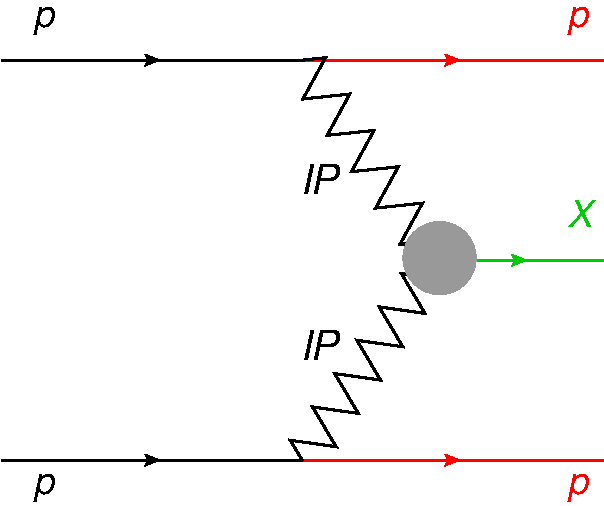
\includegraphics[width=0.92\linewidth]{graphics/introduction/DPE.pdf}\vspace{6pt}%
  \caption{Diagram of D\Pom E process.\\}%
  \label{fig:DPE}\vspace*{-9pt}%
\end{wrapfigure}
%---------------------------

Reaction from Eq.~\eqref{eq:cep} can exhibit purely electromagnetic ($\gamma$-$\gamma$ interaction), mixed ($\gamma$-$\mathcal{O}$ interaction) or purely strong nature ($\mathcal{O}$-$\mathcal{O}$ interaction). The last type is dominant at RHIC energies. It is characterized by the lack of hard scale (if protons are scattered at small angles), therefore perturbative QCD cannot be applied and Regge theory~\cite{IntroductionToRegge} is used instead. An object $\mathcal{O}$ does not have unequivocal QCD representation - in Regge formalism it is the so-called ``trajectory`` (\Reg eggeon, \Reg). \Reg eggeon with quantum numbers of vacuum is called ''\Pomeron`` (\Pom) and \Pom-\Pom\ reaction (Fig.~\ref{fig:DPE}) is called ''Double \Pomeron\  Exchange``. %

%---------------------------
\begin{figure}[b!]
\centering
\parbox{0.475\textwidth}{\vspace{-12pt}%
  \centering%
  \hspace*{-18pt}\includegraphics[width=1.3\linewidth]{graphics/introduction/eta_phi.pdf}\vspace*{-15pt}%
  \caption{CEP represented in $\eta$-$\phi$ space.\\}%
  \label{fig:eta_phi}%
}
\quad\quad
\parbox{0.475\textwidth}{%\vspace{-16pt}%
  \centering%
  \includegraphics[width=0.82\linewidth]{graphics/introduction/CEPatSTAR.pdf}%\vspace{6pt}%
  \caption{Central Production event at STAR.\\}\label{fig:CEPatSTAR}%
%   \hspace*{5pt}
}%\vspace*{-25pt}
\end{figure}
%---------------------------

Processes involing \Pomeron\  exchange are referred as diffraction due to cross-section in scattering angle resembling similar shape to instesity pattern of diffracted light. For low values of Mandelstam $t$ (small scattering angles) cross-section takes exponential form\vspace{-2pt}
\begin{equation}
 \frac{d\sigma}{d|t|} \propto e^{-B|t|},
\end{equation}%
where the slope parameter $B$ reflects the size of target at which \Pomeron s scatter.

Diffractive events have specific property of the ''rapidity gap`` which is an angular region free of hadrons. In \DPE\ two such gaps are present, marked in Fig.~\ref{fig:eta_phi} as $\Delta\eta_{1}$ and $\Delta\eta_{2}$. Figure~\ref{fig:CEPatSTAR} shows the topology of the \DPE\ event on top of the STAR detector, with centrally produced particles marked with green arrows and two forward protons escaping the interaction point inside the beampipe drawn with red arrows.%

\DPE\ is a spin-parity filter - the fact that scattered particles have all quantum numbers unchanged after the interaction, production of central states satisfying Eq.~\eqref{eq:DPE_IGJPC} is enhanced
\begin{equation}\label{eq:DPE_IGJPC}
 I^{G}J^{PC}=0^{+}\textrm{even}^{++}.
\end{equation}%

The lowest order QCD picture of the \Pomeron\ is a pair of oppositely colored gluons (colour singlet). This fact makes the \DPE\ recognized as the gluon-rich environment process in which bound states of gluons (''glueballs``) or hybrid mesons could be preferably produced.

For detailed introduction to the topic of diffraction see Refs.~\cite{pomeronAndQCD,barone}.%\vspace*{-20pt}

% * ** *** **** ***** ****** ******* S E C T I O N ******* ****** ***** **** *** ** *
\section{Physics motivation for the measurement}
STAR collected in 2015 large dataset dedicated for measurement of the Central Diffraction (\DPE\ in particular). Since that year the experiment was enriched with Roman Pot Phase II* subsystem and thus gained possibility of detection of forward protons. It enabled studies of properties of the central state with respect to observables related to exchanged \Pomeron s. No such measurement was performed before at that high c.m.s. energy ($\sqrt{s}=200$~GeV, contamination from \Reggeon\ exchanges is small) which makes it particularly attractive. A brief list of physics issues that can be covered with the study described in this note is briefly introduced below.%
%
\subsection{\DPE\ differential cross-sections, mass spectrum}

As stated in Sec.~\ref{sec:DPE} \DPE\ is a soft process whose theoretical description is done mainly using phenomenological tools, thus measurement of differential cross-sections is needed to verify various production models.

The main focus is put on the simplest state (and most numerously) produced in \DPE, namely a pair of oppositely charged pions, $\pi^{+}\pi^{-}$. It can be formed either in a non-resonant or resonant mechanism. In the first case the $\pi^{+}\pi^{-}$ continuum is formed by the exchange of the off-shell pion between \Pomeron s. Currently there are two models of this reaction on the market~\cite{LSmodel,LSmodel2},~\cite{DurhamModel}. In the second case the \Pomeron s directly couple into resonance (e.g. $f_{2}(1270)$), which then decays to $\pi^{+}\pi^{-}$. Attempts to calculate cross-section for this production mechanism are presented in Ref.~\cite{LSmodel2} and \cite{Schicker}.

Understanding of the mass spectrum in $\pi^{+}\pi^{-}$ channel is important to learn about relative contribution from continuum and resonant production, as well as relative production of resonances. Recognition of resonant states may indicate candidates for low-mass glueballs of $J^{PC}=0^{++}$, however presence of underlaying scalar $q\bar{q}$ states makes this task challenging.

Other channels, like $K^{+}K^{-}$, are also of great interest. Comparison of the cross-sections for production of $\pi^{+}\pi^{-}$ and $K^{+}K^{-}$ gives information about strength of the \Pomeron\ coupling to different quark flavors. Also, structures in $d\sigma/dm$ can be easier attributed to resonances by measuring more than one channel and known branching ratios thereof.

Detection of intact protons scattered at very small angle with respect to the beamline enables determination of the reaction plane which makes the Partial Wave Analysis (PWA) possible. It also allows to look at the the cross-sections more differentially, especially with respect to properties of exchanged \Pomeron s, like carried squared four-momentum $t$, azimuthal separation of \Pomeron s in the transverse plane $\Delta\varphi$ or relative momentum of \Pomeron s $\Delta p_{T}$. The last quantity was proposed to distinguish pure $q\bar{q}$ states from these with gluonic content~\cite{DPtFilter}.

\subsection{Absorption effects}

One can imagine in diagram in Fig.~\ref{fig:DPE} additional soft lines e.g. between protons in the initial state or one of \Pomeron s and final state proton. These so-called rescattering effects (or absorption effects) lead to production of hadrons other than these belonging to central state $X$ hence the diffractive signature of an event in form of rapidity gap is no longer present. Measurement of the probability that the state $X$ will remain exclusive and forward protons will remain intact, in other words the rapidity gap survival probability $S^{2}$, would be valuable ingredient for development of absorption models.

\subsection{Size of interaction region}

From the measurement of protons in Roman Pots one is able to reconstruct squared four-momenta transferred in proton-\Pomeron\ vertices and determine the differential cross-section $d\sigma/d|t|$. Fit of exponent allows to extract the slope parameter $B$, which may depend on the \Pomeron-\Pomeron\ c.m.s. energy, or in other words on the mass of diffractive system $X$. Knowledge on the slope parameter gives insight to the form factor of the object at which \Pomeron\ scatters.


%% =====  DATASET ====
%%===========================================================%%
%%                                                           %%
%%                          DATASET                          %%
%%                                                           %%
%%===========================================================%%


\chapter{Data set}\label{chap:dataset}

\section{Trigger}\label{seq:trigger}

The main trigger designed for studies of Central Diffraction in run 15 was RP\_CPT2. It was formed of the following conditions combined by logical AND (\&\&):
\begin{enumerate}
 \item \textbf{(ET \&\& !IT) $||$ (!ET \&\& IT)} = signal in at least one RP on each side of the STAR central detector - to ensure presence of two forward-scattered protons; a veto was imposed on simultaneous signal in RPs above and below the beamline, which might have originated either from proton dissociation, or pile-up event, or beam halo proton etc.,
 \item \textbf{!BBCE \&\& !BBCW \&\& !ZDCE \&\& !ZDCW} = veto on any signal in small BBC tiles or ZDCs on any side of STAR central detector - such requirement is in accordance with the double-gap topology of CEP events, it mostly filtered out CEP events with parallel pile-up event(s),
 \item \textbf{TOF$\geq$2} = at least 2 hits in TOF - aim of this condition was to ensure activity in the mid-rapidity; since the lowest multiplicity allowed in CEP is 2, that was the lower threshold of L0 TOF multiplicity.
\end{enumerate}%
This trigger was running with an average prescale of 5 and average DAQ rate of 250~Hz, which allowed to collect in total about 560~M events corresponding to 16.5~pb$^{-1}$ of integrated luminosity.  More information about number of events per run, rates etc. can be found under link provided in Ref.~\cite{onlineRpTriggersMonitoring}, which contains selected data from STAR run log~\cite{RunLog}. Luminosity data used in this analysis comes from Ref.~\cite{Luminosity}.

All RP triggers which were intended for usage in diffractive physics analyses or efficiency studies are listed in Tab.~\ref{tab:triggers}. Components used in definitions of these triggers are outlined in Fig.~\ref{fig:triggerBits}. Detailed explanation of all trigger bits can be found in Refs.~\cite{RpTriggers,RpTriggers2}. Explanation of naming convention in Roman Pot system can be found in Ref.~\cite{Labeling}.

\begin{figure}[h]
 \centering%
 \includegraphics[width=0.71\linewidth]{graphics/dataset/bits.png}%
 \caption{Sketch of the trigger components used in definitions of diffractive triggers in run 15.}\label{fig:triggerBits}%
 \end{figure}


\begin{table}[hb!]\centering
 \begin{tabular}{l|c|c|c}%\hline
 \textbf{\specialcell{Trigger\\name}} &  \textbf{Definition} &  \textbf{Events [M]} &  \textbf{Comment} \\ \hline
 RP\_CP & {EOR \&\& WOR} & 73.3 & \specialcell{Loose trigger (mostly elastic events) designed\\for monitoring/trigger efficiency study}\\ \hline
 RP\_CPT & {\specialcell{\specialcell{EOR \&\& WOR\\ \&\& !BBCE \&\& !BBCW} \\ \specialcell{\&\& !ZDCE \&\& !ZDCW} \\ \&\& TOF$\geq$1}} & 38.9 & \specialcell{Intended to be main CEP trigger (later\\switched to RP\_CPT2 due to large prescale)}\\ \hline
 RP\_CPT2 & {\specialcell{\specialcell{(ET \&\& !IT) $||$ (!ET \&\& IT) \\ \&\& !BBCE \&\& !BBCW} \\ \specialcell{\&\& !ZDCE \&\& !ZDCW} \\ \&\& TOF$\geq$2}} & 556.5 & \specialcell{Main CEP trigger\\Note: On Apr 14 added upper TOF limit (10)} \\ \hline
 RP\_CPX & {\specialcell{\specialcell{IT\\ \&\& !BBCE \&\& !BBCW} \\ \specialcell{\&\& !ZDCE \&\& !ZDCW} \\ \&\& TOF$\geq$2}} & 40.1 & \specialcell{The same as RP\_CPT2\\but only IT configuration}\\ \hline
 RP\_CPEI & {\specialcell{\specialcell{ET \&\& IT\\ \&\& !BBCE \&\& !BBCW} \\ \specialcell{\&\& !ZDCE \&\& !ZDCW} \\ \&\& TOF$\geq$2}} & 15.6 & \specialcell{Control trigger for CPT2 to estimate\\ effect of !(ET \&\& IT) veto } %\\ \hline
\end{tabular}\caption{Central Diffraction physics triggers and control triggers involving Roman Pot detectors in run 15.}\label{tab:triggers}
\end{table}


\section{Reconstruction software}\label{sec:recoSoftware}

Raw data was processed with STAR libraries in versions SL17f. All four trigger datasets were processed: production\_pp200trans\_2015, production\_pp200long2\_2015, production\_pp200long3\_2015 and production\_pp200long\_2015 (see~\cite{ProductionList}).

The following BFC options were used in the reconstruction:\vspace{-5pt}
\begin{verbatim}
DbV20160418,pp2015c,btof,mtd,mtdCalib,pp2pp,-beamline,beamline3D,useBTOFmatchOnly,VFStoreX,
fmsDat,fmsPoint,fpsDat,BEmcChkStat,-evout,CorrX,OSpaceZ2,OGridLeak3D,-hitfilt
\end{verbatim}
Main attention should be put on option \textbf{useBTOFmatchOnly} which forced vertexing algorithm to form vertices only from the global TPC tracks which are matched with hits in the TOF system. This solution was found to yield significantly larger signal reconstruction efficiency (vertexing efficiency) and better resolutions. The study which lead to above conclusions, presented in Ref.~\cite{RevertexingProposal}, was performed on the same dataset processed with older libraries SL15k (without useBTOFmatchOnly option).



\section{Data format}\label{sec:dataFormat}

The analyzed data was stored in ROOT files in the picoDST format which was in large part a skimmed MuDST (standard STAR format). The picoDST format was introduced in Ref.~\cite{PicoDstDescription}. PicoDST description files (C++ headers etc.) can be found in the analysis code repository~\cite{AnalysisCodeRepo}.
% 
% \section{Bad runs}\label{sec:badRuns}
% 
% Analysis of CEP was performed on the data from runs with completion status ``Successful'' in the STAR run log. However, based on additional requirements explained below, some runs were omitted from analysis.
% 
% \subsection{RP distance from the beamline}
% 
% 16065025
% 16065026
% 16065027
% 16065028
% 16072057
% 16072058
% 16077055
% 16083006
% 16083007
% 16106031
% 
% %---------------------------
% \begin{figure}[hb]
% \centering
% \parbox{0.4\textwidth}{
%   \centering
%   \begin{subfigure}[b]{\linewidth}{
%                 \subcaptionbox{\label{fig:positionHistograms}}{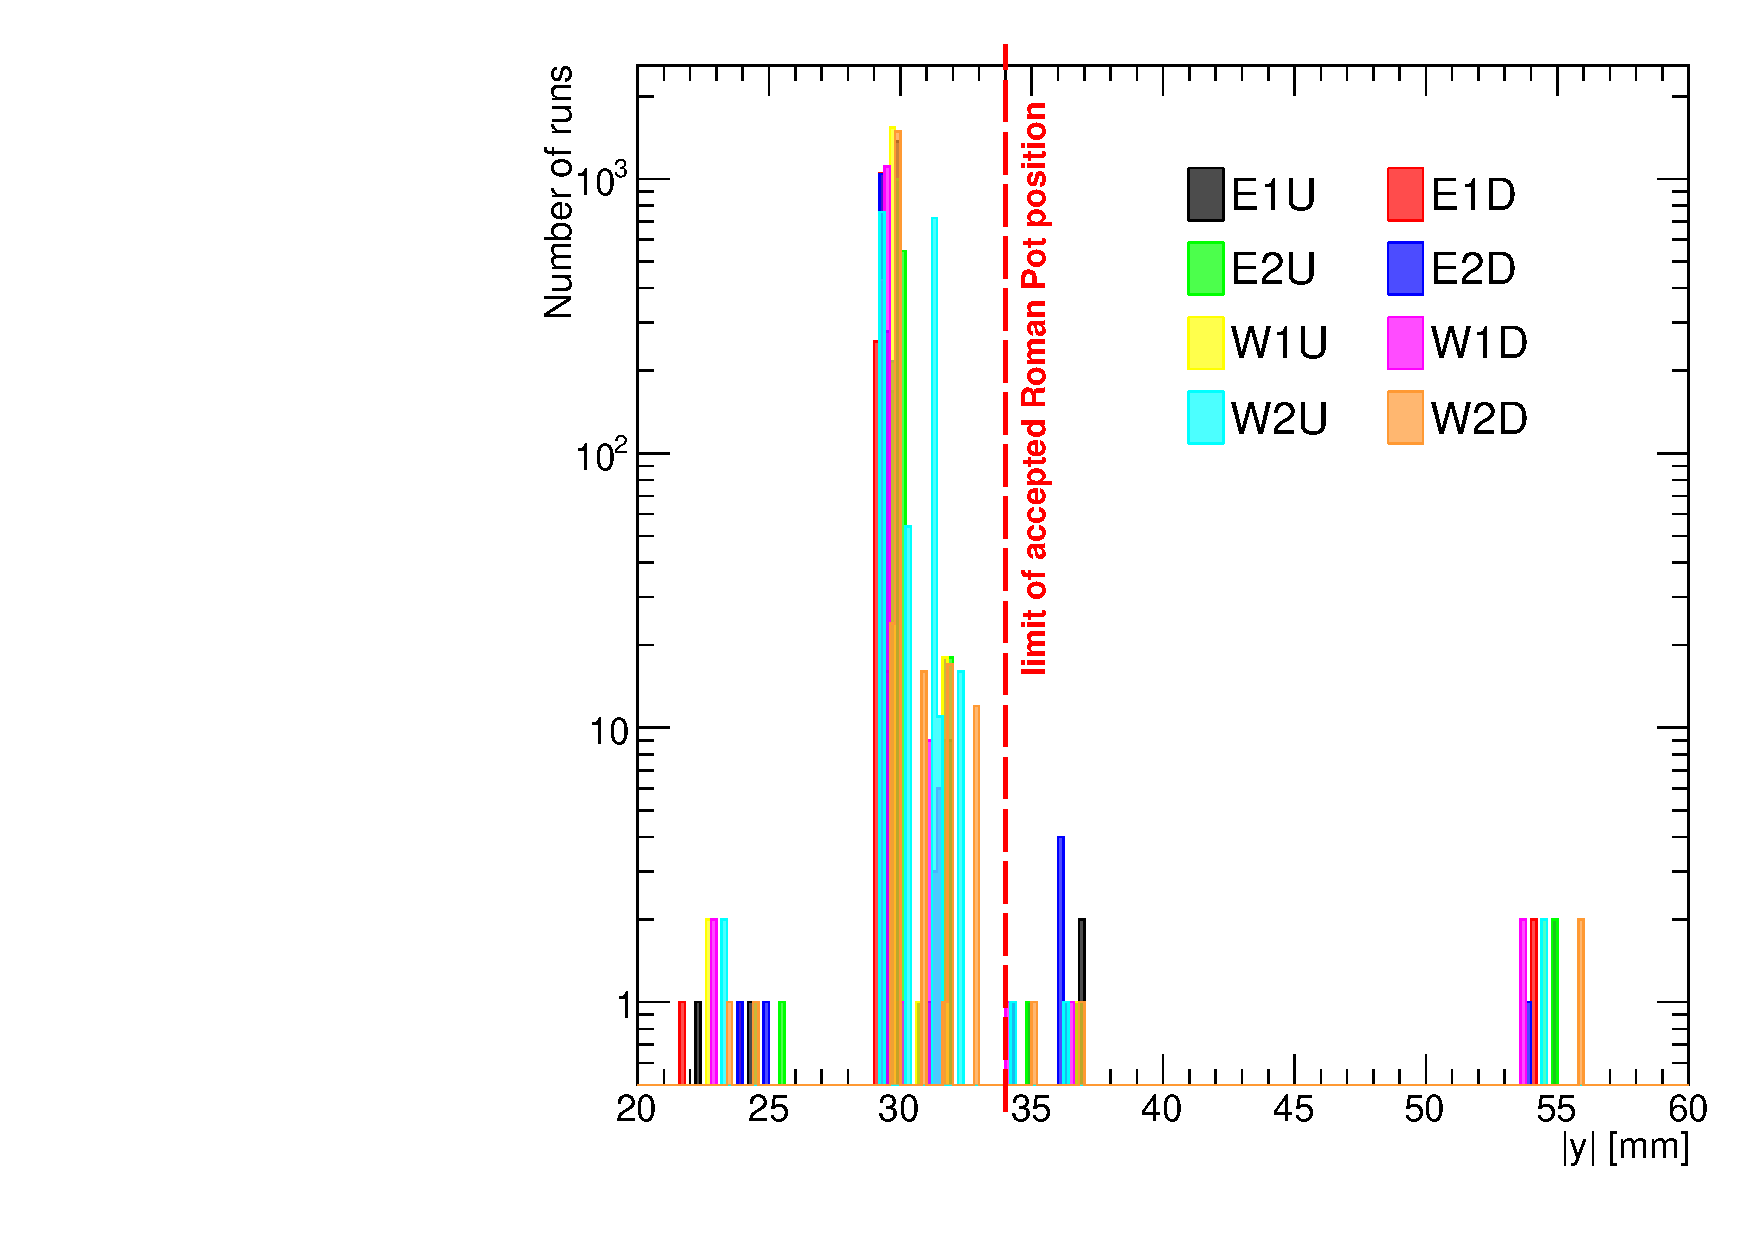
\includegraphics[width=\linewidth]{graphics/dataset/positionHistograms.pdf}}}
%   \end{subfigure}
% }
% \quad
% \parbox{0.545\textwidth}{
%   \centering
%   \begin{subfigure}[b]{\linewidth}{
%                 \subcaptionbox{\label{fig:positionVsRunGraph}}{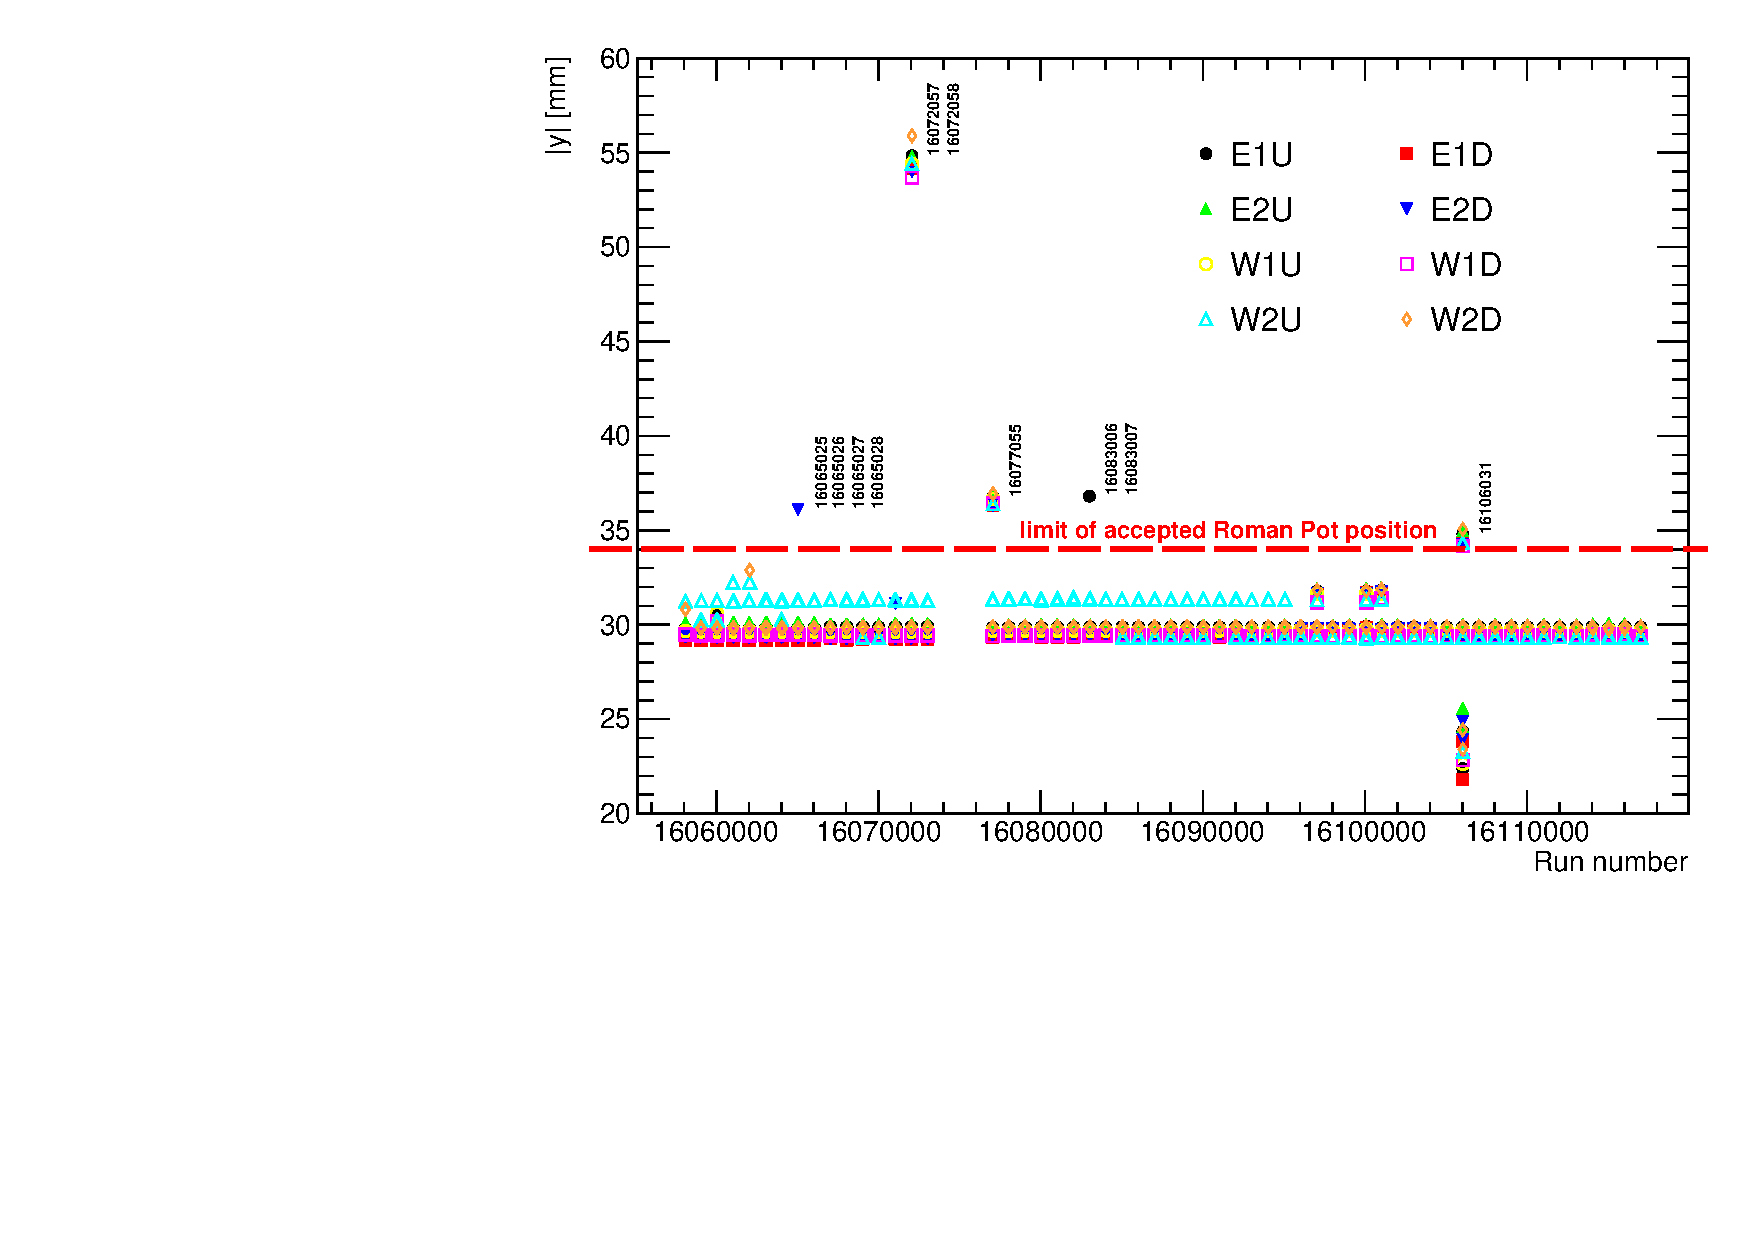
\includegraphics[width=\linewidth]{graphics/dataset/positionVsRunGraph.pdf}}}
%   \end{subfigure}
% }%
% \caption[Beam-detector distance of the Roman Pots in run 15.]{Histogram of beam-detector distance $|y|$ (\ref{fig:positionHistograms}) and graph showing run-dependence of $|y|$ (\ref{fig:positionVsRunGraph}) for all Roman Pots.}%\label{fig:xy_recoEff}
% \end{figure}
% %---------------------------


%% =====  EVENT SELECTION ====
%%===========================================================%%
%%                                                           %%
%%                     EVENT SELECTION                       %%
%%                                                           %%
%%===========================================================%%


\newcommand{\itemm}{\item\hspace*{-5pt}.\hspace*{-1pt}~}

\chapter{Event selection}\label{chap:eventSelection}

Complete list of analysis cuts used for signal extraction is presented in Sec.~\ref{sec:listOfCuts}. Detailed description of each cut can be found in Sec.~\ref{sec:descriptionOfCuts}. [For PDF readers: you can directly move to description of given cut by clicking on corresponding bold cut number \textbf{CX} at the start of line in the list of cuts.]

\section[List of cuts]{List of cuts\footnote{Some cuts (e.g.~\ref{enum:CutTpcTrks}) are decomposed to constituent sub-cuts. Cut is formed by the logical AND of all its sub-cuts. Events must pass all cuts to be identified as a signal.}}\label{sec:listOfCuts}
\begin{enumerate}[label=\textbf{\hyperref[sec:C\arabic*]{C\arabic*}},ref=C\arabic*]
 \itemm Exactly 1 primary vertex with TPC track(s) matched with hits in TOF.\label{enum:CutPrimVx}
 \itemm TPC vertex from~\ref{enum:CutPrimVx} is placed within $|z_{\text{vx}}|<80$~cm.\label{enum:CutZVx}
 \itemm Exactly 2 opposite-sign primary TPC tracks~(\ref{enum:TpcOppoSign}) of good quality~(\ref{enum:TpcQualityCuts}) matched with hits in TOF~(\ref{enum:TpcTofMatched}) and reconstructed within kinematic region of high TPC acceptance~(\ref{enum:TpcKinematicCuts}), with associated global tracks characterized by small distance of closest approach (DCA) to the primary vertex~(\ref{enum:TpcDcaCuts}) and high proximity to each other at the beamline~(\ref{enum:TpcDeltaZ0Cut}).\label{enum:CutTpcTrks}
    \begin{enumerate}[label=\textbf{\theenumi.\arabic*},ref=\theenumi.\arabic*]
      \itemm Exactly 2 TOF-matched (match flag $>0$) primary tracks and no additional primary tracks matched with BEMC clusters,\label{enum:TpcTofMatched}
      \itemm Tracks are of opposite signs,\label{enum:TpcOppoSign}
      \itemm Both tracks are contained within the kinematic range:\label{enum:TpcKinematicCuts}\hspace*{13pt}
      $|\eta|<0.7$,~~~~$p_{T}>0.2~\text{GeV}$,
      \itemm Associated global tracks satisfy quality criteria:\label{enum:TpcQualityCuts}\hspace*{44pt}
      $N_{\text{hits}}^{\text{fit}}\geq25$,~~~$N_{\text{hits}}^{\text{dE/dx}}\geq15$,~~~$|d_{0}|<1.5$~cm,
      \itemm Associated global tracks match well to the prim. vertex:\label{enum:TpcDcaCuts}\hspace*{3.5pt}
      $\text{DCA}(R)<1.5$~cm,~~~~$|\text{DCA}(z)|<1$~cm,
      \itemm Associated global tracks are close at the beamline:\label{enum:TpcDeltaZ0Cut}\hspace*{29pt}
      $|\Delta z_{0}|<2$~cm.
    \end{enumerate}
 \itemm Exactly 1 RP track on each side of STAR central detector~(\ref{enum:RpOneTrkPerSide}) of good quality~(\ref{enum:RpQualityCuts}), with local angles consistent with the IP being the track origin~(\ref{enum:RpLocalAngles}), lying within fiducial region of high geometrical acceptance~(\ref{enum:RpFiducial}).\label{enum:CutRpTrks}
      \begin{enumerate}[label=\textbf{\theenumi.\arabic*},ref=\theenumi.\arabic*]
      \itemm RP tracks contain only track-points with at least 3 (out of 4) planes used in reconstruction,\label{enum:RpQualityCuts}
      \itemm Local angles ($\theta_{x}^{\text{RP}}$, $\theta_{y}^{\text{RP}}$) consistent with expectation for protons originating from the IP\label{enum:RpLocalAngles}%
      \[-2~\text{mrad}<\theta_{x}^{\text{RP}}-x^{\text{RP}}/|z^{\text{RP}}|<4~\text{mrad},~~~~~-2~\text{mrad}<\theta_{y}^{\text{RP}}-y^{\text{RP}}/|z^{\text{RP}}|<2~\text{mrad},\]
      \itemm Exactly 1 track passing cuts \ref{enum:RpQualityCuts}-\ref{enum:RpLocalAngles} per side,\label{enum:RpOneTrkPerSide}
      \itemm Tracks passing cut~\ref{enum:RpOneTrkPerSide} lie within the fiducial $(p_{x},p_{y})$ region defined as\vspace*{-7pt}\label{enum:RpFiducial}:\\
      \[0.2<|p_{y}|<0.4,~~~-0.2<p_{x},~~~(p_{x}+0.3)^{2}+p_{y}^{2}<0.5^{2}~~~(\text{all in GeV}).\]
    \end{enumerate}
 \itemm Vertex $z$-positions measured in TPC and reconstructed from the difference of proton detection time in west and east RPs are consistent with each other within the resolution (at $3.5\sigma_{\Delta z_{\text{vtx}}}$ level):
 \[|\Delta z_{\text{vtx}}| = |z_{\text{vx}}^{\text{TPC}}-z_{\text{vx}}^{\text{RP}}|<36~\text{cm}.\vspace{-17pt}\]\label{enum:CutDeltaZVx}
 \itemm No signal in any tile of BBC-large (east or west) with $\text{ADC}>\text{ADC}_{\text{thr}}$ and $100<\text{TDC}<2400$, where $\text{ADC}_{\text{thr}}$ is specific for each channel (see Tab.~\ref{tab:bbcLargeThresholds}).\label{enum:CutBbcLarge}%
 %
 \itemm Maximally 3 reconstructed TOF clusters $N^{\text{TOF}}_{\text{clstrs}}\leq 3$.\label{enum:CutTofClusters}%
 %
 \itemm Particle/pair identification (PID):\label{enum:CutPid}
 \begin{enumerate}[label=\textbf{\theenumi.\arabic*},ref=\theenumi.\arabic*]
      \itemm Identification of particle pairs based on $dE/dx$ ($\chi^{2}$) and $m^{2}_{\text{TOF}}$ (def. in Sec.~\ref{sec:C8} and App.~\ref{appendix:squaredMass}):\label{enum:CutPidNoPtLimit}\\[3pt]
        \textbf{~~if~~~}\hspace*{4.5pt}$\chi^{2}(\pi\pi)>9$\textbf{~~and~~}$\chi^{2}(KK)>9$\textbf{~~and~~}$\chi^{2}(pp)<9$\textbf{~~and~~}$m^{2}_{\text{TOF}}>0.6~\text{GeV}~~\rightarrow~~p\bar{p}$\\[5pt]%
        %
        \textbf{elif~~}$\chi^{2}(\pi\pi)>9$\textbf{~~and~~}$\chi^{2}(KK)<9$\textbf{~~and~~}$\chi^{2}(pp)>9$\textbf{~~and~~}$m^{2}_{\text{TOF}}>0.15~\text{GeV}~~\rightarrow~~K^{+}K^{-}$\\[5pt]%
        %
        \textbf{elif~} $\chi^{2}(\pi\pi)<12~~\rightarrow~~\pi^{+}\pi^{-}$.%~~~~~~~~~~~~~~~~~~~~~~~~~~~~~~~\textbf{otherwise~~} event rejected.
      \itemm Restricting fiducial cuts on $K^{+}K^{-}$ and $p\bar{p}$ (to reduce misidentifications and assure high PID eff.):\label{enum:CutPidPtLimits}\\[2pt]
      \textbf{~if~} $K^{+}K^{-}$:~~~~~~$p_{T}>0.3~\text{GeV}$,~~~~$min(p_{T}^{+},p_{T}^{-})<0.7~\text{GeV}$\\[2pt]%
      \textbf{~if~} $p\bar{p}$:~~~~~~~~~~~~\hspace*{1.7pt}$p_{T}>0.4~\text{GeV}$,~~~~$min(p_{T}^{+},p_{T}^{-})<1.1~\text{GeV}$%
\end{enumerate}
\itemm Missing (total) momentum of TPC tracks and RP tracks $p_{T}^{\text{miss}}<75~\text{MeV}$.\label{enum:CutMissingPt}%
 %
 
\end{enumerate}
%
%
%
%
%
\section{Description of cuts}\label{sec:descriptionOfCuts}%
%
\subsection{(\ref{enum:CutPrimVx},\ref{enum:CutZVx})~Primary vertex and its \texorpdfstring{$z$}{z}-position}\label{sec:C1}\label{sec:C2}
As it was designed in the trigger logic, we aim to perform CEP analysis in a clean, pile-up-free environment, therefore we cut on primary vertex multiplicity~(Fig.~\ref{fig:NumberOfPrimaryVertices}) to reject events with more than one interaction per bunch crossing. We required exactly one primary vertex containing TPC tracks matched with hits in TOF (matching of the track with hit in TOF is identified with the TOF match flag being different from 0). Later in the text we refer to such events as a single ``TOF vertex`` events.

%---------------------------
\begin{figure}[ht!]%
\centering%
\begin{minipage}{.4725\textwidth}%
  \centering%
  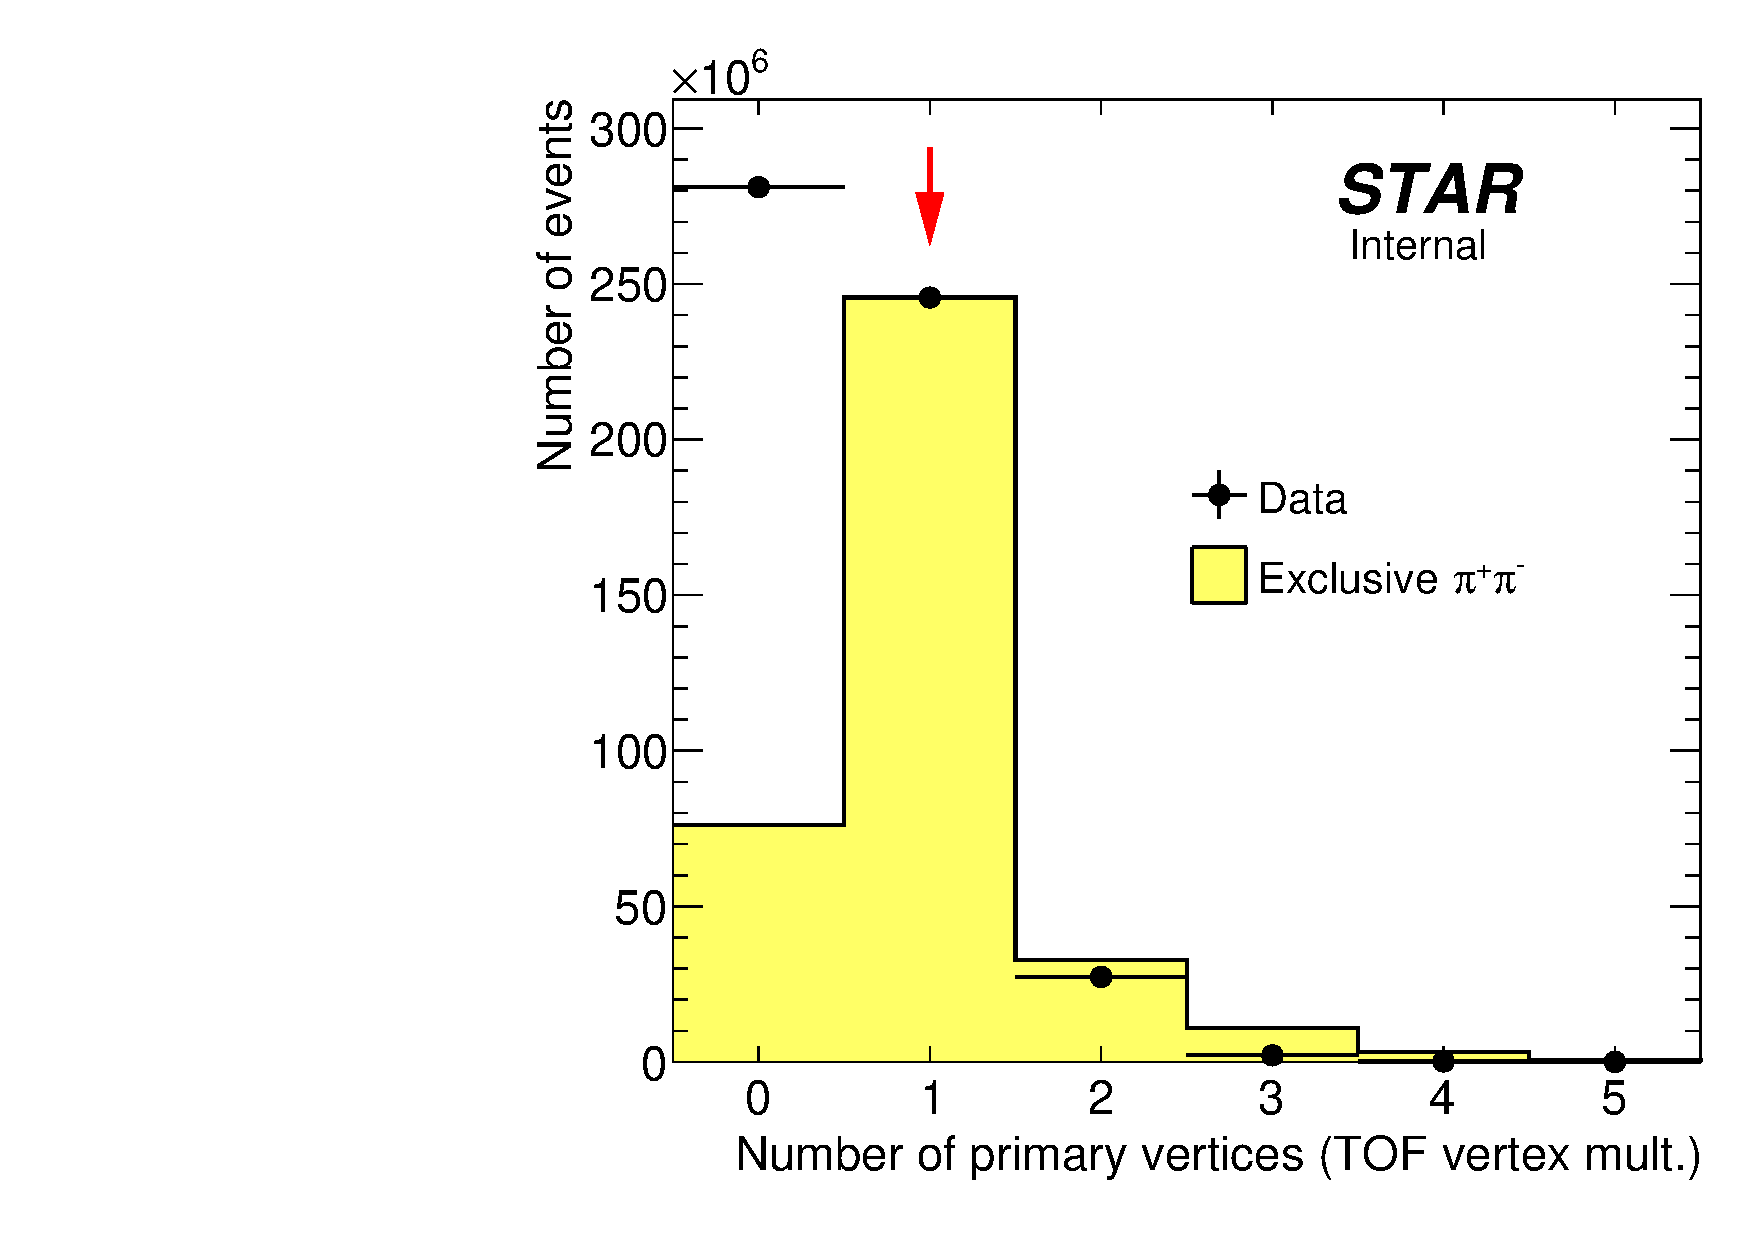
\includegraphics[width=\linewidth]{graphics/eventSelection/NumberOfPrimaryVertices.pdf}%
  \caption{Primary vertex multiplicity. Red arrow marks bin with events with exactly one primary vertex (with track(s) matched with hit in TOF), which are used in physics analysis.}\label{fig:NumberOfPrimaryVertices}
\end{minipage}%
\quad\quad%
\begin{minipage}{.4725\textwidth}%
  \centering
  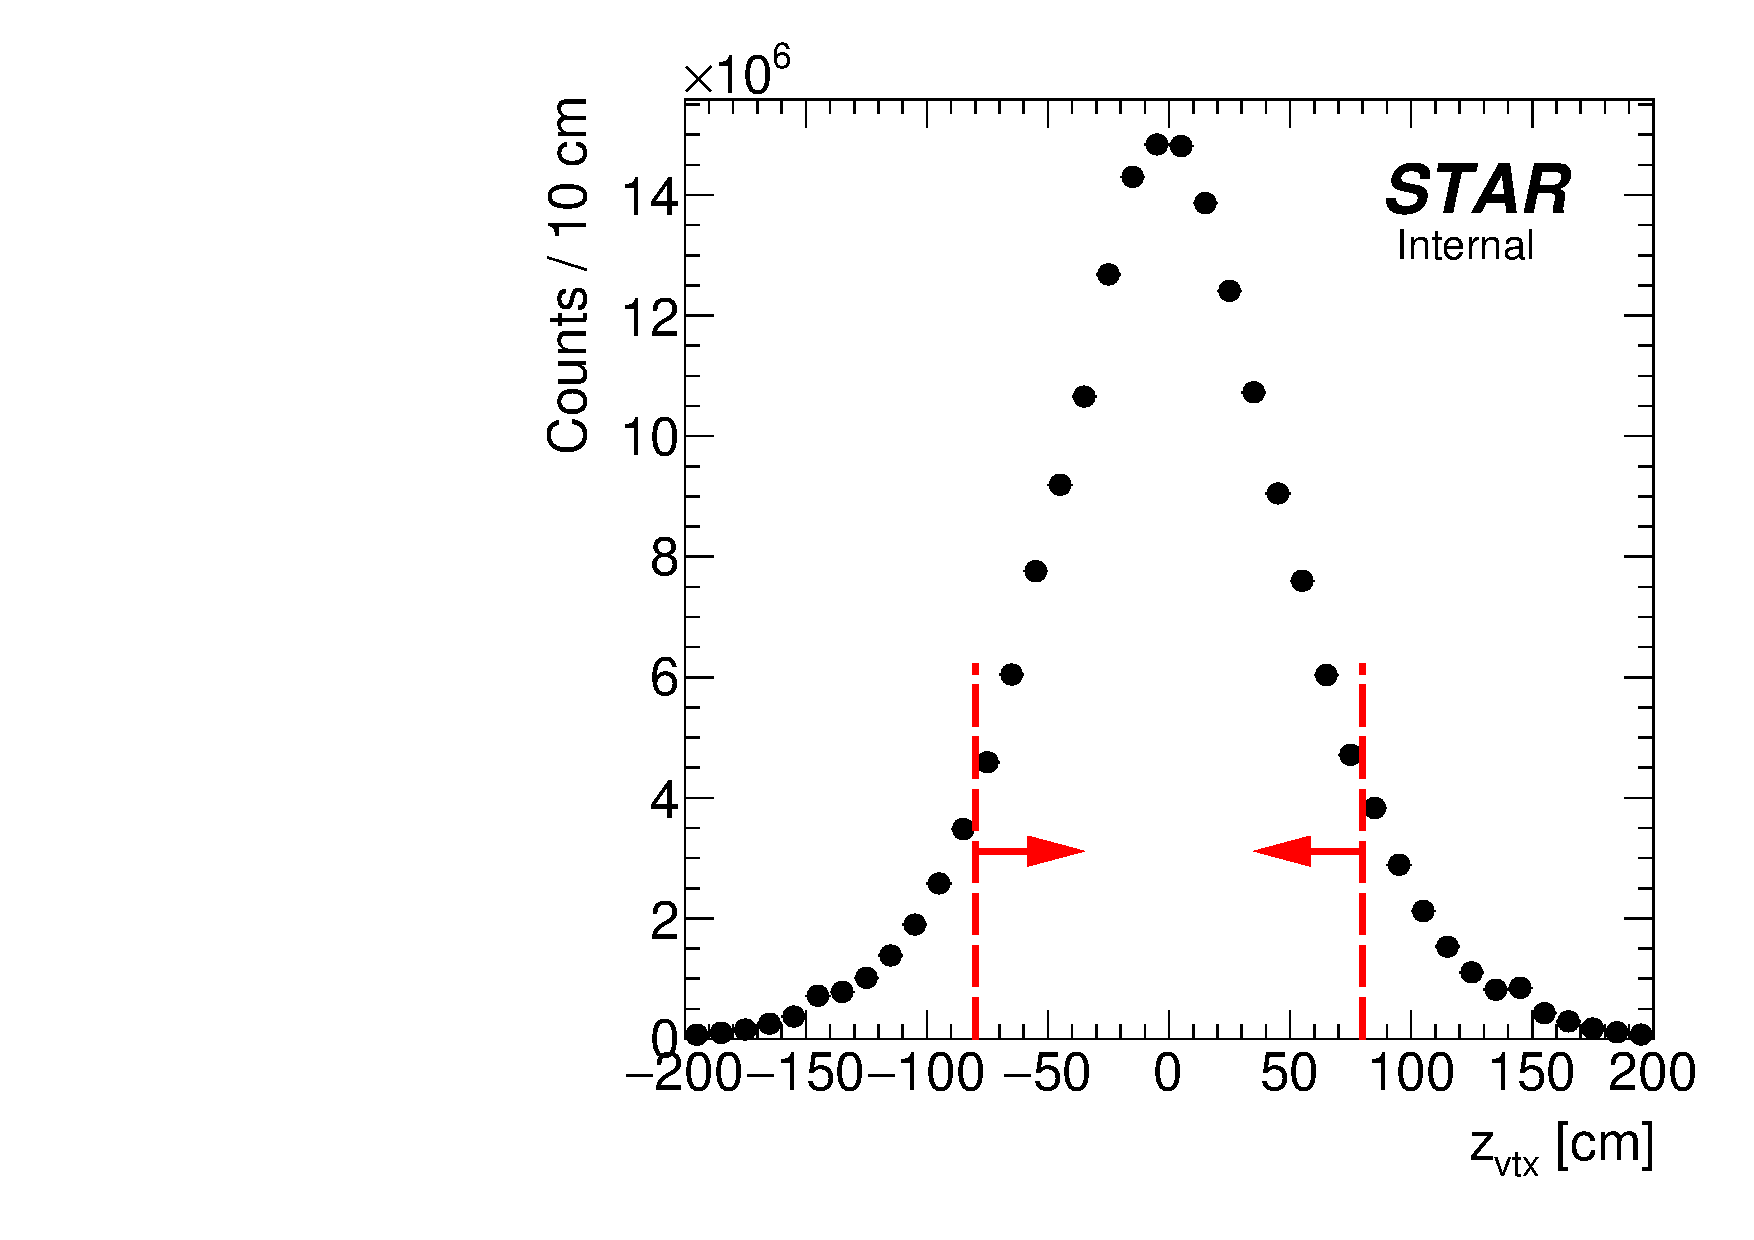
\includegraphics[width=\linewidth]{graphics/eventSelection/zVertex_oneTof.pdf}%
  \caption{\texorpdfstring{$z$}{z}-position of the primary vertex in single TOF vertex events (passing cut~\ref{enum:CutPrimVx}). Red dashed line indicate range of longitudinal vertex position accepted in analysis.}\label{fig:zVertexTpc}
\end{minipage}%
\end{figure}%
%---------------------------


The single TOF vertex was required to be placed within a range $(-80~\text{cm},~80~\text{cm})$ along the $z$-axis~(Fig.~\ref{fig:zVertexTpc}). Events with vertices away from the nominal IP have low acceptance both for the central tracks and the forward protons (comparing to events with vertices close to nominal IP), therefore we reject them as their inclusion to analysis would naturally introduce large systematic uncertainties. See Sec.~3.2.3 in Ref.~\cite{supplementaryNote}.

%---------------------------
\begin{figure}[h]
\centering%
\parbox{0.5325\textwidth}{%
  \centering%
  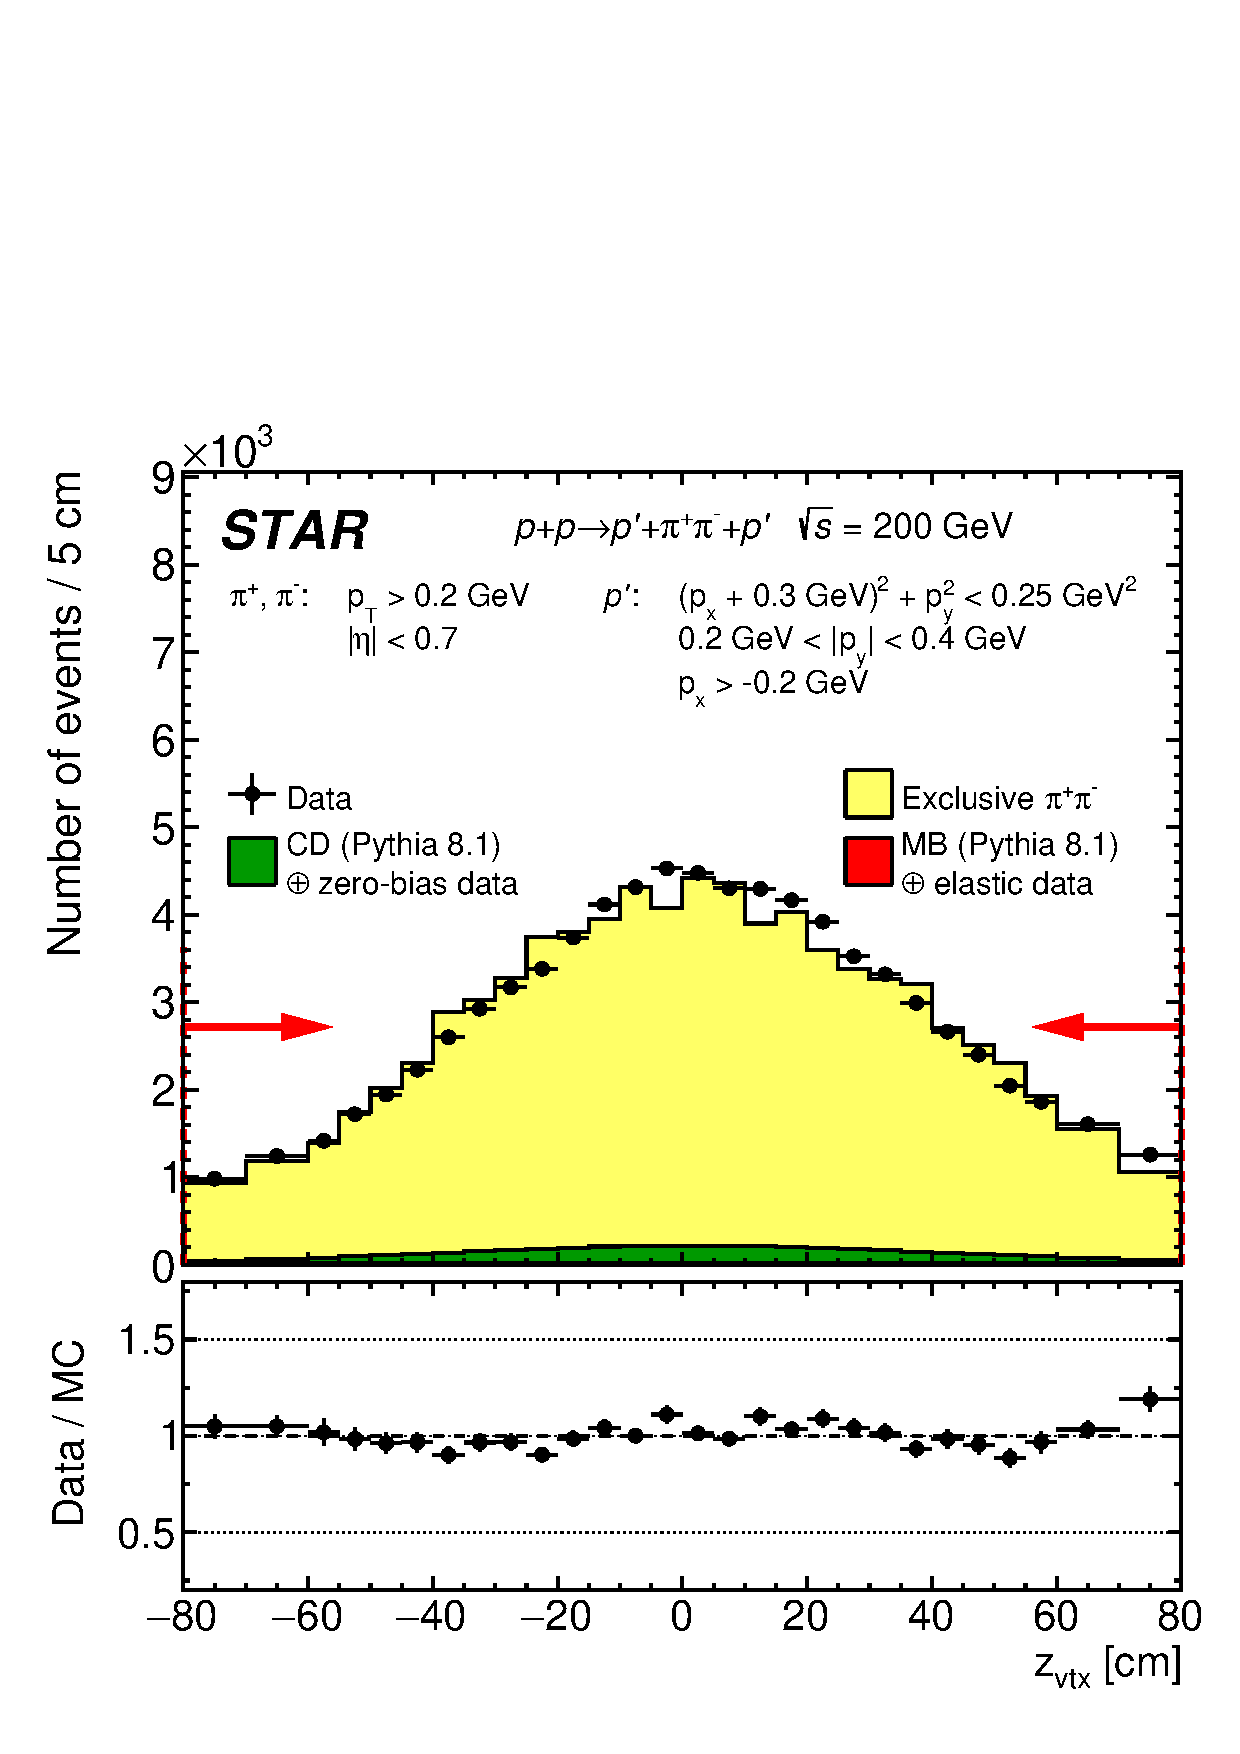
\includegraphics[width=\linewidth]{graphics/backgrounds/dataVsMc/Ratio_Linear_ZVtx.pdf} 
}%
\quad%
\parbox{0.4125\textwidth}{%
    \caption[Comparison of $z_{\text{vtx}}$ distribution between data and embedded MC.]{Comparison of $z_{\text{vtx}}$ distribution between data and embedded MC after full selection. Data are represented by black points, while stacked MC predictions are drawn as histograms of different colors. Histogram from each MC process has been normalized according to prescription in Sec.~\ref{sec:bkgdSignalNorm}. Vertical error bars represent statistical uncertainties, horizontal bars represent bin sizes. Comparison is shown for only $z$-vertex range corresponding to offline selection cut~\ref{enum:CutZVx} due to such limited vertex range used in MC generation for increase of generation efficiency.}\label{fig:Ratio_Linear_ZVtx} %  
}
\end{figure}
%---------------------------


In Fig~\ref{fig:Ratio_Linear_ZVtx} we show comparison of the $z$-position of single TOF primary vertex measured in the TPC, between data and MC generated e.g. to study of detector effects present in analysis. The ratio of distributions which is compatible with unity indicates proper position, width and shape of distribution assumed at MC generation (gaussian with mean at 0 and width of 50~cm).




\subsection{(\ref{enum:CutTpcTrks})~TPC tracks}\label{sec:C3}

The TPC track selection starts from the selection of events with exactly two primary tracks matched with hit in TOF~(Fig.~\ref{fig:NumberOfTofTracksInSingleTofVertex}). Matching with TOF guarantee that analyzed tracks originate from the triggered bunch crossing (ensures that tracks are ''in-time``). It is in accordance with the trigger logic which required at least 2 L0 TOF hits, as well as it enables more accurate particle identification with merged time-of-flight and $dE/dx$ method, comparing to sole usage of $dE/dx$. Primary tracks not matched with hit in TOF, whose average multiplicity in single TOF vertex is $\sim$8, are hardly distinguished between real and fake (off-time) tracks, which is an additional reason for not analyzing events with only one TOF-matched primary TPC track (the other track might be unmatched due to TOF inefficiency).

%---------------------------
\begin{figure}[t!]%
\centering%
\begin{minipage}{.4725\textwidth}%
  \centering%
  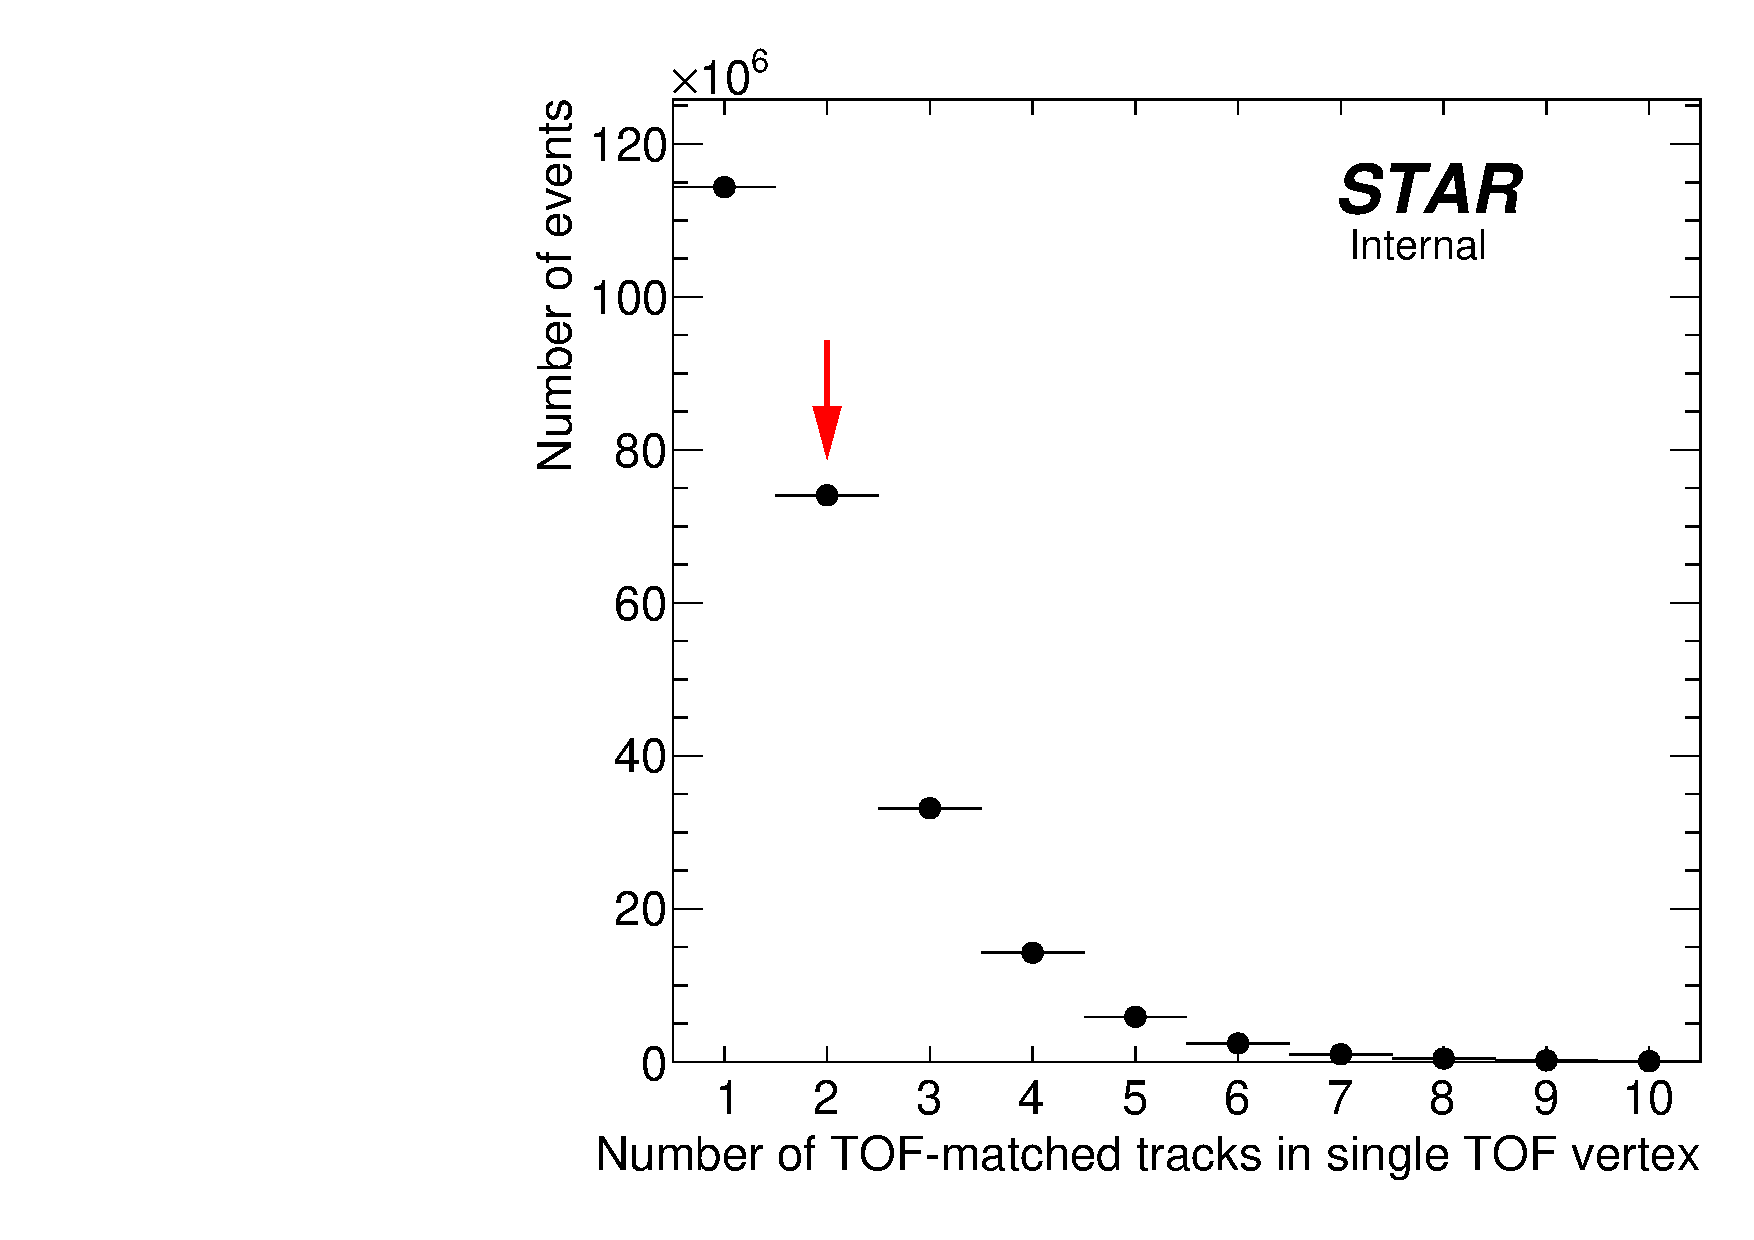
\includegraphics[width=\linewidth]{graphics/eventSelection/TpcTracks/NumberOfTofTracksInSingleTofVertex.pdf}%
  \caption[Multiplicty of primary TPC tracks matched with hit in TOF for single TOF vertex events]{Multiplicty of primary TPC tracks matched with hit in TOF for single TOF vertex events. Red arrow marks bin with events with exactly two primary tracks matched with hit in TOF, which are used in physics analysis.\newline}\label{fig:NumberOfTofTracksInSingleTofVertex}
\end{minipage}%
\quad\quad%
\begin{minipage}{.4725\textwidth}%
  \centering
  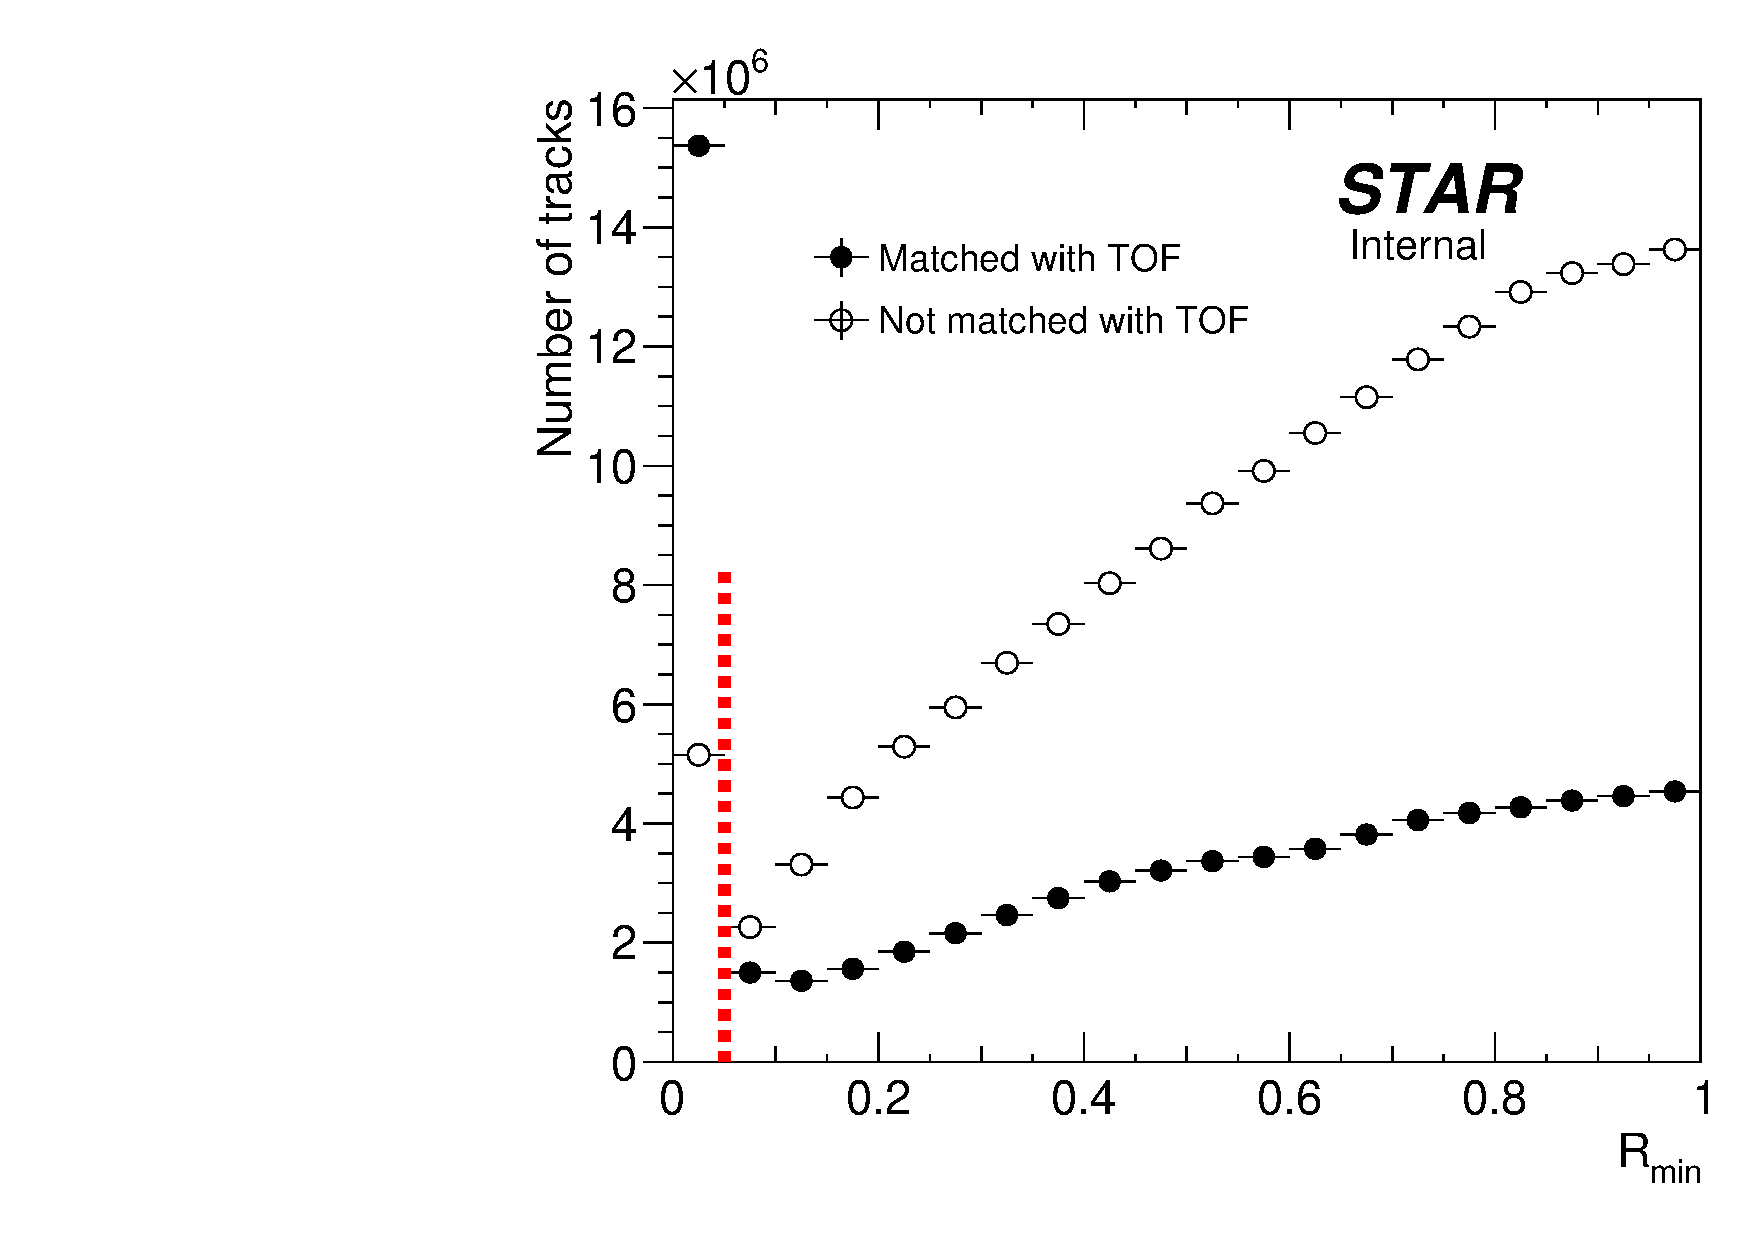
\includegraphics[width=\linewidth]{graphics/eventSelection/TpcTracks/Rmin.pdf}%
  \caption[Distribution of a distance in $\eta-\phi$ space between the BEMC cluster closest to primary TPC track ($R_{\text{min}}$)]{Distribution of a distance in $\eta-\phi$ space between the BEMC cluster closest to primary TPC track matched (filled circle) or not matched (opened circle) with hit in TOF, for single TOF vertex events. Red dashed line indicate matching threshold $R^{\text{match}}_{\text{max}} = 0.05$.}\label{fig:Rmin} %which are expected to reack BEMC
\end{minipage}%
\end{figure}%
%---------------------------

Primary TPC tracks from the single TOF vertex which are matched with TOF are allowed to be also matched with BEMC clusters. Matching with BEMC cluster is claimed if the distance in $\eta-\phi$ space between the BEMC cluster position $(\eta_{\text{clus}},~\phi_{\text{clus}})$ and projected position of the track in BEMC $(\eta_{\text{proj}},~\phi_{\text{proj}})$, defined as
\begin{equation}\label{eq:etaPhiR}
 R=\sqrt{(\eta_{\text{clus}}-\eta_{\text{proj}})^{2} + (\phi_{\text{clus}}-\phi_{\text{proj}})^{2}},
\end{equation}
is less than $R^{\text{match}}_{\text{max}} = 0.05$. Distribution of the distance between the primary TPC track and the closest BEMC cluster is shown in~Fig.~\ref{fig:Rmin}.

However, if there are any primary TPC tracks matched with BEMC cluster and not matched with TOF in the single TOF vertex with two TOF-matched tracks, an event is rejected. Such configuration implies higher-than-2 multiplicity of the real tracks in the vertex, hence an event is unlikely a Central Exclusive Production of two particles.

We apply cuts on the quantities reflecting quality of reconstructed TPC tracks similar to these typically used at STAR. We cut on number of hits used in TPC track reconstruction $N_{\text{hits}}^{\text{fit}} \geq 25$ and number of hits used in specific energy loss reconstruction $N_{\text{hits}}^{\text{dE/dx}} \geq 15$ in order to achieve good momentum and $dE/dx$ resolution. We show distributions of aforementioned quantities together with spectrum of fraction of number of hits potentially generated by the track and finally used in the reconstruction $N_{\text{hits}}^{\text{fit}}/N_{\text{hits}}^{\text{poss}}$ in Fig.~\ref{fig:NHits}. One can see, that embedded MC simulation describes measured data well.

We also require that helices of global tracks associated with selected primary TOF tracks point well to the primary vertex ($\text{DCA}(R)<1.5$~cm and $|\text{DCA}(z)|<1$~cm), as well as the longitudinal separation of helices at the beamline (Fig.~\ref{fig:deltaZ0Sketch}) is small and coincides with cut on $|\text{DCA}(z)|$ ($|\Delta z_{0}|<2$~cm). Distributions of these quantities together with comparison against embedded MC are shown in Fig.~8.5 of Ref.~\cite{supplementaryNote}. In that reference one can also read how appropriate adjustment was derived needed to achieve satisfactory agreement of the $d_{0}$, $\text{DCA}(R)$, $\text{DCA}(z)$ and $|\Delta z_{0}|$ in data and embedded MC.

Figure~\ref{fig:TrackEtaPhi} shows comparison of the track pseudorapidity and azimuthal angle between data and embedded MC. These distributions are quite well described by MC. Large modulation in the $\phi$ distribution (enhancement at $\phi=\pm\pi/2$) is connected with the RP acceptance mostly at $\varphi=\pm\pi/2$ - central particles pair is always back-to-back in azumith with respect to pair of forward scattered protons, therefore pairs produced in ''up`` or ''down`` direction are preferred.

%---------------------------
\begin{figure}[hb]
\centering
\parbox{0.4725\textwidth}{
  \centering
  \begin{subfigure}[b]{\linewidth}
                \subcaptionbox{\label{fig:NHitsFit}}{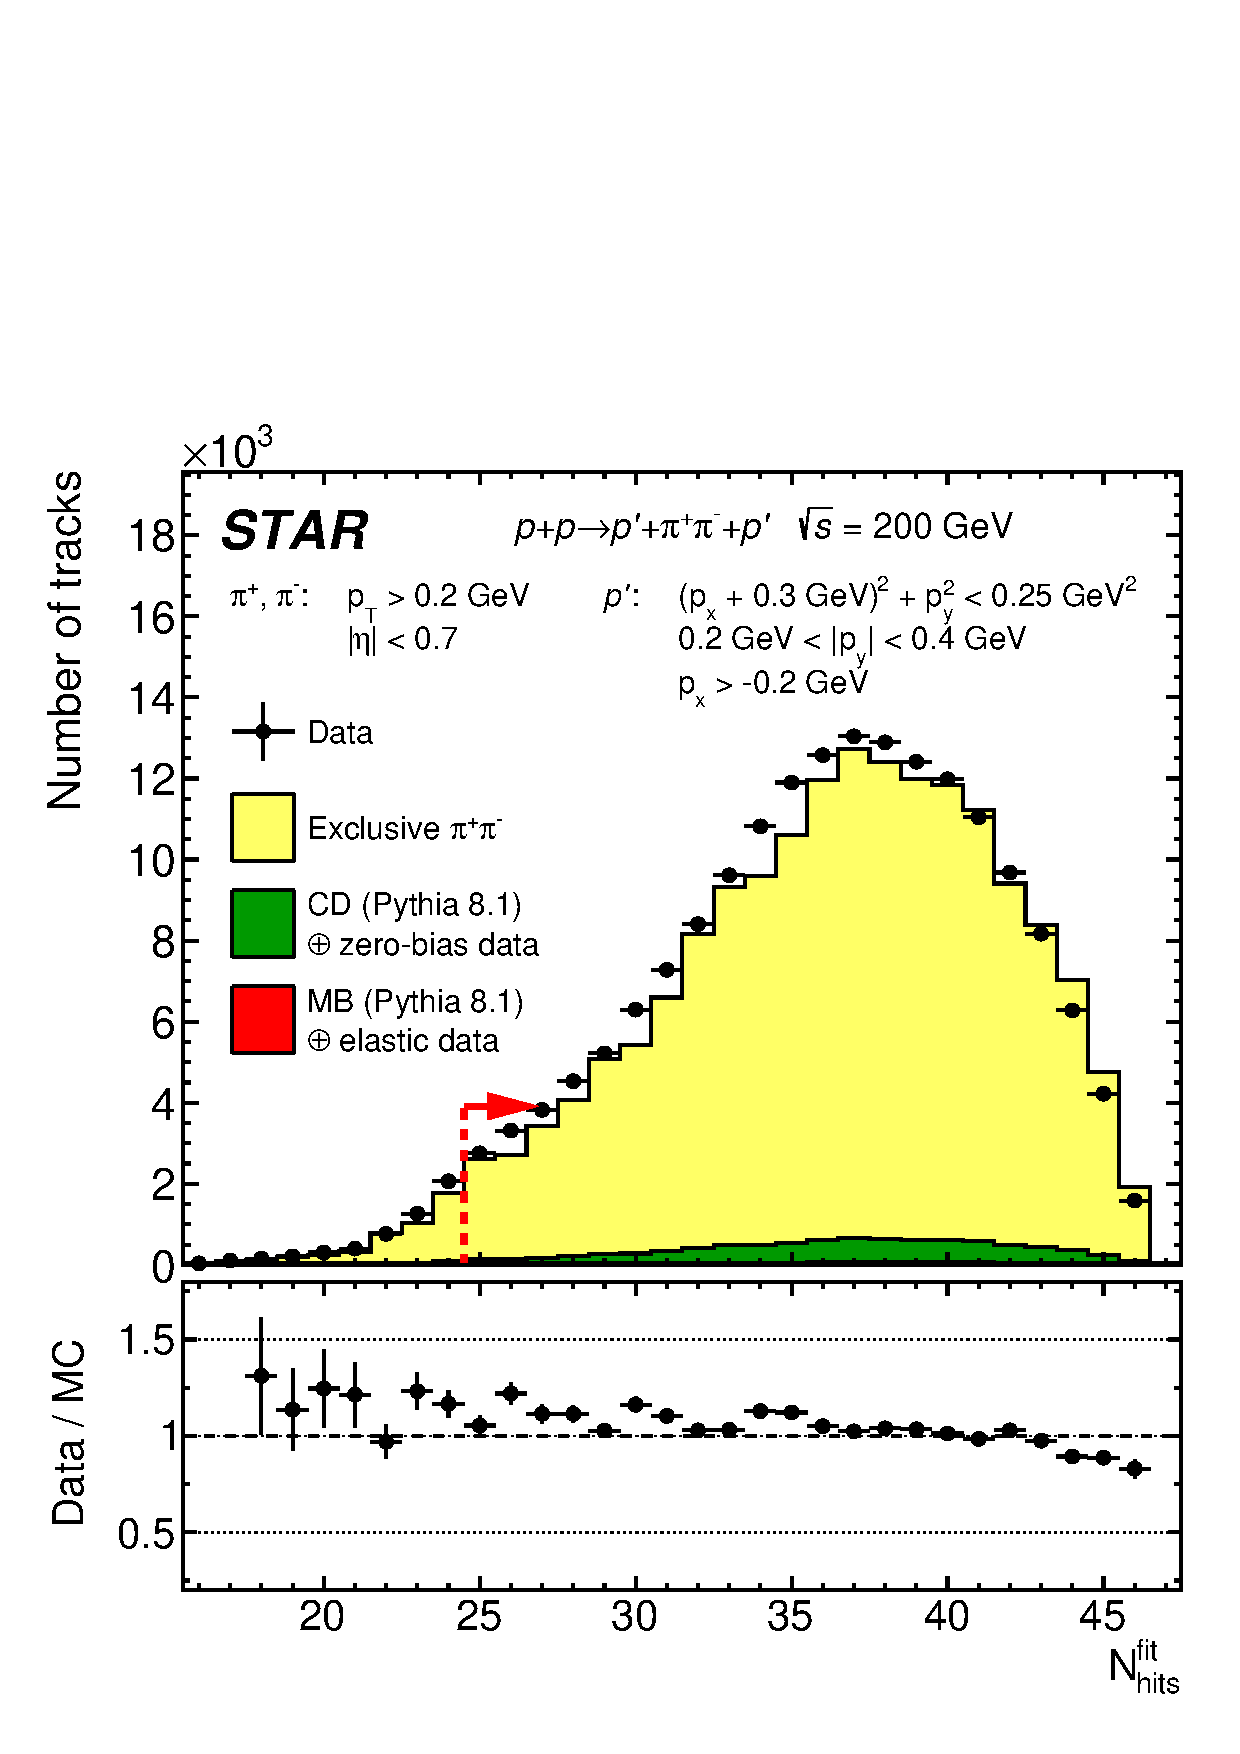
\includegraphics[width=\linewidth]{graphics/eventSelection/TpcTracks/Ratio_Linear_NHitsFit.pdf}}
  \end{subfigure}\\
  \begin{subfigure}[b]{\linewidth}\addtocounter{subfigure}{1}
                \subcaptionbox{\label{fig:NHitsFit_to_NHitsPos}}{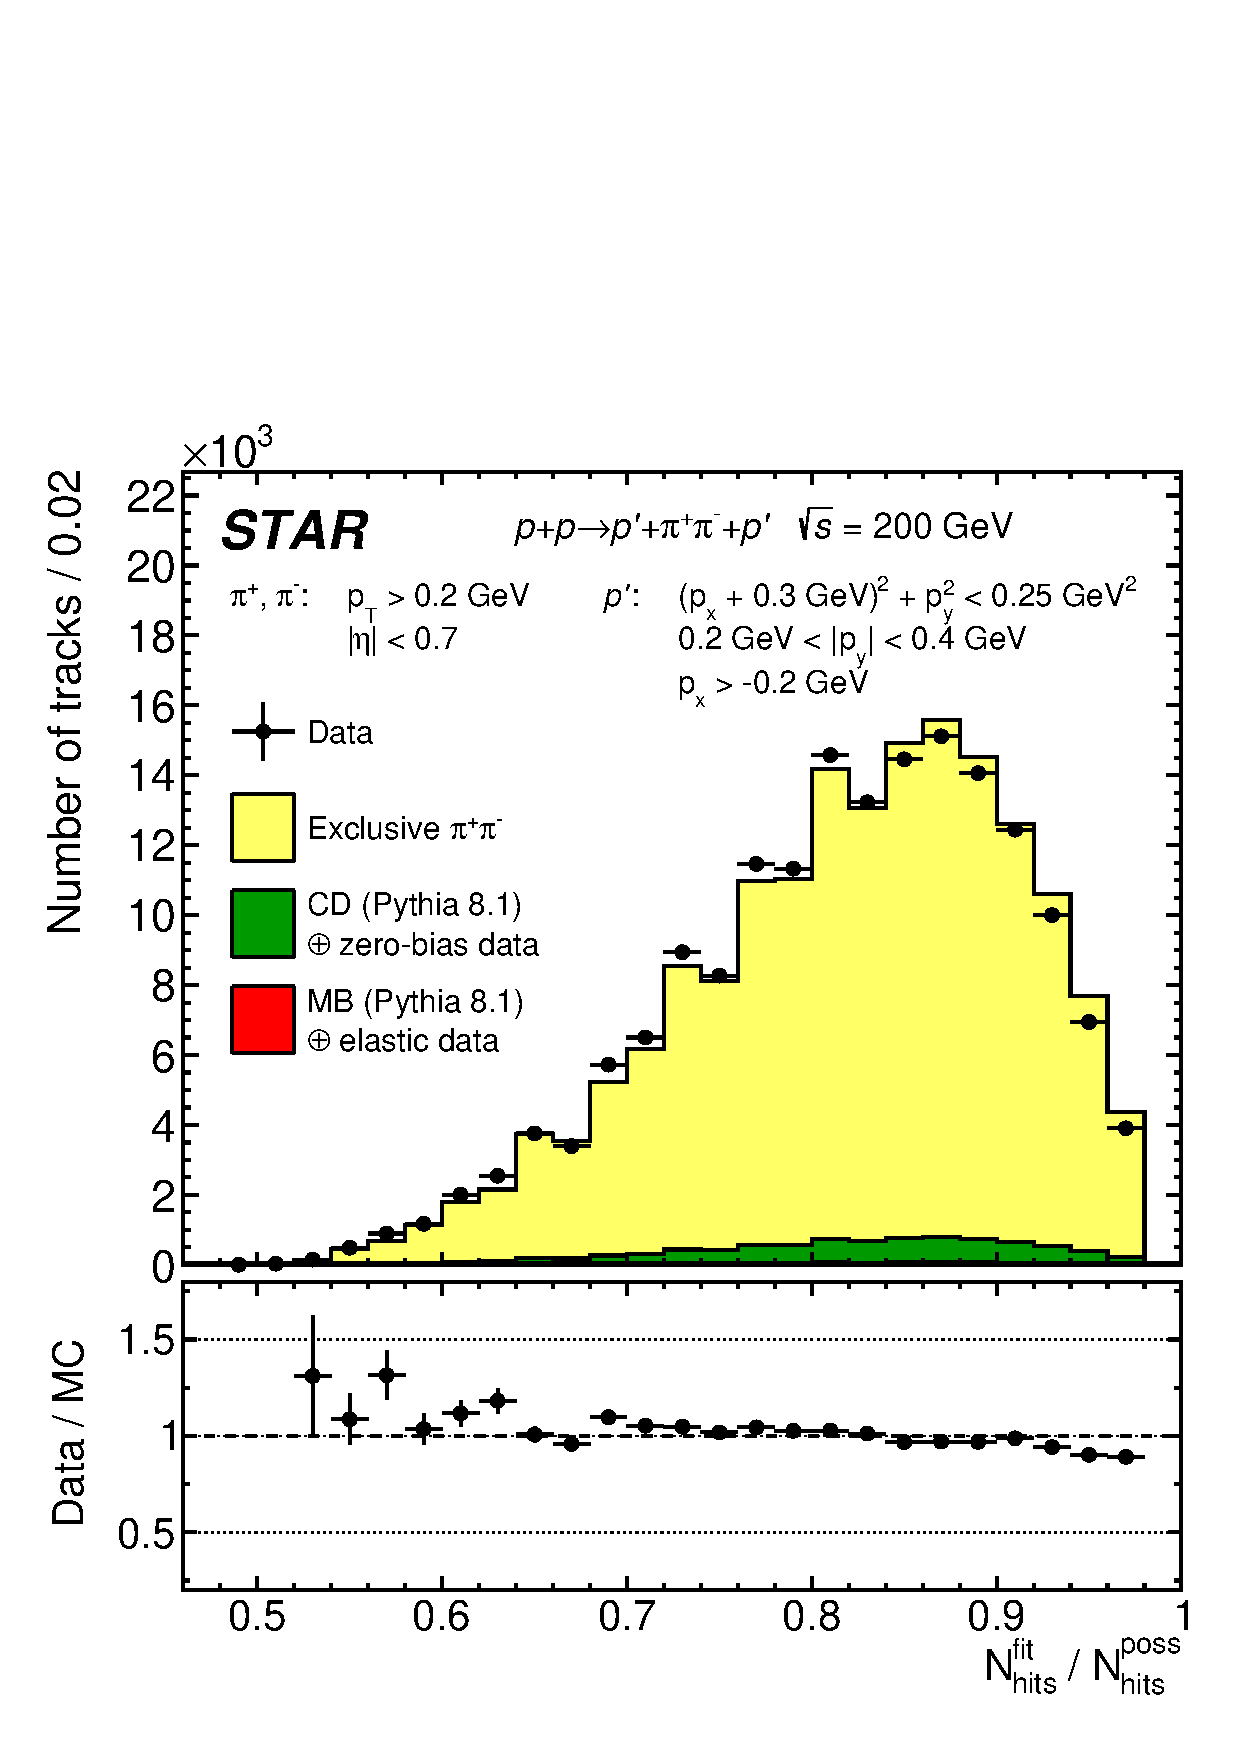
\includegraphics[width=\linewidth]{graphics/eventSelection/TpcTracks/Ratio_Linear_NHitsFit_to_NHitsPoss.pdf}}
  \end{subfigure}
}%
\quad\quad%
\parbox{0.4725\textwidth}{
  \centering
  \begin{subfigure}[b]{\linewidth}\addtocounter{subfigure}{-2}\vspace*{-23pt}
                \subcaptionbox{\label{fig:NHits_dEdx}}{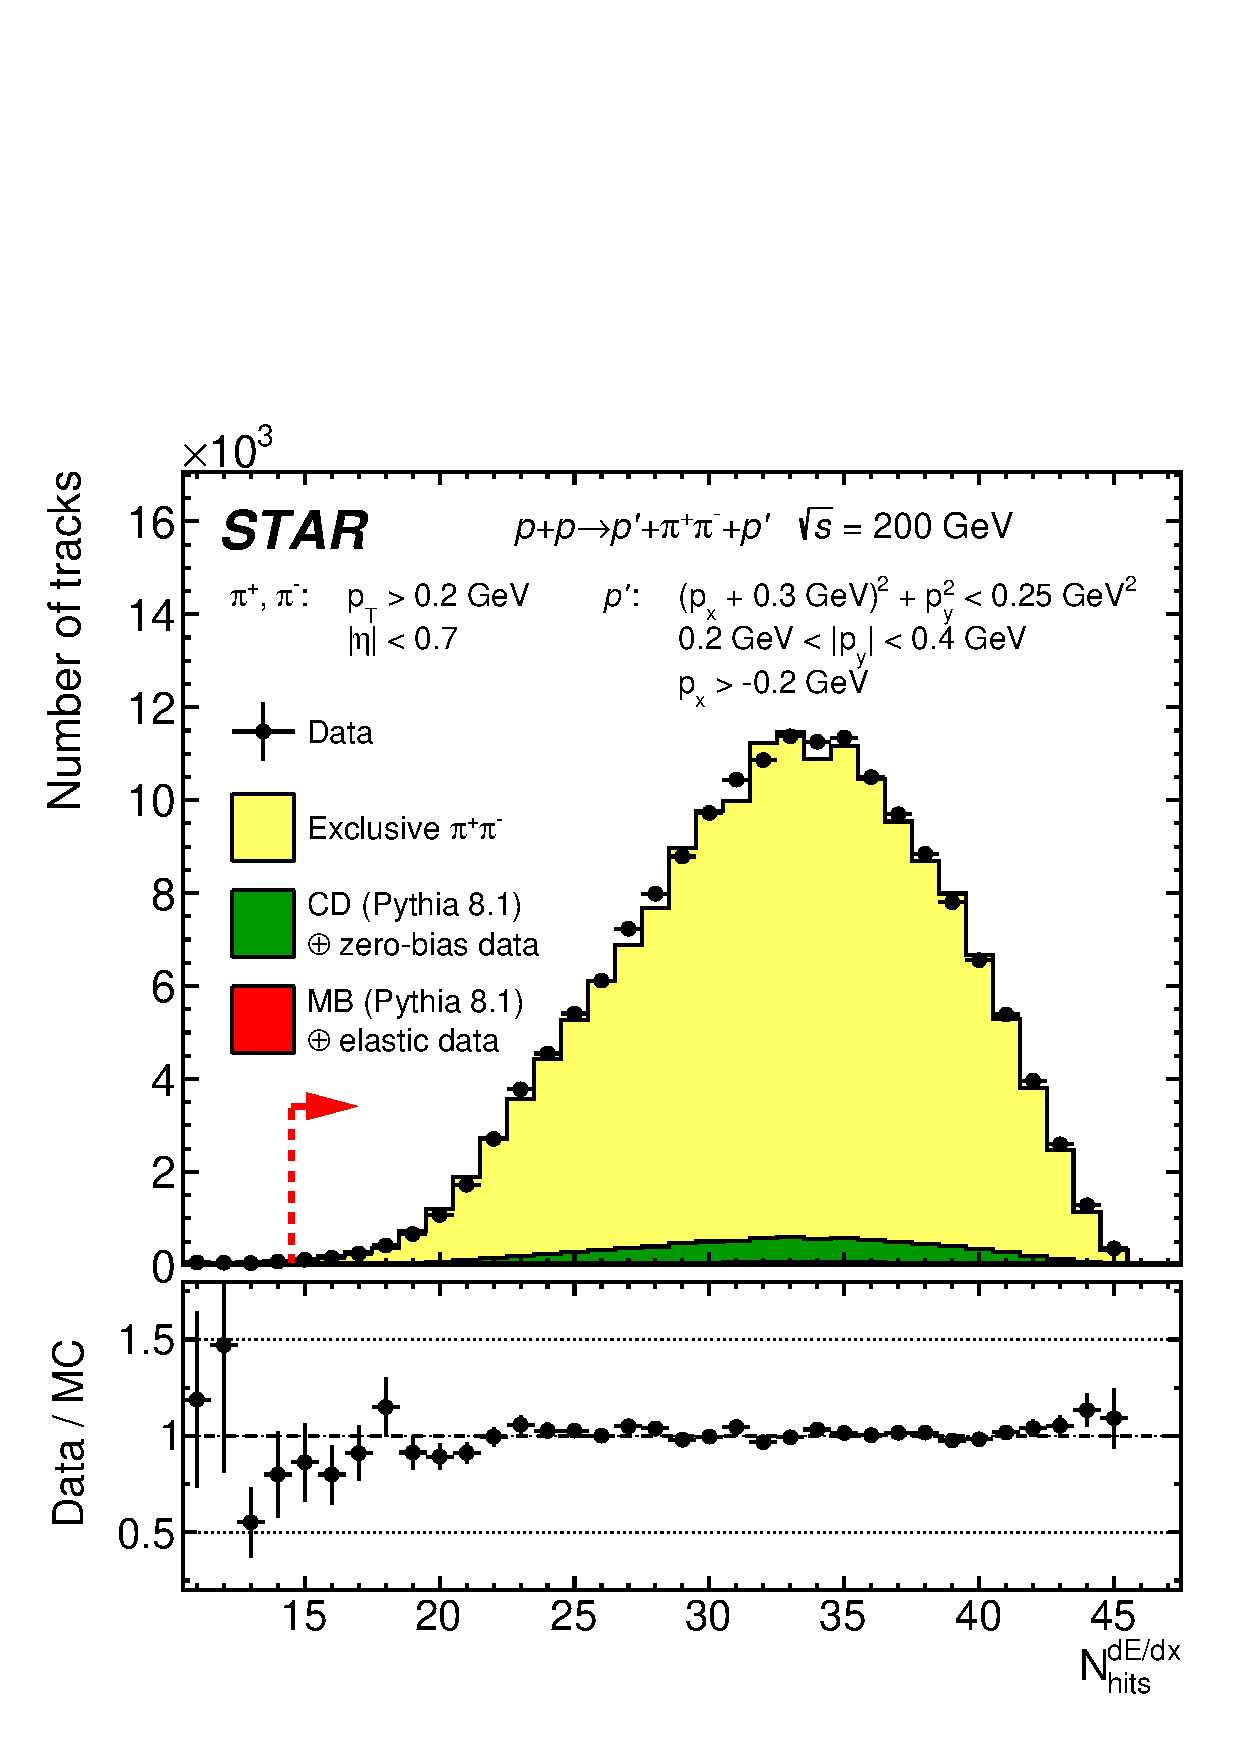
\includegraphics[width=\linewidth]{graphics/eventSelection/TpcTracks/Ratio_Linear_NHitsDEdx.pdf}}
  \end{subfigure}\\
  \begin{minipage}[t][1.042\linewidth][t]{\linewidth}\vspace{10pt}
    \caption[Comparison of distribution of $N_{\text{hits}}^{\text{fit}}$,~$N_{\text{hits}}^{\text{dE/dx}}$ and $N_{\text{hits}}^{\text{fit}}/N_{\text{hits}}^{\text{poss}}$ in the data and embedded MC.]
    {Comparison of distribution of the number of hits used in TPC track reconstruction $N_{\text{hits}}^{\text{fit}}$ (\subref{fig:NHitsFit}), number of hits used in specific energy loss reconstruction $N_{\text{hits}}^{\text{dE/dx}}$ (\subref{fig:NHits_dEdx}) and fraction of number of hits potentially generated by the track and finally used in the reconstruction $N_{\text{hits}}^{\text{fit}}/N_{\text{hits}}^{\text{poss}}$ (\subref{fig:NHitsFit_to_NHitsPos}) in the data (black points) and embedded MC (stacked color histograms). Normalizations of the signal and backgrounds were established according to description in Sec.~\ref{sec:bkgdSignalNorm}. Predictions for MCs other than GenEx (yellow) were replaced by predictions for GenEx scaled to have the same integrals as replaced histograms - this was driven by the fact that only GenEx was embedded into zero-bias TPC data, which is required to describe the three presented quantities. Vertical error bars represent statistical uncertainties, horizontal bars represent bin sizes. Red dashed line and red arrow indicate the range of each quantity which is accepted in analysis (if cut on this quantity is applied).}\label{fig:NHits}
  \end{minipage}
}%

\end{figure}
%---------------------------






%---------------------------
\begin{figure}[ht!]
\centering
\parbox{0.4725\textwidth}{
  \centering
  \begin{subfigure}[b]{\linewidth}{
                \subcaptionbox{\label{fig:TrackEta}}{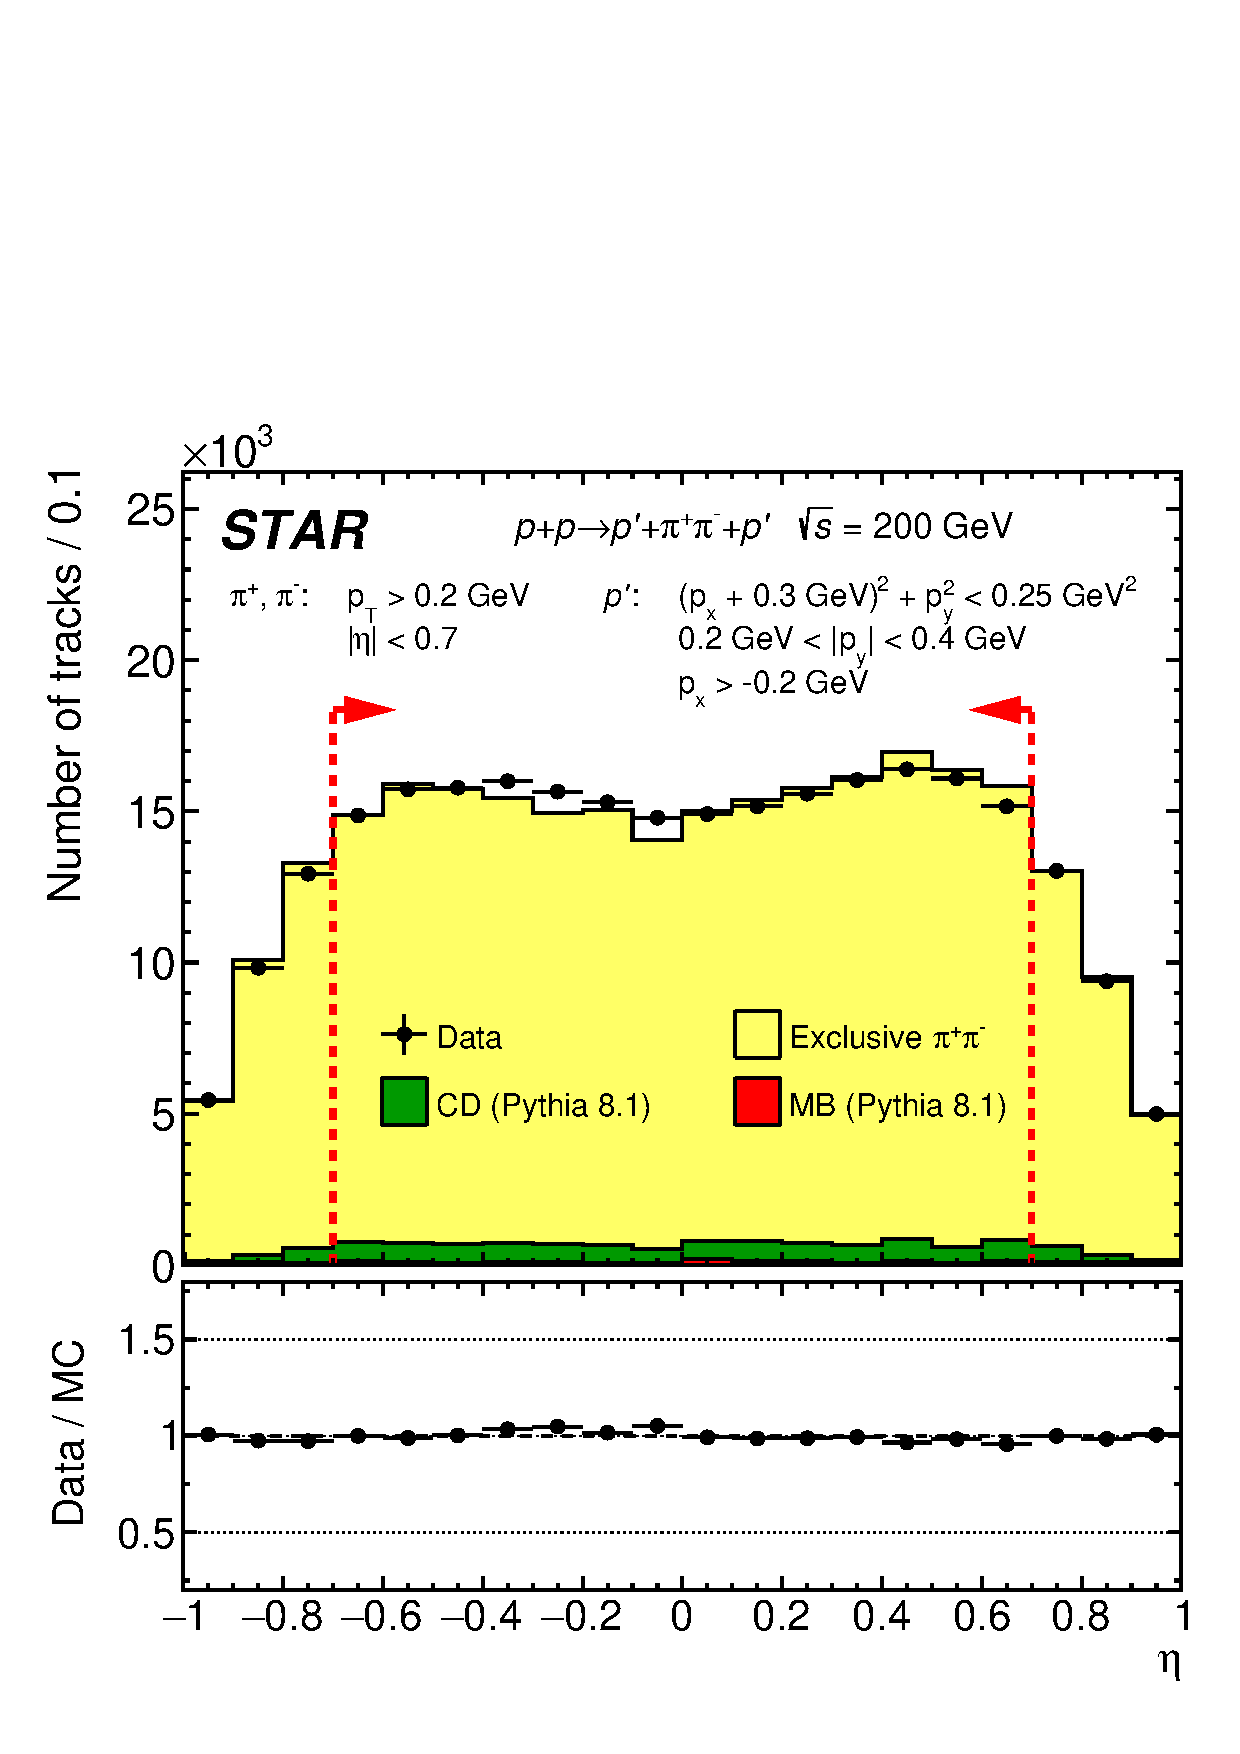
\includegraphics[width=\linewidth]{graphics/eventSelection/TpcTracks/Ratio_Linear_Eta.pdf}}}
  \end{subfigure}
}%
\quad\quad%
\parbox{0.4725\textwidth}{%
  \centering
  \begin{subfigure}[b]{\linewidth}{
                \subcaptionbox{\label{fig:TrackPhi}}{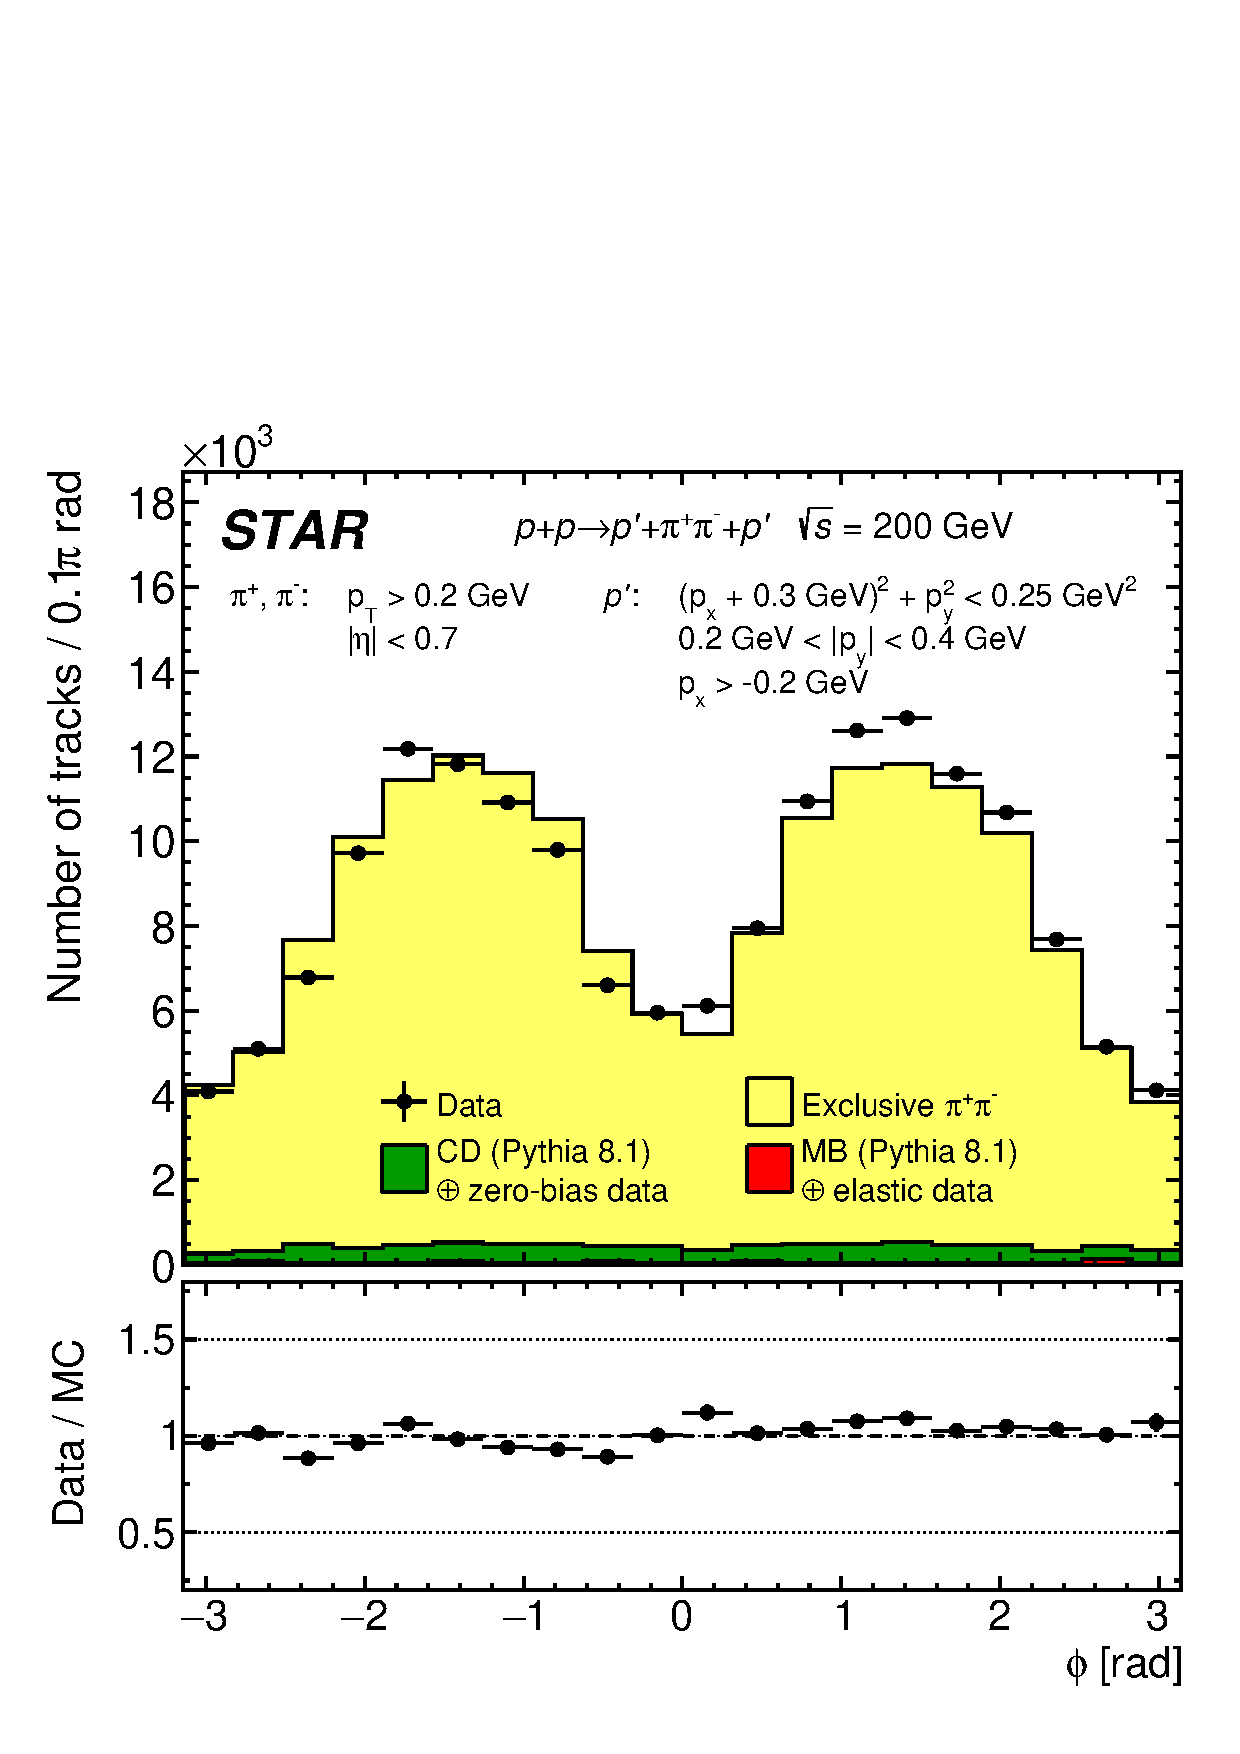
\includegraphics[width=\linewidth]{graphics/eventSelection/TpcTracks/Ratio_Linear_Phi.pdf}}}
  \end{subfigure}
}%1
\caption[Comparison of distribution of track $\eta$ and $\phi$ in the data and embedded MC.]
{Comparison of the track pseudorapidity $\eta$ (\subref{fig:TrackEta}) and the track azimuthal angle $\phi$ (\subref{fig:TrackPhi}) in the data (black points) and embedded MC (stacked color histograms). Normalizations of the signal and backgrounds were established according to description in Sec.~\ref{sec:bkgdSignalNorm}. Vertical error bars represent statistical uncertainties, horizontal bars represent bin sizes. Red dashed line and red arrow indicate the range of each quantity which is accepted in analysis (if cut on this quantity is applied).}\label{fig:TrackEtaPhi}
\end{figure}
%---------------------------









\subsection{(\ref{enum:CutRpTrks})~RP tracks}\label{sec:C4}

In presented physics analysis highest-level forward objects were used - the RP tracks. They are obtained through the reconstruction starting from the signals in single channels of silicon strip detectors housed inside RPs. General description of the reconstruction procedure has been given in Sec.~6.2 of the supplementary analysis note~\cite{supplementaryNote} and reference therein. A bit more detail description is available in elastic proton-proton scattering measurement note~\cite{elasticNote}.


Roman Pot data was analyzed offline as follows. First, all RP tracks which contain track points that had been formed of less than 3 hits of out 4 maximally possible (1 hit per silicon plane), were rejected. This is natural consequence of very high single plane efficiency $>99.5\%$, and prevents including to analysis tracks with track points formed from unmatched pairs of clusters in both $x$- and $y$-coordinate (e.g. from electronics noise).

%---------------------------
\begin{figure}[b!]
\centering
\parbox{0.4725\textwidth}{
  \centering
  \begin{subfigure}[b]{\linewidth}
                \subcaptionbox{\label{fig:localAngle2D_X}}{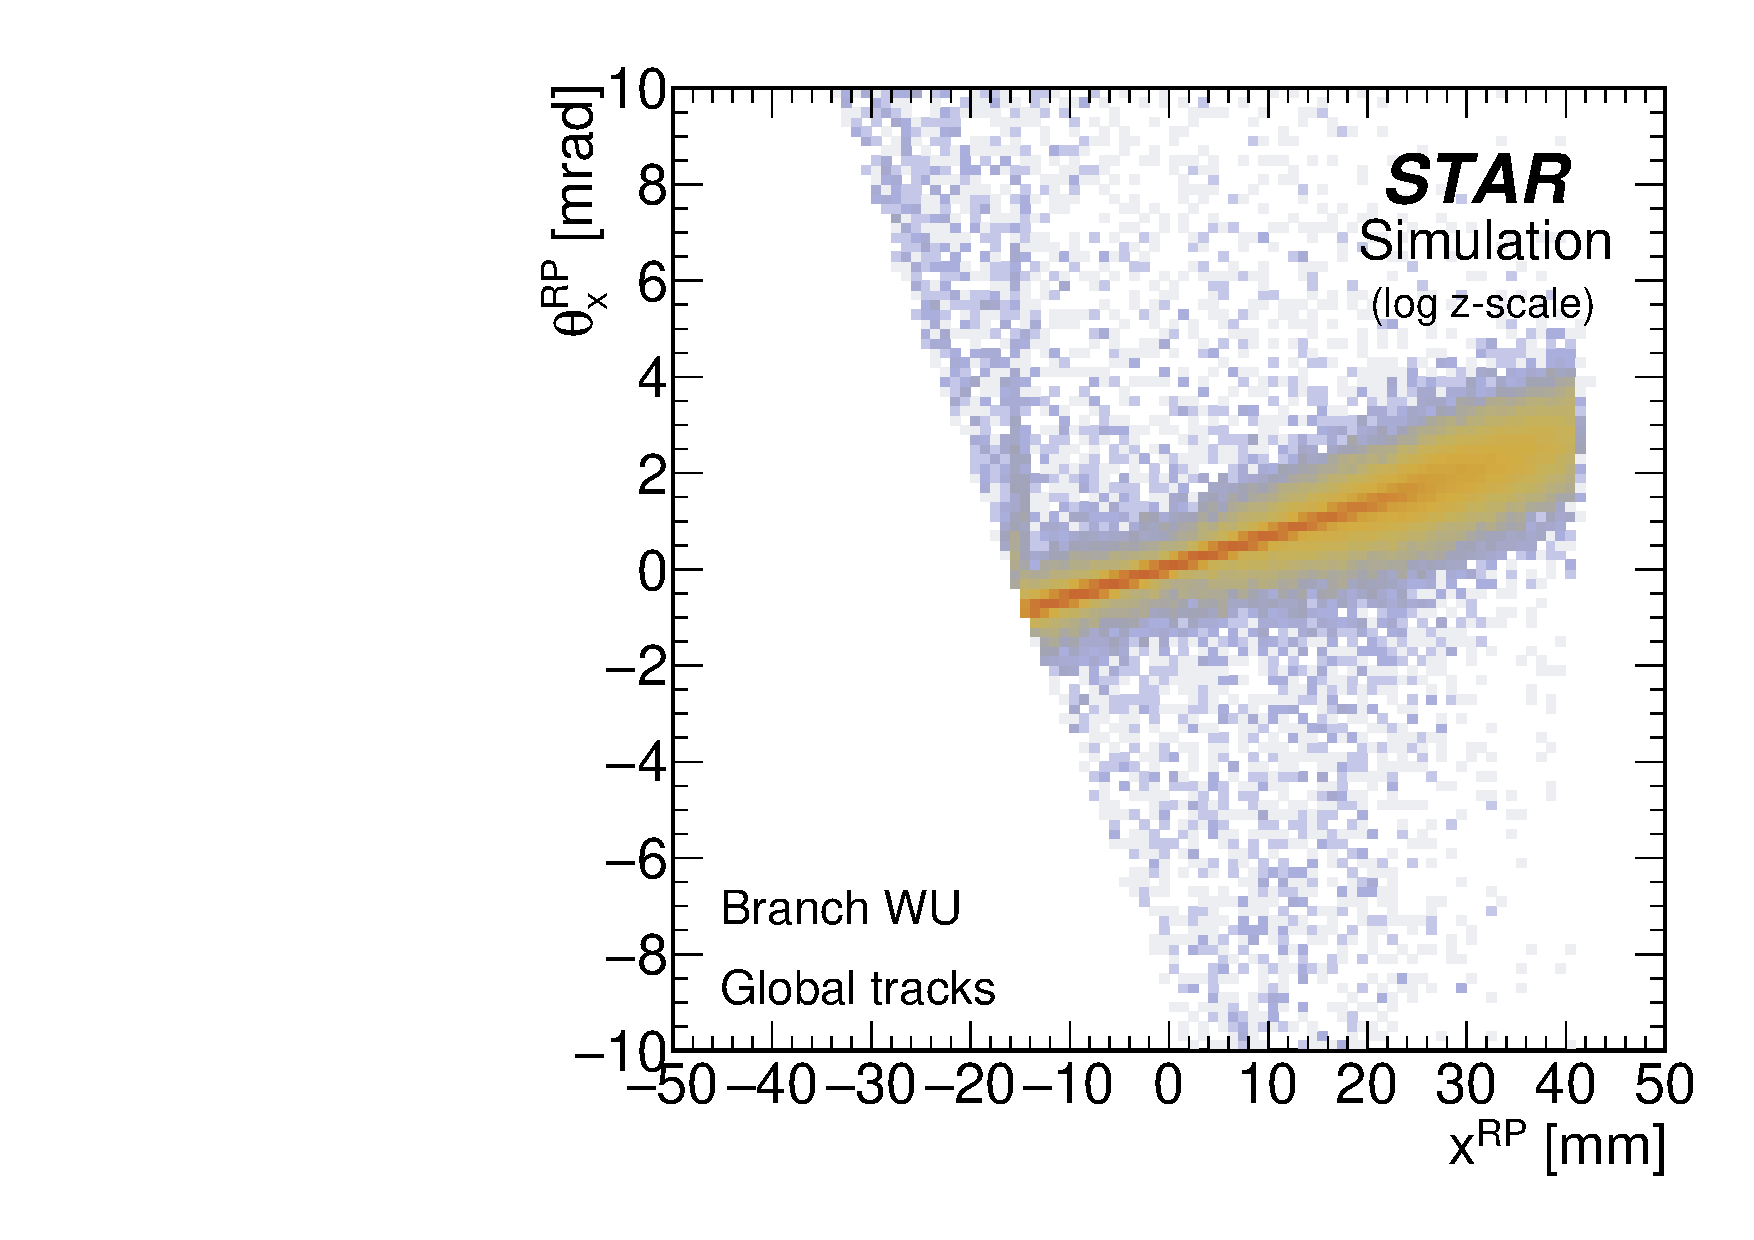
\includegraphics[width=\linewidth,page=1]{graphics/eventSelection/RpTracks/RpTrackCuts_2.pdf}\vspace*{-10pt}}
  \end{subfigure}\\
  \begin{subfigure}[b]{\linewidth}\addtocounter{subfigure}{1}
                \subcaptionbox{\label{fig:localAngle1D_X}}{\includegraphics[width=\linewidth,page=2]{graphics/eventSelection/RpTracks/RpTrackCuts_2.pdf}}
  \end{subfigure}
}%
\quad\quad%
\parbox{0.4725\textwidth}{
  \centering
  \begin{subfigure}[b]{\linewidth}\addtocounter{subfigure}{-2}
                \subcaptionbox{\label{fig:localAngle2D_Y}}{\includegraphics[width=\linewidth,page=3]{graphics/eventSelection/RpTracks/RpTrackCuts_2.pdf}\vspace*{-10pt}}
  \end{subfigure}\\
  \begin{subfigure}[b]{\linewidth}\addtocounter{subfigure}{1}
                \subcaptionbox{\label{fig:localAngle1D_Y}}{\includegraphics[width=\linewidth,page=4]{graphics/eventSelection/RpTracks/RpTrackCuts_2.pdf}}
  \end{subfigure}
}%
\caption[Local angle vs. position of RP tracks matched with true level primary protons.]{Typical correlation between local angle ($y$-axis) and position ($x$-axis) of RP tracks matched with true level primary protons for $x$- (\subref{fig:localAngle2D_X}) and $y$-coordinate (\subref{fig:localAngle2D_Y}), here shown for branch WU. The same events are contained in \subref{fig:localAngle1D_X} and \subref{fig:localAngle1D_Y} for $x$- and $y$-coordinate respectively, where difference between reconstructed local angle and local angle expected from the elastic track is histogrammed. Red lines and arrows visualize cuts imposed on RP tracks for final selection (cuts~\ref{enum:RpLocalAngles}).}\label{fig:localAngleRp}%
\end{figure}
%---------------------------

Next, preselected tracks were verified for consistency of their local angles with hypothesis of their origin being at the STAR IR. Using Geant4 simulation of RP system (see Sec.~6.3. of Ref.~\cite{supplementaryNote}) the impact of apertures limiting RP acceptance for the forward scattered protons generated at STAR IR was tested. The result is shown in Fig.~\ref{fig:localAngleRp}, where density maps of reconstructed RP track local angle $\theta^{\text{RP}}$ and corresponding track coordinate in RP station are drawn (we show it only for branch WU as the picture is the same in the remaing branches). Only RP tracks matched with generated primary forward protons were used to fill the histograms. Clear bands of primary proton tracks can be distinguished in the top plots (Figs.~\ref{fig:localAngle2D_X} and~\ref{fig:localAngle2D_Y}), with some very small number of tracks significantly scattered on the beampipe/DX/detector material. One-dimensional representation of the correlation between local angle and position can be obtained by constructing quantities
\begin{equation}
 \widetilde{\Delta}\theta_{x}^{RP} = \theta_{x}^{\text{RP}}-x^{\text{RP}}/|z^{\text{RP}}|,
\end{equation}
\begin{equation}
 \widetilde{\Delta}\theta_{y}^{RP} = \theta_{y}^{\text{RP}}-y^{\text{RP}}/|z^{\text{RP}}|,
\end{equation}%
which reflect deviation of reconstructed local angle from expectation for forward proton of the beam momentum, and whose distributions are presented in Fig.~\ref{fig:localAngle1D_X} and Fig.~\ref{fig:localAngle1D_Y}, respectively (black histograms). On these one-dimensional histograms we clearly see peaks from the true primary tracks. We considered optimal to restrict accepted $\widetilde{\Delta}\theta_{x}^{RP}$ from -2~mrad to 4~mrad, and $\widetilde{\Delta}\theta_{y}^{RP}$ from -2~mrad to 2~mrad. The upper cut on $\widetilde{\Delta}\theta_{x}^{RP}$ equal to  4~mrad may look too inclusive, but intention was to preserve tracks of protons with very large $\xi$, whose local angle highly deviates from that of elastically scattered protons (DX magnets bends more protons with lower momentum) and which might have been underpopulated in MC (GenEx predictions were used). It is also worth to comment on the blue histograms in Figs.~\ref{fig:localAngle1D_X} and~\ref{fig:localAngle1D_Y}, which represent local tracks (formed of single track points). These tracks are reconstructed assuming their momentum is equal to the beam momentum (angle at vertex equal to angle at RP station), therefore $\widetilde{\Delta}\theta_{x}^{RP}$ and $\widetilde{\Delta}\theta_{y}^{RP}$ is 0 by definition.


Once the set of cuts above was applied we required that on each side of STAR there was exactly one selected RP track. We did not allow higher number of tracks on one side because of no clear way to discriminate real tracks of primary protons.

In addition to cuts above, we restricted our measurement to the fiducial region defined as
\begin{equation}\label{eq:RpFiducial}
0.2<|p_{y}|<0.4,~~~-0.2<p_{x},~~~(p_{x}+0.3)^{2}+p_{y}^{2}<0.5^{2}~~~(\text{all in GeV}), 
\end{equation}
therefore both RP tracks were required to be contained within above envelope in $(p_{x}, p_{y})$ space. This fiducial area is drawn with black solid line on top of the $(p_{x}, p_{y})$ distribution of all measured CEP candidates (Fig.~\ref{fig:rp_hits}). It was chosen to compromize signal statistics and systematic uncertainties of the RP-related efficiencies (see e.g. Sec.~10.3 of Ref.~\cite{supplementaryNote}).

\begin{figure}[b!]
\centering
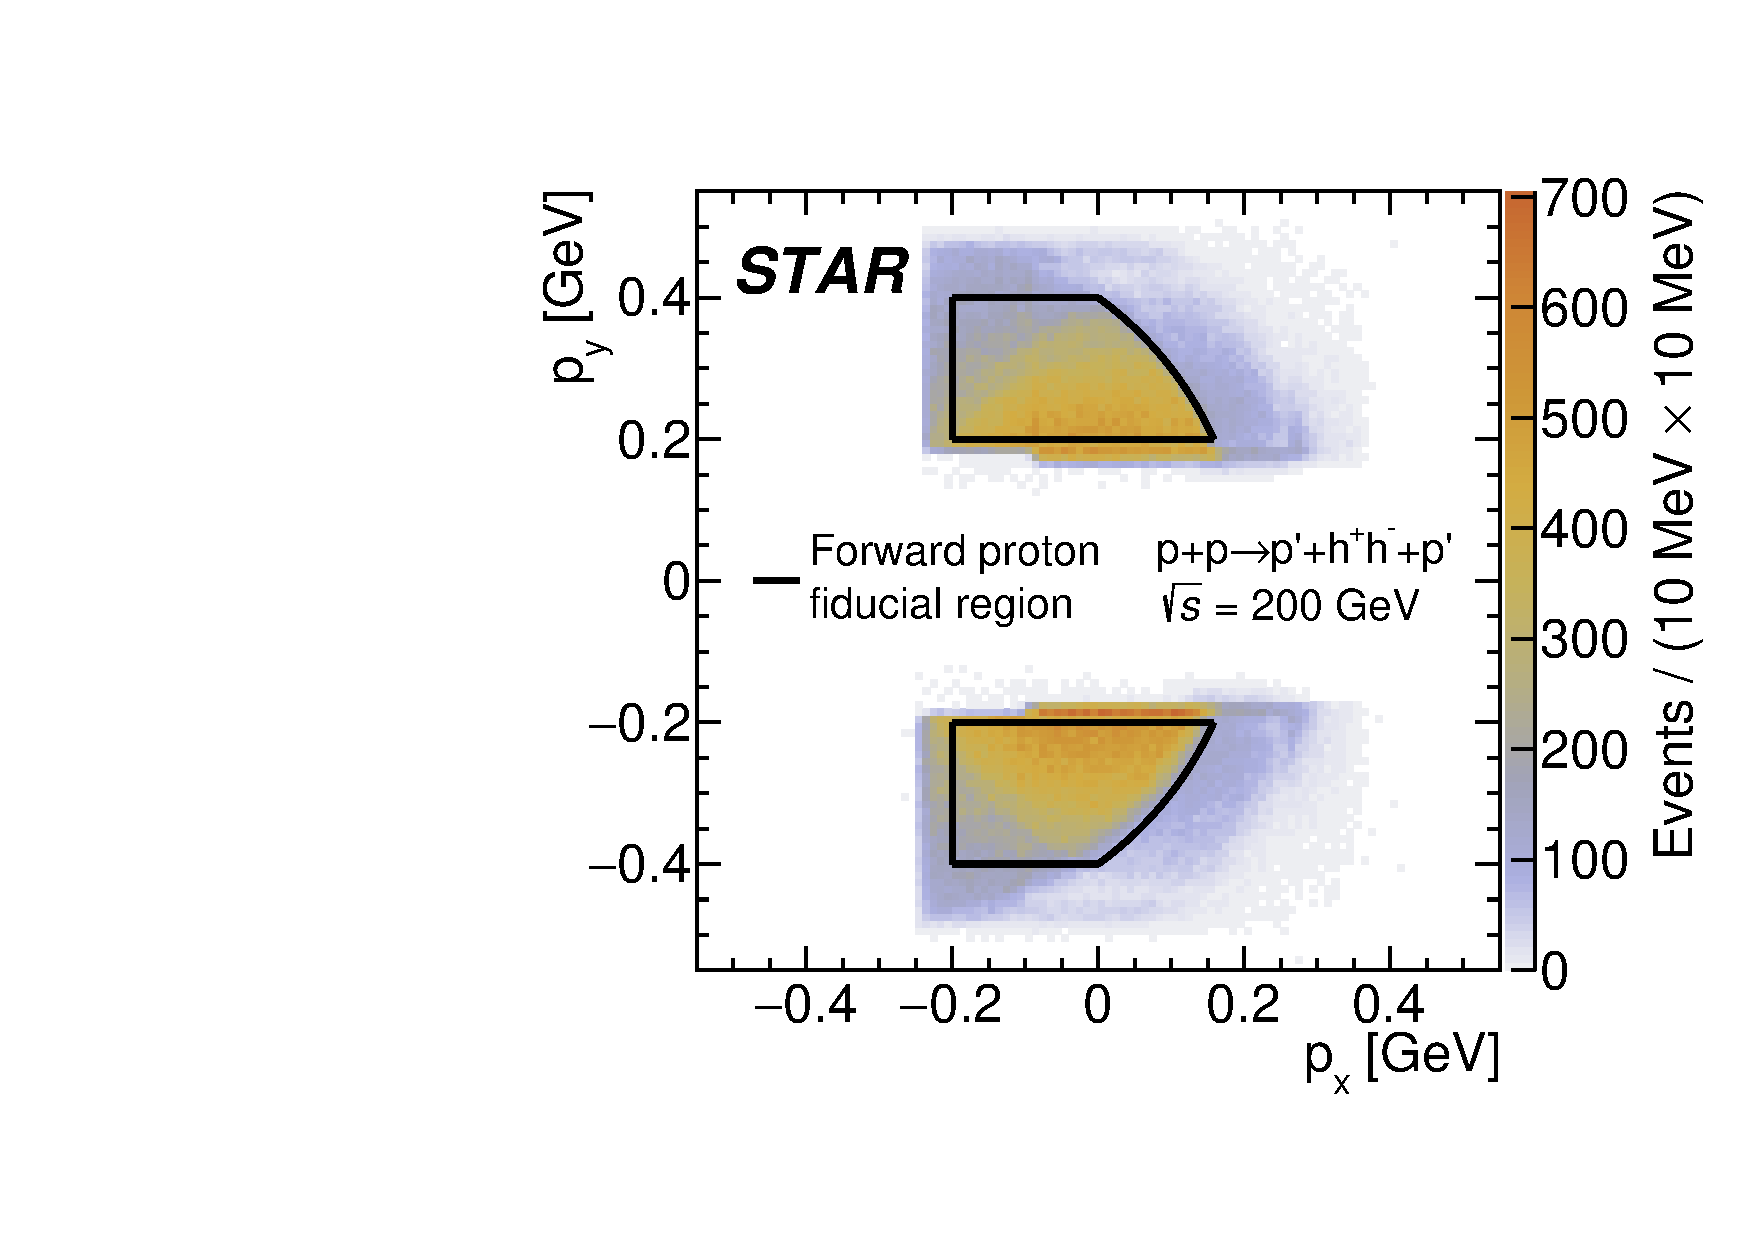
\includegraphics[width=.465\textwidth]{graphics/eventSelection/RpTracks/PxPyExclusiveAllMerged.pdf}
%\hfill
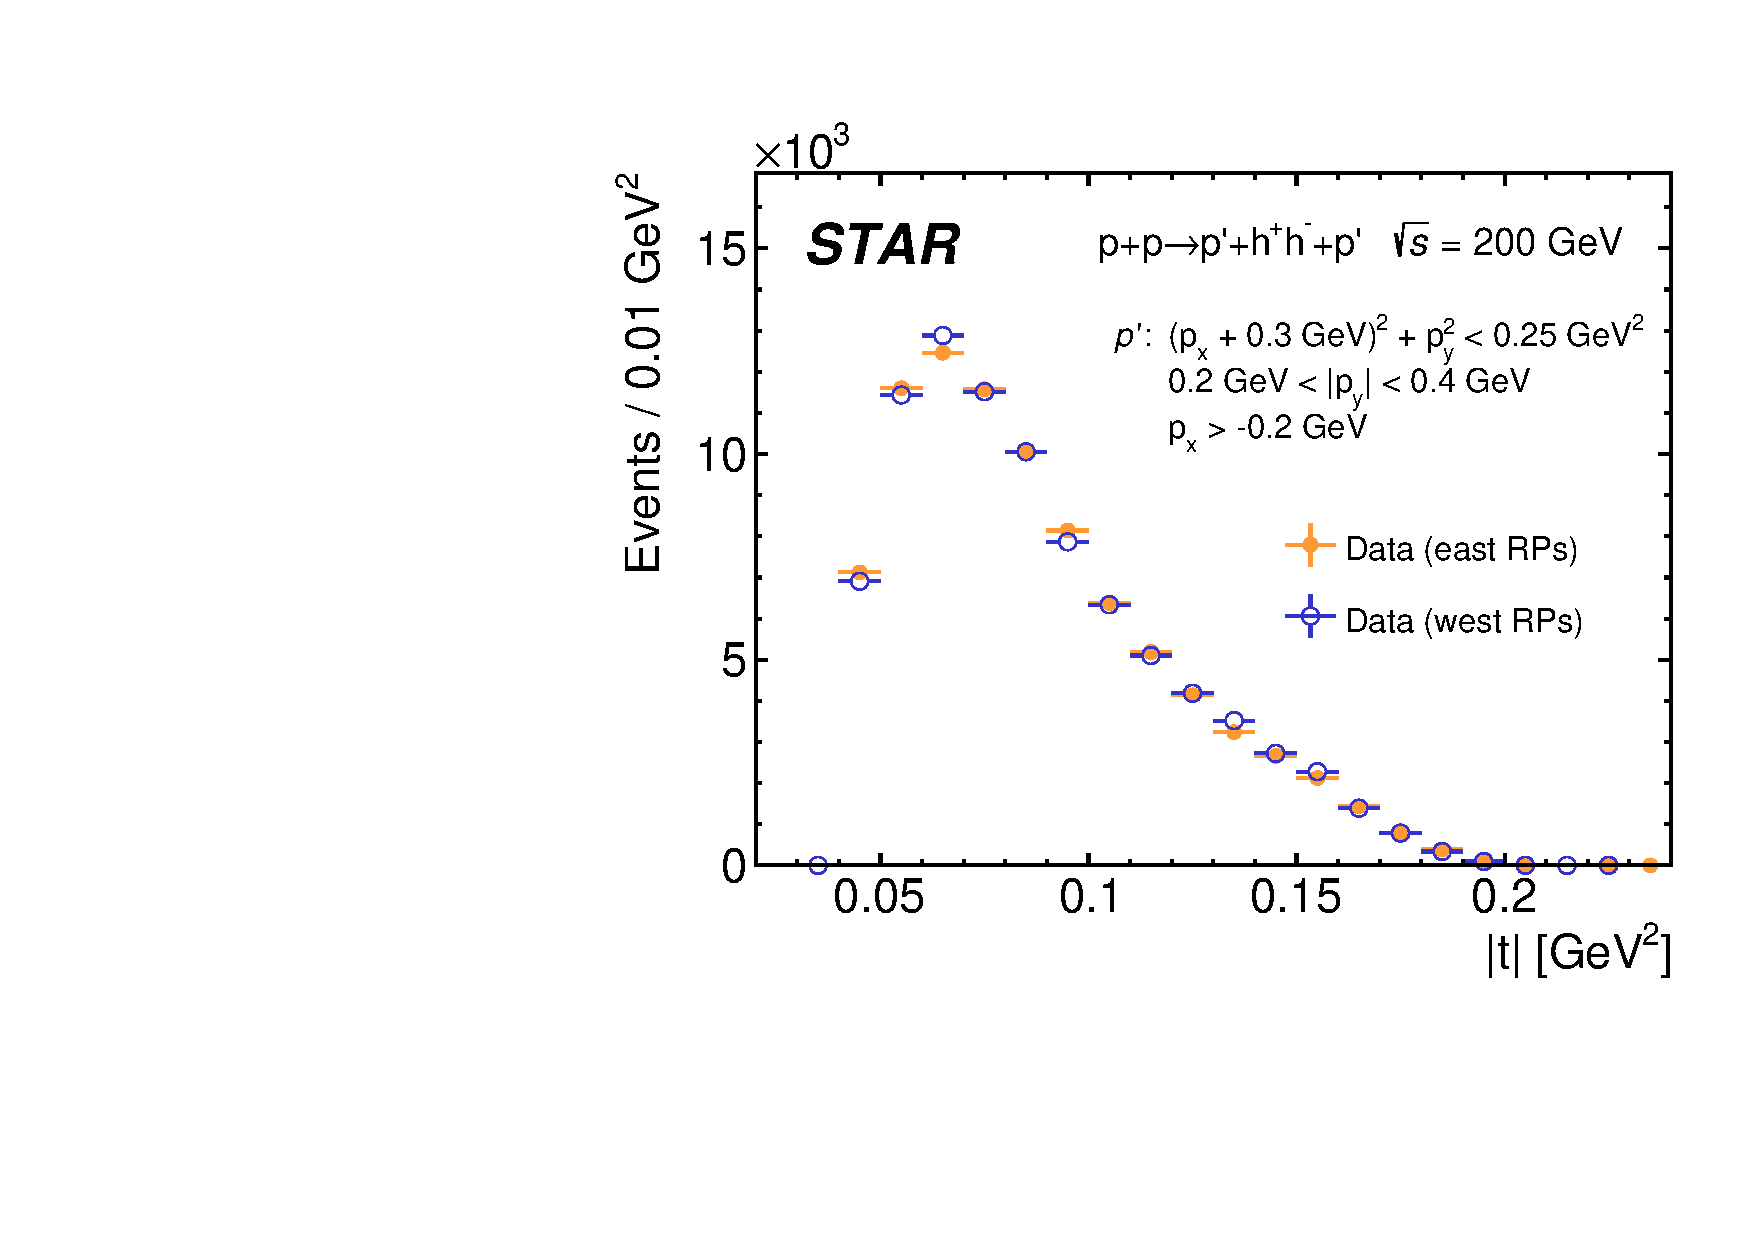
\includegraphics[width=.523\textwidth]{graphics/eventSelection/RpTracks/Paper_MandelstamT.pdf}
%
\caption{(left) Merged distributions of diffractively scattered protons momenta $p_y$ vs. $p_x$ in exclusive $h^{+}h^{-}$ events reconstructed with the East and West RP stations, together with the kinematic region used in the measurement marked with the black line. (right) Distributions of measured four momenta transfers at the proton vertices for exclusive $h^{+}h^{-}$ events with all particles in the fiducial phase space are shown for East and West stations with yellow and blue color, respectively.}
\label{fig:rp_hits}
\end{figure}


In the remaining part of the section we show comparisons of the track points position distributions between the data and embedded MC. In Fig.~\ref{fig:hitMap_DataVsMC} we present side-by-side comparisons of two-dimensional hit maps from the data and embedded MC. Figures~\ref{fig:xRp} and~\ref{fig:yRp} show the same comparisons, but between their $x$- and $y$-projections for each RP separately. One can see, that simulation generally describes data well, both in terms of shapes (which is mainly sensitive to detector alignment and geometry/apertures) and track points normalizations in various RPs (which is mainly sensitive to reconstruction efficiency).


%---------------------------
\begin{figure}[h]
\centering
\parbox{0.4725\textwidth}{
  \centering
  \begin{subfigure}[b]{\linewidth}
                \subcaptionbox{\label{fig:E1_HitMap}}{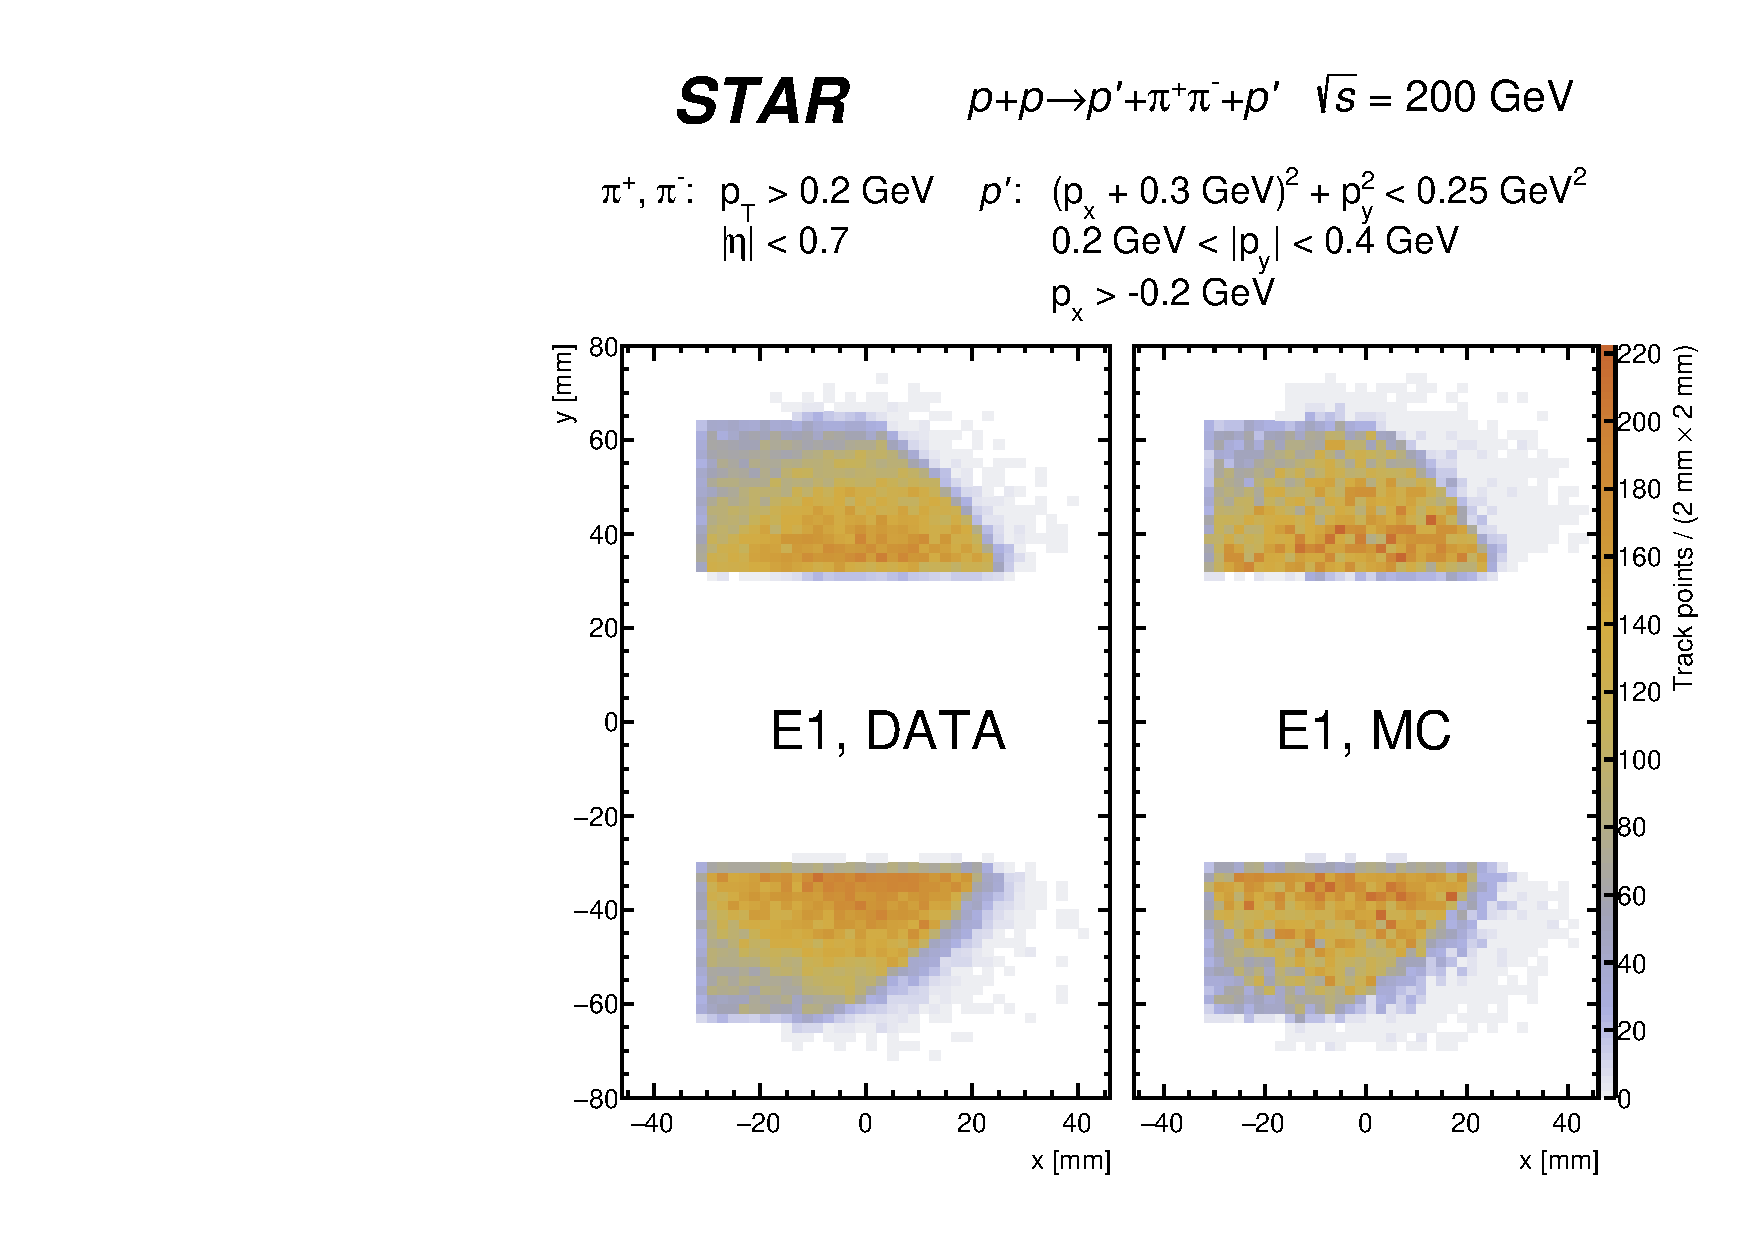
\includegraphics[width=\linewidth]{graphics/eventSelection/RpTracks/E1_HitMap.pdf}}
  \end{subfigure}\\[10pt]
  \begin{subfigure}[b]{\linewidth}\addtocounter{subfigure}{1}
                \subcaptionbox{\label{fig:W1_HitMap}}{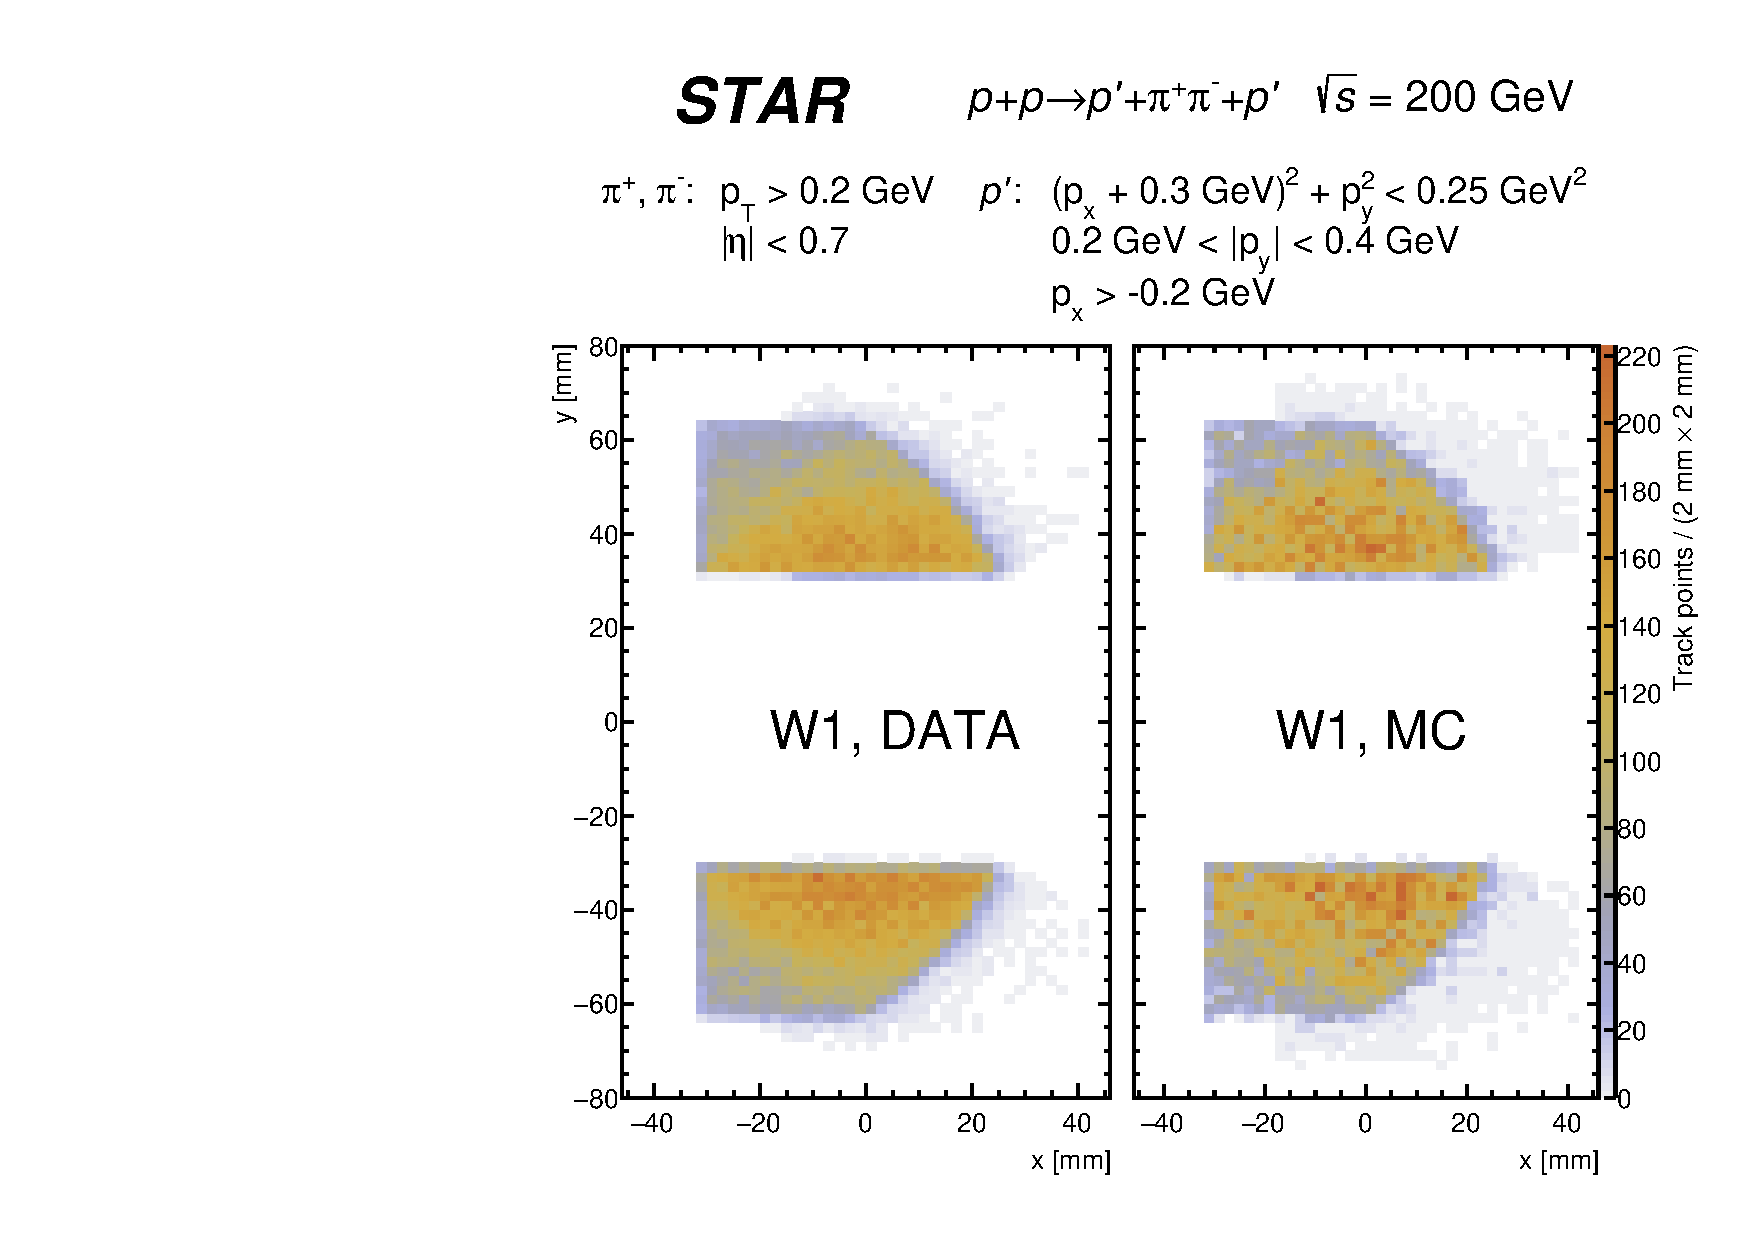
\includegraphics[width=\linewidth]{graphics/eventSelection/RpTracks/W1_HitMap.pdf}}
  \end{subfigure}
}%
\quad\quad%
\parbox{0.4725\textwidth}{
  \centering
  \begin{subfigure}[b]{\linewidth}\addtocounter{subfigure}{-2}
                \subcaptionbox{\label{fig:E2_HitMap}}{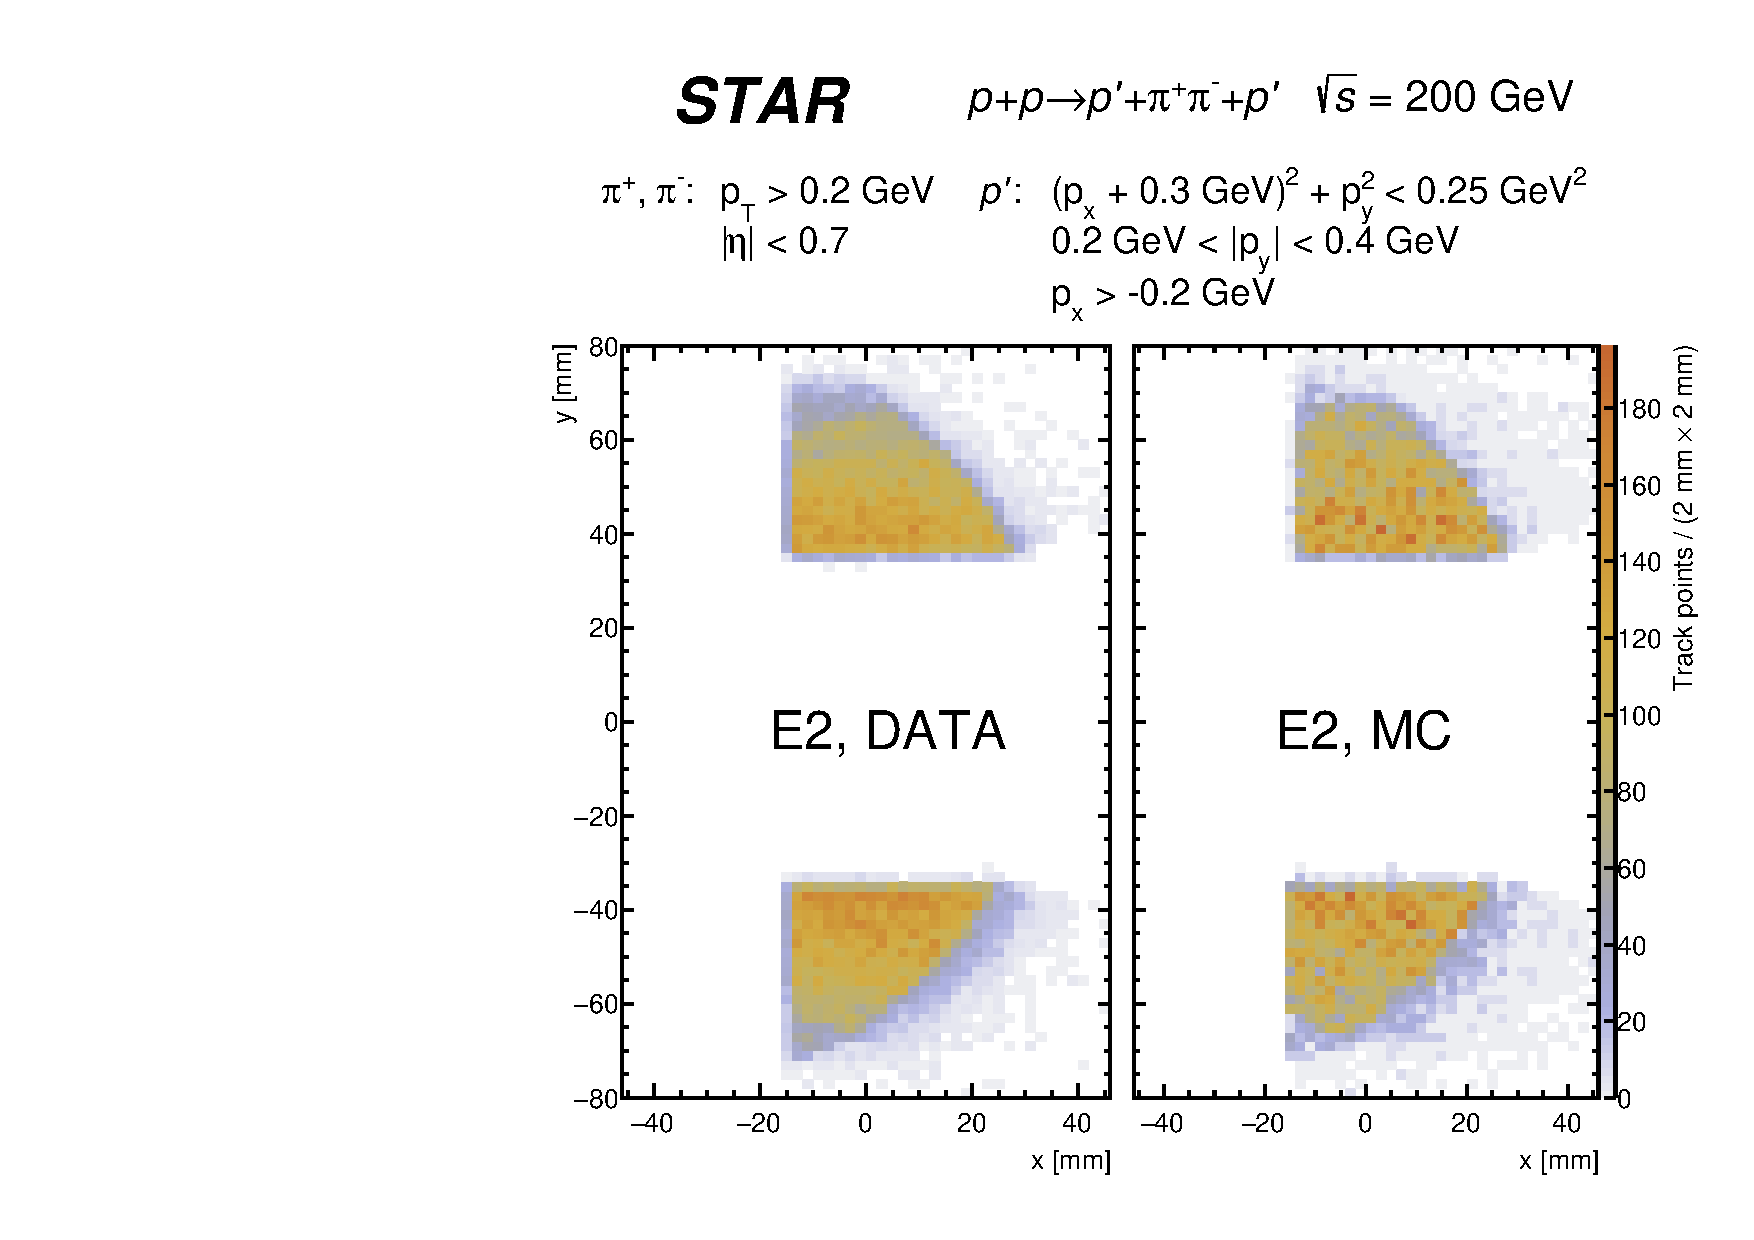
\includegraphics[width=\linewidth]{graphics/eventSelection/RpTracks/E2_HitMap.pdf}}
  \end{subfigure}\\[10pt]
  \begin{subfigure}[b]{\linewidth}\addtocounter{subfigure}{1}
                \subcaptionbox{\label{fig:W2_HitMap}}{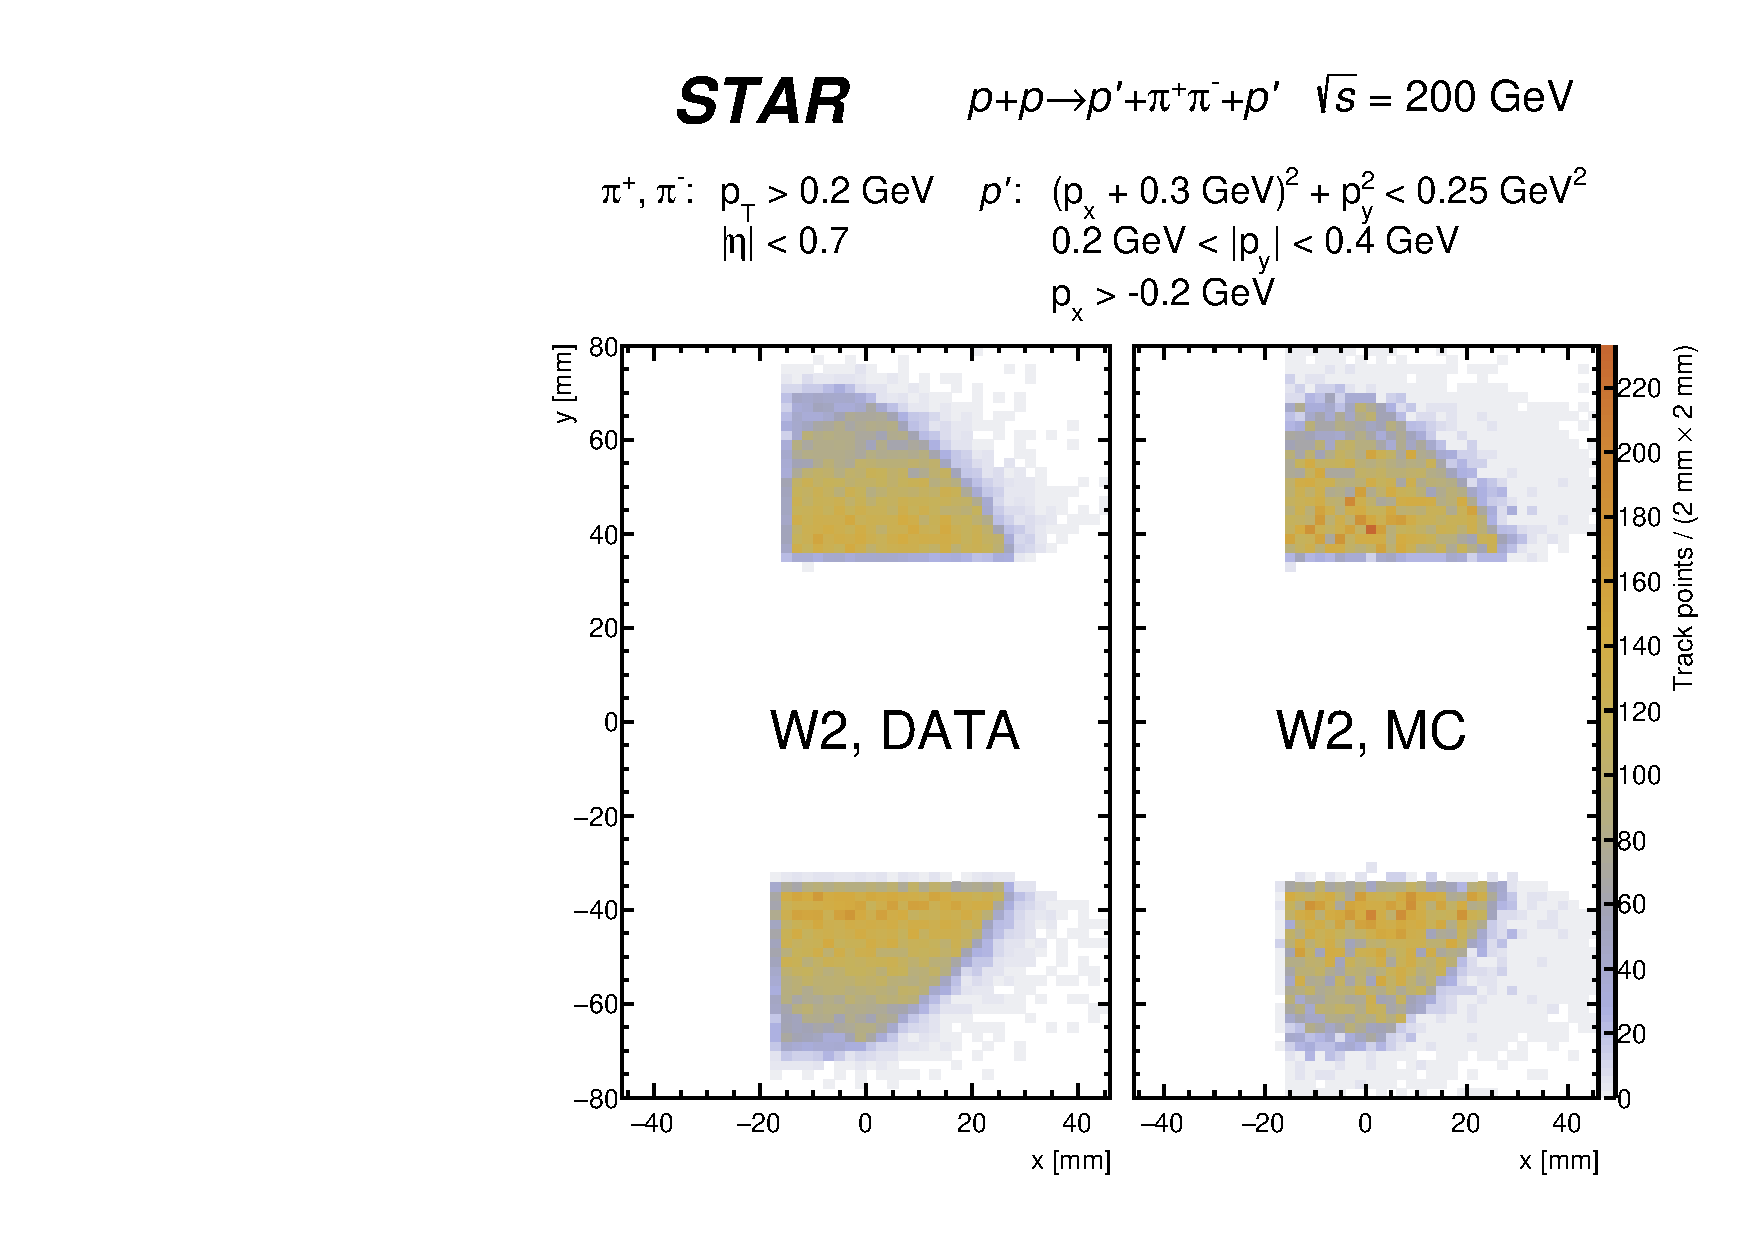
\includegraphics[width=\linewidth]{graphics/eventSelection/RpTracks/W2_HitMap.pdf}}
  \end{subfigure}
}%
\caption[Comparison of two-dimensional track point density map in the data and embedded MC.]
    {Comparison of two-dimensional track point density map in the data (left panel in subfigures) and stacked embedded MC (right panel in subfigures). Each subfigure corresponds to single RP station with position of track points measured in upper and lower RP visible at positive and negative $y$, respectively. Normalizations of the signal and backgrounds were established according to description in Sec.~\ref{sec:bkgdSignalNorm}.}\label{fig:hitMap_DataVsMC}%
\end{figure}
%---------------------------


%---------------------------
\begin{figure}[h]
\centering
\parbox{0.31\textwidth}{
  \centering
  \begin{subfigure}[b]{\linewidth}
                \subcaptionbox{\label{fig:Ratio_Linear_x_E1U}}{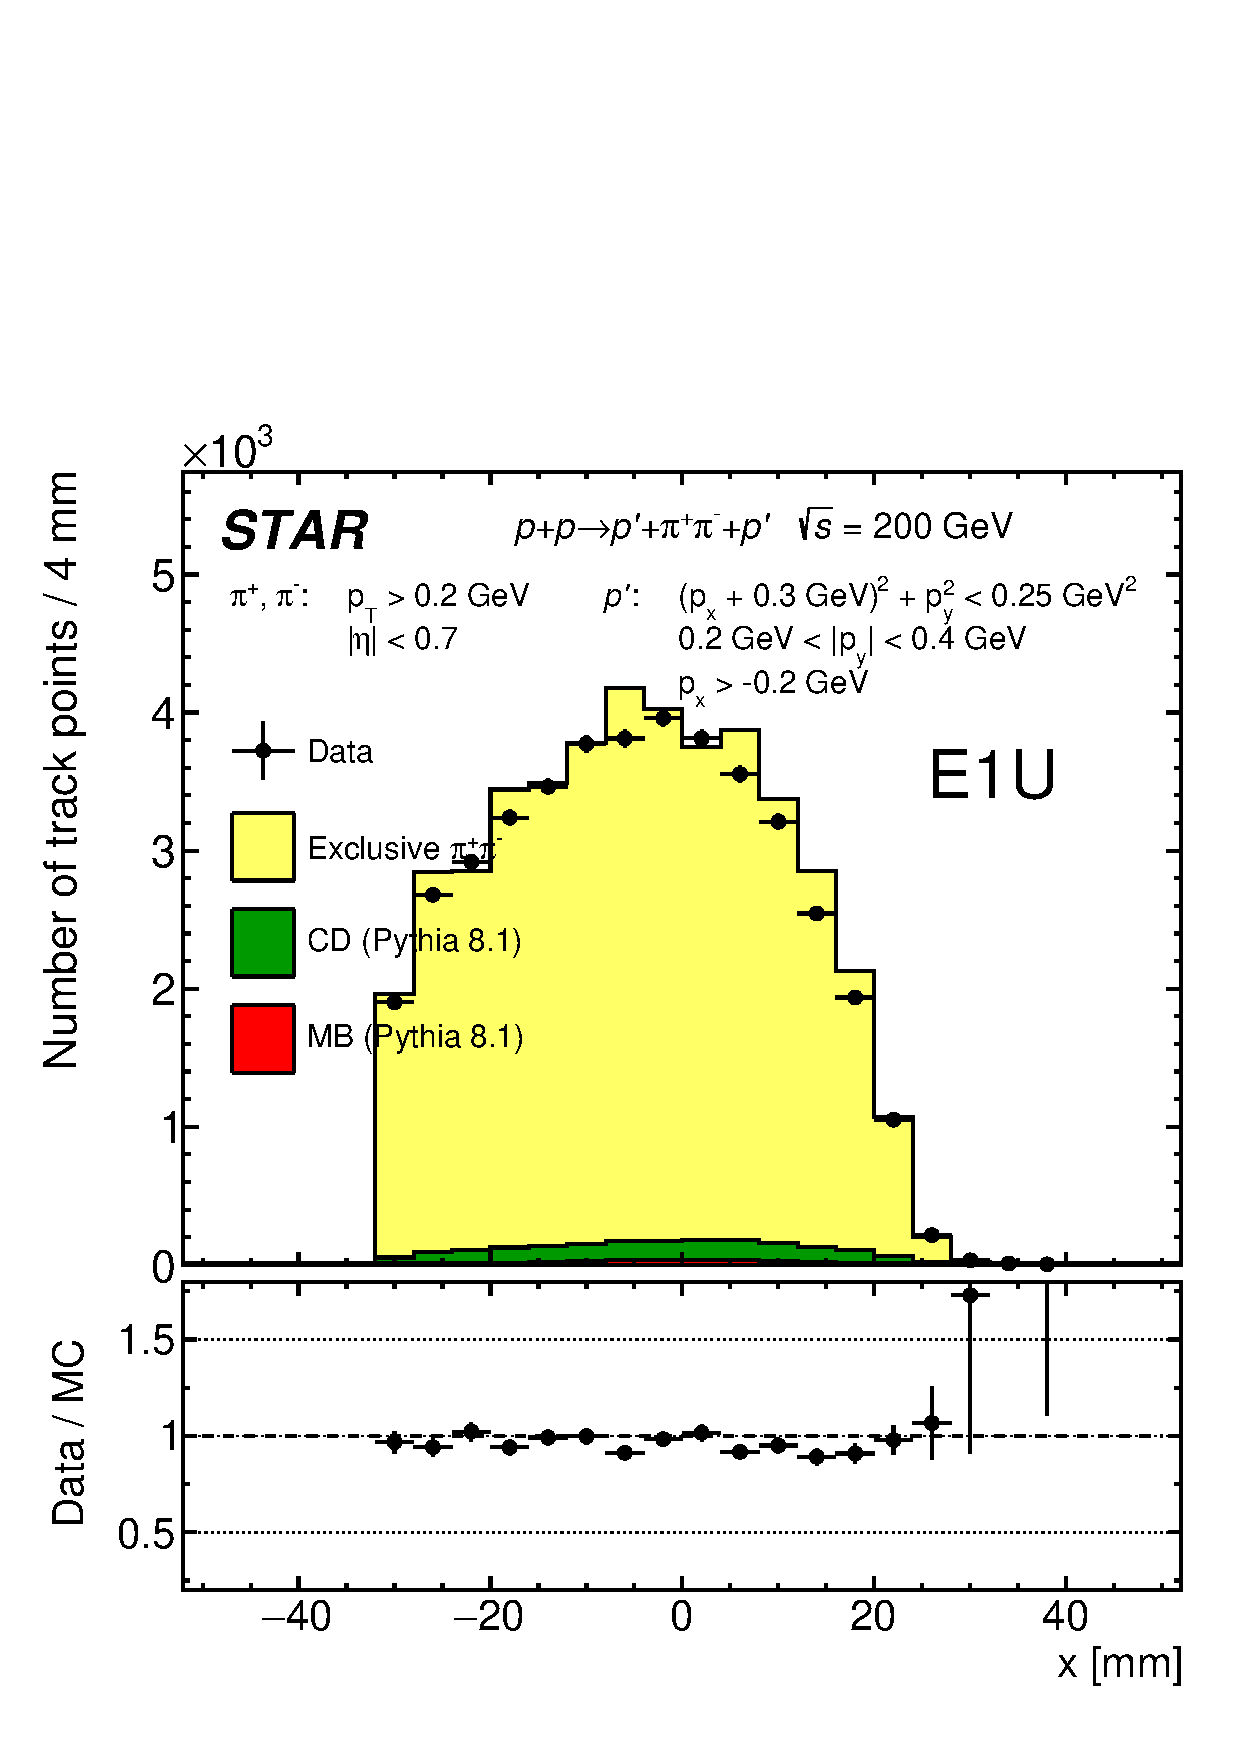
\includegraphics[width=\linewidth]{graphics/eventSelection/RpTracks/Ratio_Linear_x_E1U.pdf}\vspace*{-10pt}}
  \end{subfigure}\\[5pt]
  \begin{subfigure}[b]{\linewidth}%\addtocounter{subfigure}{1}
                \subcaptionbox{\label{fig:Ratio_Linear_x_W2U}}{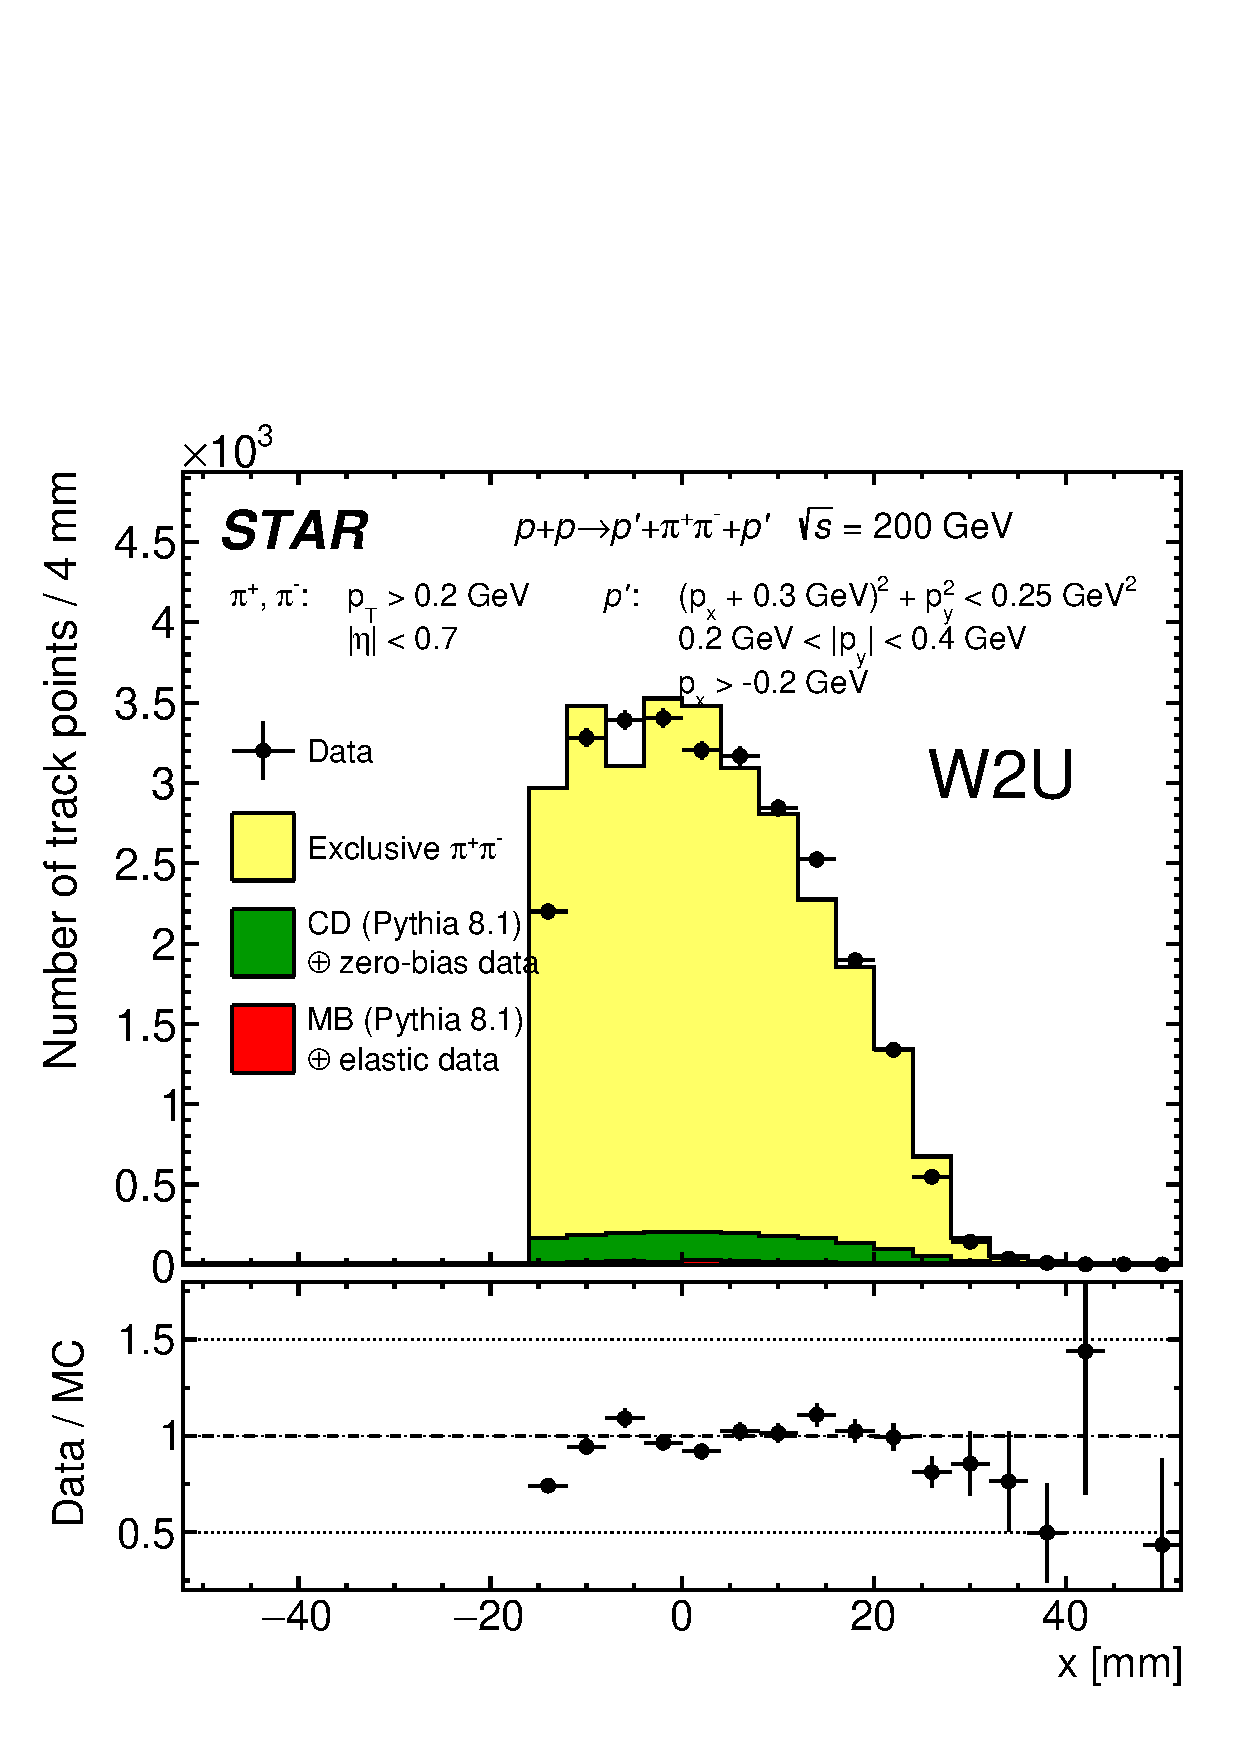
\includegraphics[width=\linewidth]{graphics/eventSelection/RpTracks/Ratio_Linear_x_W2U.pdf}\vspace*{-10pt}}
  \end{subfigure}\\[5pt]
  \begin{subfigure}[b]{\linewidth}%\addtocounter{subfigure}{1}
                \subcaptionbox{\label{fig:Ratio_Linear_x_W1D}}{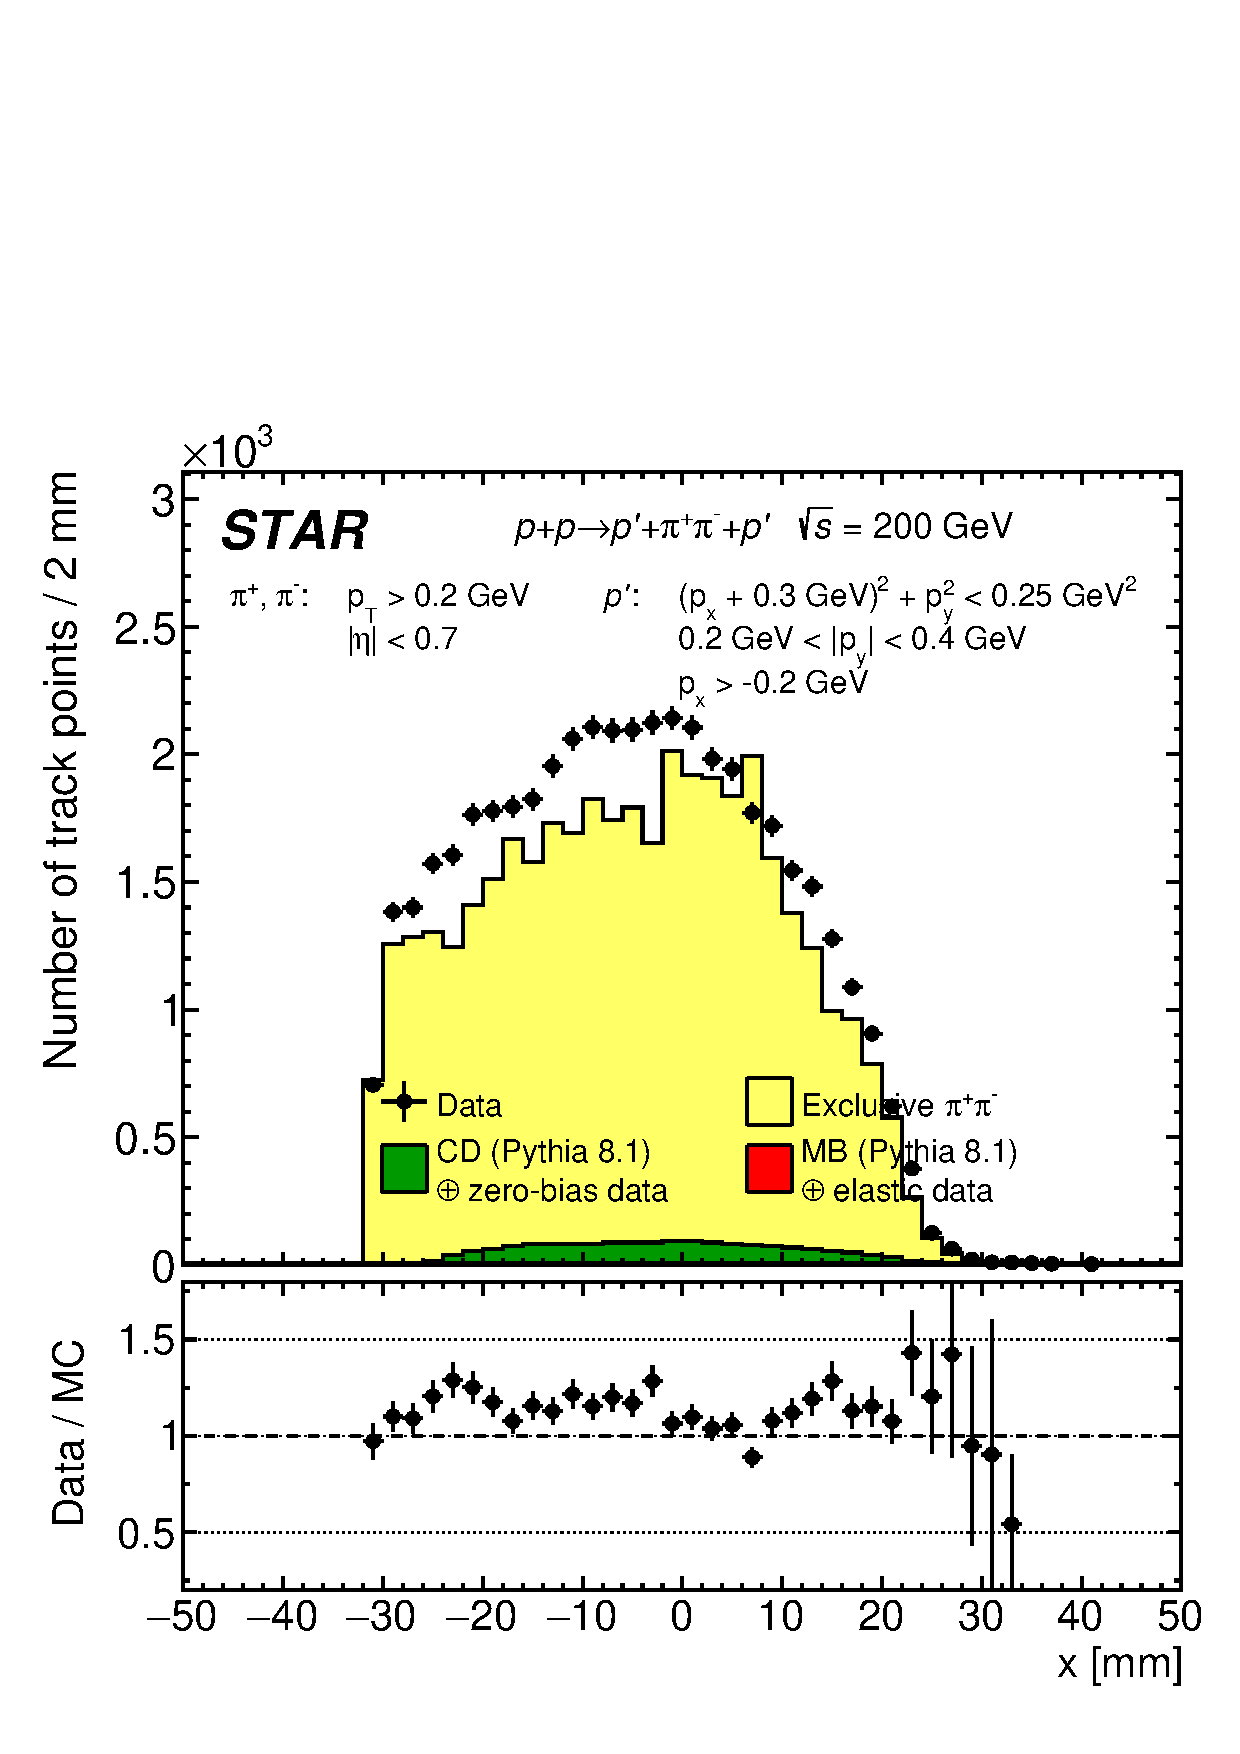
\includegraphics[width=\linewidth]{graphics/eventSelection/RpTracks/Ratio_Linear_x_W1D.pdf}\vspace*{-10pt}}
  \end{subfigure}
}%
\quad%
\parbox{0.31\textwidth}{
  \centering
  \begin{subfigure}[b]{\linewidth}%\addtocounter{subfigure}{-2}
                \subcaptionbox{\label{fig:Ratio_Linear_x_E2U}}{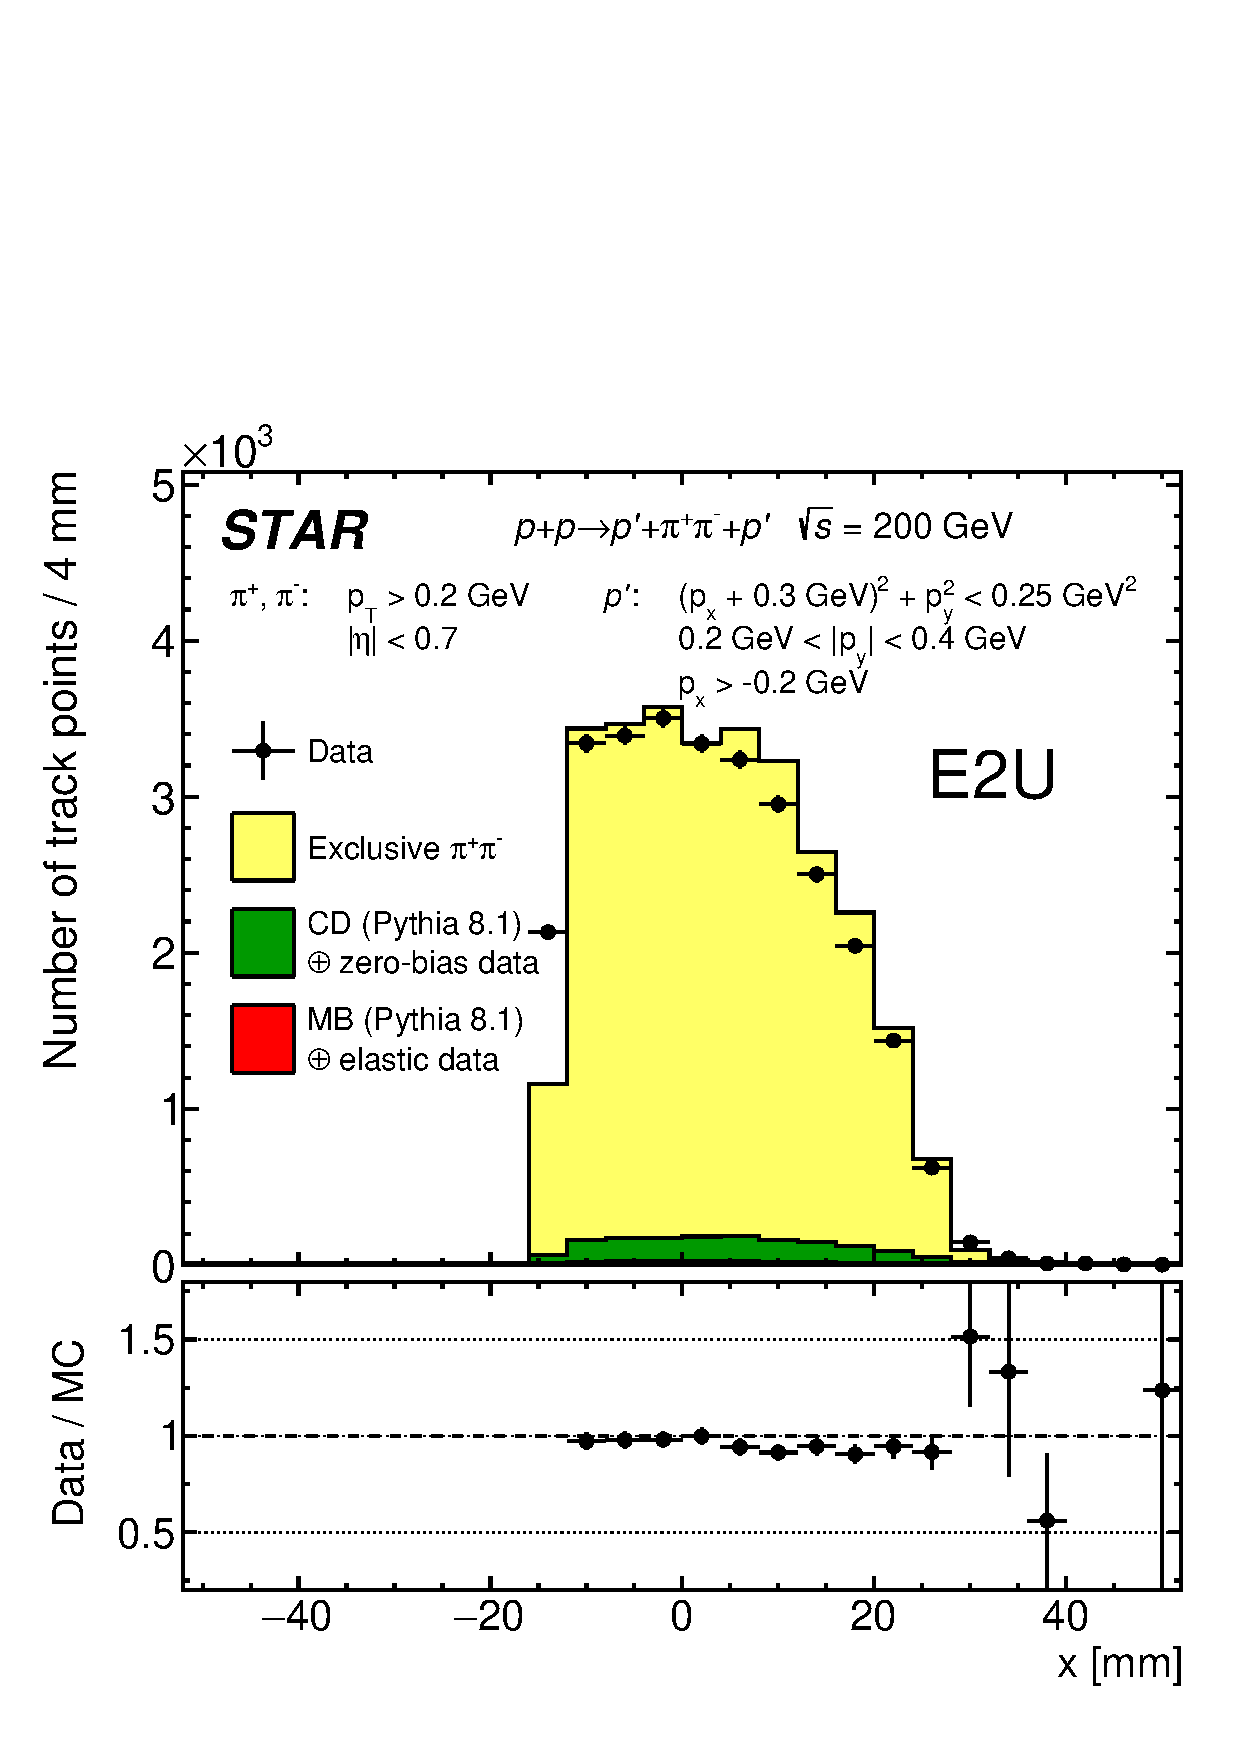
\includegraphics[width=\linewidth]{graphics/eventSelection/RpTracks/Ratio_Linear_x_E2U.pdf}\vspace*{-10pt}}
  \end{subfigure}\\[5pt]
  \begin{subfigure}[b]{\linewidth}%\addtocounter{subfigure}{1}
                \subcaptionbox{\label{fig:Ratio_Linear_x_E1D}}{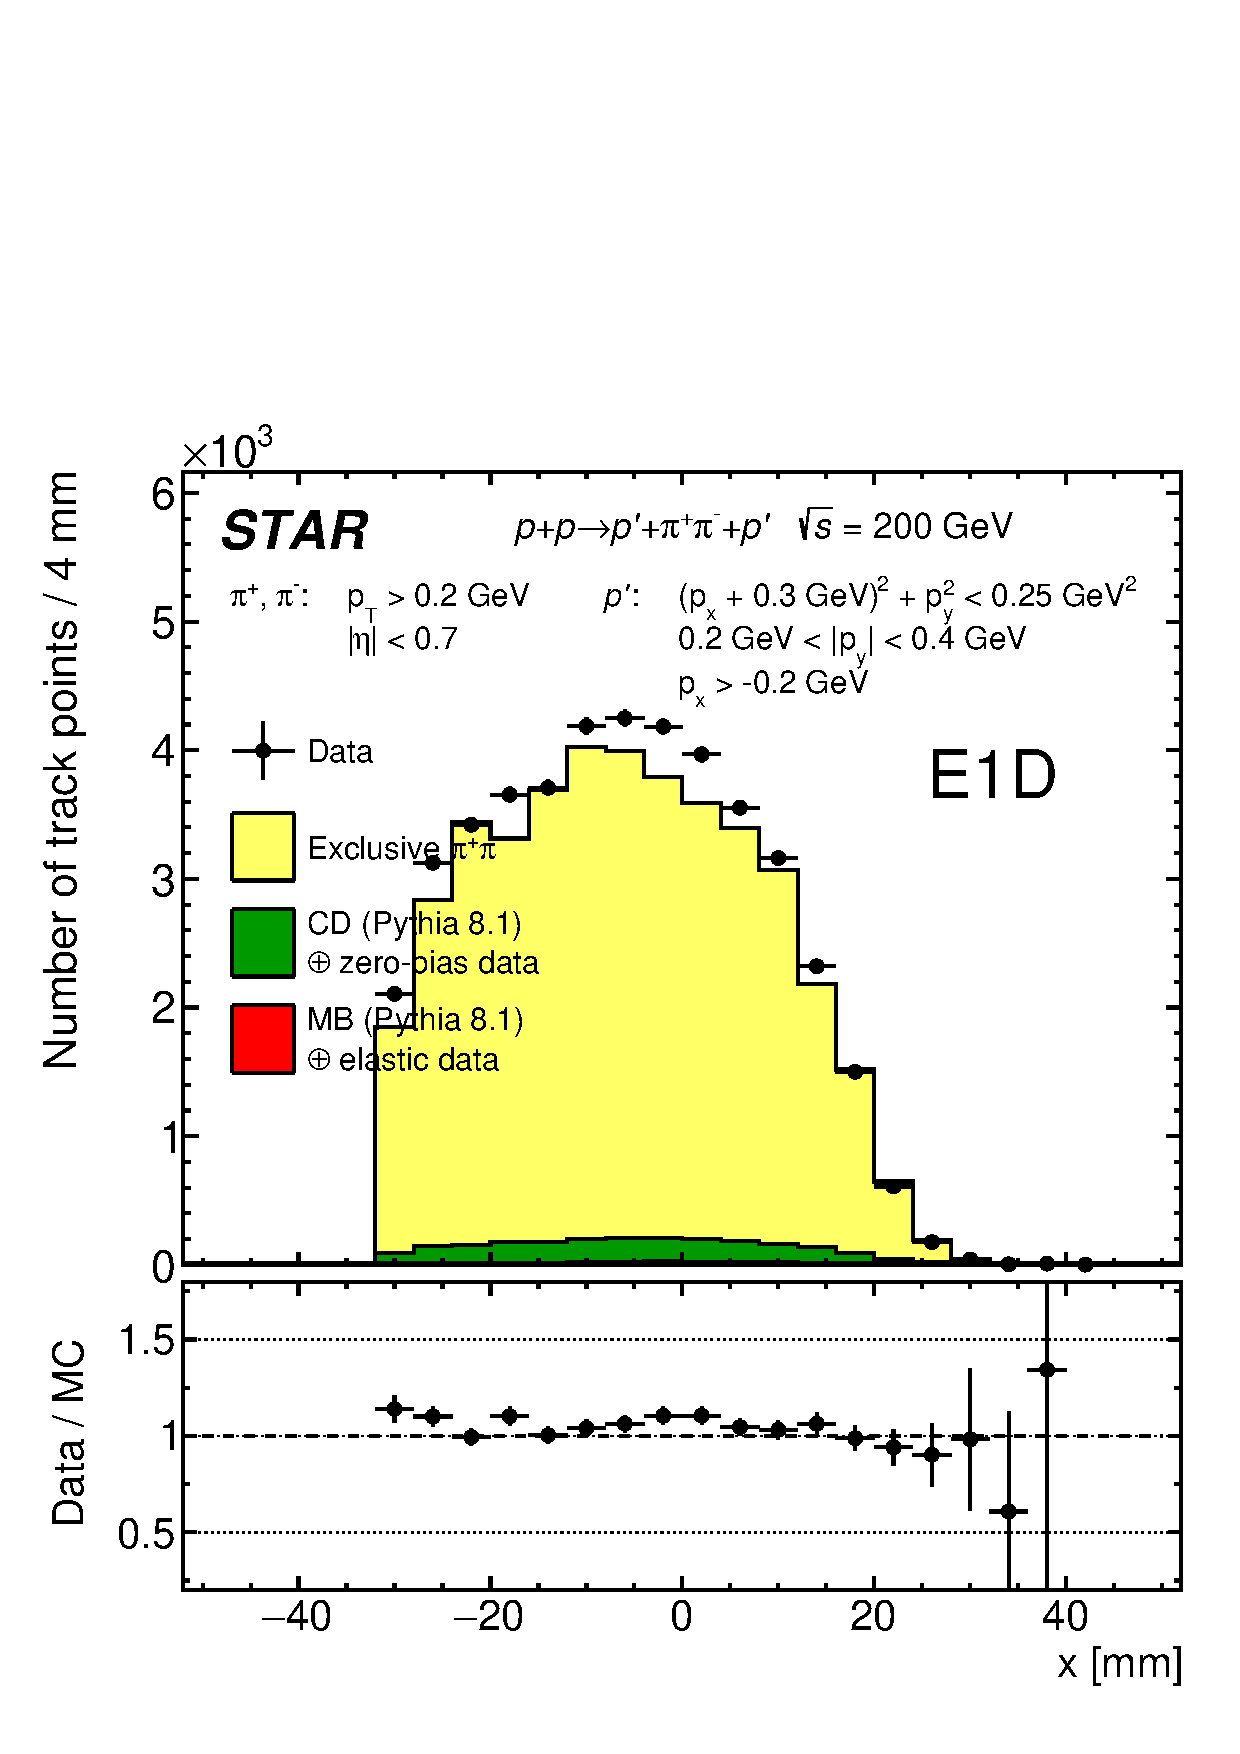
\includegraphics[width=\linewidth]{graphics/eventSelection/RpTracks/Ratio_Linear_x_E1D.pdf}\vspace*{-10pt}}
  \end{subfigure}\\[5pt]
  \begin{subfigure}[b]{\linewidth}%\addtocounter{subfigure}{1}
                \subcaptionbox{\label{fig:Ratio_Linear_x_W2D}}{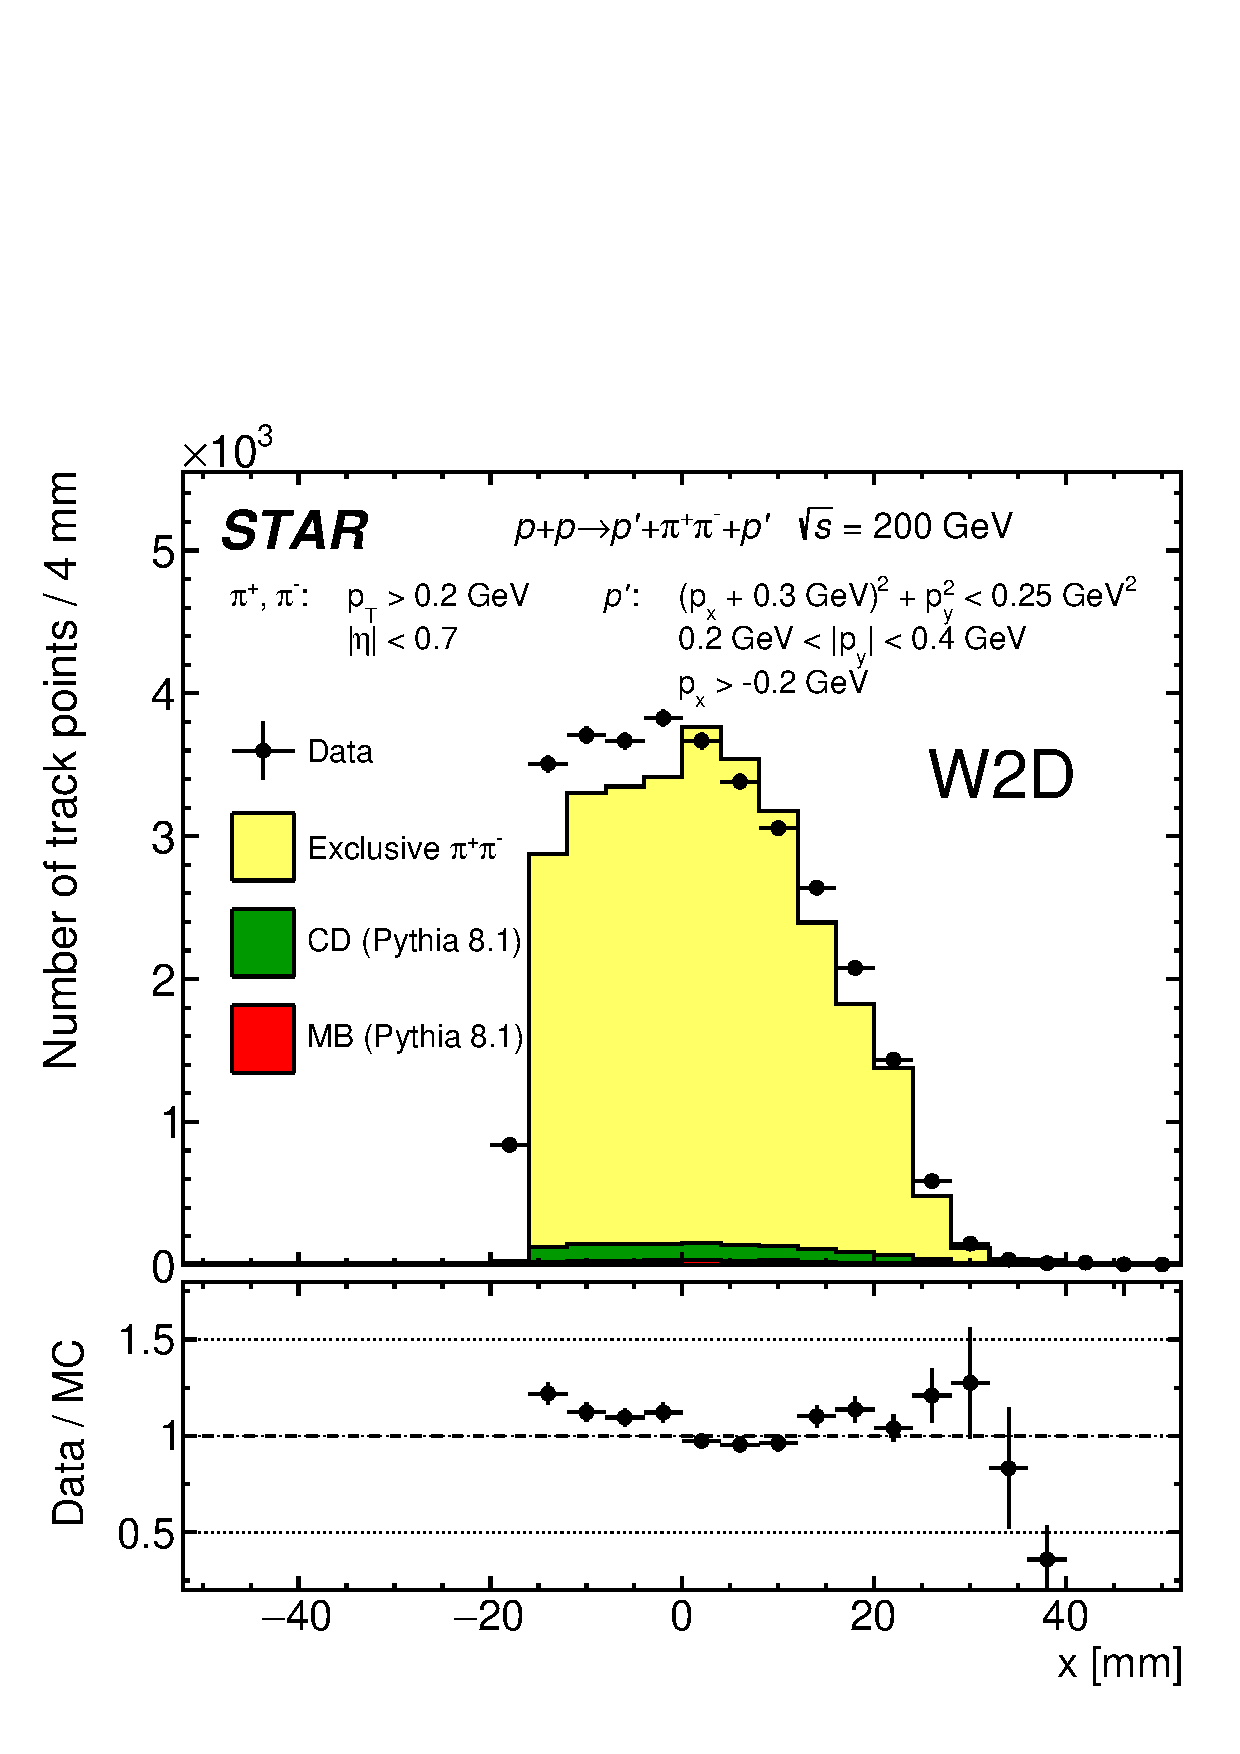
\includegraphics[width=\linewidth]{graphics/eventSelection/RpTracks/Ratio_Linear_x_W2D.pdf}\vspace*{-10pt}}
  \end{subfigure}
}%
\quad%
\parbox{0.31\textwidth}{
  \centering\vspace*{-22pt}
  \begin{subfigure}[b]{\linewidth}%\addtocounter{subfigure}{-2}
                \subcaptionbox{\label{fig:Ratio_Linear_x_W1U}}{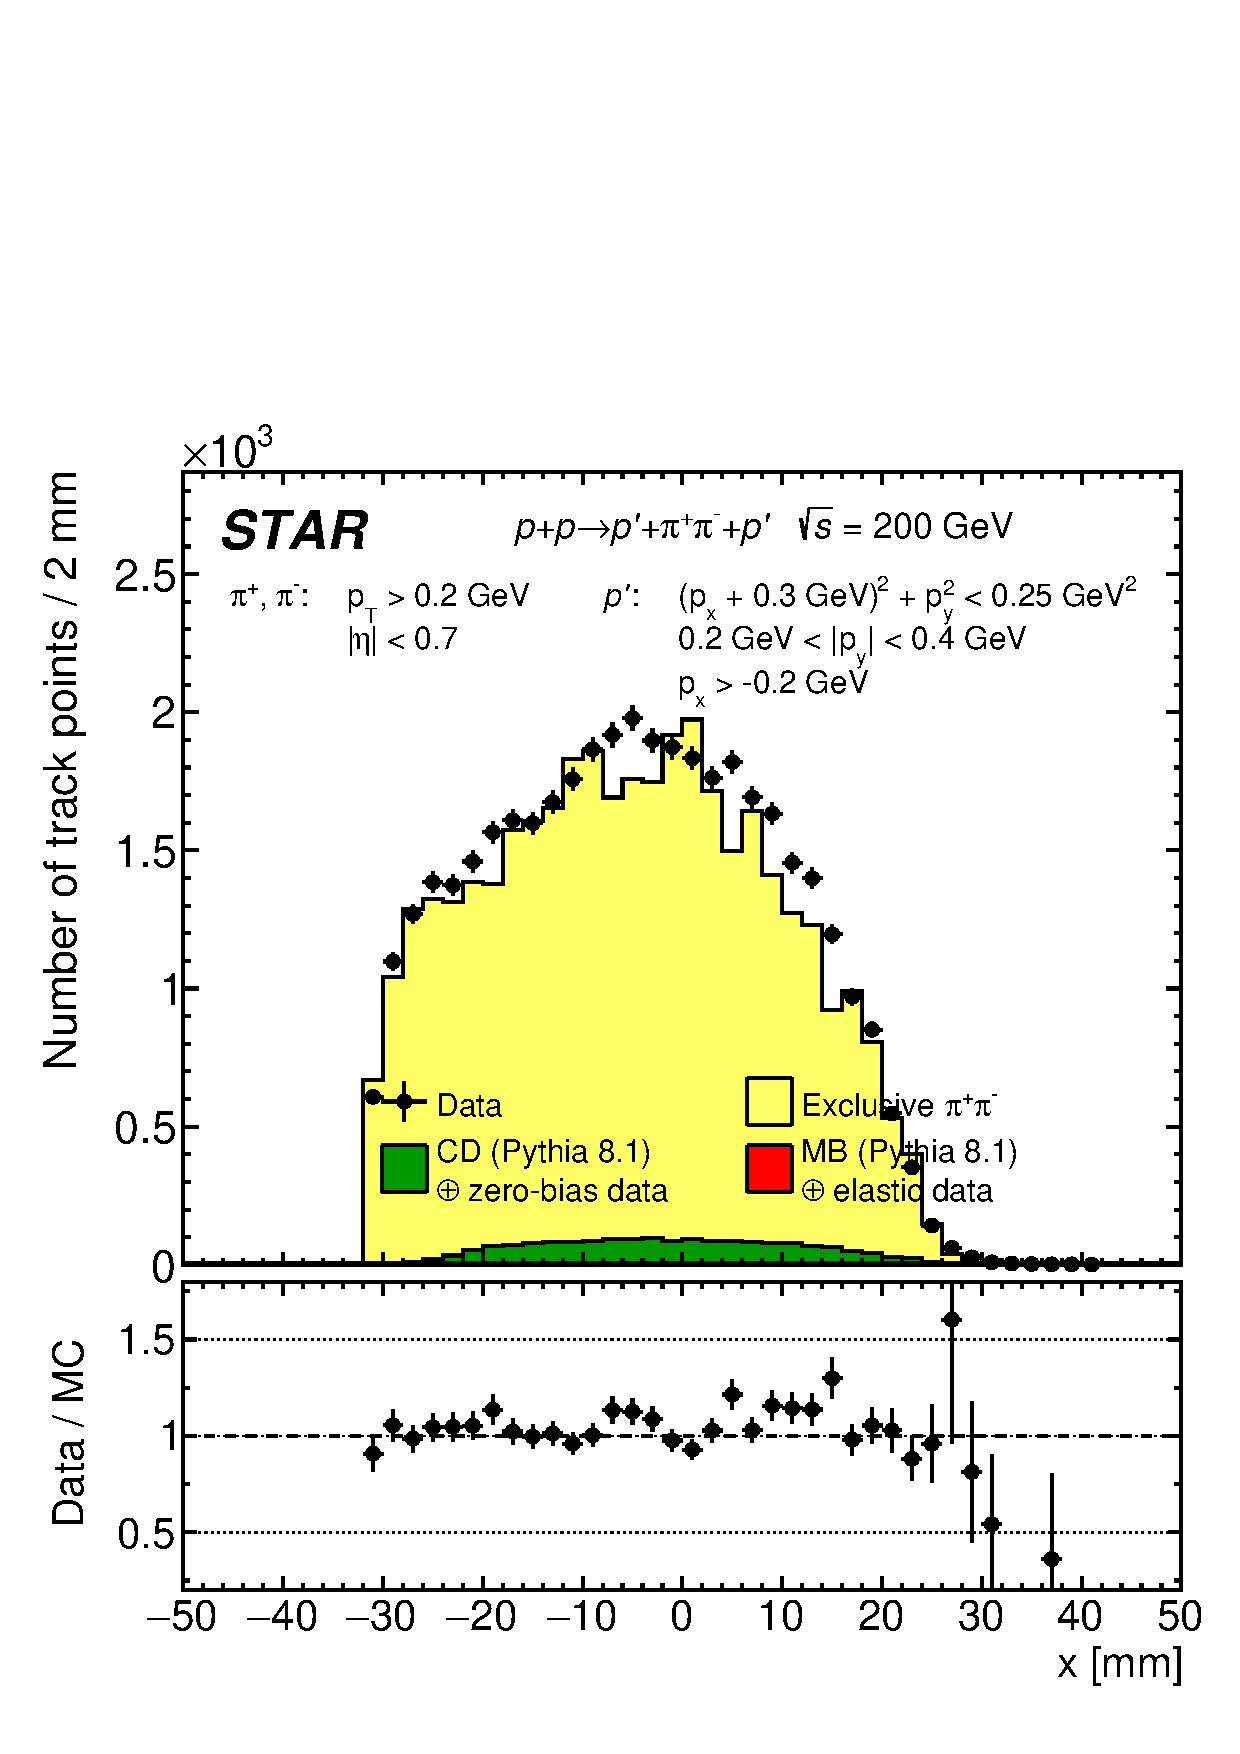
\includegraphics[width=\linewidth]{graphics/eventSelection/RpTracks/Ratio_Linear_x_W1U.pdf}\vspace*{-10pt}}
  \end{subfigure}\\[5pt]
  \begin{subfigure}[b]{\linewidth}%\addtocounter{subfigure}{1}
                \subcaptionbox{\label{fig:Ratio_Linear_x_E2D}}{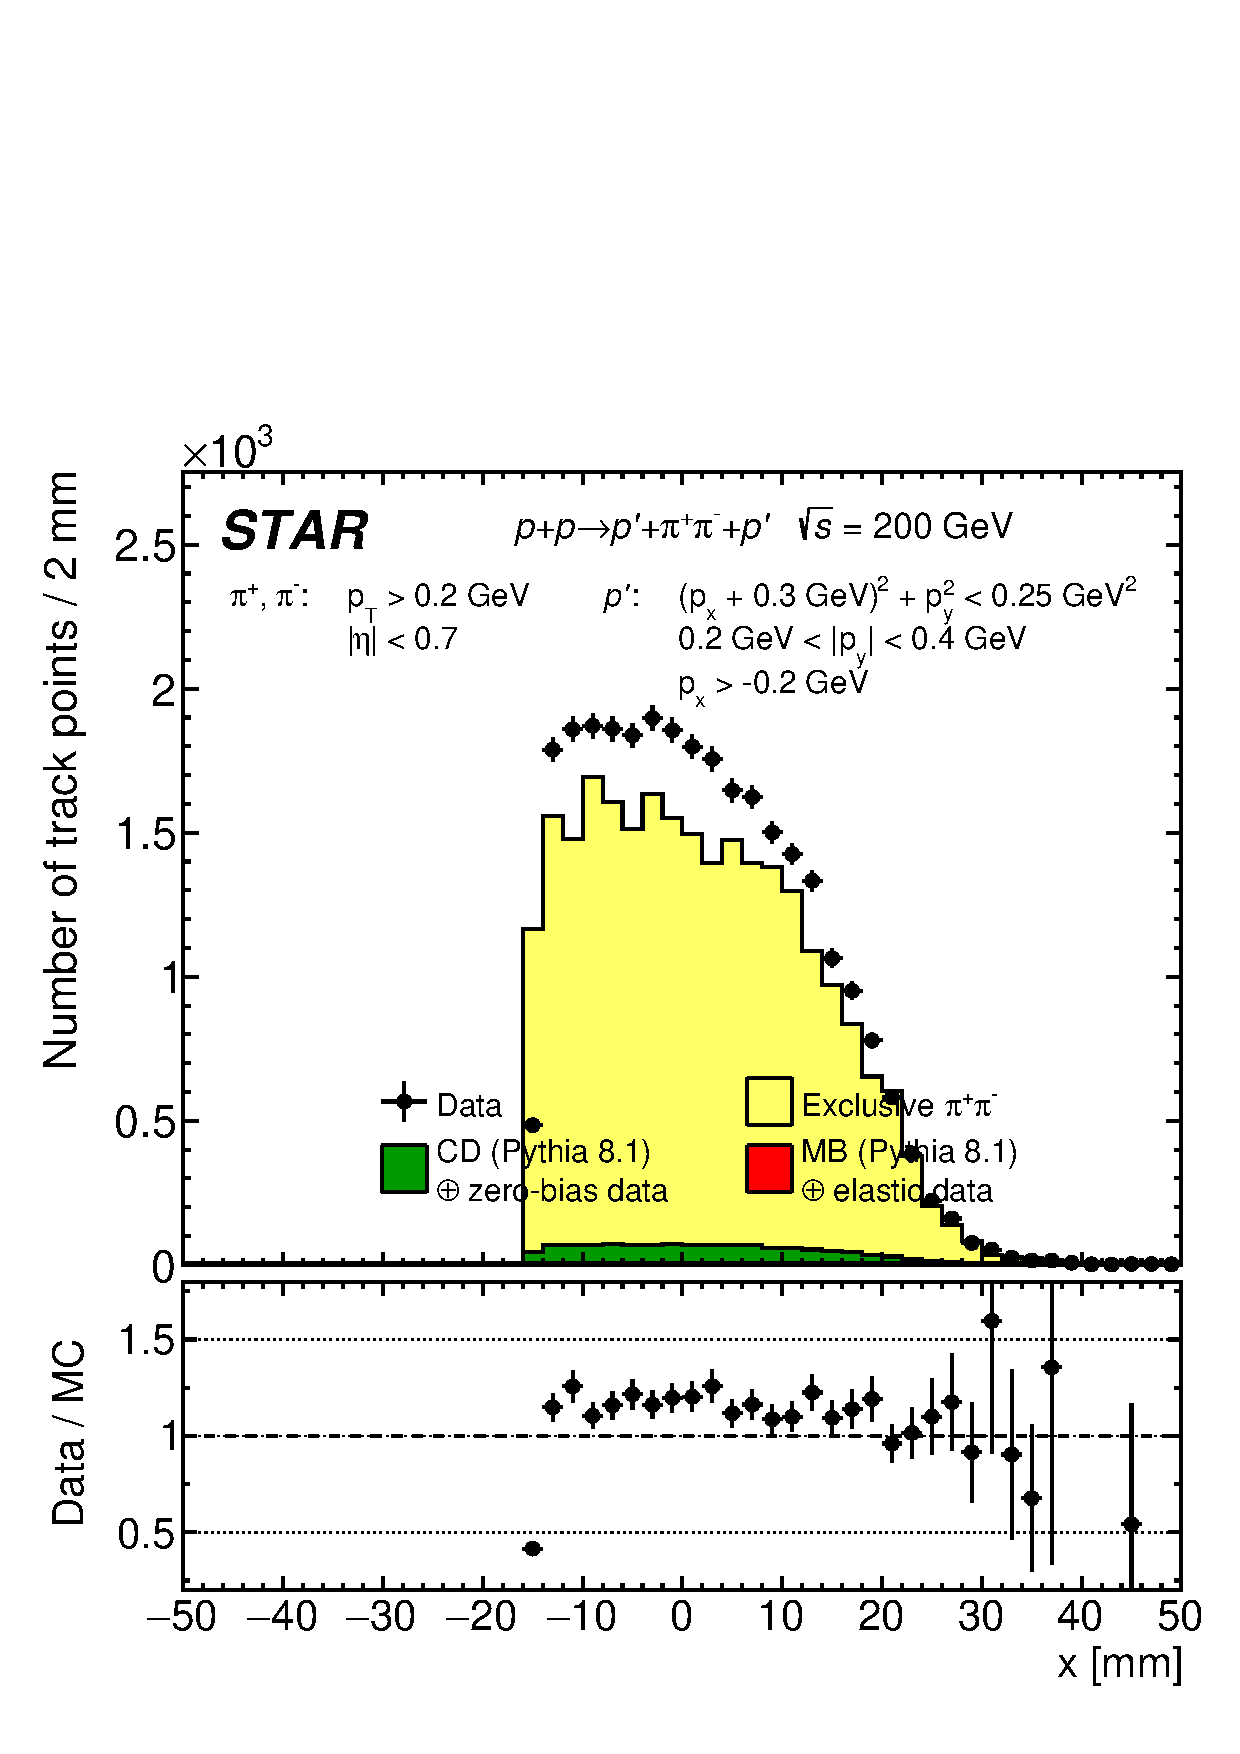
\includegraphics[width=\linewidth]{graphics/eventSelection/RpTracks/Ratio_Linear_x_E2D.pdf}\vspace*{-10pt}}
  \end{subfigure}
    \begin{minipage}[t][1.042\linewidth][t]{\linewidth}\end{minipage}
}
\caption[Comparison of $x$-position of track point between the data and stacked embedded MC.]{Comparison of $x$-position of track point between the data (black points) and stacked embedded MC (color histograms). Each subfigure corresponds to single RP station, whose name is printed in the right part subfigure. Vertical error bars represent statistical uncertainties, horizontal bars represent bin sizes. Normalizations of the signal and backgrounds were established according to description in Sec.~\ref{sec:bkgdSignalNorm}.}\label{fig:xRp}% 
\end{figure}
%---------------------------




%---------------------------
\begin{figure}[h]
\centering
\parbox{0.31\textwidth}{
  \centering
  \begin{subfigure}[b]{\linewidth}
                \subcaptionbox{\label{fig:Ratio_Linear_y_E1U}}{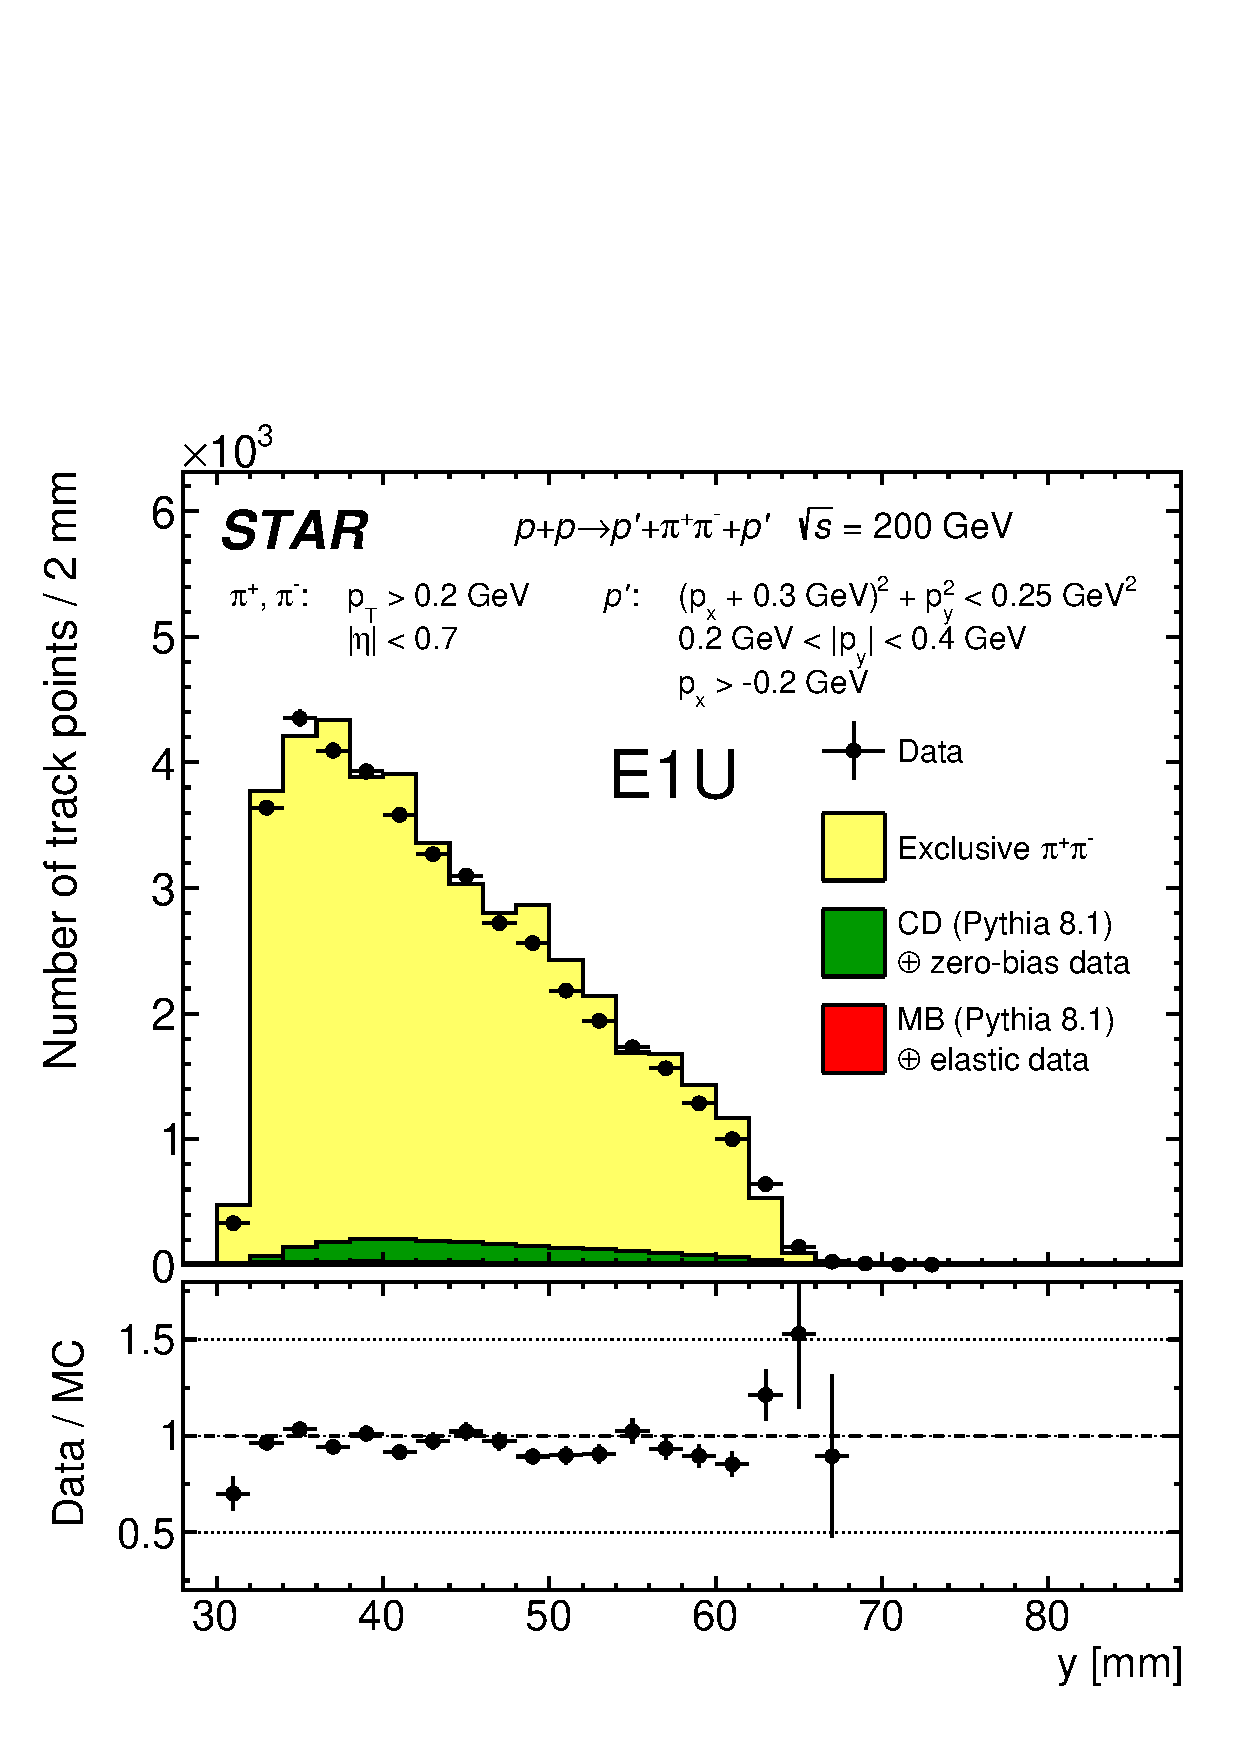
\includegraphics[width=\linewidth]{graphics/eventSelection/RpTracks/Ratio_Linear_y_E1U.pdf}\vspace*{-10pt}}
  \end{subfigure}\\[5pt]
  \begin{subfigure}[b]{\linewidth}%\addtocounter{subfigure}{1}
                \subcaptionbox{\label{fig:Ratio_Linear_y_W2U}}{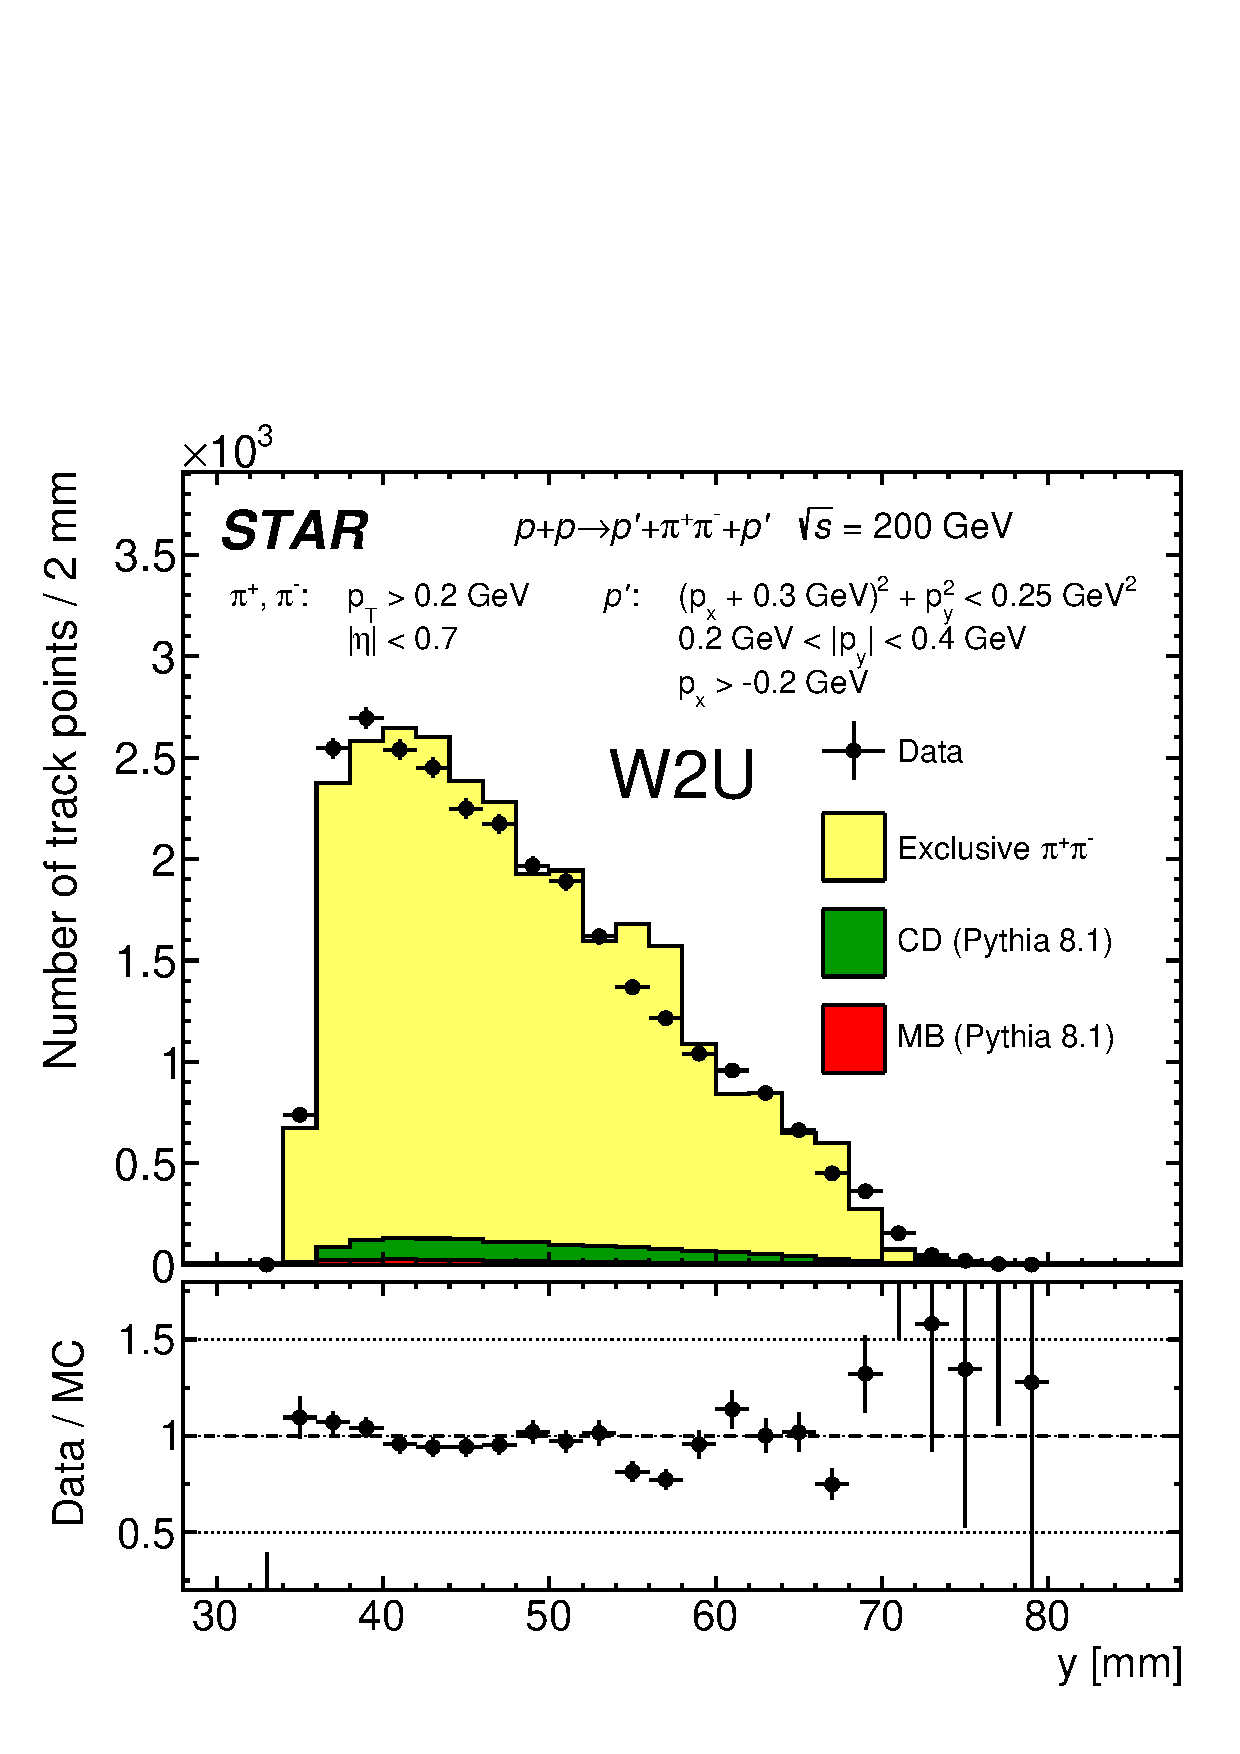
\includegraphics[width=\linewidth]{graphics/eventSelection/RpTracks/Ratio_Linear_y_W2U.pdf}\vspace*{-10pt}}
  \end{subfigure}\\[5pt]
  \begin{subfigure}[b]{\linewidth}%\addtocounter{subfigure}{1}
                \subcaptionbox{\label{fig:Ratio_Linear_y_W1D}}{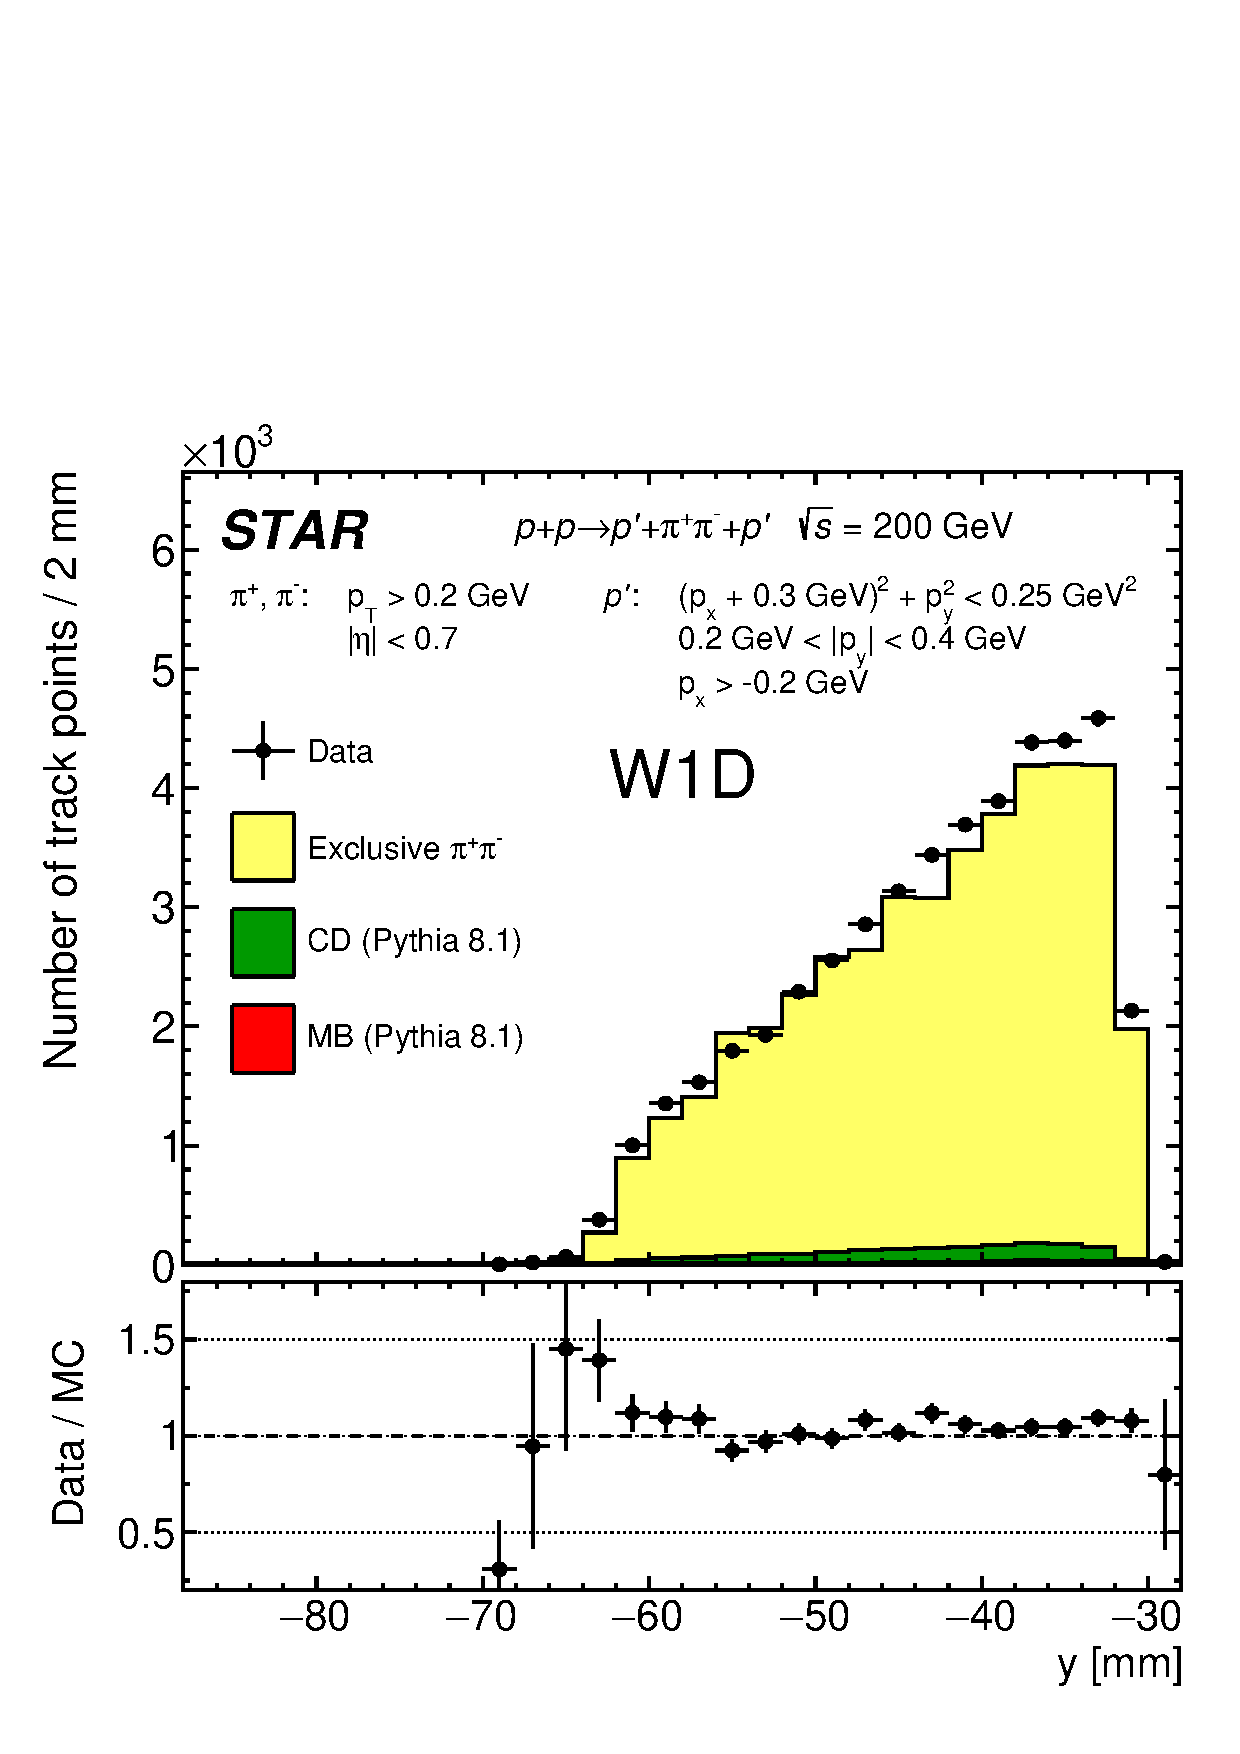
\includegraphics[width=\linewidth]{graphics/eventSelection/RpTracks/Ratio_Linear_y_W1D.pdf}\vspace*{-10pt}}
  \end{subfigure}
}%
\quad%
\parbox{0.31\textwidth}{
  \centering
  \begin{subfigure}[b]{\linewidth}%\addtocounter{subfigure}{-2}
                \subcaptionbox{\label{fig:Ratio_Linear_y_E2U}}{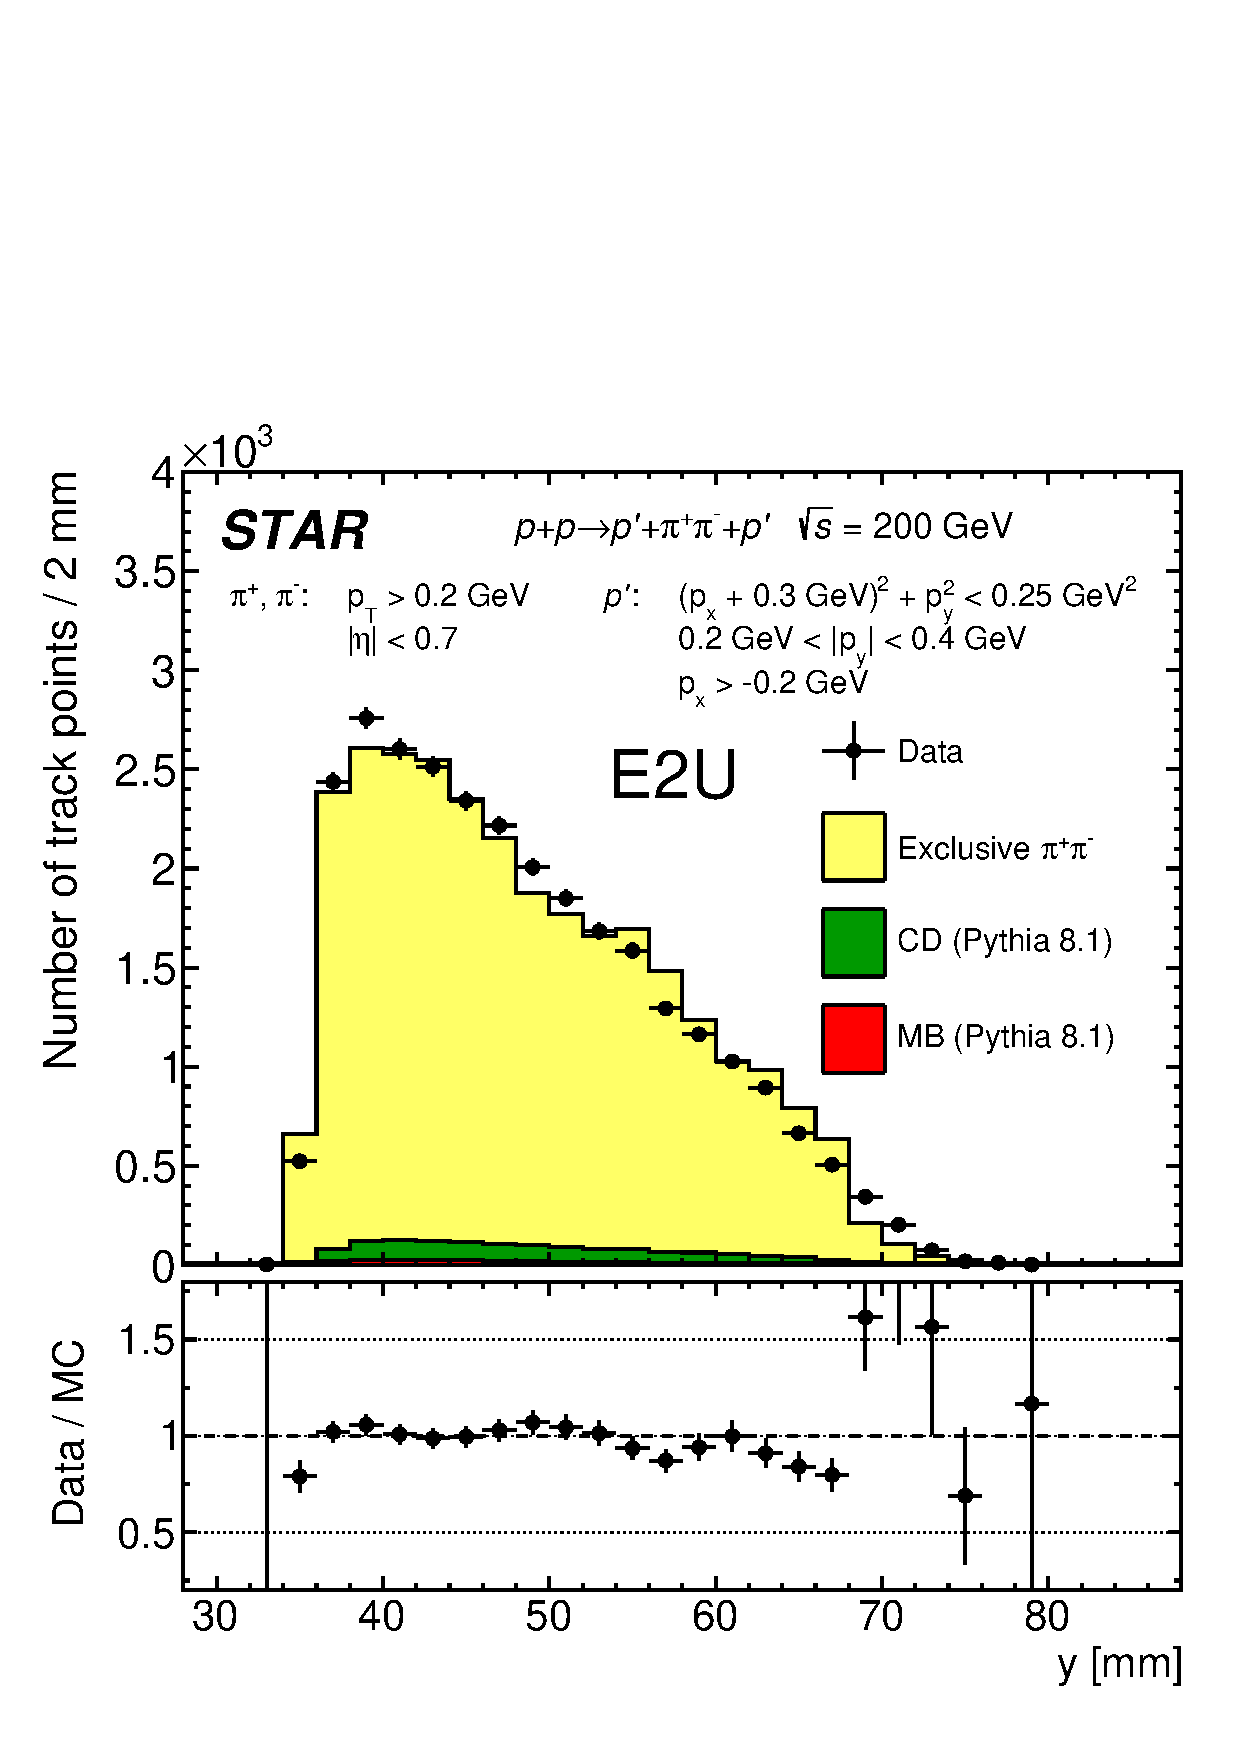
\includegraphics[width=\linewidth]{graphics/eventSelection/RpTracks/Ratio_Linear_y_E2U.pdf}\vspace*{-10pt}}
  \end{subfigure}\\[5pt]
  \begin{subfigure}[b]{\linewidth}%\addtocounter{subfigure}{1}
                \subcaptionbox{\label{fig:Ratio_Linear_y_E1D}}{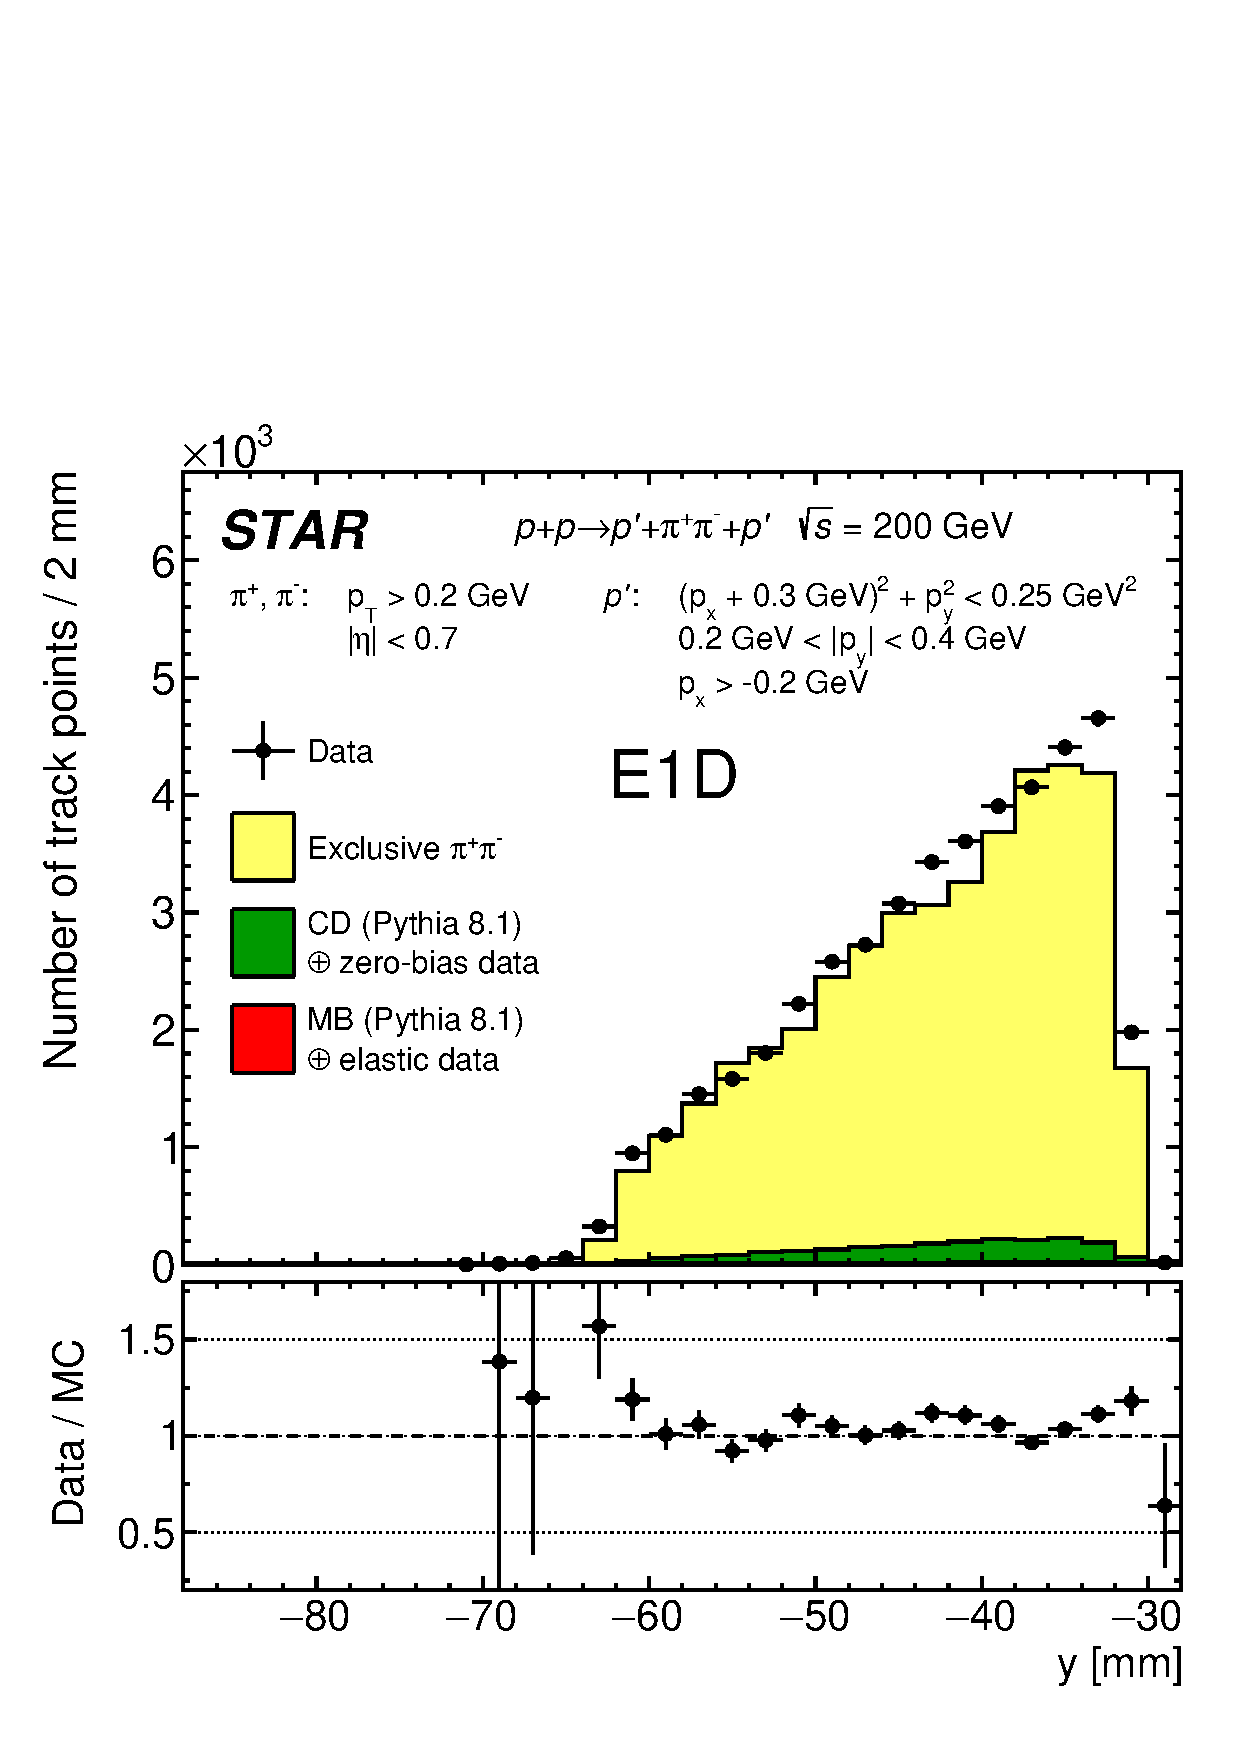
\includegraphics[width=\linewidth]{graphics/eventSelection/RpTracks/Ratio_Linear_y_E1D.pdf}\vspace*{-10pt}}
  \end{subfigure}\\
  \begin{subfigure}[b]{\linewidth}%\addtocounter{subfigure}{1}
                \subcaptionbox{\label{fig:Ratio_Linear_y_W2D}}{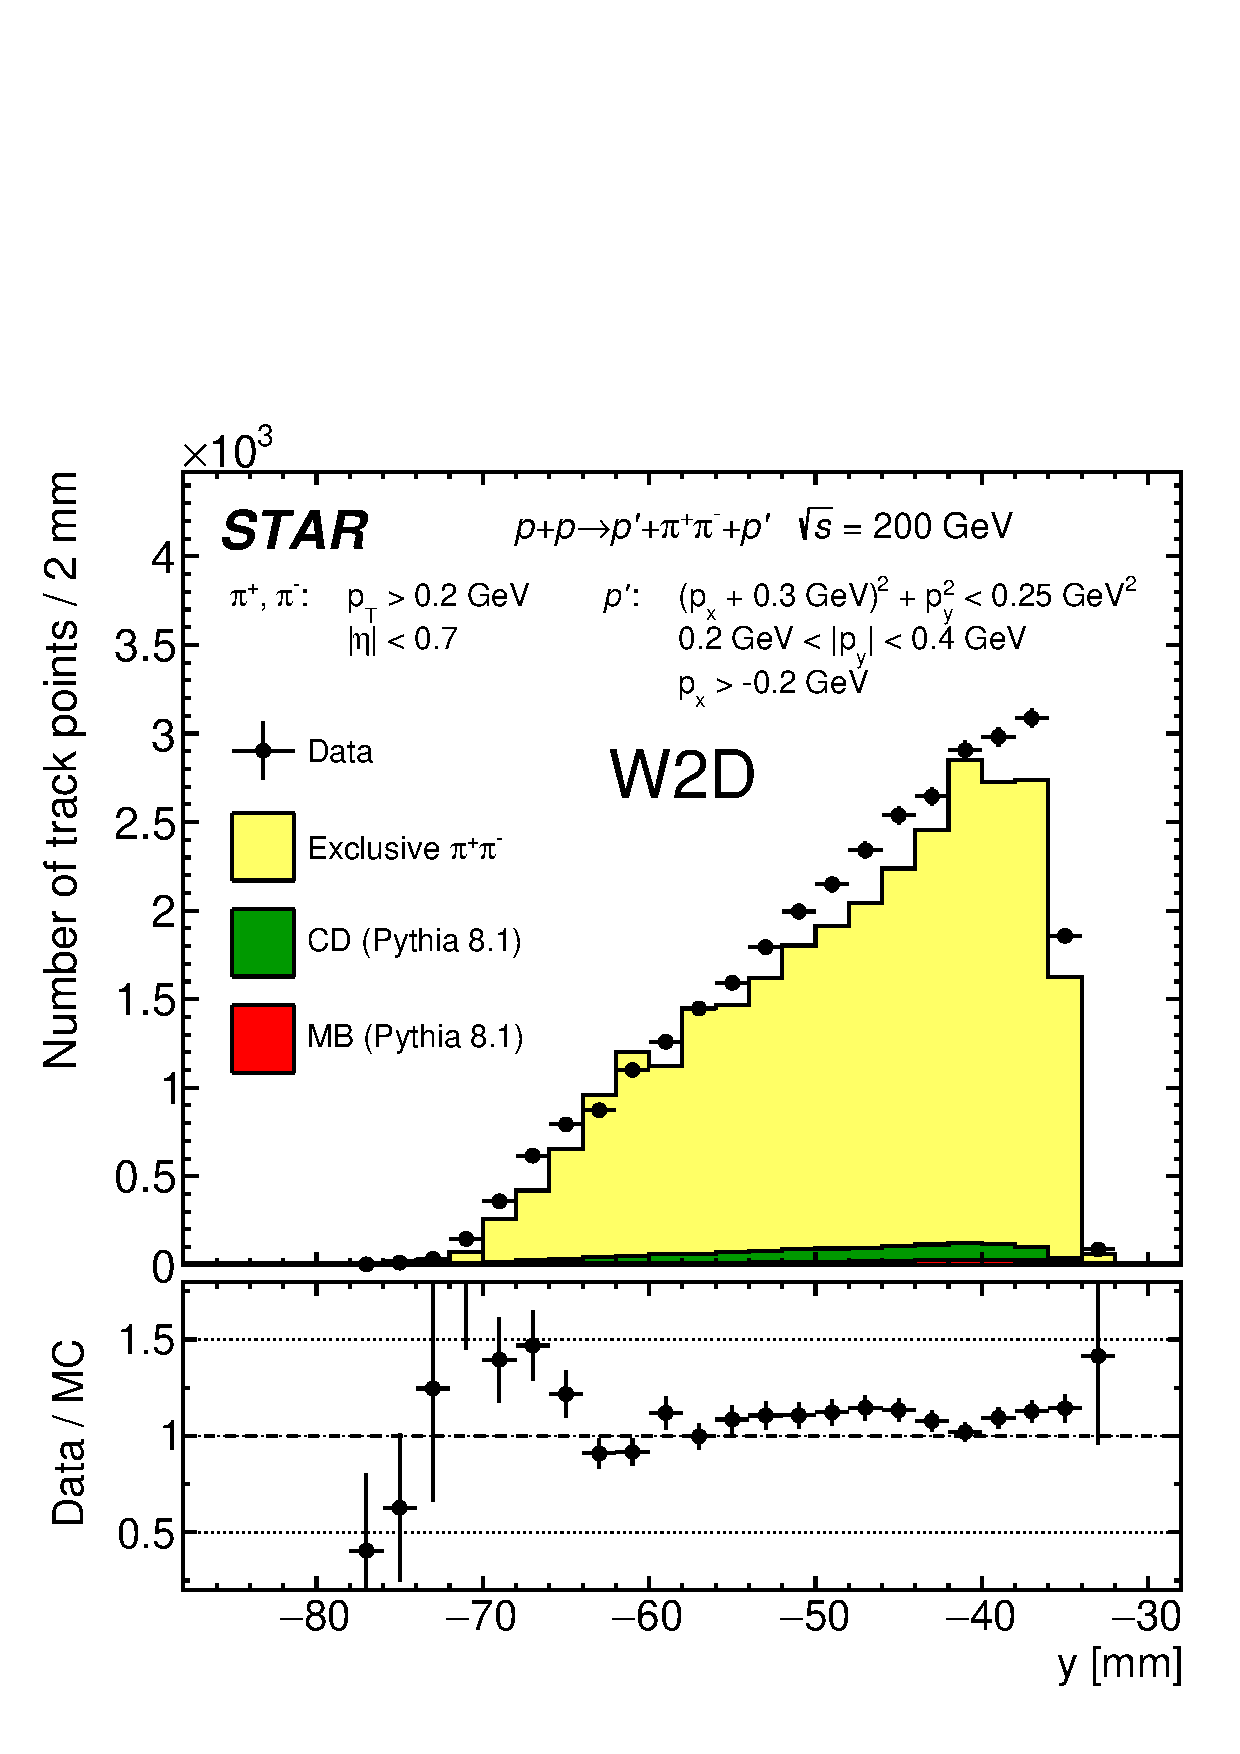
\includegraphics[width=\linewidth]{graphics/eventSelection/RpTracks/Ratio_Linear_y_W2D.pdf}\vspace*{-10pt}}
  \end{subfigure}
}%
\quad%
\parbox{0.31\textwidth}{
  \centering\vspace*{-22pt}
  \begin{subfigure}[b]{\linewidth}%\addtocounter{subfigure}{-2}
                \subcaptionbox{\label{fig:Ratio_Linear_y_W1U}}{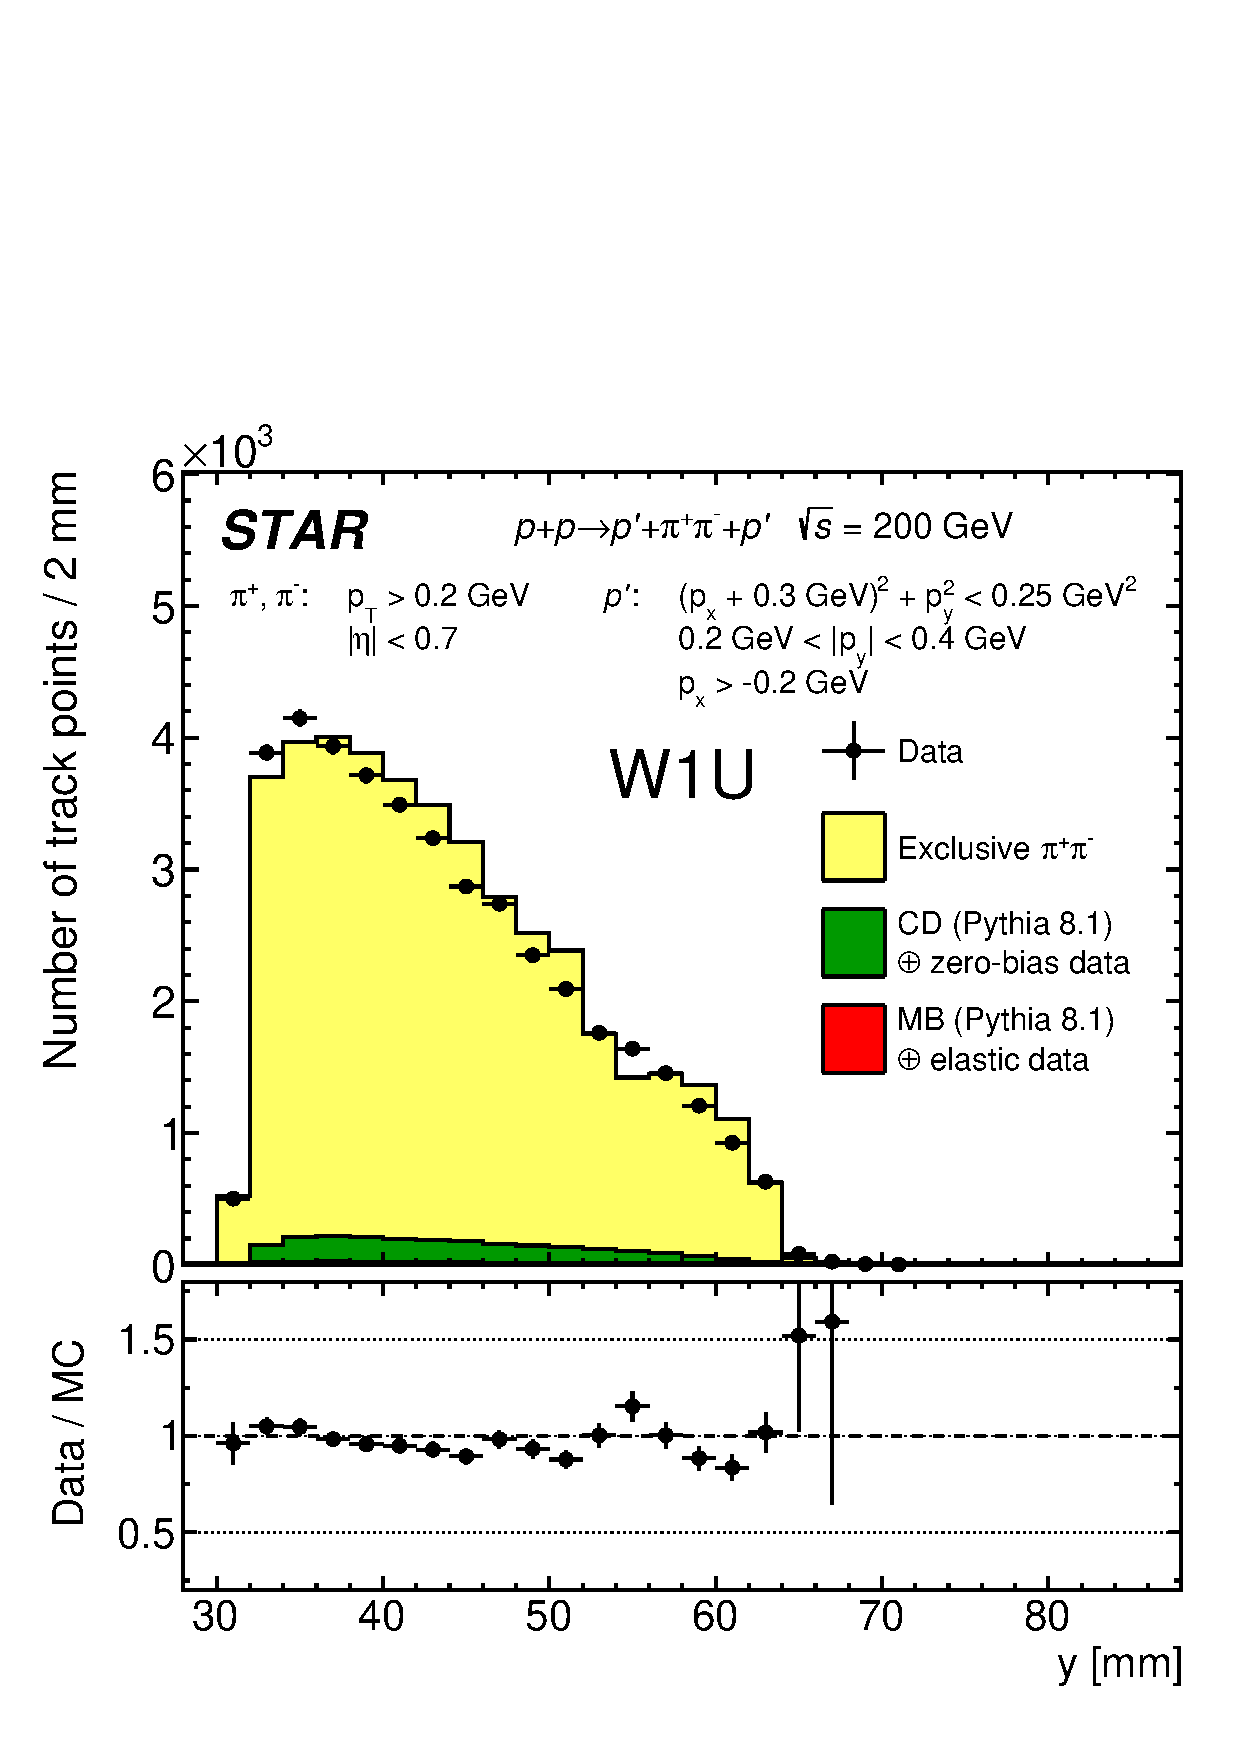
\includegraphics[width=\linewidth]{graphics/eventSelection/RpTracks/Ratio_Linear_y_W1U.pdf}\vspace*{-10pt}}
  \end{subfigure}\\[5pt]
  \begin{subfigure}[b]{\linewidth}%\addtocounter{subfigure}{1}
                \subcaptionbox{\label{fig:Ratio_Linear_y_E2D}}{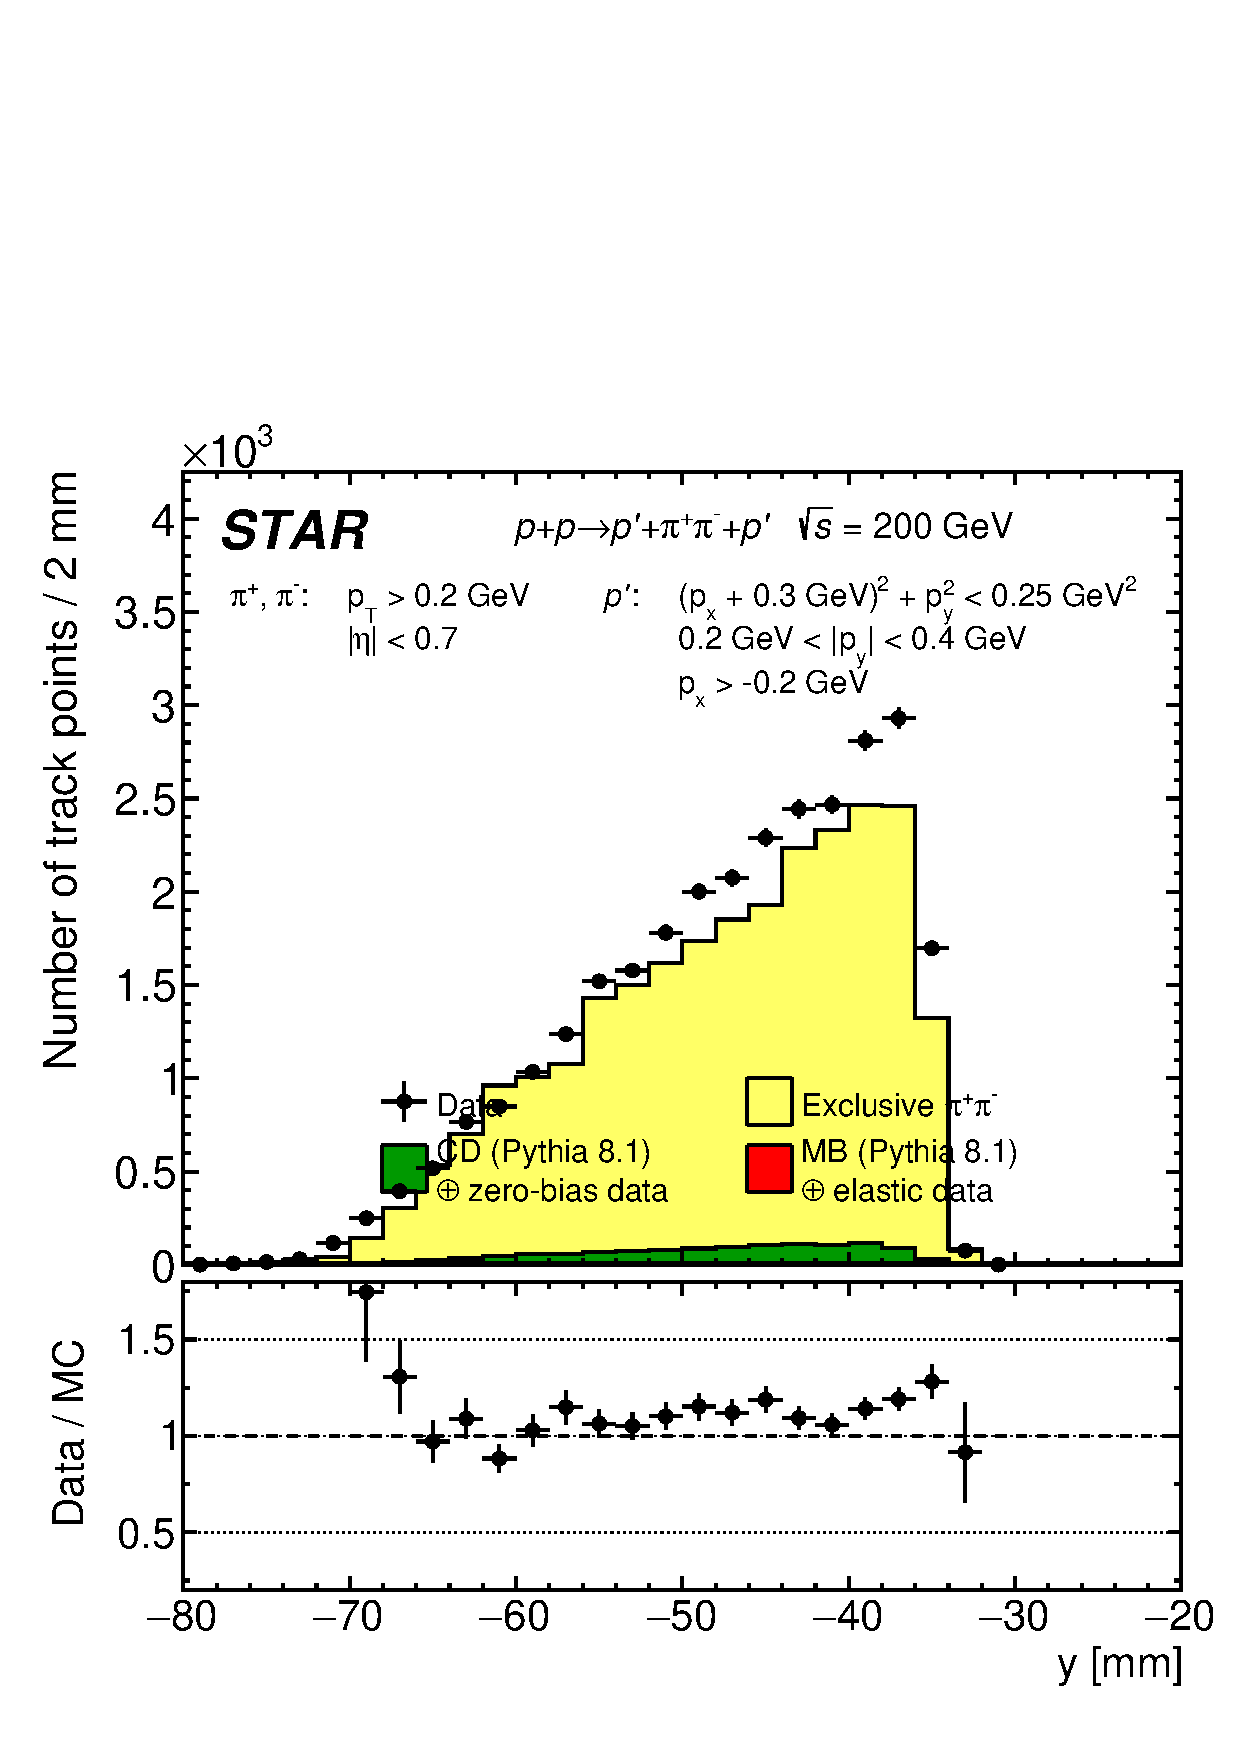
\includegraphics[width=\linewidth]{graphics/eventSelection/RpTracks/Ratio_Linear_y_E2D.pdf}\vspace*{-10pt}}
  \end{subfigure}
    \begin{minipage}[t][1.042\linewidth][t]{\linewidth}\end{minipage}
}
\caption[Comparison of $y$-position of track point between the data and stacked embedded MC.]{Comparison of $y$-position of track point between the data (black points) and stacked embedded MC (color histograms). Each subfigure corresponds to single RP station, whose name is printed in the middle of subfigure. Vertical error bars represent statistical uncertainties, horizontal bars represent bin sizes. Normalizations of the signal and backgrounds were established according to description in Sec.~\ref{sec:bkgdSignalNorm}.}\label{fig:yRp}% 
\end{figure}
%---------------------------






%%%%%%%%%%%%%%%%%%%%%%%%%%%%%%%%%%%%%%%%%%%%%%%%%%%%%%%%%%%%%%%%%%%%%%%%%%%%%%%%%%%%%%%%%%%%%%%%%%%%%%%%%%%%%%%%%%%%%%%%%%%%%%%%%%%%
\subsection{(\ref{enum:CutDeltaZVx})~TPC-RP \texorpdfstring{$z$}{z}-vertex matching}\label{sec:C5}

In CEP tracks in the central detector and tracks in Roman Pots originate from the same interaction vertex. Measurement of the time of detection of forward protons in RPs gives access to reconstruction of the position of the vertex
\begin{equation}
z_{\text{vtx}}^{\text{RP}} = c\cdot\frac{t^{\text{RP}}_{\text{W}} - t^{\text{RP}}_{\text{E}}}{2}
\end{equation}
independently from TPC, which allows their comparison and rejection of the background if the two values disagree. Time of detection of proton in RP is provided in StMuRpsTrack object - it is an average of all TAC values from PMTs in RPs used to form a track, corrected for the slewing effect and adjusted to have the best correlation with the $z$-position of the vertex measured in TPC, translated to unit of time (all these steps are done at the level of raw data reconstruction). In Fig.~\ref{fig:zVertexRpTpc} the comparisons of the $z_{\text{vtx}}^{\text{RP}}$ and $z_{\text{vtx}}^{\text{TPC}}$ are shown with some preselection cuts applied. A clear signal from the Central Diffraction (and thus CEP) process is manifesting in high correlation of the two values (diagonal in Fig.~\ref{fig:zVertexRpVsTpc}) or significant and relatively narrow peak centered at 0 for the difference of two values (Fig.~\ref{fig:zVertexRpMinusZVertexTpc}). %
%---------------------------
\begin{figure}[ht!]
\centering
\parbox{0.4\textwidth}{
  \centering
  \begin{subfigure}[b]{\linewidth}{
                \subcaptionbox{\label{fig:zVertexRpVsTpc}}{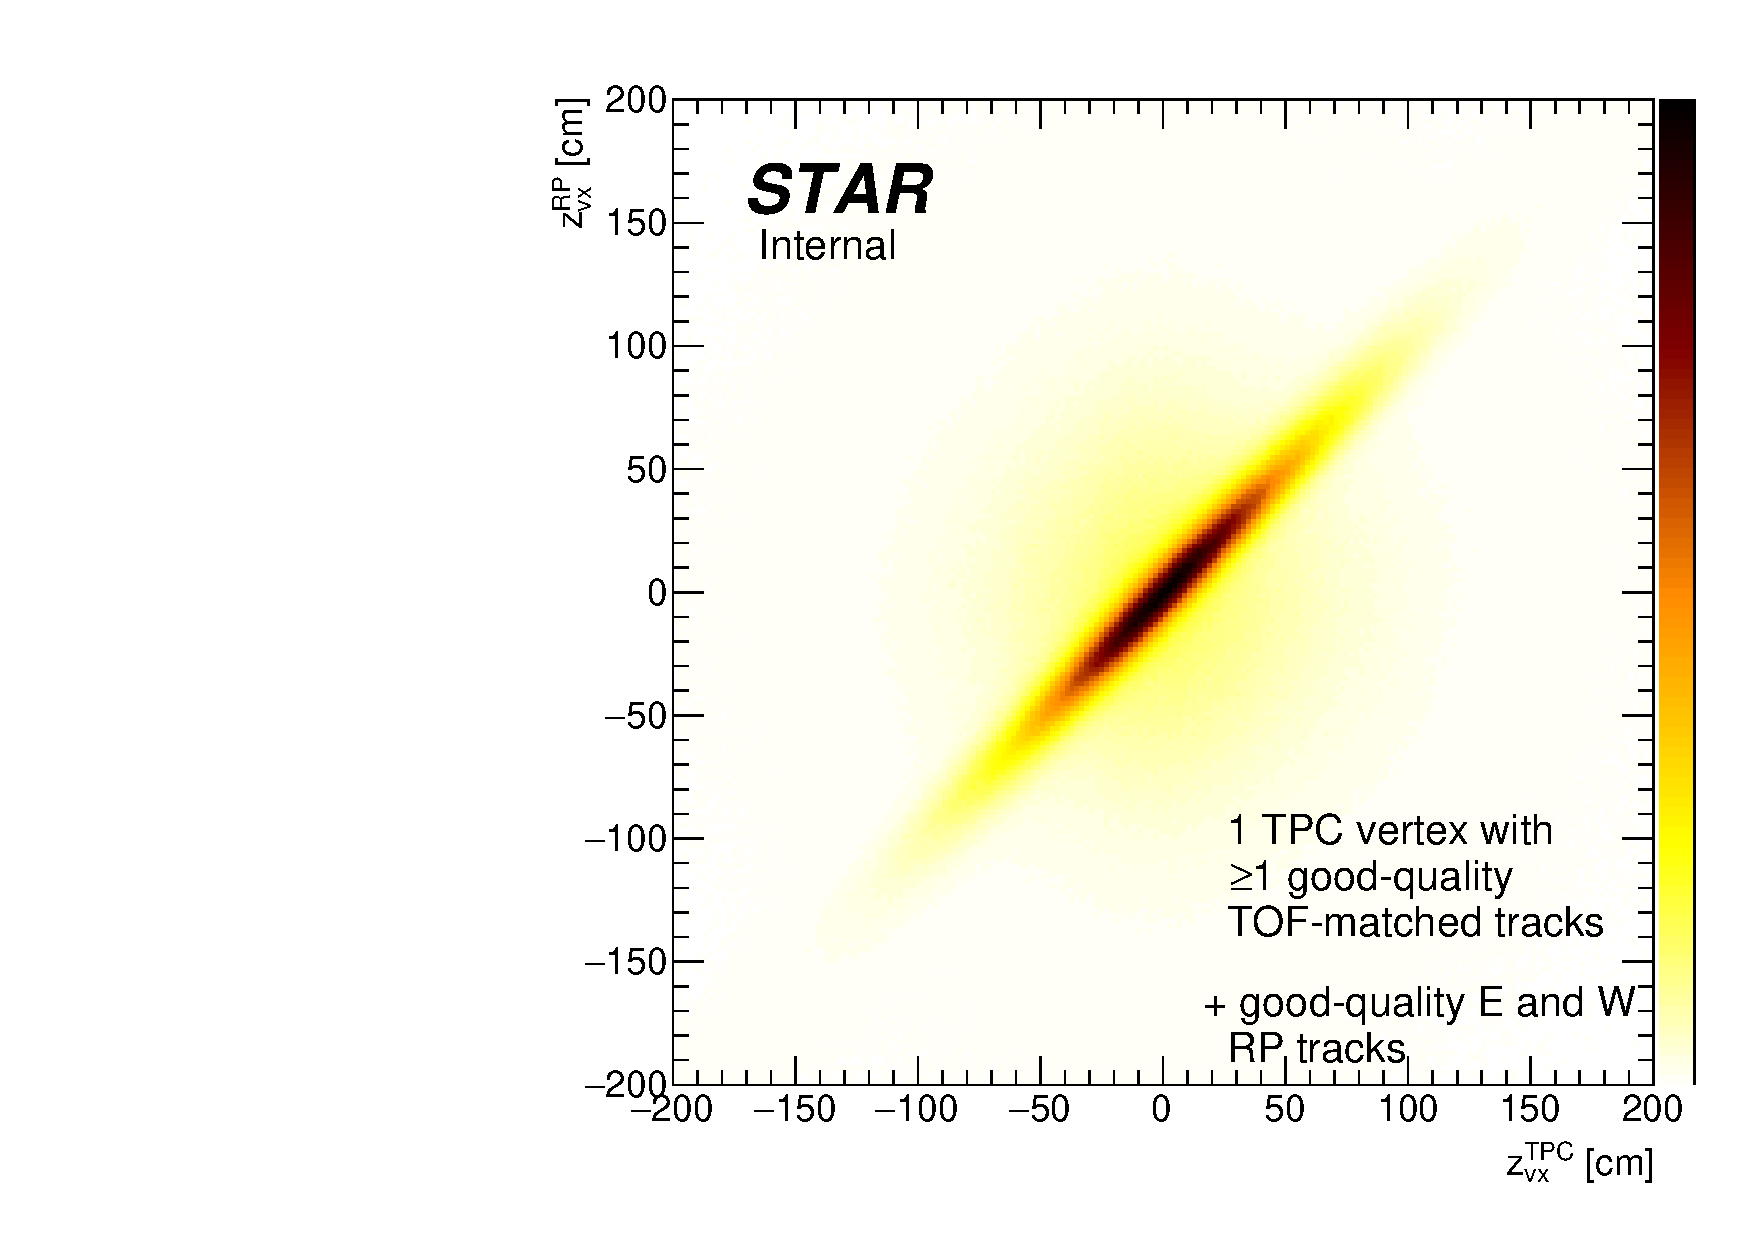
\includegraphics[width=\linewidth]{graphics/eventSelection/zVertexRpVsTpc.pdf}}}
  \end{subfigure}
}
\quad
\parbox{0.545\textwidth}{
  \centering
  \begin{subfigure}[b]{\linewidth}{
                \subcaptionbox{\label{fig:zVertexRpMinusZVertexTpc}}{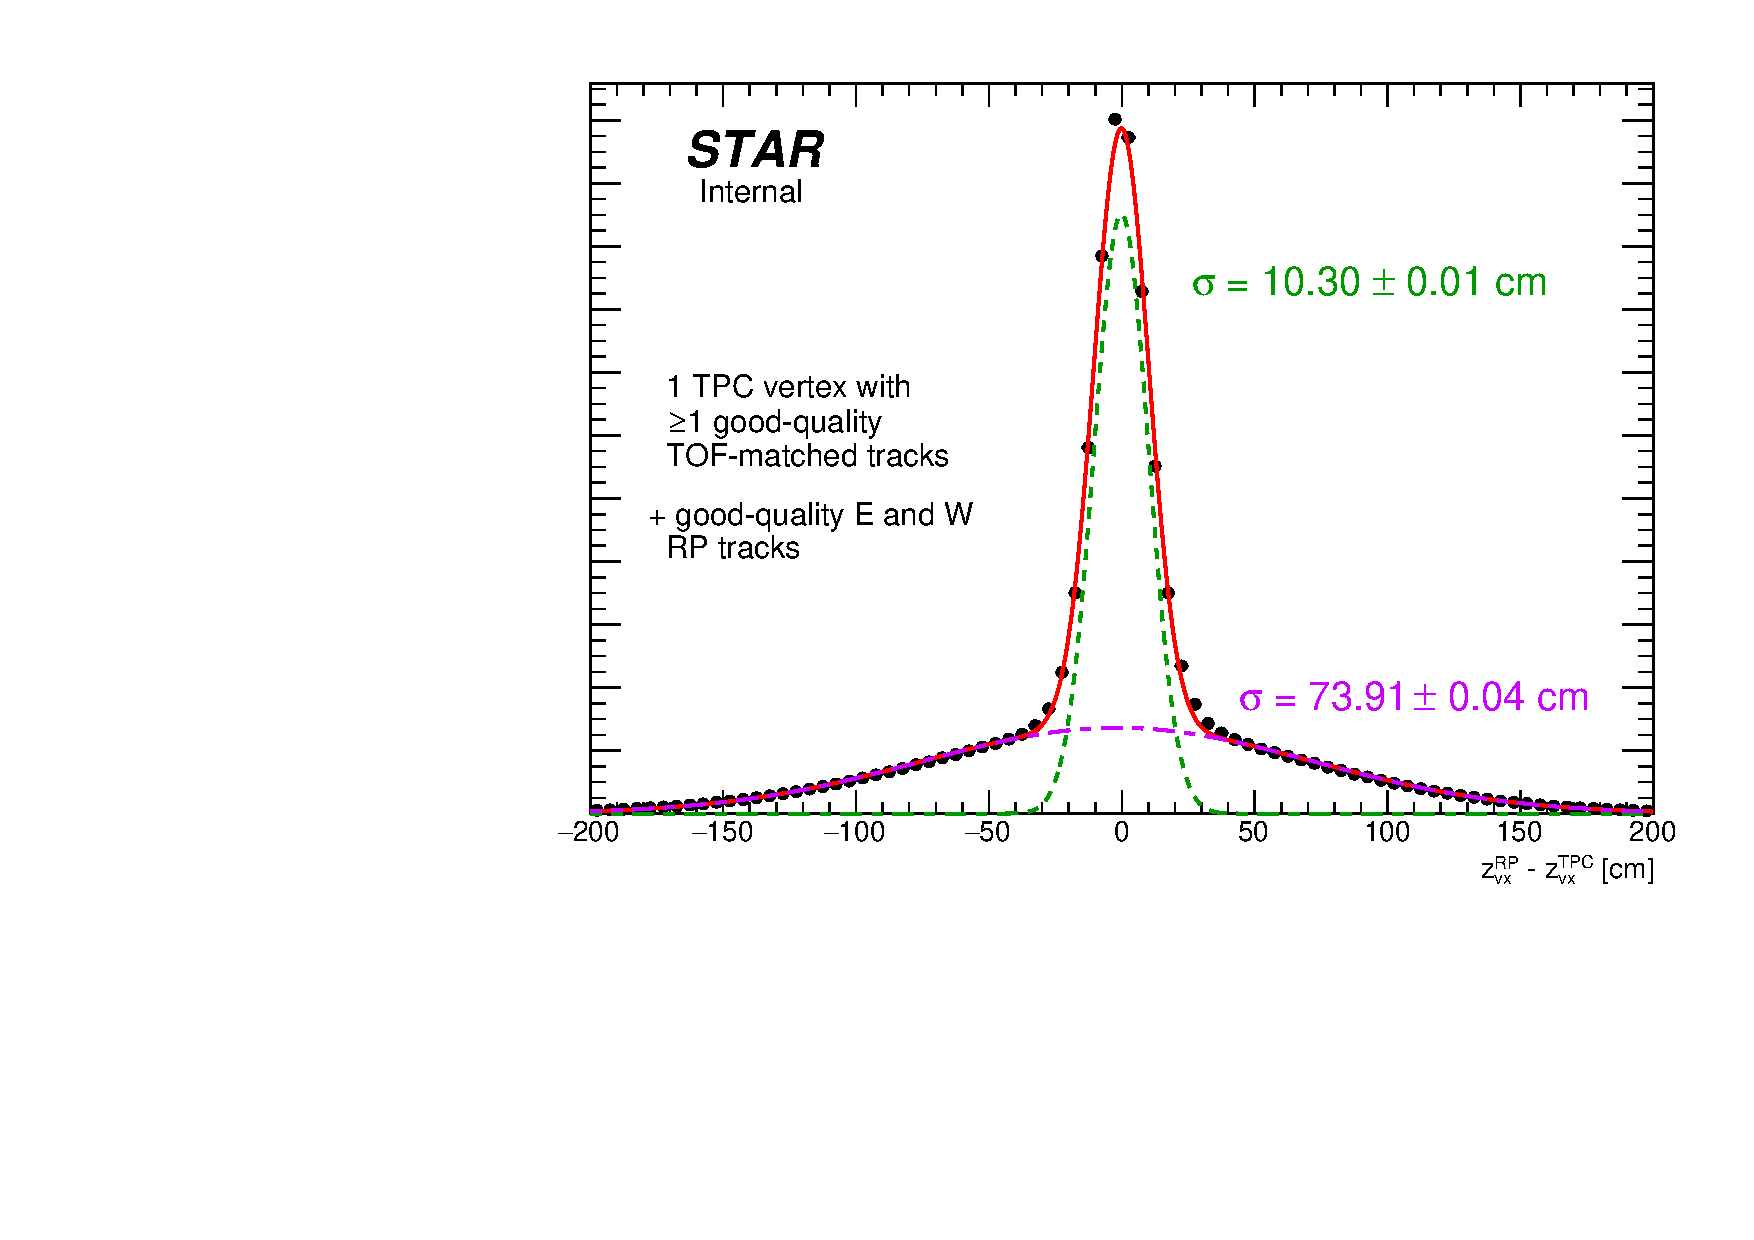
\includegraphics[width=\linewidth]{graphics/eventSelection/zVertexRpMinusZVertexTpc.pdf}}}
  \end{subfigure}
}%
\caption[Correlation and difference of $z$-vertex position measured in Roman Pots and TPC.]{Correlation (Fig.~\ref{fig:zVertexRpVsTpc}) and difference (Fig.~\ref{fig:zVertexRpMinusZVertexTpc}) of $z$-vertex position measured in Roman Pots and TPC in RP\_CPT2 triggers, after preselection described in the plots.}\label{fig:zVertexRpTpc}
\end{figure}%
%---------------------------
The sum of two Gaussian distributions was fitted to data in Fig.~\ref{fig:zVertexRpMinusZVertexTpc} yielding good description of the distribution of $\Delta z_{\text{vtx}}$ with the width parameters equal $10.3$~cm (CD signal) and $73.9$~cm (pile-up). The first parameter reflects the time resolution of RPs (the $z_{\text{vtx}}^{\text{RP}}$ measurement), as the TPC resolution is much better ($\sim 1$~cm). Value of the second parameter, consistent with $\sqrt{2}\sigma_{z_{\text{vtx}}}\approx\sqrt{2}\cdot52~\text{cm}\approx 73.5$~cm, confirms that the wide distribution under the narrow signal peak is uncorrelated background, in other words forward protons originating from a different vertex than the central tracks. To reject this background without significant loss of the signal, we introduce $3.5\sigma_{\Delta z_{\text{vtx}}}$ cut on $\Delta z_{\text{vtx}}$.


% %---------------------------
% \begin{figure}[ht!]
% % \begin{wrapfigure}{l}{0.475\textwidth}%[ht!]
% \centering%
% 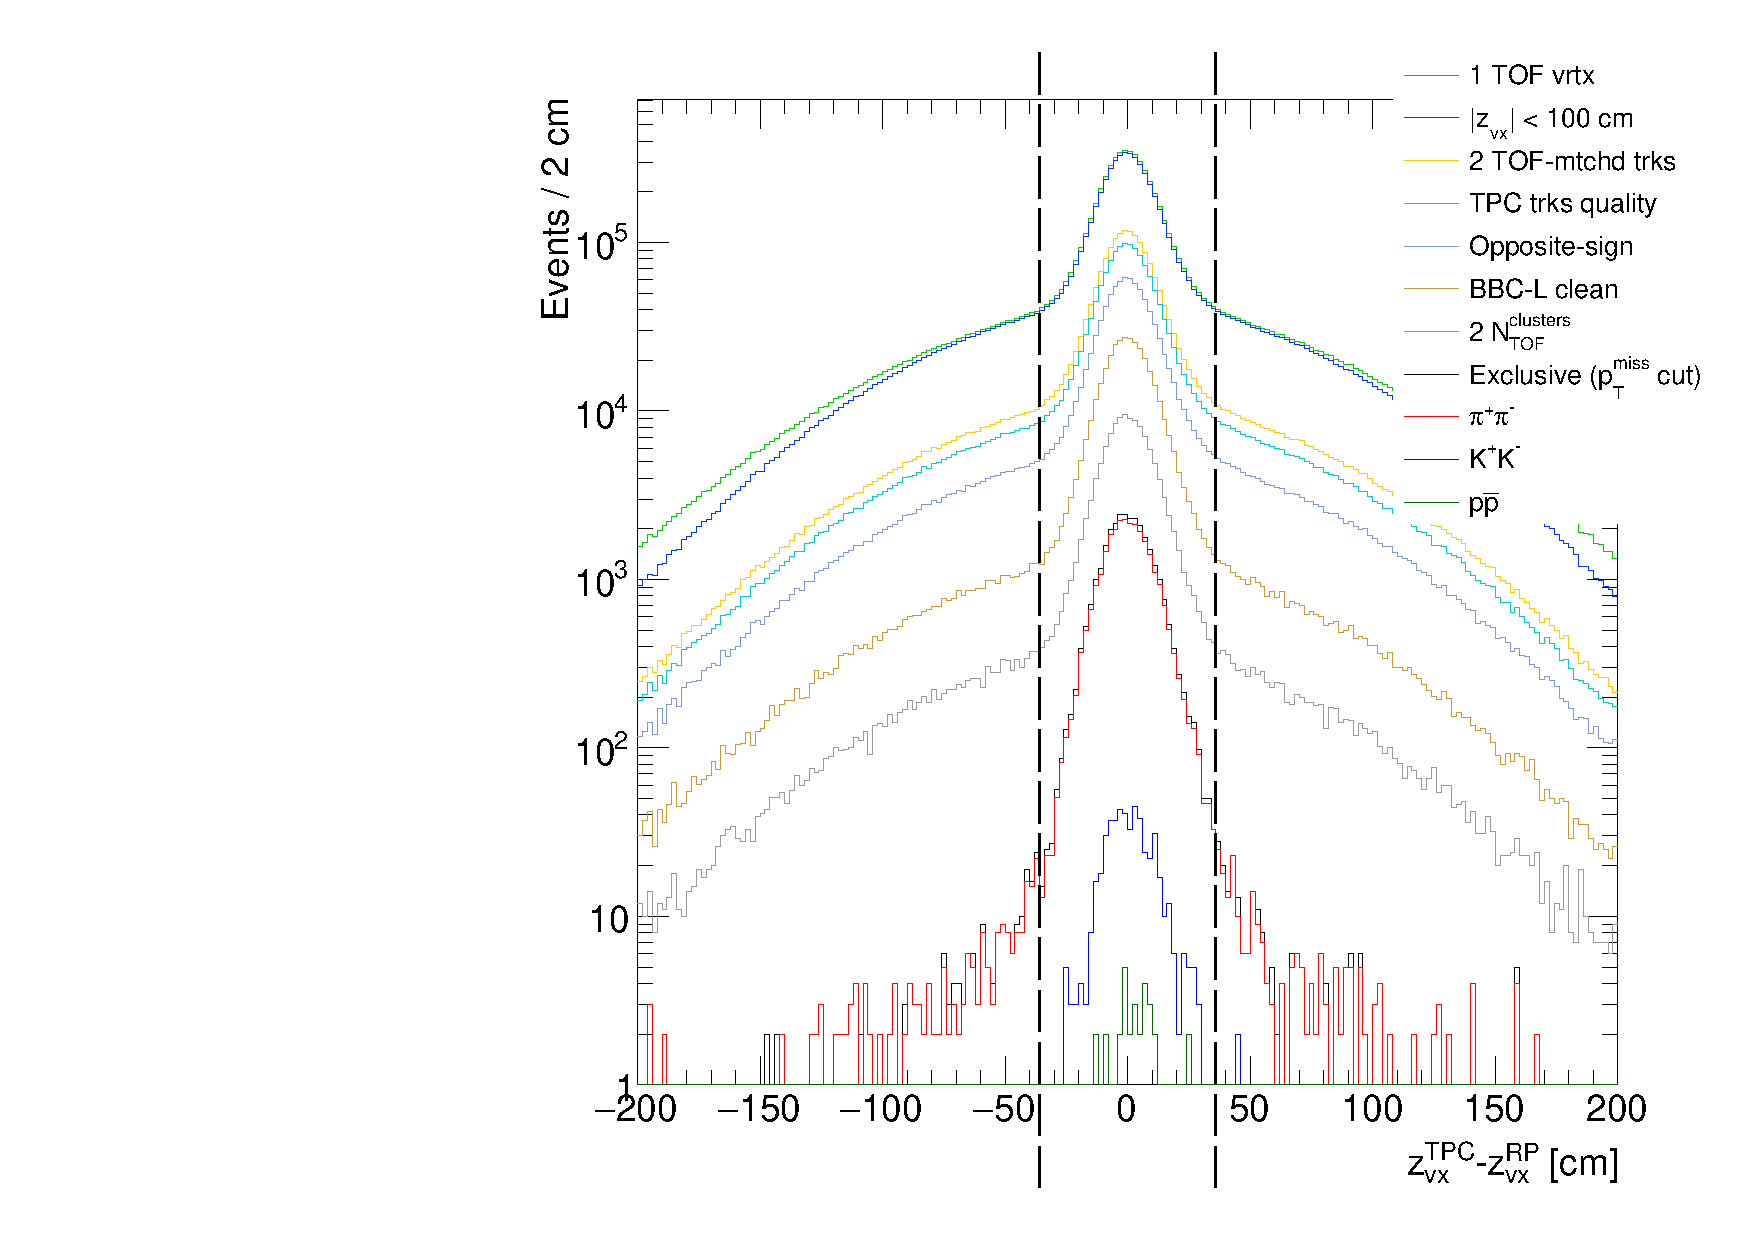
\includegraphics[width=0.475\linewidth,page=1]{graphics/eventSelection/DeltaZVx.pdf}%
% % % 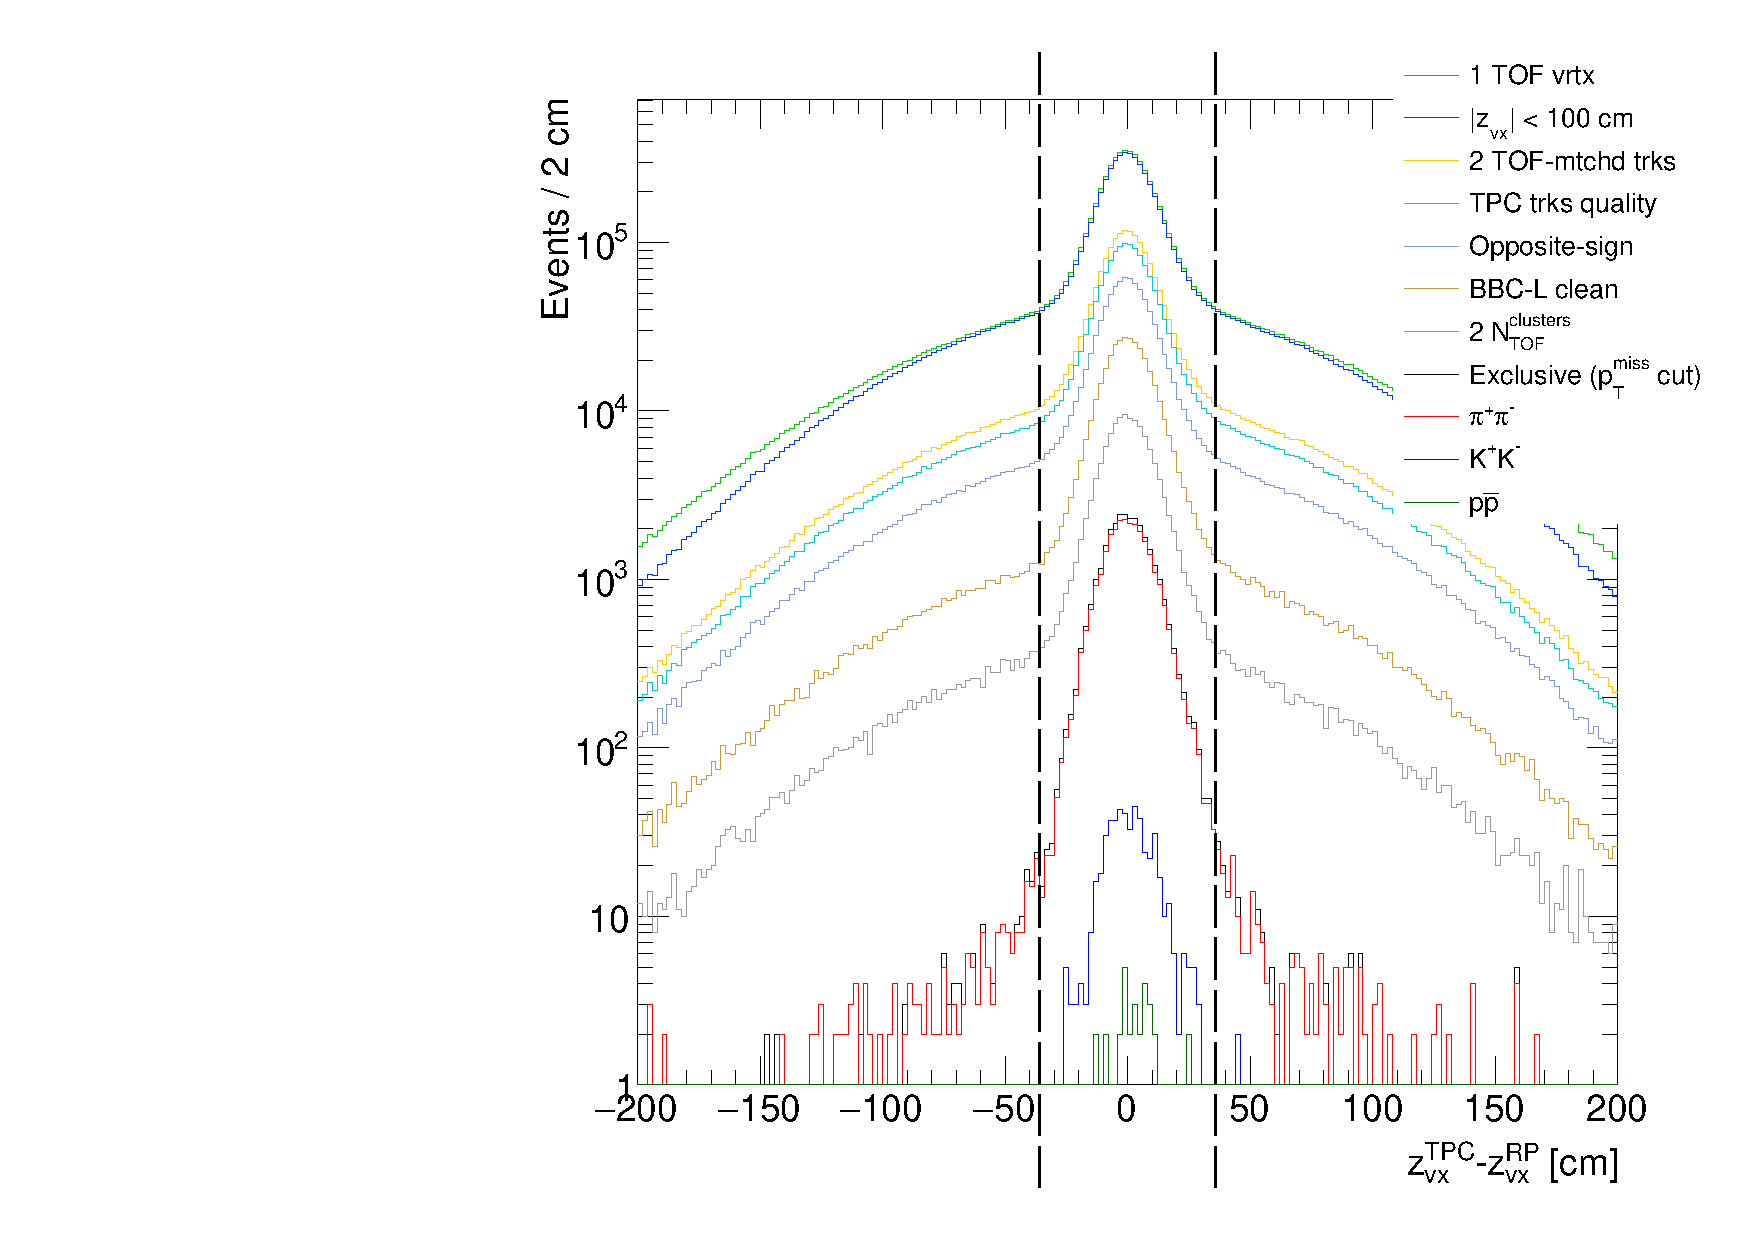
\includegraphics[width=\linewidth,page=1]{graphics/eventSelection/DeltaZVx.pdf}%
% \caption{Delta z-vx.}\label{fig:DeltaZVx}%
% \end{figure}
% % \end{wrapfigure}
% %---------------------------
%%%%%%%%%%%%%%%%%%%%%%%%%%%%%%%%%%%%%%%%%%%%%%%%%%%%%%%%%%%%%%%%%%%%%%%%%%%%%%%%%%%%%%%%%%%%%%%%%%%%%%%%%%%%%%%%%%%%%%%%%%%%%%%%%%%%




%%%%%%%%%%%%%%%%%%%%%%%%%%%%%%%%%%%%%%%%%%%%%%%%%%%%%%%%%%%%%%%%%%%%%%%%%%%%%%%%%%%%%%%%%%%%%%%%%%%%%%%%%%%%%%%%%%%%%%%%%%%%%%%%%%%%
\subsection{(\ref{enum:CutBbcLarge})~BBC-large signal veto}\label{sec:C6}

At the trigger level a veto on signal in small BBC detectors was used. During offline analysis we found that the non-exclusive background can be reduced if an additional veto on signal in large BBC detectors is added. It is connected with the fact that vast majority of selected RP\_CPT2 triggers were from the central diffraction process to which CEP belongs. Many of central diffraction events have particles produced in the rapidity region outside the TPC and TOF acceptance, some hitting large BBC tiles. Presence of signal in large BBC is therefore a signature of background or a pile-up interaction.

The response of large BBC tiles is different from that of small BBC tiles, as shown in sample plots in Fig.~\ref{fig:sampleBbcResponse} (similar distributions for all channels can be found in Appendix~\ref{appendix:bbc}). Typically in small BBC tiles a peak visible in ADC distribution around $100-150$ (Figs.~\ref{fig:sampleBbcSmallAdcVsTac},\ref{fig:sampleBbcSmallAdc}), a signature of good separation of the electronics noise and signal from the ionizing particle. No such feature is observed in corresponding distribution for large BBC tile (Figs.~\ref{fig:sampleBbcLargeAdcVsTac},\ref{fig:sampleBbcLargeAdc}), which can be explained by the difference in geometry (in size) of small and large tiles. In large BBC tiles the path that scintillation light must travel to reach PMT is much longer in comparison to smal BBC tiles (multiple reflections on the main tile surface due to small thickness of the tile) therefore it is highly attenuated and extended in time. This is possible reason of lack of signal peak in the ADC distribution in large BBC tile spectrum (Fig.~\ref{fig:sampleBbcLargeAdc}), as well as the late-TAC (TAC$<\sim600$, ADC$<100$) tail in the ADC vs. TAC spectrum (slewing effect, Fig.~\ref{fig:sampleBbcLargeAdcVsTac}). Nevertheless, the above features of BBC-large response does not disqualify this detector from being used as a veto detector, as in this case lower efficiency of the detector only reduce the background rejection power.


%---------------------------
\begin{figure}%[h]
\centering
\parbox{0.4725\textwidth}{
  \centering
  \begin{subfigure}[b]{\linewidth}
                \subcaptionbox{\label{fig:sampleBbcSmallAdcVsTac}}{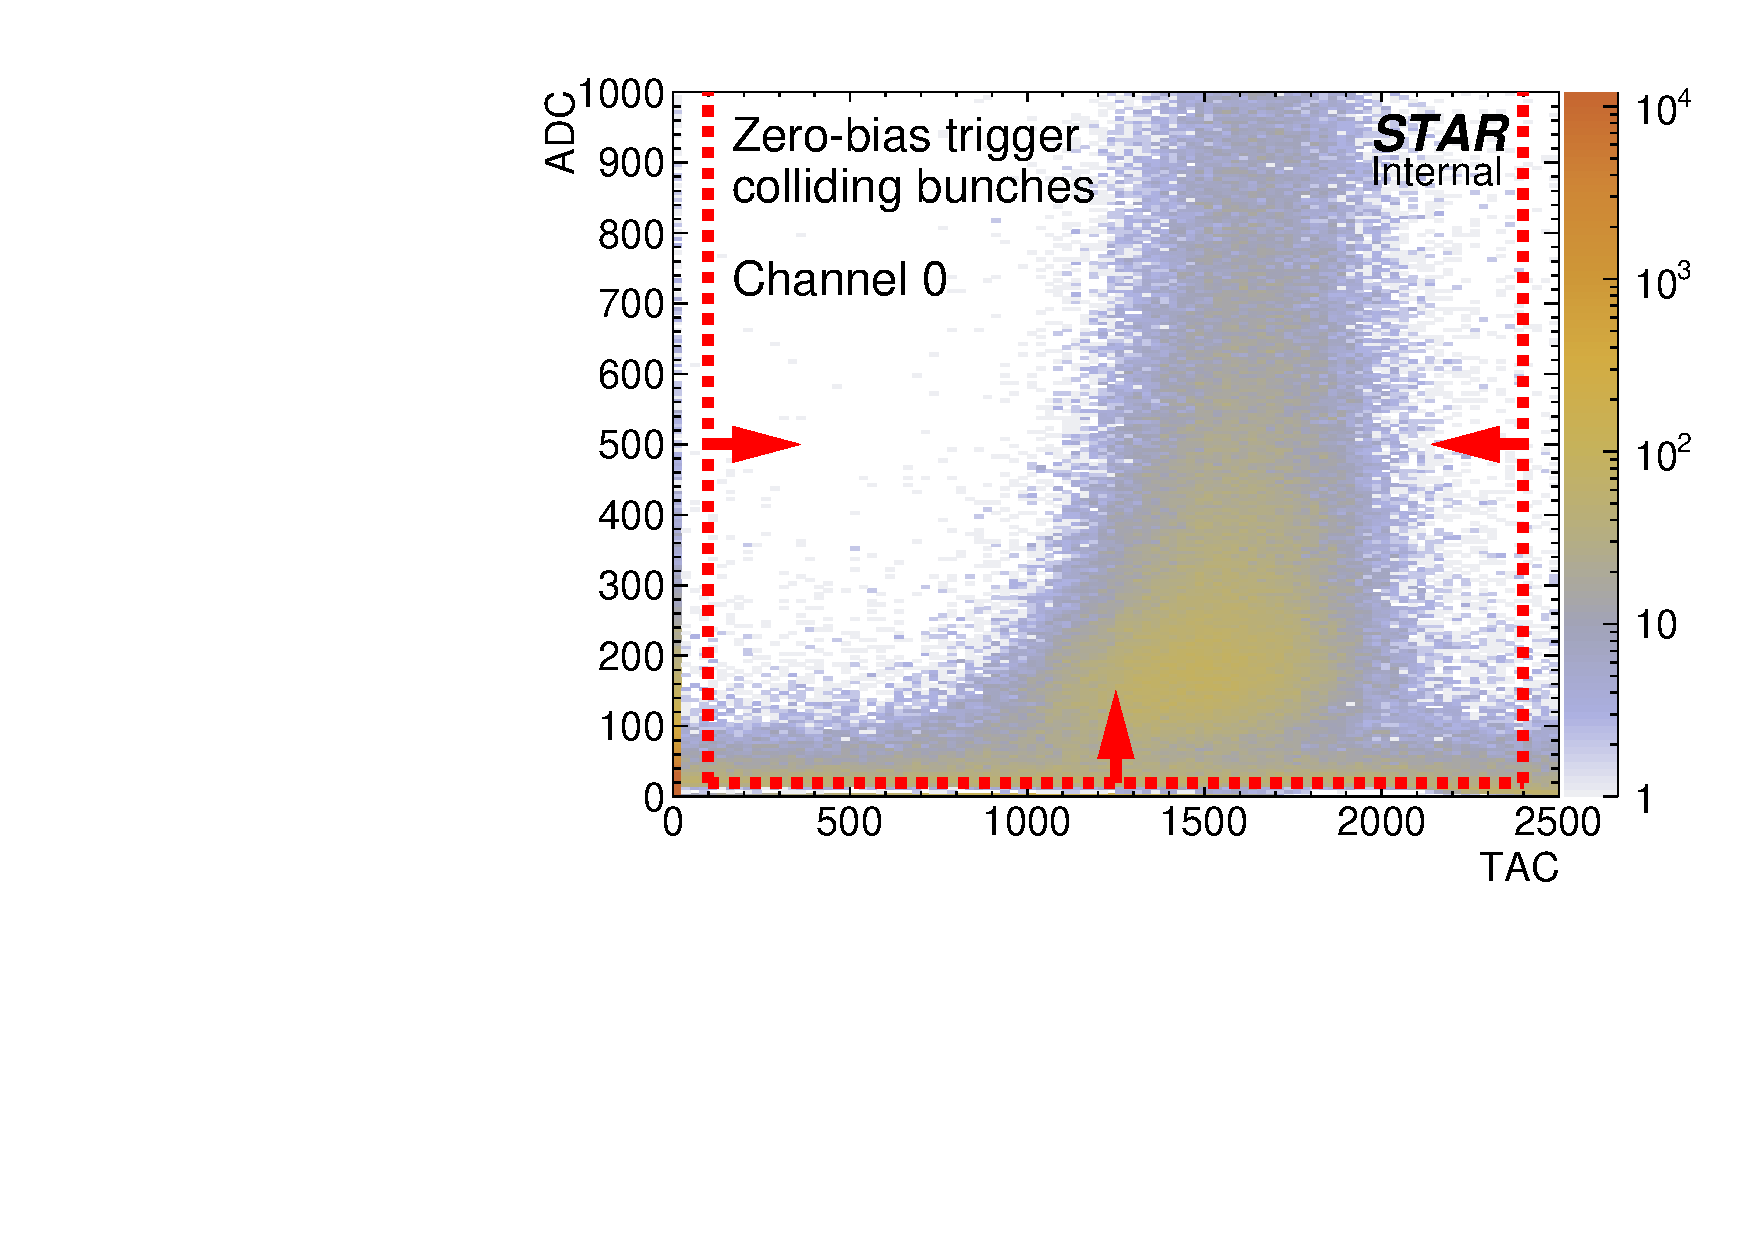
\includegraphics[width=\linewidth,page=1]{graphics/eventSelection/bbc/Bbc_ADCvsTAC_collidingBunches.pdf}}
  \end{subfigure}\\
  \begin{subfigure}[b]{\linewidth}\addtocounter{subfigure}{1}
                \subcaptionbox{\label{fig:sampleBbcSmallAdc}}{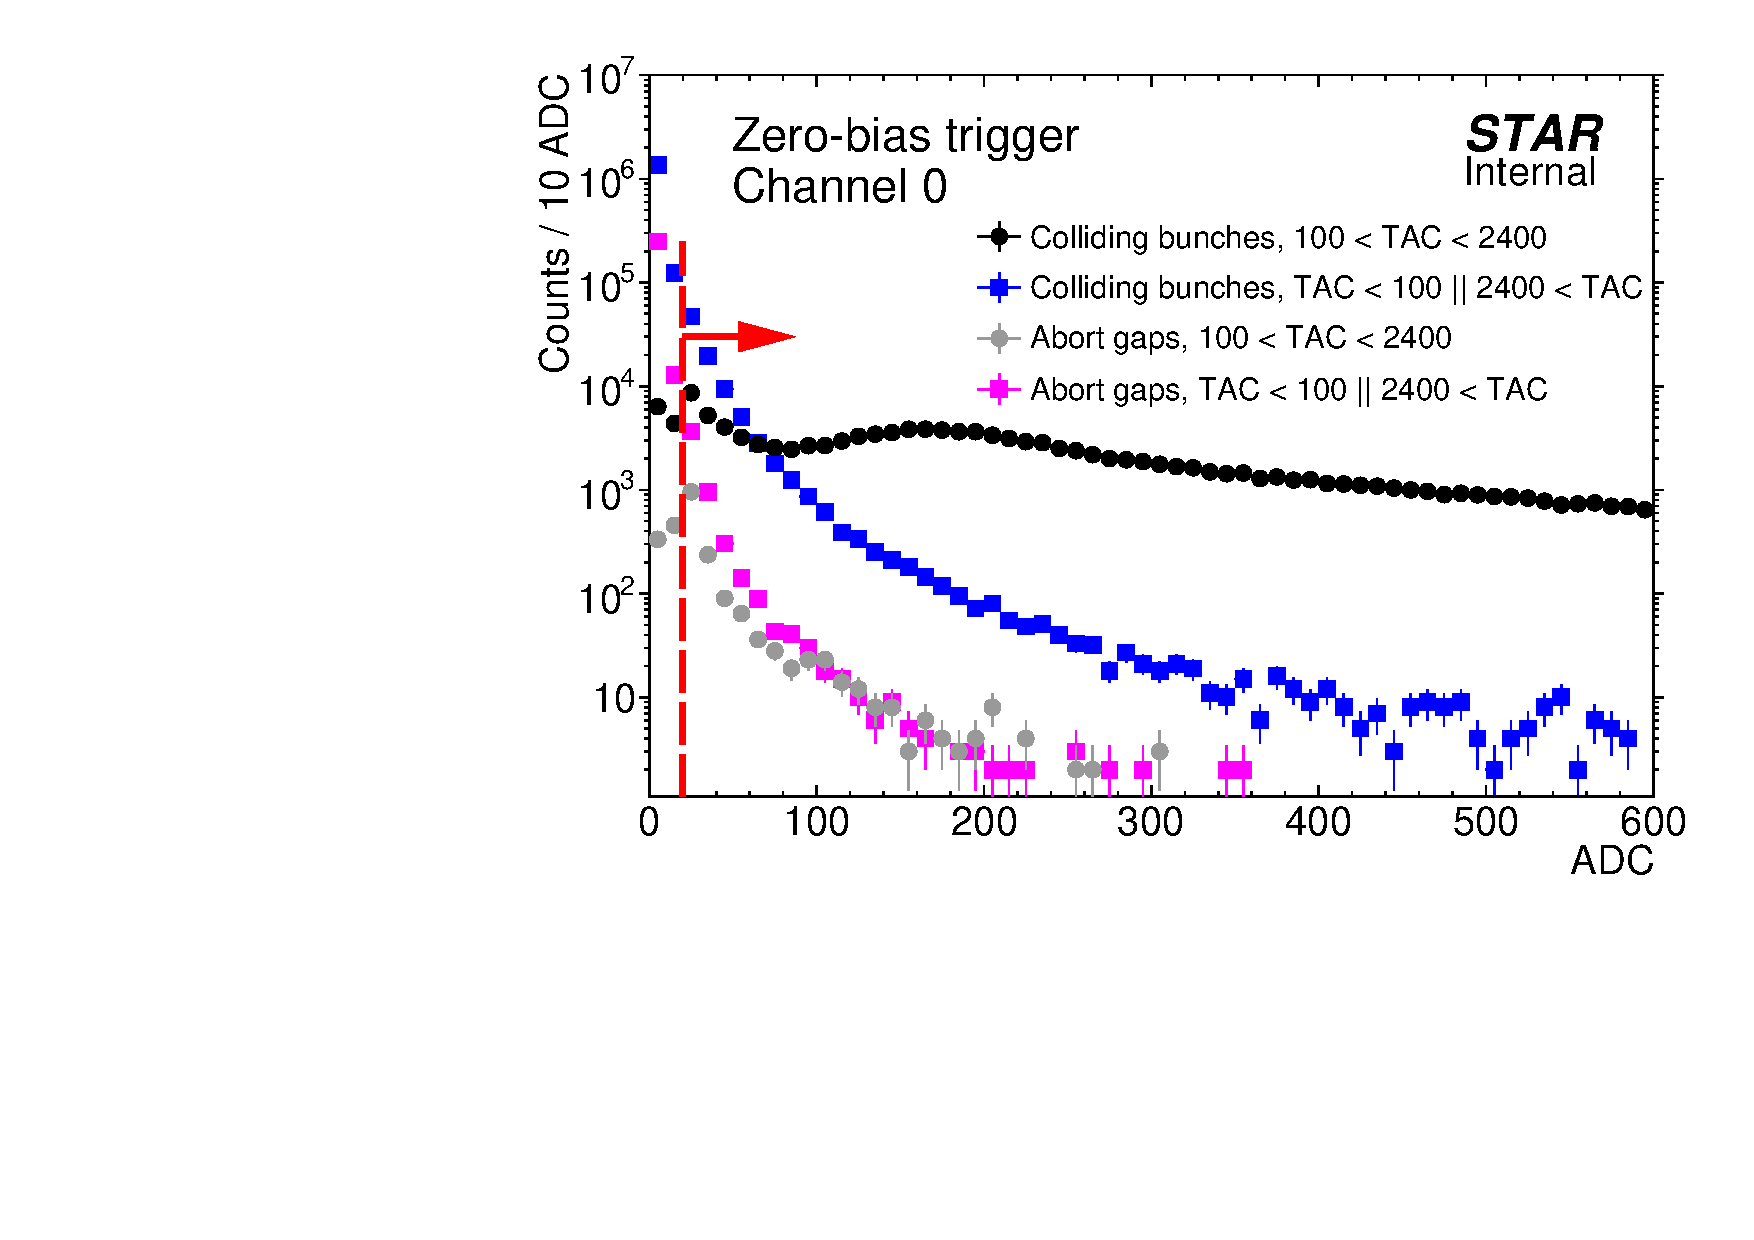
\includegraphics[width=\linewidth,page=1]{graphics/eventSelection/bbc/Bbc_ADC.pdf}}
  \end{subfigure}
}%
\quad\quad%
\parbox{0.4725\textwidth}{
  \centering
  \begin{subfigure}[b]{\linewidth}\addtocounter{subfigure}{-2}
                \subcaptionbox{\label{fig:sampleBbcLargeAdcVsTac}}{\includegraphics[width=\linewidth,page=17]{graphics/eventSelection/bbc/Bbc_ADCvsTAC_collidingBunches.pdf}}
  \end{subfigure}\\
  \begin{subfigure}[b]{\linewidth}\addtocounter{subfigure}{1}
                \subcaptionbox{\label{fig:sampleBbcLargeAdc}}{\includegraphics[width=\linewidth,page=17]{graphics/eventSelection/bbc/Bbc_ADC.pdf}}
  \end{subfigure}
}%
\caption[Sample BBC-small and BBC-large response in zero-bias triggers.]{Sample BBC-small (left column) and BBC-large (right column) response in zero-bias data. Top row shows TAC vs. ADC distributions, bottom row shows projection of the corresponding two-dimensional ditribution on $x$-axis (ADC) in the TAC range quoted in the legend, for both abort gaps and colliding bunches. Red lines and arrows indicate thresholds for a signal in presented channels.}\label{fig:sampleBbcResponse}
\end{figure}
%---------------------------


Each channel of the BBC-large has different response to signal from ionizing particle, as well as different level of noise. We decided to set up a signal threshold for each channel based on a study of the noise in abort gaps (in zero-bias data). This noise, in principle, should be solely the electronics noise. We checked for each channel the probability to detect a signal with ADC above certain threshold and with TAC contained within 100 and 2400 (the same window is deafult for small BBC). The result is shown in Fig.~\ref{fig:bbcLargeThresholds}. Next, we established final ADC thresholds in each BBC-large channel by requiring that the noise in BBC-large would cause a veto in maximally $3.5\%$ of events. Such number was chosen because it was consistent with an average ADC threshold of 40, found optimal in terms of selection efficiency and sample purity (see Appendix~\ref{appendix:workingPoint}), as well as it was acceptably low. To transform it to $\text{ADC}_{thr}$ we first assumed that the noise is uncorrelated between the channels. With this assumption one can connect the probability of the veto in whole BBC-large detector (east and west) caused by noise $\mathcal{P}_{\text{veto}}^{\text{noise}}$ with the probability of the signal induced by noise in single BBC-large channel $\mathcal{P}_{i,\text{sig}}^{\text{noise}}$:
\begin{equation}\label{eq:bbcNoise1}
 \mathcal{P}_{\text{veto}}^{\text{noise}} = 1-\mathcal{P}_{!\text{veto}}^{\text{noise}} = 1-\left( 1-\mathcal{P}_{i,\text{sig}}^{\text{noise}} \right)^{N^{\text{BBC}}_{\text{ch}}}.
\end{equation}
In the equation above $N^{\text{BBC}}_{\text{ch}}$ denotes number of active channels in BBC-large. From plots contained in Appendix~\ref{appendix:bbc} one can read that there were 14 active channels in BBC-large. 2 dead channels were found on the west side (40 and 42). By transforming Eq.~\ref{eq:bbcNoise1} to the form presented below we can calculate the threshold probability for a single BBC-large channel:
\begin{equation}\label{eq:bbcNoise2}
 \mathcal{P}_{i,\text{sig}}^{\text{noise}} = 1-\sqrt[N^{\text{BBC}}_{\text{ch}}]{1-\mathcal{P}_{\text{veto}}^{\text{noise}}} = 1-\sqrt[14]{1-0.035} \approx 0.0025.
\end{equation}
In the last step we translated this number to ADC threshold for each channel of BBC-large. For this purpose we used Fig.~\ref{fig:bbcLargeThresholds}. The $x$-axis projection of the crossing point of each color line with the $y$-axis value of 0.0025 defines $\text{ADC}_{thr}$ for each particular channel. These numbers are listed in Tab.~\ref{tab:bbcLargeThresholds}. The event was dropped from analysis if any of the BBC-large channels registered signal of strength $\text{ADC}_{i}>\text{ADC}_{i,thr}$ and $100<\text{TAC}_{i}<2400$.



\begin{table}%[h]
	\begin{minipage}{0.65\linewidth}
		\centering
		\includegraphics[width=\linewidth]{graphics/eventSelection/bbc/BbbLargeThreshold.pdf}
		\captionof{figure}[Probability of false BBC-large signal (noise-induced).]{Percentage of events in abort gaps from zero-bias triggers with the ADC counts larger than the ADC threshold given in the $x$-axis, for each BBC-large channel. Measured points with statistical uncertainties are connected with a smooth line of corresponding color for better visualization.}
		\label{fig:bbcLargeThresholds}
	\end{minipage}\hfill
	\begin{minipage}{0.3\linewidth}
		\centering
		\begin{tabular}{c|c||c|c}
			\multicolumn{2}{c||}{East} & \multicolumn{2}{c}{West} \\ \hline
			$i$  & $\text{ADC}_{\text{thr}}$ & $i$  & $\text{ADC}_{\text{thr}}$ \\ \hline
			16 & 27 & 40 & (dead) \\
			17 & 30 & 41 & 31 \\
			18 & 26 & 42 & (dead) \\
			19 & 37 & 43 & 14 \\
			20 & 25 & 44 & 29 \\
			21 & 55 & 45 & 30 \\
			22 & 43 & 46 & 33 \\
			23 & 27 & 47 & 22 \\
		\end{tabular}
		\caption[Offline ADC thresholds in BBC-large.]{Offline ADC thresholds in BBC-large.\newline\newline\newline\newline\newline\newline\newline\newline}
		\label{tab:bbcLargeThresholds}
	\end{minipage}

\end{table}

Observation of high purification of CEP sample with described BBC-large veto in the data from run 15 was helpful to improve the CEP trigger for run 17. The improved trigger called RP\_CPT2noBBCL was similar to RP\_CPT2 with an addition of BBC-large veto using ADC threshold of 50.

%%%%%%%%%%%%%%%%%%%%%%%%%%%%%%%%%%%%%%%%%%%%%%%%%%%%%%%%%%%%%%%%%%%%%%%%%%%%%%%%%%%%%%%%%%%%%%%%%%%%%%%%%%%%%%%%%%%%%%%%%%%%%%%%%%%%



%%%%%%%%%%%%%%%%%%%%%%%%%%%%%%%%%%%%%%%%%%%%%%%%%%%%%%%%%%%%%%%%%%%%%%%%%%%%%%%%%%%%%%%%%%%%%%%%%%%%%%%%%%%%%%%%%%%%%%%%%%%%%%%%%%%%
\subsection{(\ref{enum:CutTofClusters})~TOF clusters limit}\label{sec:C7}

The TOF is mainly used to distinguish real TPC tracks from the fakes, as well as it helps to identify particles. However, we also used it to reject non-CEP events in which the TPC tracks were not reconstructed or were not successfully matched to TOF hit. For this we introduced a concept of a TOF cluster - a group of offline TOF hits close in space and time. We expect that such cluster of hits is induced by the single primary particle, eventually associated with the secondaries (e.g. delta rays).

We define a TOF cluster as a group of reconstructed TOF hits with the ($\phi$, $\eta$) space distance $R$ to neighbouring hit (defined similarly to Eq.~\eqref{eq:etaPhiR} not larger than 0.1 and with the time distance to the same hit $\Delta t$ not larger than 1.5~ns. In other words, TOF clusters are formed by the offline hits that form at least one pair with the other hit in the cluster satisfying
\begin{equation}
 R<0.1,~~~~~~\Delta t<1.5~\text{ns}.
\end{equation}
Per event no more than 1 additional TOF cluster was allowed, thus in total the number of reconstructed TOF clusters $N^{\text{TOF}}_{\text{clstrs}}$ could not exceed 3.

%---------------------------
\begin{figure}[ht!]
% \begin{wrapfigure}{l}{0.475\textwidth}%[ht!]
\centering%
\includegraphics[width=0.475\linewidth,page=1]{graphics/eventSelection/NTofClusters.pdf}%
% % \includegraphics[width=\linewidth,page=1]{graphics/eventSelection/NTofClusters.pdf}% 
\caption{NTofClusters.}\label{fig:NTofClusters}%
\end{figure}
% \end{wrapfigure}
%---------------------------

\subsection{(\ref{enum:CutPid})~Particle identification}\label{subsec:pidCuts}\label{sec:C8}

Particles were identified using combined information from the TPC ($dE/dx$) and TOF (time of hit detection in the TOF subsystem). Merging informations from two sources led to reduction of misidentifications, as well as gave access to higher kaon and proton momentum range where $dE/dx$ of different species overlap.

Compatibility of track $dE/dx$ with that expected from particle of type $X$ was determined using the quantity $n\sigma_{X}$ widely used at STAR, defined as
\protect \begin{equation}\label{eq:nSigmaDef} n\sigma_{X} =  \ln{\left[(dE/dx)^\text{measured} / (dE/dx)_{X}^\text{theory}\right]}~~/~~\sigma_{dE/dx}, \end{equation}
%
where $(dE/dx)^\text{measured}$ is the ionization energy loss of the TPC track, $(dE/dx)_{X}^\text{theory}$ is the Bethe-Bloch~\cite{Bichsel} expectation for the given particle type ($X=\pi$, $K$, $p$) at reconstructed track momentum, and $\sigma_{dE/dx}$ is the statistical uncertainty of $\ln{(dE/dx)^\text{measured}}$. Quantity $n\sigma_{X}$ is in fact a pull: $(dE/dx)^\text{measured}$ is (in first order) an average over $\text{Landau}\otimes\text{normal}$-distributed $dE/dx$ of single TPC hits forming the track, hence the $(dE/dx)^\text{measured}$ is distributed log-normally and $\ln{(dE/dx)^\text{measured}}$ - normally. From $n\sigma_{X}$ of the two tracks the $\chi^{2}$ statistic for a $XX$ pair hypothesis was calculated:
%
\begin{equation}\label{eq:chiSqDef}\chi^{2}_{dE/dx}(XX) = \left(n\sigma_{X}^{\text{trk1}}\right)^{2} + \left(n\sigma_{X}^{\text{trk2}}\right)^{2}.\end{equation}
%
Sometimes we also quote $n\sigma^{\text{pair}}$ quantity (which is no longer a Gaussian pull) connected with $\chi^{2}$ through relation
%
\begin{equation}\label{eq:nSigmaPairDef}n\sigma^{\text{pair}}_{X} = \sqrt{\chi^{2}_{dE/dx}(XX)} = \sqrt{\left(n\sigma_{X}^{\text{trk1}}\right)^{2} + \left(n\sigma_{X}^{\text{trk2}}\right)^{2}}.\end{equation}
%
The time of detection of particle in the TOF system was used to reconstruct its squared mass $m^{2}_{\text{TOF}}$. For this purpose the time of primary interaction is typically used (''start time``), reconstructed by detecting fragments of dissociated beam particles in VPD detectors on both sides of the interaction point\footnote{Time measured from protons in the RP detectors cannot be used because RP readout runs on independent clock from that used by VPD and TOF.}. However, it is not accessible in CEP as the initial protons survive the interaction intact. We therefore assumed that both central tracks are of the same type which is natural expectation for CEP events. With this assumption the time difference between TOF hits and measured tracks' momenta and lengths of helical paths between the primary vertex and TOF then allow to calculate $m^{2}_{\text{TOF}}$. The derivation of formula used to obtain $m^{2}_{\text{TOF}}$ is presented in Appendix~\ref{appendix:squaredMass}.

Particle identification involved a few steps. First, the $pp$ hypothesis was verified:
\begin{equation}\label{eq:pidPPbar}\lefteqn{\overbrace{\phantom{\chi^{2}_{dE/dx}(pp)<9\;\;\; \& \;\;\; m^{2}_{\text{TOF}} > 0.6~\mbox{GeV}^{2}}}^{\text{likely}~pp}}\chi^{2}_{dE/dx}(pp)<9\;\;\; \& \;\;\; \underbrace{m^{2}_{\text{TOF}} > 0.6~\mbox{GeV}^{2}\;\;\; \& \;\;\; \chi^{2}_{dE/dx}(\pi\pi)>9\;\;\; \& \;\;\; \chi^{2}_{dE/dx}(KK)>9}_{\text{unlikely}~\pi\pi~\text{or}~KK}.\end{equation}
If any of above was not satisfied, the pair was checked for compatibility with $KK$ hypothesis:
%
\begin{equation}\label{eq:pidKK}%
\lefteqn{\overbrace{\phantom{\chi^{2}_{dE/dx}(KK)<9\;\;\; \& \;\;\; m^{2}_{\text{TOF}} > 0.15~\mbox{GeV}^{2}}}^{\text{likely}~KK}}\chi^{2}_{dE/dx}(KK)<9\;\;\; \& \;\;\; \underbrace{m^{2}_{\text{TOF}} > 0.15~\mbox{GeV}^{2}\;\;\; \& \;\;\; \chi^{2}_{dE/dx}(\pi\pi)>9}_{\text{unlikely}~\pi\pi}\;\;\; \& \;\;\; \underbrace{\chi^{2}_{dE/dx}(pp)>9}_{\text{unlikely}~pp}.
\end{equation}
%
In case the pair was neither recognized as $p\bar{p}$ or $K^{+}K^{-}$, it was assumed to be a $\pi^{+}\pi^{-}$ pair if the $dE/dx$ of positive and negative charge track was consistent with pion hypothesis at $3\sigma$ level:
\begin{equation}\label{eq:pidPiPi}|n\sigma_{\pi}^{\text{trk1}}|<3\;\;\; \& \;\;\; |n\sigma_{\pi}^{\text{trk2}}|<3.\end{equation}




\begin{figure}[h]
\centering
\parbox{0.4725\textwidth}{
  \centering
  \begin{subfigure}[b]{\linewidth}
                \subcaptionbox{\label{fig:SqRootNSigma2D_a}}{\includegraphics[width=1.05\linewidth,page=1]{graphics/eventSelection/pid/PidSelector_SqRootNSigma2D.pdf}}
  \end{subfigure}\\
  \begin{subfigure}[b]{\linewidth}\addtocounter{subfigure}{1}
                \subcaptionbox{\label{fig:SqRootNSigma2D_c}}{\includegraphics[width=1.05\linewidth,page=3]{graphics/eventSelection/pid/PidSelector_SqRootNSigma2D.pdf}}
  \end{subfigure}
}%
\quad\quad%
\parbox{0.4725\textwidth}{
  \centering
  \begin{subfigure}[b]{\linewidth}\addtocounter{subfigure}{-2}\vspace*{-13pt}
                \subcaptionbox{\label{fig:SqRootNSigma2D_b}}{\includegraphics[width=1.05\linewidth,page=2]{graphics/eventSelection/pid/PidSelector_SqRootNSigma2D.pdf}}
  \end{subfigure}\\
  \begin{minipage}[t][1.042\linewidth][t]{\linewidth}\vspace{10pt}
    \caption[$n\sigma^{\text{pair}}_{X}$ vs. $n\sigma^{\text{pair}}_{Y}$.]{Two-dimensional distributions of $n\sigma^{\text{pair}}_{\pi}$ vs.~$n\sigma^{\text{pair}}_{K}$ (\subref{fig:SqRootNSigma2D_a}), $n\sigma^{\text{pair}}_{\pi}$ vs.~$n\sigma^{\text{pair}}_{p}$  (\subref{fig:SqRootNSigma2D_b}) and $n\sigma^{\text{pair}}_{K}$ vs.~$n\sigma^{\text{pair}}_{p}$  (\subref{fig:SqRootNSigma2D_c}) for exclusive event candidates after full event selection except PID cuts (except cuts~\ref{enum:CutPid}). Dashed lines indicate the value of $n\sigma^{\text{pair}}$ which is used in pair identification~\ref{enum:CutPid} ($n\sigma^{\text{pair}}_{X}=9$ which is equivalent to $\chi^{2}(XX)=9$).}\label{fig:SqRootNSigma2D}
  \end{minipage}
}%

\end{figure}
%--------------------------- 


In Fig.~\ref{fig:SqRootNSigma2D} we present two-dimensional distributions of $n\sigma^{\text{pair}}$ variables which help better undestand the behaviour and aim of $n\sigma^{\text{pair}}$ ($\chi^{2}$) cuts in Eqs.~\eqref{eq:pidPPbar}, \eqref{eq:pidKK}. Regions of enriched population of specific pair species are appropriately labeled. Similar connections between $n\sigma^{\text{pair}}$ and $m^{2}_{\text{TOF}}$ are shown in Fig.~\ref{fig:mSqVsNSigmaPair}.
 

 
\begin{figure}[ht!]
  \centering
  \begin{tabular}{@{}p{0.47\linewidth}@{\quad\quad}p{0.47\linewidth}@{}}
    \subfigimg[width=\linewidth,page=1]{~~~~~~~~~~~a)}{graphics/eventSelection/pid/PidSelector_SqMassTofVsSqRootNSigma_pion.pdf} &
    \subfigimg[width=\linewidth,page=1]{~~~~~~~~~~~c)}{graphics/eventSelection/pid/SqMassTofVsSqRootNSigma_pion.pdf} \\[-10pt]
    \subfigimg[width=\linewidth,page=1]{~~~~~~~~~~~d)}{graphics/eventSelection/pid/PidSelector_SqMassTofVsSqRootNSigma_kaon.pdf} &
    \subfigimg[width=\linewidth,page=1]{~~~~~~~~~~~f)}{graphics/eventSelection/pid/SqMassTofVsSqRootNSigma_kaon.pdf} \\[-10pt]
    \subfigimg[width=\linewidth,page=1]{~~~~~~~~~~~g)}{graphics/eventSelection/pid/PidSelector_SqMassTofVsSqRootNSigma_proton.pdf} &
    \subfigimg[width=\linewidth,page=1]{~~~~~~~~~~~i)}{graphics/eventSelection/pid/SqMassTofVsSqRootNSigma_proton.pdf}    
  \end{tabular}\vspace*{-5pt}
  \caption[$n\sigma^{\text{pair}}_{X}$ vs. $m^{2}_{\text{TOF}}$.]{Two-dimensional distributions of $n\sigma^{\text{pair}}_{\pi}$ (top row), $n\sigma^{\text{pair}}_{K}$ (middle row) and $n\sigma^{\text{pair}}_{p}$ (bottom row) vs. $m^{2}_{\text{TOF}}$. The left column contains all clean BBC-large events with single TOF vertex and two opposite sign TOF-matched tracks (passing cuts~\ref{enum:CutPrimVx}, \ref{enum:TpcTofMatched}, \ref{enum:TpcOppoSign} and~\ref{enum:CutBbcLarge}), which provides excellent statistics to see the signatures or pairs of specific ID. The right column cantains exclusive event candidates after full event selection except PID cuts (except cuts~\ref{enum:CutPid}). Dashed red line and arrow indicate the cut imposed on plotted quantities which are used to select exclusive pairs of given particle species (keep in mind that these are not the only cuts).}\label{fig:mSqVsNSigmaPair}
\end{figure}





\begin{figure}[ht!]
  \centering
  \begin{tabular}{@{}p{0.49\linewidth}@{\quad}p{0.49\linewidth}@{}}
    \subfigimg[width=\linewidth,page=1]{~~~~~~~~~~~~~~~~~~~~~~~~~~~~~~~~~~~~~~~~~~~~~~~~~~~~~~~~~~~~~~a)}{graphics/eventSelection/pid/Chi2NSigma_pion.pdf} &
    \subfigimg[width=\linewidth,page=1]{~~~~~~~~~~~~~~~~~~~~~~~~~~~~~~~~~~~~~~~~~~~~~~~~~~~~~~~~~~~~~~c)}{graphics/eventSelection/pid/SqMassTof_pion.pdf} \\
    \subfigimg[width=\linewidth,page=1]{~~~~~~~~~~~~~~~~~~~~~~~~~~~~~~~~~~~~~~~~~~~~~~~~~~~~~~~~~~~~~~d)}{graphics/eventSelection/pid/Chi2NSigma_kaon.pdf} &
    \subfigimg[width=\linewidth,page=1]{~~~~~~~~~~~~~~~~~~~~~~~~~~~~~~~~~~~~~~~~~~~~~~~~~~~~~~~~~~~~~~f)}{graphics/eventSelection/pid/SqMassTof_kaon.pdf} \\
    \subfigimg[width=\linewidth,page=1]{~~~~~~~~~~~~~~~~~~~~~~~~~~~~~~~~~~~~~~~~~~~~~~~~~~~~~~~~~~~~~~g)}{graphics/eventSelection/pid/Chi2NSigma_proton.pdf} &
    \subfigimg[width=\linewidth,page=1]{~~~~~~~~~~~~~~~~~~~~~~~~~~~~~~~~~~~~~~~~~~~~~~~~~~~~~~~~~~~~~~i)}{graphics/eventSelection/pid/SqMassTof_proton.pdf}    
  \end{tabular}
  \caption[$\chi^{2}_{dE/dx}$ and $m^{2}_{\text{TOF}}$ for exclusive $\pi^+\pi^-$, $K^+K^-$ and $p\bar{p}$ candidates.]{Raw distributions of $\chi^{2}_{dE/dx}$ (left column) and $m^{2}_{\text{TOF}}$ (right column) for exclusive $\pi^+\pi^-$ (top row), $K^+K^-$ (middle row) and $p\bar{p}$ (bottom row) candidates after full event selection. Data are shown as black points, while stacked predictions for signal and backgrounds are shown as color histograms. Dashed red line and arrow indicate the value of cut imposed on plotted quantity to select exclusive pairs of given particle species. Last bins in each subfigure are overflows representing an integral of the tail of distribution. Presented distributions were obtained after all the cuts were applied, except the cut on presented quantity in the last step in PID algorithm used to select pairs of given species. Non-exclusive background was determined with a method described in Sec.~\ref{sec:nonExclBkgdDetermination}, while predictions for exclusive contributions were obtained as described in Sec.~\ref{sec:exclBkgdDetermination}.}\label{fig:pid_plots}
\end{figure}

%---------------------------------------------------------------------------------------------------------------

\subsection{(\ref{enum:CutMissingPt})~Exclusivity cut (missing \texorpdfstring{$p_{\text{T}}$}{pT} cut)}\label{subsec:ptMiss}\label{sec:C9}%

The most important cut which is used in this analysis to select events of exclusively produced pairs of particles is the missing transverse momentum, or the total transverse momentum cut. It benefits from detection and reconstruction of the forward proton in RP detectors - a rare capability among high energy physics experiments which STAR provides. The observable $p_{\text{T}}^{\text{miss}}$ used to select exclusive event is defined as
\begin{equation}\label{eq:missingPt}
 p_{\text{T}}^{\text{miss}} = \Big( \vec{p}_{p'}^{\hspace*{2pt}\text{E}} + \vec{p}_{h^{+}} + \vec{p}_{h^{-}} + \vec{p}_{p'}^{\hspace*{2pt}\text{W}} \Big)_{\text{T}} = \sqrt{\Big(p_{x}^{\text{miss}}\Big)^{2} + \Big(p_{y}^{\text{miss}}\Big)^{2}},
\end{equation}
with the other total momentum components defined analogously:\\
\begin{tabulary}{\textwidth}{LL}
\begin{equation}\label{eq:missingPx}
 p_{x}^{\text{miss}} = \Big( \vec{p}_{p'}^{\hspace*{2pt}\text{E}} + \vec{p}_{h^{+}} + \vec{p}_{h^{-}} + \vec{p}_{p'}^{\hspace*{2pt}\text{W}} \Big)_{x},
\end{equation}~~~~~~~~~~~~~~~~~~~~~
&
\begin{equation}\label{eq:missingPy}
 p_{y}^{\text{miss}} = \Big( \vec{p}_{p'}^{\hspace*{2pt}\text{E}} + \vec{p}_{h^{+}} + \vec{p}_{h^{-}} + \vec{p}_{p'}^{\hspace*{2pt}\text{W}} \Big)_{y}.
\end{equation}~~~~~~~~~~~~~~~~~~~~~
\end{tabulary}


Figure~\ref{fig:PxPyCentralTrksVsProtons} visualize the (anti-)correlation between the momentum components of the forward system (sum of two forward protons momenta) and the central system (sum of two central tracks momenta). The enhanced band at anti-diagonal restricted by dashed lines contains events balanced in momentum, a signature of exclusivity. Events outside this band are the non exclusive backgrounds, in most cases Central Diffraction events with some particles undected (due to detector inefficiency or produced outside acceptance). Slight horizontal enhancement in all distributions around $[\vec{p}^{\hspace*{2pt}\text{W}}_{p'}+\vec{p}^{\hspace*{2pt}\text{E}}_{p'}]_{x} = [\vec{p}^{\hspace*{2pt}\text{W}}_{p'}+\vec{p}^{\hspace*{2pt}\text{E}}_{p'}]_{x} =0$ is a signature of the elastic proton-proton scattering background with some non-elastic pile-up interaction which mimics the CEP event. All these backgrounds are reasonably low after the exclusivity cut, as described in Sec.~\ref{sec:nonExclBkgd}.

The momentum balance is shown one-dimensionally in Fig.~\ref{fig:MissingPxPy}, with the sum of $x$- and $y$-components of momentum shown repectively in the left and right column for each analyzed particle species. The sum of signal and background (both assumed to be described a Gaussian) was fitted to $p_{x}^{\text{miss}}$ and $p_{y}^{\text{miss}}$ distributions. Results of the fit are given in each subfigure. One can notice that the widths of Gaussian functions representing the exclusive signal are consistent among species and amount $\sigma_{p_{x}^{\text{miss}}}=27.4$~MeV for the $x$-component of total momentum, and $\sigma_{p_{y}^{\text{miss}}}=28.1$~MeV for the $y$-component of total momentum, taking the values of the lowest statistical uncertainty - for $\pi^{+}\pi^{-}$. These values are measures of the total momentum resolution respectively for $p_{x}^{\text{miss}}$ and $p_{y}^{\text{miss}}$. Having these number it is possible to form an elliptical on the missing momentum:

\begin{equation}\label{eq:ptMissEllipse}%
\left(\frac{p_{x}^{\text{miss}}}{\sigma_{p_{x}^{\text{miss}}}}\right)^{2} + \left(\frac{p_{y}^{\text{miss}}}{\sigma_{p_{y}^{\text{miss}}}}\right)^{2} < n_{\text{cut}}^{2}
\end{equation}
%
where $n_{\text{cut}}$ is the parameter denoting radius of limiting ellipsis in units of standard deviations of distributions of total momentum components (resolutions). Since these resolutions are nearly identical ($\sigma_{p_{x}^{\text{miss}}} = \sigma_{p_{y}^{\text{miss}}} = \sigma_{p_{x,y}^{\text{miss}}}$) such cut can be reduced (multiplying Ineq.~\ref{eq:ptMissEllipse} by $\sigma_{p_{x,y}^{\text{miss}}}^{2}$) to one-dimensional cut on a single quantity:

\begin{equation}%
\left(p_{x}^{\text{miss}}\right)^{2} + \left(p_{y}^{\text{miss}}\right)^{2} < \Big(n_{\text{cut}}\cdot\sigma_{p_{x,y}^{\text{miss}}}\Big)^{2}~~~~~~~\xrightarrow[~]{\sqrt{~}}~~~~~~~p_{\text{T}}^{\text{miss}} < n_{\text{cut}}\cdot\sigma_{p_{x,y}^{\text{miss}}}~~~~
\end{equation}%
%
In current analysis the $n_{\text{cut}}$ was set to 2.5, which translates to threshold value $2.5\times 30~\text{MeV} = 75$~MeV. Such value was found optimal considering study described in Appendix~\ref{appendix:workingPoint}.

In Fig.~\ref{fig:MissingPt} the missing transverse momentum distributions are presented for the three studied CEP channels. In Sec.~\ref{sec:bkgdSignalNorm} a demonstration of various background contributions is given for $\pi^{+}\pi^{-}$, explaining all features of the distribution.



\begin{figure}[ht!]\vspace*{-20pt}
  \centering
  \begin{tabular}{@{}p{0.47\linewidth}@{\quad\quad}p{0.47\linewidth}@{}}
    \subfigimg[width=\linewidth,page=1]{~~~~~~~~~~~~~~~~a)}{graphics/eventSelection/exclusivity/PxCentralTrksVsProtons_pion.pdf} &
    \subfigimg[width=\linewidth,page=1]{~~~~~~~~~~~~~~~~~~~~~~c)}{graphics/eventSelection/exclusivity/PyCentralTrksVsProtons_pion.pdf} \\[-10pt]
    \subfigimg[width=\linewidth,page=1]{~~~~~~~~~~~~~~~~d)}{graphics/eventSelection/exclusivity/PxCentralTrksVsProtons_kaon.pdf} &
    \subfigimg[width=\linewidth,page=1]{~~~~~~~~~~~~~~~~~~~~~~f)}{graphics/eventSelection/exclusivity/PyCentralTrksVsProtons_kaon.pdf} \\[-10pt]
    \subfigimg[width=\linewidth,page=1]{~~~~~~~~~~~~~~~~g)}{graphics/eventSelection/exclusivity/PxCentralTrksVsProtons_proton.pdf} &
    \subfigimg[width=\linewidth,page=1]{~~~~~~~~~~~~~~~~~~~~~~i)}{graphics/eventSelection/exclusivity/PyCentralTrksVsProtons_proton.pdf}    
  \end{tabular}\vspace*{-5pt}
    \caption[Two-dimensional distributions of sum of forward protons momenta and sum of central tracks momenta for exclusive $\pi^+\pi^-$ (top row), $K^+K^-$ (middle row) and $p\bar{p}$ (bottom row) event candidates.]{Two-dimensional distributions of sum of forward protons momenta ($x$-axis) and sum of central tracks momenta ($y$-axis) for exclusive $\pi^+\pi^-$ (top row), $K^+K^-$ (middle row) and $p\bar{p}$ (bottom row) event candidates after full event selection, except the exclusivity cut~\ref{enum:CutMissingPt}. Left and right column shows correlation of respectively $x$- and $y$-component of tracks' momenta. Anti-diagonal representing perfect momentum balance of the central and forward system is limited with dashed lines extending by $\pm2.5\sigma$  ($\sigma\approx 30$~MeV) around the anti-diagonal. Three distinct horizontal regions in plots on the right hand side correspond to different forward proton configurations: elastic-like (protons in branches EU\&WD or ED\&WU, $\left|[\vec{p}^{\hspace*{2pt}\text{W}}_{p'}+\vec{p}^{\hspace*{2pt}\text{E}}_{p'}]_{y}\right| < 0.2$~GeV) and anti-elastic configuration (protons in branches ED\&WD or EU\&WU, $\left|[\vec{p}^{\hspace*{2pt}\text{W}}_{p'}+\vec{p}^{\hspace*{2pt}\text{E}}_{p'}]_{y}\right| > 0.4$~GeV).}\label{fig:PxPyCentralTrksVsProtons}
\end{figure}




\begin{figure}[ht!]
  \centering
  \begin{tabular}{@{}p{0.49\linewidth}@{\quad\quad}p{0.49\linewidth}@{}}
    \subfigimg[width=\linewidth,page=1]{~~~~~~~~~~~~~~~~~~~~~~~~~~~~~~~~~~~~~~~~~~~~~~~~~~~~~~~~~~~~~a)}{graphics/eventSelection/exclusivity/MissingPx_pion.pdf} &
    \subfigimg[width=\linewidth,page=1]{~~~~~~~~~~~~~~~~~~~~~~~~~~~~~~~~~~~~~~~~~~~~~~~~~~~~~~~~~~~~~b)}{graphics/eventSelection/exclusivity/MissingPy_pion.pdf} \\
    \subfigimg[width=\linewidth,page=1]{~~~~~~~~~~~~~~~~~~~~~~~~~~~~~~~~~~~~~~~~~~~~~~~~~~~~~~~~~~~~~c)}{graphics/eventSelection/exclusivity/MissingPx_kaon.pdf} &
    \subfigimg[width=\linewidth,page=1]{~~~~~~~~~~~~~~~~~~~~~~~~~~~~~~~~~~~~~~~~~~~~~~~~~~~~~~~~~~~~~d)}{graphics/eventSelection/exclusivity/MissingPy_kaon.pdf} \\
    \subfigimg[width=\linewidth,page=1]{~~~~~~~~~~~~~~~~~~~~~~~~~~~~~~~~~~~~~~~~~~~~~~~~~~~~~~~~~~~~~e)}{graphics/eventSelection/exclusivity/MissingPx_proton.pdf} &
    \subfigimg[width=\linewidth,page=1]{~~~~~~~~~~~~~~~~~~~~~~~~~~~~~~~~~~~~~~~~~~~~~~~~~~~~~~~~~~~~~f)}{graphics/eventSelection/exclusivity/MissingPy_proton.pdf}    
  \end{tabular}\vspace*{-5pt}
    \caption[Raw distributions of $p_{x}^{\text{miss}}$ and $p_{y}^{\text{miss}}$ for exclusive $\pi^+\pi^-$, $K^+K^-$ and $p\bar{p}$candidates.]{%
    Raw distributions of $p_{x}^{\text{miss}}$ (left column) and $p_{y}^{\text{miss}}$ (right column) for exclusive $\pi^+\pi^-$ (top row), $K^+K^-$ (middle row) and $p\bar{p}$ (bottom row) candidates after full event selection, except exclusivity cut~\ref{enum:CutMissingPt}. Solid red line represents the fit of sum of two Gaussian functions representing the exclusive event signal (orange) and non-exclusive background (violet). Parameters of the total momentum resolution for signal events obtained from the fit (given in the plots) roughly agree between all species.
    }\label{fig:MissingPxPy}
\end{figure}



\begin{figure}[h]
\centering
\parbox{0.4725\textwidth}{
  \centering
  \begin{subfigure}[b]{\linewidth}
                \subcaptionbox{\label{fig:MissingPt_pion}}{\includegraphics[width=1.05\linewidth,page=1]{graphics/eventSelection/exclusivity/Paper_MissingPt_pion.pdf}}
  \end{subfigure}\\
  \begin{subfigure}[b]{\linewidth}\addtocounter{subfigure}{1}
                \subcaptionbox{\label{fig:MissingPt_kaon}}{\includegraphics[width=1.05\linewidth,page=1]{graphics/eventSelection/exclusivity/Paper_MissingPt_proton.pdf}}
  \end{subfigure} 
}%
\quad\quad%
\parbox{0.4725\textwidth}{
  \centering
  \begin{subfigure}[b]{\linewidth}\addtocounter{subfigure}{-2}\vspace*{17pt}
                \subcaptionbox{\label{fig:MissingPt_proton}}{\includegraphics[width=1.05\linewidth,page=1]{graphics/eventSelection/exclusivity/Paper_MissingPt_kaon.pdf}}
  \end{subfigure}\\
  \begin{minipage}[t][1.042\linewidth][t]{\linewidth}\vspace{20pt}
    \caption[Uncorrected distributions of the CEP event candidates for missing transverse momentum $p_\mathrm{T}^\mathrm{\scriptscriptstyle miss}$ for $\pi^+\pi^-$ (top), $K^+K^-$ (middle) and $p\bar{p}$ (bottom) pairs.]{Uncorrected distributions of the CEP event candidates for missing transverse momentum $p_\mathrm{T}^\mathrm{\scriptscriptstyle miss}$ for $\pi^+\pi^-$ (top), $K^+K^-$ (middle) and $p\bar{p}$ (bottom) pairs. Distributions for opposite-sign and same-sign particle pairs are shown as black and red symbols, respectively. The vertical error bars represent statistical uncertainties. The horizontal bars represent bin sizes. Distribution for $\pi^+\pi^-$ channel with MC predictions for both signal and background can be found in Fig.~\ref{fig:Ratio_MissingPt_OppositeAndSameSign}.}\label{fig:MissingPt}
  \end{minipage}
}%
\end{figure}
%--------------------------- 

 



% \section{Signal per integrated luminosity}
% 
% \section{Cut flow}\label{sec:cutFlow}
% 
% %---------------------------
% \begin{figure}[ht!]
% \centering%
% \includegraphics[width=0.85\linewidth,page=1]{graphics/eventSelection/CutFlow.pdf}%
% \caption{Cut flow.}\label{fig:CutFlow}%
% \end{figure}
% %---------------------------


%% =====  BACKGROUNDS ====
%%===========================================================%%
%%                                                           %%
%%                        BACKGROUNDS                        %%
%%                                                           %%
%%===========================================================%%

\chapter{Backgrounds}\label{chap:backgrounds}

\section{Sources of background}
\subsection{Non-exclusive background}\label{sec:nonExclBkgd}

The main background present in the final exclusive $\pi^{+}\pi^{-}/K^{+}K^{-}/p\bar{p}$ sample is the non-exclusive background. There are several classes of events which mimic topology of $h^{+}h^{-}$ CEP: two forward protons, two opposite sign central tracks and rapidity gaps. Below we list the most probable cases:
  \begin{itemize}
  \item Single physics interaction processes:
  \begin{itemize}
  \item Central Diffraction (Fig.~\ref{fig:bkgdSources_cd}) - this process differs from CEP of $h^{+}h^{-}$ only by the number of produced particles; protons originate from the same vertex as the central tracks, hence correlation of reconstructed vertex position from RPs and TPC is still observed.
  \end{itemize}
  \item Accidental coincidences (pile-up):
  \begin{itemize}
  \item inelastic + elastic interaction (Fig.~\ref{fig:bkgdSources_mb_el}) - there may be overlap of protons from elastic scattering interaction and activity in the central detector from another (inelastic) interaction; it should be supressed by the rapidity gap veto in BBC-small (online) and BBC-large (offline); easy to identify through protons collinearity and lack of correlation of $z$-vertex from RPs and TPC.
  \end{itemize}\vspace*{-17pt}
  
  
  \hspace*{-7pt}$\left.
\begin{tabular}{p{.9\textwidth}}
  \begin{itemize}
  \item Single Diffraction + beam halo - there may be overlap of proton from SD on one side and beam halo proton on the opposite side, and activity in the central detector from diffractive state; it should be supressed by the rapidity gap vetos and (low) beam halo rate;
  \item  2$\times$beam halo + inelastic interaction.
  \end{itemize}
  \end{tabular}
\right\}_{\rotatebox{90}{~~~~negligibly low\hspace*{-25pt}}}$
  
 \end{itemize}

 These backgrounds are graphically presented in Fig.~\ref{fig:bkgdSources}.

%---------------------------
\begin{figure}[h]
\centering%
\parbox{0.315\textwidth}{%
  \centering%
  \begin{subfigure}[b]{0.9\linewidth}{
                \subcaptionbox{\label{fig:bkgdSources_cep}}{\includegraphics[width=\linewidth]{graphics/backgrounds/cep.pdf}}}
  \end{subfigure}
}%
\quad%
\parbox{0.315\textwidth}{%
  \centering%
  \begin{subfigure}[b]{0.9\linewidth}{
                \subcaptionbox{\label{fig:bkgdSources_cd}}{\includegraphics[width=\linewidth]{graphics/backgrounds/cd.pdf}}}
  \end{subfigure}
}%
\quad%
\parbox{0.315\textwidth}{%
  \centering%
  \begin{subfigure}[b]{0.9\linewidth}{
                \subcaptionbox{\label{fig:bkgdSources_mb_el}}{\includegraphics[width=\linewidth]{graphics/backgrounds/mb_el.pdf}}}
  \end{subfigure} 
}%
\caption[Sketches of main processes with CEP event topology.]{Sketches of main processes exhibiting $h^{+}h^{-}$ CEP event topology: the exclusive $h^{+}h^{-}$ signal itself (\subref{fig:bkgdSources_cep}), central diffraction event with some particles not detected (\subref{fig:bkgdSources_cd}) and elastic proton-proton scattering event with pile-up inelastic interaction in the central region (\subref{fig:bkgdSources_mb_el}). Particles represented by arrows are: forward scattered protons (blue), detected mid-rapidity particles (green) and undetected particles (dashed gray). Black dots mark primary interaction vertices.}\label{fig:bkgdSources}
\end{figure}
%---------------------------
 
 

% %---------------------------
% \begin{figure}[h]
% \centering%
% \includegraphics[width=0.65\linewidth,page=1]{graphics/backgrounds/Raw_MissingPtPid.pdf}%
% \caption{Missing pT.}\label{fig:missingPtBkgd}%
% \end{figure}
% %---------------------------
\newpage
\subsection{Exclusive background (particle misidentification)}\label{sec:exclBkgd}

Another source of background which is connected with finite particle identification power is the exclusive background from the particle species other than species under study. This effect is schematically shown in Fig.~\ref{fig:misidentificationGraph}, %
%---------------------------
\begin{figure}[h!]\vspace{5pt}
\centering%
\parbox{0.4725\textwidth}{%
  \centering%
  \includegraphics[width=\linewidth]{graphics/backgrounds/pid-crop2.pdf}
}%
\quad%
\parbox{0.4725\textwidth}{%
    \caption[Graph illustrating the misidentification problem.]{Graph illustrating the misidentification problem - the origin of exclusive background in selected samples. Gray arrows represent event rejection due to failed PID selection (\ref{enum:CutPid}). Magenta arrows indicate non-exclusive backgrounds described in Sec.~\ref{sec:nonExclBkgd}. Solid black arrows represent successful identification, whereas dashed black lines show misidentification paths.}\label{fig:misidentificationGraph}
}%
\vspace{5pt}
\end{figure}
%--------------------------- 
and written in the form of set of equations~\eqref{eq:misidentificationEqs}, where $N^{XX}_{R}$ is number of reconstructed events identified as $XX$ ($X=\pi, K \text{~or~} p$), $N^{XX}_{T}$ is true number of $XX$ events, $N^{\pi\pi}_{bkgd}$ is number of non-exclusive events among reconstructed $N^{XX}_{R}$, $\epsilon^{XX}$ is identification efficiency for species $XX$, and $\lambda^{XX\rightarrow YY}$ is misidentification probability of species $XX$ as $YY$ (see Sec.~\ref{sec:pidEff}):
\begin{subequations}\label{eq:misidentificationEqs}\vspace{5pt}
\begin{equation}
  N^{\pi\pi}_{R}~~=~~\begingroup\color{gray}\underbrace{\color{black}\epsilon^{\pi\pi}\cdot N^{\pi\pi}_{T}}_{\textrm{true pion pairs}}\endgroup~~ + ~~\begingroup\color{gray}\underbrace{\color{black}\lambda^{ KK\rightarrow \pi\pi}\cdot N^{KK}_{T}}_{\substack{\textrm{kaon pairs reconstructed} \\ \textrm{as pion pairs}}}\endgroup~~ + ~~\begingroup\color{gray}\underbrace{\color{black}\lambda^{p\bar{p} \rightarrow \pi\pi} \cdot N^{p\bar{p}}_{T}}_{\substack{\textrm{proton pairs reconstructed} \\ \textrm{as pion pairs}}}\endgroup~~ + ~~\textcolor{magenta}{N^{\pi\pi}_{bkgd}}
\end{equation}    
\begin{equation}
  N^{KK}_{R} ~= ~~\begingroup\color{gray}\underbrace{\color{black}\lambda^{ \pi\pi\rightarrow KK}\cdot N^{\pi\pi}_{T}}_{\substack{\textrm{pion pairs reconstructed} \\ \textrm{as kaon pairs}}}\endgroup~~ + ~~\begingroup\color{gray}\underbrace{\color{black}\epsilon^{KK}\cdot N^{KK}_{T}}_{\textrm{true kaon pairs}}\endgroup~~ + ~~\begingroup\color{gray}\underbrace{\color{black}\lambda^{p\bar{p} \rightarrow KK} \cdot N^{p\bar{p}}_{T}}_{\substack{\textrm{proton pairs reconstructed} \\ \textrm{as kaon pairs}}}\endgroup~~ + ~~\textcolor{magenta}{N^{KK}_{bkgd}}
\end{equation}
\begin{equation}\hspace*{-25pt}
  N^{p\bar{p}}_{R}~~~= ~~\begingroup\color{gray}\underbrace{\color{black}\lambda^{\pi\pi \rightarrow p\bar{p}} \cdot N^{\pi\pi}_{T}}_{\substack{\textrm{pion pairs reconstructed} \\ \textrm{as proton pairs}}}\endgroup~~ + ~~\begingroup\color{gray}\underbrace{\color{black}\lambda^{ KK\rightarrow p\bar{p}}\cdot N^{KK}_{T}}_{\substack{\textrm{kaon pairs reconstructed} \\ \textrm{as proton pairs}}}\endgroup~~ + ~~\begingroup\color{gray}\underbrace{\color{black}\epsilon^{p\bar{p}}\cdot N^{p\bar{p}}_{T}}_{\textrm{true proton pairs}}\endgroup~~ + ~~\textcolor{magenta}{N^{p\bar{p}}_{bkgd}}
\end{equation}\vspace{5pt}
\end{subequations}

We only consider three most significant possible hadronic CEP channels - next in a row would be CEP of $d\bar{d}$, but such events are not observed in the data, although reconstruction efficiency should be similar to $p\bar{p}$. Eqs.~\eqref{eq:misidentificationEqs} can be written in the matrix form, as shown in Eq.~\eqref{eq:misidentificationMatrix}, from which it is straightforward to obtain final formula for restored number of events of given ID, Eq.~\eqref{eq:pidUnfoldingMatrix}:

\begin{tabulary}{\textwidth}{LCL}
\begin{equation}\label{eq:misidentificationMatrix}\hspace*{-15pt}
\Spvek{N^{\pi\pi}_{R}-\textcolor{magenta}{N^{\pi\pi}_{bkgd}};~;N^{KK}_{R}-\textcolor{magenta}{N^{KK}_{bkgd}};~;N^{p\bar{p}}_{R}-\textcolor{magenta}{N^{p\bar{p}}_{bkgd}}} =  \underbrace{\left[ \begin{array}{ccc}
\epsilon^{\pi\pi} & \lambda^{ KK\rightarrow \pi\pi} & \lambda^{p\bar{p} \rightarrow \pi\pi} \\
~ & ~ & ~\\
\lambda^{\pi\pi\rightarrow KK} & \epsilon^{KK} & \lambda^{ p\bar{p} \rightarrow KK}\\
~ & ~ & ~\\
\lambda^{\pi\pi\rightarrow p\bar{p}} & \lambda^{ KK\rightarrow p\bar{p}} & \epsilon^{p\bar{p}}
\end{array} \right]}_{\text{``mixing matrix''}~\Lambda}\Spvek{N^{\pi\pi}_{T};~;N^{KK}_{T};~;N^{p\bar{p}}_{T}}
\end{equation}&%
\vspace{40pt}$\rightarrow$\hspace{20pt}&
\begin{equation}\label{eq:pidUnfoldingMatrix}
\Spvek{N^{\pi\pi}_{T};~;N^{KK}_{T};~;N^{p\bar{p}}_{T}} = \Lambda^{-1}\Spvek{N^{\pi\pi}_{R}-\textcolor{magenta}{N^{\pi\pi}_{bkgd}};~;N^{KK}_{R}-\textcolor{magenta}{N^{KK}_{bkgd}};~;N^{p\bar{p}}_{R}-\textcolor{magenta}{N^{p\bar{p}}_{bkgd}}}
\end{equation}
\end{tabulary}

\section{Non-exclusive background determination}\label{sec:nonExclBkgdDetermination}

Determination of non-exclusive background makes use of the missing transverse momentum which is distributed differently for the signal and for aforementioned background. High statistics of the data allows to apply a data-driven method, which is desired as it does not introduce model-dependence to results. What is more, not only integrated over observables but differentially as a function of these.

It has already been demonstrated in Sec.~\ref{subsec:ptMiss} that $p_{\text{T}}^{\text{miss}}$ from exclusive events is much narrower compared to background, visible as a peak near the axis origin. Additional feature of 
$p_{\text{T}}^{\text{miss}}$ - probability density approaching to zero with $p_{\text{T}}^{\text{miss}}$ moving towards the axis origin, helps performing a polynomial fit without constant component to $p_{\text{T}}^{\text{miss}}$ distribution in the background-dominated range and extrapolation of this polynomial down to $p_{\text{T}}^{\text{miss}} = 0$ under the peak of CEP signal. The procedure used to determine non-exclusive background content in the signal region is described below. The description assumes determination of non-exclusive background differentially in single observable $X$ (in 1 dimension), but procedure naturally applies also to more dimensions.

\begin{enumerate}
 \item 2-dimensional distribution of $p_{\text{T}}^{\text{miss}}$ vs. $X$ (by design without cut~\ref{enum:CutMissingPt} applied) was looped over all bins in $X$. Projection onto $p_{\text{T}}^{\text{miss}}$ axis, $\frac{dN_{X}}{dp_{T}^{\text{miss}}}$, was done for only these bins of $X$, in which there are signal candidates (more than 0 counts in the region $p_{\text{T}}^{\text{miss}}<75$~MeV).
 \item Projections of $p_{\text{T}}^{\text{miss}}$ from bins with signal candidates are summed to a single histogram (like data points in Fig.~\ref{fig:nonExclBkgdDetermination}):
 \begin{equation}
  \frac{dN}{dp_{T}^{\text{miss}}} = \sum_{X}\frac{dN_{X}}{dp_{T}^{\text{miss}}}
 \end{equation}

 \item Fit of polynomial given by Eq.~\eqref{eq:polynomial} was performed to $\frac{dN}{dp_{T}^{\text{miss}}}$ in the range $160~\text{MeV}<p_{\text{T}}^{\text{miss}}<240~\text{MeV}$, where dominant non-exclusive background with negligibly low signal content is expected.
 \begin{equation}\label{eq:polynomial}
 b\left(p_{T}^{\text{miss}}\right) = c_{1}\cdot p_{T}^{\text{miss}} + c_{2}\cdot\left(p_{T}^{\text{miss}}\right)^2
\end{equation}
The left egde of the fitting range was chosen to be close to $p_{\text{T}}^{\text{miss}}=0$, but far enough from the signal peak which could bias fitted background shape. The right egde of the fitting range was set to provide reasonable width of that range, but on the other hand be close enough to $p_{\text{T}}^{\text{miss}}=0$, so that $2^{\text{nd}}$ order polynomial approximation would still be valid for the background shape. Result of the fit is shown in Fig.~\ref{fig:nonExclBkgdDetermination} with semi-transparent magenta line.
\item Ratio $r_{\text{bkgd}}$ was calculated between the integral of function $b$ in the signal region ($p_{\text{T}}^{\text{miss}}<75$~MeV)) and in the fitted region $160~\text{MeV}<p_{\text{T}}^{\text{miss}}<240~\text{MeV}$:
\begin{equation}\label{eq:r_bkgd}
 r_{\text{bkgd}} = \frac{\int\limits_{0}^{75~\text{MeV}} b\left(p_{T}^{\text{miss}}\right) dp_{T}^{\text{miss}}}{\int\limits_{160~\text{MeV}}^{240~\text{MeV}} b\left(p_{T}^{\text{miss}}\right) dp_{T}^{\text{miss}}}.
\end{equation}
\item In each bin of $X$ with any signal counts the non-exclusive background was determined as
\begin{equation}\label{eq:nonExclBkgd}
 N_{\text{bkgd},X}^{\text{non-excl}} = r_{\text{bkgd}} \cdot \int\limits_{0}^{75~\text{MeV}} \frac{dN_{X}}{dp_{T}^{\text{miss}}} dp_{T}^{\text{miss}}.
\end{equation}
\end{enumerate}

%---------------------------
\begin{figure}[ht!]
\centering%
\parbox{0.4725\textwidth}{%
  \centering%
  \includegraphics[width=\linewidth]{graphics/backgrounds/MissingPt_NonExclBkgdFitDemonstration.pdf}
}%
\quad%
\parbox{0.4725\textwidth}{%
    \caption[Demonstration of non-exclusive background determination method using $p_{T}^{\text{miss}}$ distribution.]{Demonstration of non-exclusive background determination method using $p_{T}^{\text{miss}}$ distribution. Both data and MC predictions presented in the figure are the same as in Fig.~\ref{fig:Ratio_MissingPt} - here same sign events were ommited, as well as the binning was set finer and axes ranges were adjusted to focus on the background region below the signal peak. Normalization of MC components was explained in Sec.~\ref{sec:bkgdSignalNorm}. The data are shown with black points, stacked MC predictions are shown with filled histograms, and fit of $2^{\text{nd}}$ order polynomial given by Eq.~\eqref{eq:polynomial} representing non-exclusive background, together with its extrapolation to $p_{T}^{\text{miss}}=0$ is drawn with solid and dashed magenta line, respectively.}\label{fig:nonExclBkgdDetermination}%  
}
\end{figure}
%---------------------------


One can see in Fig.~\ref{fig:nonExclBkgdDetermination} that fitted polynomial extrapolated to $p_{\text{T}}^{\text{miss}}=0$ matches well predictions from MC. We conservatively estimate possible systematic under/overestimation of the non-exclusive background under the exclusive events peak to $\pm 10\%$, which we use in the systematic errors study presented in Sec.~\ref{sec:systEffectsList}.
% //BEGIN             
%   TH1D *missingPtHist;
%   //previous version:
%   missingPtHist = hMissPtVsX->ProjectionY("tmpNameProjectionY");
%   //current version (added)
%   missingPtHist->Reset("ICESM");
%   for(int i=0; i<=(hMissPtVsX->GetNbinsX()+1); ++i){
%     TH1D* singleBinProjection = hMissPtVsX->ProjectionY("tmpNameProjectionY_singleBin", i, i);
%     double singnalRegionIntegral = integratePtMiss( singleBinProjection, ptMissCut );
%     if( singnalRegionIntegral>0 )
%       missingPtHist->Add( singleBinProjection );
%   }
%   //END               
%   const double integralLimit_MIN = missingPtHist->GetXaxis()->GetBinLowEdge( missingPtHist->GetXaxis()->FindBin( fitLimitMin ) );
%   const double integralLimit_MAX = missingPtHist->GetXaxis()->GetBinUpEdge( missingPtHist->GetXaxis()->FindBin( fitLimitMax ) );
%   if( mode==0 ){ // default mode
%     TF1 *pTMissExtrapolationFunc = new TF1();
%     double bkgdFrac = bkgdFraction( missingPtHist, ptMissCut, fitLimitMin, fitLimitMax, pTMissExtrapolationFunc);
%     const double integralRatio_signalRegion_to_bkgdFreeRegion = pTMissExtrapolationFunc->Integral(0, ptMissCut) / pTMissExtrapolationFunc->Integral(integralLimit_MIN, integralLimit_MAX);
% //     double nBkgdEvents = bkgdFrac*integratePtMiss( missingPtHist, ptMissCut );
%     for(int i=0; i<=(hBkgd->GetNbinsX()+1); ++i){
%       TH1D* hMissPtProj = hMissPtVsX->ProjectionY("tmpNameProjectionY_singleBin", i, i);
%       double nBkgdInPtMissBin = integralRatio_signalRegion_to_bkgdFreeRegion * hMissPtProj->Integral( hMissPtProj->FindBin( fitLimitMin ), hMissPtProj->FindBin( fitLimitMax ) );
%       double singnalRegionIntegral = integratePtMiss( hMissPtProj, ptMissCut );
%       hBkgd->SetBinContent(i, nBkgdInPtMissBin > singnalRegionIntegral ? singnalRegionIntegral : nBkgdInPtMissBin );
%       hBkgd->SetBinError(i, 0);
%     }
%     if(funcVec) funcVec->push_back( pTMissExtrapolationFunc );
%   }



\section{Normalization of signal and background models}\label{sec:bkgdSignalNorm}


Consistency between data and MC, valuable to demonstrate good understanding of the backgrounds and data themselves, has been tested for exclusive $\pi^{+}\pi^{-}$ channel\footnote{Other channels - $K^{+}K^{-}$ and $p\bar{p}$ - were not subjected to similar study because of poor MC statistics. However, structure of backgrounds and level of agreement with MC is expected to be similar to that presented for $\pi^{+}\pi^{-}$.}. We considered here only non-exclusive backgrounds because of negligible contribution from misidentifications.

The following MC samples were used in this study:
\begin{itemize}
 \item Exclusive $\pi^{+}\pi^{-}$ (signal) - events from GenEx\cite{GenEx} generator passed through Geant3 simulation of the STAR detector (STARsim) and Geant4 simulation of the RP Phase II* detectors, fully embedded into zero-bias data,
 \item CD (background) - Central Diffraction events from Pythia~8.1 generator, filtered at generation to ensure lack of signal in BBC-large, passed through Geant3 simulation of the STAR detector (STARsim) and Geant4 simulation of the RP Phase II* detectors, partially embedded into zero-bias data (only the simulated RP response embedded),
 \item MB+elastic, (background) - Minimum Bias events from Pythia~8.1 generator filtered at generation to ensure lack of signal in BBC-large, passed through Geant3 simulation of the STAR detector (STARsim) and Geant4 simulation of the RP Phase II* detectors, partially embedded into elastic trigger (RP\_ET) data (only the simulated RP response embedded).
\end{itemize}

Listed background samples were not fully embedded since an enormous CPU time would be required to obtain satisfactory statistics. It was also found unnesessary to embed TPC tracks into zero-bias data to obtain reliable agreement between distributions of desired quantities presented below.

MC samples from Pythia generator were additionally filtered before passing through Geant to increase generation efficiency, as well as overcome difficulty arising from missing simulation of the BBC-large in STARsim. For each event, all charged particles were analytically propagated through the magnetic field of TPC with the helical paths resulting from their hadron-level momenta. If any of these particles crossed the volume of BBC-large detector, event was dropped from generation.

Normalization of backgrounds was done separately for two ranges of $\Delta\varphi$. First, MB+elastic background was normalized. By definition this was done only for $\Delta\varphi$ bin representing elastic-like configuration of forward protons ($\Delta\varphi>90^{\circ}$). The MB+elastic MC was scaled to have the same integral as the data in range $|\Delta z_{\text{vtx}}|>100$~cm. In this range we assumed sole presence of this type of background, which is characterized by very wide distribution of $\Delta z_{\text{vtx}}$ because of TPC and RP vertices being independent. Comparison plots are contained in Figs.~\ref{fig:Ratio_DeltaZVtx_DeltaPhiBins} and~\ref{fig:Ratio_DeltaZVtx}. An important cross-check for correctness of this assumption is shown in Fig.~\ref{fig:Ratio_Collinearity}, where the data vs. MC collinearity $\Delta\theta$ is presented, defined as
%
\begin{equation}\label{eq:collinearity}
 \Delta\theta = \sqrt{\left(\Delta\theta_{x}\right)^{2} + \left(\Delta\theta_{y}\right)^{2}} = \sqrt{\left(\theta_{x}^{W}+\theta_{x}^{E}\right)^{2} + \left(\theta_{y}^{W}+\theta_{y}^{E}\right)^{2}}.
\end{equation}
%
One can notice part of distribution close to 0, with nearly perfectly collinear protons. The data is well described by MC, which would unlikely be the case without contribution from the red histogram representing MB+elastic background. An interesting observation related to this background contribution is that almost all MB+elastic events in the final plots originate from the Central Diffraction process, with the forward protons outside of RP acceptance - non-diffractive events do not pass tight CEP event selection.

In the second step the CD MC was normalized. It was scaled to have the same integral as the data (minus MB+elastic MC in $\Delta\varphi>90^{\circ}$ sub-sample) in range $p_{T}^{\text{miss}}>150$~MeV, where no exclusive signal is expected.

In the last step the exclusive $\pi^{+}\pi^{-}$ MC was normalized. It was scaled to have the same integral as the data (minus all considered non-exclusive backgrounds) in range $p_{T}^{\text{miss}}<75$~MeV, where exclusive signal is dominant. The result of this procedure for the distribution of $p_{T}^{\text{miss}}$ is given in Figs.\ref{fig:Ratio_MissingPt_OppositeAndSameSign_DeltaPhiBins} and~\ref{fig:Ratio_MissingPt}. Joint distribution for each quantity - without differentiation with respect to $\Delta\varphi$ - was obtained by adding corresponding event counts from two $\Delta\varphi$ ranges.

As can be observed in the comparison plots, presented data are generally well described by MC. In case of $\Delta z_{\text{vtx}}$ some imperfectness in the position and width of the simulated signal peak can be noticed, most probably arising from slightly underestimated timing resolution of the RP trigger counters in the simulation. Distribution of $p_{T}^{\text{miss}}$ is quite well described, for both signal and control channel. The ratio of number of opposite-sign pairs to same-sign pairs is compatible between data and MC, which was possible to achieve by rejecting in Pythia contributions from events with the central state consisting from two opposite-sign pions and at least one neutral particle. These events should be suppressed by the \DPE\ condition \eqref{eq:DPE_IGJPC}, which seem to be not taken into account in Pythia at the hadronization level. We demonstrate in Fig.~\ref{fig:Ratio_MissingPt_OppositeAndSameSign_NeutralsNotSubtracted} that if these events are preserved, Pythia MC cannot describe data in the background-dominating region (large $p_{T}^{\text{miss}}$).

\begin{figure}[h]
\centering
\parbox{0.4725\textwidth}{
  \centering
  \begin{subfigure}[b]{\linewidth}
                \subcaptionbox{\label{fig:Ratio_DeltaZVtx_DeltaPhiBin_0}}{\includegraphics[width=1.05\linewidth,page=1]{graphics/backgrounds/dataVsMc/Ratio_DeltaZVtx_DeltaPhiBin_0.pdf}}
  \end{subfigure}\\
  \begin{subfigure}[b]{\linewidth}\addtocounter{subfigure}{1}
                \subcaptionbox{\label{fig:Ratio_Linear_DeltaZVtx_DeltaPhiBin_0}}{\includegraphics[width=1.05\linewidth,page=1]{graphics/backgrounds/dataVsMc/Ratio_Linear_DeltaZVtx_DeltaPhiBin_0.pdf}}
  \end{subfigure}
}%
\quad\quad%
\parbox{0.4725\textwidth}{
  \centering
  \begin{subfigure}[b]{\linewidth}
                \subcaptionbox{\label{fig:Ratio_DeltaZVtx_DeltaPhiBin_1}}{\includegraphics[width=1.05\linewidth,page=1]{graphics/backgrounds/dataVsMc/Ratio_DeltaZVtx_DeltaPhiBin_1.pdf}}
  \end{subfigure}\\
  \begin{subfigure}[b]{\linewidth}\addtocounter{subfigure}{1}
                \subcaptionbox{\label{fig:Ratio_Linear_DeltaZVtx_DeltaPhiBin_1}}{\includegraphics[width=1.05\linewidth,page=1]{graphics/backgrounds/dataVsMc/Ratio_Linear_DeltaZVtx_DeltaPhiBin_1.pdf}}
  \end{subfigure} 
}\caption[Comparison of $\Delta z_{\text{vtx}}$ for CEP $\pi^{+}\pi^{-}$ events in two ranges of $\Delta\varphi$ between data and embedded MC.]{Comparison of $\Delta z_{\text{vtx}}$ for CEP $\pi^{+}\pi^{-}$ events in two ranges of $\Delta\varphi$ (left: $\Delta\varphi<90^{\circ}$, right: $\Delta\varphi>90^{\circ}$) between data and embedded MC after full selection (except cut on presented quantity). Plots in top and bottom row differ only in the $y$-axis (top: logarithmic, bottom: linear). Data are represented by black points, while stacked MC predictions are drawn as histograms of different colors. Histogram from each MC process has been normalized according to prescription in the text. Vertical error bars represent statistical uncertainties, horizontal bars represent bin sizes.}\label{fig:Ratio_DeltaZVtx_DeltaPhiBins}%
\end{figure}
%--------------------------- 


\begin{figure}[h]
\centering
\parbox{0.4725\textwidth}{
  \centering
  \begin{subfigure}[b]{\linewidth}
                \subcaptionbox{\label{fig:Ratio_DZVtx}}{\includegraphics[width=1.05\linewidth,page=1]{graphics/backgrounds/dataVsMc/Ratio_DeltaZVtx.pdf}}
  \end{subfigure}
}%
\quad\quad%
\parbox{0.4725\textwidth}{
  \centering
  \begin{subfigure}[b]{\linewidth}
                \subcaptionbox{\label{fig:Ratio_Linear_DeltaZVtx}}{\includegraphics[width=1.05\linewidth,page=1]{graphics/backgrounds/dataVsMc/Ratio_Linear_DeltaZVtx.pdf}}
  \end{subfigure}
}\caption[Comparison of $\Delta z_{\text{vtx}}$ for CEP $\pi^{+}\pi^{-}$ events between data and embedded MC.]{Comparison of $\Delta z_{\text{vtx}}$ for CEP $\pi^{+}\pi^{-}$ events between data and embedded MC after full selection (except cut on presented quantity). Left and right plot differ only in the $y$-axis (left: logarithmic, right: linear). Data are represented by black points, while stacked MC predictions are drawn as histograms of different colors. Histogram from each MC process has been normalized according to prescription in the text. Vertical error bars represent statistical uncertainties, horizontal bars represent bin sizes.}\label{fig:Ratio_DeltaZVtx}%
\end{figure}
%---------------------------







%---------------------------
\begin{figure}[ht!]
\centering%
\parbox{0.4725\textwidth}{%
  \centering%
  \includegraphics[width=\linewidth]{graphics/backgrounds/dataVsMc/Ratio_Collinearity.pdf}
}%
\quad%
\parbox{0.4725\textwidth}{%
    \caption[Comparison of collinearity $\Delta\theta$ for CEP $\pi^{+}\pi^{-}$ events with $\Delta\varphi>90^{\circ}$, between data and embedded MC.]{Comparison of coliinearity $\Delta\theta$ for CEP $\pi^{+}\pi^{-}$ events with $\Delta\varphi>90^{\circ}$ between data and embedded MC after full selection. Data are represented by black points, while stacked MC predictions are drawn as histograms of different colors. Histogram from each MC process has been normalized according to prescription in the text. Vertical error bars represent statistical uncertainties, horizontal bars represent bin sizes.}\label{fig:Ratio_Collinearity}%  
}
\end{figure}
%---------------------------






\begin{figure}[h]
\centering
\parbox{0.4725\textwidth}{
  \centering
  \begin{subfigure}[b]{\linewidth}
                \subcaptionbox{\label{fig:Ratio_MissingPt_OppositeAndSameSign_DeltaPhiBin_0}}{\includegraphics[width=1.05\linewidth,page=1]{graphics/backgrounds/dataVsMc/Ratio_MissingPt_OppositeAndSameSign_DeltaPhiBin_0.pdf}}
  \end{subfigure}\\
  \begin{subfigure}[b]{\linewidth}\addtocounter{subfigure}{1}
                \subcaptionbox{\label{fig:Ratio_LogY_MissingPt_OppositeAndSameSign_DeltaPhiBin_0}}{\includegraphics[width=1.05\linewidth,page=1]{graphics/backgrounds/dataVsMc/Ratio_LogY_MissingPt_OppositeAndSameSign_DeltaPhiBin_0.pdf}}
  \end{subfigure} 
}%
\quad\quad%
\parbox{0.4725\textwidth}{
  \centering
  \begin{subfigure}[b]{\linewidth}
                \subcaptionbox{\label{fig:Ratio_MissingPt_OppositeAndSameSign_DeltaPhiBin_1}}{\includegraphics[width=1.05\linewidth,page=1]{graphics/backgrounds/dataVsMc/Ratio_MissingPt_OppositeAndSameSign_DeltaPhiBin_1.pdf}}
  \end{subfigure}\\
  \begin{subfigure}[b]{\linewidth}\addtocounter{subfigure}{1}
                \subcaptionbox{\label{fig:Ratio_LogY_MissingPt_OppositeAndSameSign_DeltaPhiBin_1}}{\includegraphics[width=1.05\linewidth,page=1]{graphics/backgrounds/dataVsMc/Ratio_LogY_MissingPt_OppositeAndSameSign_DeltaPhiBin_1.pdf}}
  \end{subfigure} 
}\caption[Comparison of $p_{T}^{\text{miss}}$ for CEP $\pi^{+}\pi^{-}$ events in two ranges of $\Delta\varphi$ between data and embedded MC.]{Comparison of $p_{T}^{\text{miss}}$ for CEP $\pi^{+}\pi^{-}$ events in two ranges of $\Delta\varphi$ (left: $\Delta\varphi<90^{\circ}$, right: $\Delta\varphi>90^{\circ}$) between data and embedded MC after full selection (except cut on presented quantity). Plots in top and bottom row differ only in the $y$-axis (top: linear, bottom: logarithmic). In addition to signal channel (opposite-sign particles) also control background channel (same-sign particles) is contained in the plots. Data are represented by black (opposite-sign) or red (same-sign) points, while stacked MC predictions are drawn as filled (opposite-sign) or hatched (same-sign) histograms of different colors. Histogram from each MC process has been normalized according to prescription in the text. Vertical error bars represent statistical uncertainties, horizontal bars represent bin sizes.}\label{fig:Ratio_MissingPt_OppositeAndSameSign_DeltaPhiBins}%
\end{figure}
%--------------------------- 



\begin{figure}[h]
\centering
\parbox{0.4725\textwidth}{
  \centering
  \begin{subfigure}[b]{\linewidth}
                \subcaptionbox{\label{fig:Ratio_MissingPt_OppositeAndSameSign}}{\includegraphics[width=1.05\linewidth,page=1]{graphics/backgrounds/dataVsMc/Ratio_MissingPt_OppositeAndSameSign.pdf}}
  \end{subfigure}\\
  \begin{subfigure}[b]{\linewidth}\addtocounter{subfigure}{1}
                \subcaptionbox{\label{fig:Ratio_MissingPt_OppositeAndSameSign_NeutralsNotSubtracted}}{\includegraphics[width=1.05\linewidth,page=1]{graphics/backgrounds/dataVsMc/Ratio_MissingPt_OppositeAndSameSign_NeutralsNotSubtracted.pdf}}
  \end{subfigure} 
}%
\quad\quad%
\parbox{0.4725\textwidth}{
  \centering
  \begin{subfigure}[b]{\linewidth}\vspace*{-45pt}
                \subcaptionbox{\label{fig:Ratio_LogY_MissingPt_OppositeAndSameSign}}{\includegraphics[width=1.05\linewidth,page=1]{graphics/backgrounds/dataVsMc/Ratio_LogY_MissingPt_OppositeAndSameSign.pdf}}
  \end{subfigure}\\
    \begin{minipage}[t][1.042\linewidth][t]{\linewidth}\vspace{20pt}
    \caption[Comparison of $p_{T}^{\text{miss}}$ for CEP $\pi^{+}\pi^{-}$ events between data and embedded MC.]{Comparison of $p_{T}^{\text{miss}}$ for CEP $\pi^{+}\pi^{-}$ events between data and embedded MC after full selection (except cut on presented quantity). Top left and top right plot differ only in the $y$-axis (left: linear, right: logarithmic). In addition to signal channel (opposite-sign particles) also control background channel (same-sign particles) is contained in the plots. Data are represented by black (opposite-sign) or red (same-sign) points, while stacked MC predictions are drawn as filled (opposite-sign) or hatched (same-sign) histograms of different colors. Histogram from each MC process has been normalized according to prescription in the text. Vertical error bars represent statistical uncertainties, horizontal bars represent bin sizes.\\Left bottom plot differ from the top plots in the content of Pythia MCs - in the bottom plot events with $\pi^{\pm}\pi^{\mp}$+neutrals in the central state were preserved, demonstrating significant inconsitency between data and MC in the ratio of opposite-sign to same-sign events if such events are not rejected.}\label{fig:Ratio_MissingPt}%
  \end{minipage}
}%
\end{figure}
%--------------------------- 



%% =====  CORRECTIONS ====
%%===========================================================%%
%%                                                           %%
%%                        CORRECTIONS                        %%
%%                                                           %%
%%===========================================================%%


\chapter{Corrections}\label{chap:corrections}

\section{Method of corrections application}\label{sec:correctionProcedure}
\begin{equation}
  \frac{d\sigma}{dq} = \frac{1}{\Delta q} \times \frac{1}{\varepsilon} \times \frac{N^{\mathit{w}}-N^{\mathit{w}}_\textrm{bkgd}}{\mathit{L}_{\textrm{int}}^{\textrm{eff}}}
\end{equation}

%remembed about accounting for RP trigger eff!!!
\begin{equation}\label{eq:effectiveLumi}
	\mathit{L}_{\textrm{int}}^{\textrm{eff}} = \sum\limits_{\textrm{run}}\mathit{L}_{\textrm{int}}^{\textrm{run}} \times \epsilon_{\textrm{veto}}(L^{\textrm{run}})
\end{equation}
% \left(\epsilon_{\textrm{veto}}^{\textrm{online}} \oplus \epsilon_{\textrm{veto}}^{\textrm{offline}}(L_{\textrm{run}}) \right)

\begin{equation}
	\varepsilon = \epsilon_{\textrm{\tiny ET/IT}} \times \epsilon_{\textrm{vrtx}}(q) \times \epsilon_{\ref{enum:CutZVx}} \times \epsilon_{\ref{enum:CutDeltaZVx}} \times \epsilon_{\ref{enum:CutMissingPt}} \times \epsilon_{\textrm{\tiny PID}}(q)
\end{equation}

\begin{equation}
	N^{\mathit{w}} = \sum\limits_{\textrm{event}}\mathit{w}_{\textrm{event}}
\end{equation}



\begin{equation}\label{eq:weight}
	\mathit{w} = \left[\prod\limits_{\textrm{sign}} \epsilon_{\textrm{\tiny TOF}}(\textrm{sign}, \textrm{PID}, p_{\text{T}},z_{vx},\eta)  \times \prod\limits_{\textrm{sign}} \epsilon_{\textrm{\tiny TPC}}(\textrm{sign}, \textrm{PID}, p_{\text{T}},z_{vx},\eta) \times \prod\limits_{\textrm{side}}\epsilon_{\textrm{\tiny RP}}^{\textrm{side}}(p_{x},p_{y}) \right]^{-1},
\end{equation}
\[\textrm{sign}\in\{+,-\},~~\textrm{side}\in\{E,W\}\]
% () 

%---------------------------
\begin{figure}[h!]
\centering%
\parbox{0.4725\textwidth}{%
  \centering%
  \includegraphics[width=\linewidth]{graphics/corrections/Weights.pdf}\label{fig:weights} 
}%
\quad%
\parbox{0.4725\textwidth}{%
    \caption[Distribution of weights assigned to selected CEP events.]{Distribution of weights assigned to selected CEP events in $\pi^{+}\pi^{-}$~(black circle), $K^{+}K^{-}$~(red square) and $p\bar{p}$~(blue triangle) channel.}\label{fig:weigths}% 
}
\end{figure}
%---------------------------




\section{Acceptances and efficiencies}

In this section we present calculation of all efficiencies except TPC track reconstruction and TOF hit reconstruction and matching efficiency, which were discussed and presented in Ref.~\cite{supplementaryNote}.

\subsection{Trigger efficiency}\label{sec:triggerEff} 


\subsubsection{Online TOF efficiency}\label{sec:tofOnlineEff}
The efficiency of the part of the trigger related to TOF subsystem $\mbox{\LARGE$\varepsilon$}_{\text{TOF}}^{\text{trig}}$ was calculated using the zero-bias data. Events with exactly 1 TOF vertex (cut~\ref{enum:CutPrimVx}), exactly 2 primary good quality TOF-matched TPC tracks (cuts~\ref{enum:TpcTofMatched}, \ref{enum:TpcQualityCuts}) and maximally 3 TOF clusters (cut~\ref{enum:CutTofClusters}) were used to calculate this efficiency defined as a probability of having at least two TOF hits on the trigger level in selected set of events:

\begin{equation}
 \mbox{\LARGE$\varepsilon$}_{\text{TOF}}^{\text{trig}} = \frac{\text{\#events with $\geq2$ L0 TOF multiplicity and 1 TOF vtx and 2 TOF trks and $\leq3$ TOF cltrs}}{\text{\#events with 1 TOF vtx and 2 TOF trks and $\leq3$ TOF cltrs}}
\end{equation}

%---------------------------
\begin{figure}[ht!]
\centering%
\parbox{0.4725\textwidth}{%
  \centering%
  \includegraphics[width=\linewidth]{graphics/corrections/TofTrigEff_Final.pdf}\label{fig:tofTrigEff} 
}%
\quad%
\parbox{0.4725\textwidth}{%
    \caption[TOF trigger efficiency as a function of lower $p_{T}$ of two TOF-matched tracks.]{TOF trigger efficiency as a function of lower $p_{T}$ of two TOF-matched tracks. Black points denote efficiency of requirement of at least 2 online TOF hits, while open blue circles represent efficiency with added upper multiplicity limit (10). These efficiencies are identical therefore the same efficiency (98.7\%, solid red line) is used as a correction factor for all analyzed events.}\label{fig:tofTrigEff2}% 
}
\end{figure}
%---------------------------

It has been verified that described efficiency does not depend on the transverse momentum of two tracks. In Fig.~\ref{fig:tofTrigEff2} we show dependence of the TOF trigger efficiency in one dimension, as a function of lower $p_{T}$ of two TOF-matched tracks. Data points are consistent with constant value, herefore a single number for this efficiency is used, equal to 98.7\%. It is important to account for the fact that at some point of data-taking (see Tab.~\ref{tab:triggers}) an upper limit ($<10$) on L0 TOF multiplicity was imposed. Study shows that with the cut on offline TOF cluster multiplicity (cut~\ref{enum:CutTofClusters}) the efficiency of the trigger with and without upper limit of online TOF multiplicity remains unchanged, so the same value of the efficiency is used for the entire dataset.



\subsubsection{Online veto (BBC-small and ZDC veto)}\label{sec:onlineVetoEff}

Vetoeing signal in BBC-small and ZDC detectors on both sides of STAR was implemented in the logic of RP\_CPT2 trigger. Common correction of the online and offline vetoes which is used in the correction procedure explained in Sec.~\ref{sec:correctionProcedure} is presented in. Sec.~\ref{sec:onlineAndOfflineVetoEff}. However, to help quantifiy effect of just the online vetoes in BBC-small and ZDCs we show the Fig.~\ref{fig:onlineVetoEff} with the efficiency of the joint BBC-small and ZDC veto as a function of the instantaneous luminosity calculated from the zero-bias data. Details of the way the efficiency was calculated as well as description of the data in the Figure is the same as explained in Sec.~\ref{sec:onlineAndOfflineVetoEff}.
%---------------------------
\begin{figure}[ht!]
\centering%
\includegraphics[width=0.65\linewidth,page=1]{graphics/corrections/OnlineVetoEffVsInstLumi_graph.pdf}%
\caption{Overall efficiency of the online BBC-small and ZDC veto as a function of instantaneous luminosity.}\label{fig:onlineVetoEff}%
\end{figure}
%---------------------------

\subsubsection{RP triggering efficiency}\label{sec:rpTrigEff}

Based on preliminary studies preformed during data taking using fast offline data (MuDst) we concluded that the RP triggering efficiency is very close to 100~\% and eventual correction (which is going to be evaluated) is much smaller than overall systematic uncertainty. For the time being we assume that
\begin{equation}
\mbox{\LARGE$\varepsilon$}\left(\TRE\land\TRW\right) =  \mbox{\LARGE$\varepsilon$}\left(\TRW\right) \times \mbox{\LARGE$\varepsilon$}\left(\TRE\right) = 1.
\end{equation}


% Wydajnosc samego trygerowania
% \begin{equation}
% \mbox{\LARGE$\varepsilon$}\left(\TRE\land\TRW\right) = \mbox{\LARGE$\varepsilon$}\left(\TRE\right) \times \mbox{\LARGE$\varepsilon$}\left(\TRW\right),
% \end{equation}
% \begin{equation}
% \mbox{\LARGE$\varepsilon$}\left(\TRE\right) = \mbox{\LARGE$\varepsilon$}\left(\TRE_{1}\vee\TRE_{2}\right),~~~~\mbox{\LARGE$\varepsilon$}\left(\TRW\right) = \mbox{\LARGE$\varepsilon$}\left(\TRW_{1}\vee\TRW_{2}\right),
% \end{equation}
% dobrze bedzie policzyc już z danych, najlepiej elastycznych (ale można też z CD) patrzac jak czesto stacje z dobrymi sladami maja sygnal trygerowy.
% 
% \begin{equation}\begin{split}
% \mbox{\LARGE$\varepsilon$}\left(\TRW\right) = \mbox{\LARGE$\varepsilon$}\left(\TRW\left|\RPE\&\RPW\&~!\TRNE\&~!\TRNW\right.\right) = \mbox{\LARGE$\varepsilon$}\left(\TRW_{1}\vee\TRW_{2}\left|\RPE\&\RPW\&~!\TRNE\&~!\TRNW\right.\right)=\\
% =\mbox{\LARGE$\varepsilon$}\left(\TRW_{1}\left|\RPE\&\RPW\&~!\TRNE\&~!\TRNW\right.\right)+\mbox{\LARGE$\varepsilon$}\left(\TRW_{2}\left|\RPE\&\RPW\&~!\TRNE\&~!\TRNW\right.\right)+\\-\mbox{\LARGE$\varepsilon$}\left(\TRW_{1}\land\TRW_{2}\left|\RPE\&\RPW\&~!\TRNE\&~!\TRNW\right.\right)~~~~~\text{(analogicznie po stronie EAST)}
% \end{split}\end{equation}


\subsubsection{Up and Down RP combination veto (due to dead material)}\label{sec:rpDeadMat}

Probability that secondaries induced by proton with successfully reconstructed and selected RP track generate a trigger signal in the other RP branch on the same side was calculated using the embedded MC (see Sec.~6.3 in Ref.~\cite{supplementaryNote} for details of RP simulation in Geant4). Forward protons from CEP process provided by GenEx~\cite{GenEx} were simultaneously generated from the interaction point spatially distributed the same as in the data. MC samples for all runs with RP\_CPT2 triggers were produced to account for non-constant positions of the RP detectors throughout the run 15. Number of simulated events for each run was proportional to number of RP\_CPT2 triggers in given run. The angular divergence of the beams was also simulated.

The discussed probability, $\mathcal{P}_{\text{DM~veto}}^{\text{side}}$, was calculated as a probability that a MC-trigger signal is present in the branch on given side other than east and west branches where primary forward protons are expected from their initial momenta, under condition that these east and west branches detect a MC-trigger signal and there is no veto due to simultaneous ET\&IT trigger bits in the overlayed data (no pile-up veto). By MC-trigger we understand the trigger signal reconstructed solely from the simulated data (not from the data embedded into).

Technically the $\mathcal{P}_{\text{DM~veto}}^{\text{side}}$ was obtained in the following procedure:
\begin{enumerate}
  \item No simultaneous ET\&IT trigger bits were allowed in the data of an event that simulated signal was embedded into.
	\item It was verified if there are MC-trigger signals in east and west branches that the primary forward protons were expected to reach based on their $p_{y}$ ($p_{y}>0$ - branch UP, $p_{y}<0$ - branch DOWN). These events formed $set~A$.
	\item Events with the MC-trigger signal in RP branch other than the branch with MC-trigger signal expected from proton $p_{y}$ on given side formed $set~B$.
	\item The probability was determined by the ratio of histograms from $set~B$ and $set~A$:
	\begin{equation}\label{eq:rpDeadMatProb}
	\begin{split}
 \mathcal{P}_{\text{DM~veto}}^{\text{side}}(p_{x}, p_{y}, z_{\text{vtx}}) = \mbox{\LARGE$\varepsilon$}^{\text{side}}\left(\Vdm\left|!\Vpu\land\TRE\land\TRW\right.\right) = ~~~~~~~~~~~~~~~~~~~~~~~~~~~~~~~~~~~~~~\\~~~~~~~~~~~~~~~~~~~~~~~~~~~~~~~ =%
 \frac{(p_{x}, p_{y}, z_{\text{vtx}})~\text{histogram for protons from}~set~B}{(p_{x}, p_{y}, z_{\text{vtx}})~\text{histogram for protons from}~set~A}
 \end{split}
  \end{equation}
	
\end{enumerate}



It should be noted that the momentum components $(p_{x}, p_{y})$ were taken from the proton with accounted effect of the beam divergence (after the original initial momentum smearing). Sample probability of a dead-material-induced veto is shown in Fig.~\ref{fig:sampleRpDeadMatVeto}, with all the remaining results contained in Appendix~\ref{appendix:rpEff}.

The efficiency of the discussed veto which is finally used to correct the data is opposite of the veto probability, namely
\begin{equation}
 \mbox{\LARGE$\epsilon$}_{\text{DM~veto}}^{\text{side}} = 1 - \mathcal{P}_{\text{DM~veto}}^{\text{side}}.
\end{equation}

%---------------------------
\begin{figure}[ht!]
\centering%
\parbox{0.4725\textwidth}{%
  \centering%
  \includegraphics[width=\linewidth,page=10]{graphics/corrections/mcDeadMatProbPxPy.pdf}\label{fig:sampleDeadMatVetoProb}
}%
\quad%
\parbox{0.4725\textwidth}{%
    \caption[Sample probability of ET\&IT trigger veto due to forward proton interaction with dead material.]{Sample probability of ET\&IT trigger veto due to forward proton interaction with dead material. Results were obtained from forward proton MC simulation embedded into zero-bias data.}\label{fig:sampleRpDeadMatVeto}%
}
\end{figure}
%---------------------------






\subsection{Reconstruction and selection efficiency}\label{sec:cutsEff}
\subsubsection{TPC \texorpdfstring{$z$}{z}-vertex cut~(\ref{enum:CutZVx})}

Removing from analysis specific range of $z$-positions of primary vertices effectively reduces accepted luminosity with respect to that delivered by the collider. This loss of luminosity has to be accounted when calculating the cross sections, which is the goal of presented analysis. Assuming that the distribution of $z_{\text{vtx}}$ of all primary interactions that take place when east and west beams overlap follows a normal distribution ($\mathcal{N}$), then the formula describing efficiency of the cut~\ref{enum:CutZVx} has the following form:
\begin{equation}\label{eq:zVtxCutEff}
 \mbox{\LARGE$\epsilon$}_{z_{\text{vtx}}} = \int\limits_{z_{\text{vtx}}^{\text{min}}}^{z_{\text{vtx}}^{\text{max}}} \mathcal{N}(z_{\text{vtx}}; \mu, \sigma)~\text{d}z_{\text{vtx}} = \frac{1}{2}\left[ \text{Erf}\left(\frac{z_{\text{vtx}}^{\text{max}} - \mu}{\sqrt{2}\sigma}\right) - \text{Erf}\left(\frac{z_{\text{vtx}}^{\text{min}} - \mu}{\sqrt{2}\sigma}\right) \right],
\end{equation}
where $z_{\text{vtx}}^{\text{min}}$ and $z_{\text{vtx}}^{\text{max}}$ are respectively minimum and maximum value of the longitudinal position of the vertex accepted in analysis (in our case these are -80~cm and 80~cm), and parameters $\mu$ and $\sigma$ are respectively the mean and standard deviation of the normal distribution:
\[\mu = \langle z_{\text{vtx}}\rangle,~~~~~~~~~~~~~~~\sigma = \sigma(z_{\text{vtx}}).\]

Real parameters of $z_{\text{vtx}}$ distribution were studied separately for every single fill of the collider. It is motivated by the fact that each fill of the machine is nearly independent from the previous thus the shape and position of $z_{\text{vtx}}$ may vary on fill by fill basis. We neglect possible changes within the fill (e.g. widening of the distribution due to intrabeam scattering etc.) arguing that this effect if expected to be smaller than the systematic uncertainties related to determination of position and width of $z_{\text{vtx}}$ distribution.

For every fill of RHIC the distribution of $z_{\text{vtx}}$ of single TOF vertices was prepared, as shown in Fig.~\ref{fig:sampleZVtxHist}. This distribution was fitted with the Gaussian function in a range $z_{\text{vtx}}\in[-120~\text{cm}, 120~\text{cm}]$. The output parameters of all fits were plotted as a function of the fill number, as shown in Fig.~\ref{fig:zVxMeanAndSigmaVsFillNumber}. The efficiency used in the correction procedure was calculated independetly for each fill using presented values of $\langle z_{\text{vtx}}\rangle$ and $\sigma(z_{\text{vtx}})$. Typical numerical value of this efficiency equals $\sim88\%$.

%---------------------------
\begin{figure}[ht!]% 
\centering%
\begin{minipage}{.4725\textwidth}%
  \centering%
  \includegraphics[width=\linewidth]{graphics/corrections/sampleZVtxHist.pdf}%
  \caption[Sample distribution of $z_{\text{vtx}}$ with fitted normal distribution.]{Sample distribution of $z_{\text{vtx}}$ of single TOF vertices together with the fit of normal distribution (dashed blue) extended outside the range of the fit (solid red). Hashed red area represents part of the distribution rejected by cut~\ref{enum:CutZVx} with the cut value marked with dashed red vertical lines and arrows.}\label{fig:sampleZVtxHist}
\end{minipage}% 
\quad\quad%
\begin{minipage}{.4725\textwidth}%
  \centering
  \includegraphics[width=\linewidth]{graphics/corrections/zVxMeanAndSigmaVsFillNumber.pdf}%
  \caption[Mean and width of the $z_{\text{vtx}}$ distribution as a function of the RHIC fill number.]{Mean (top panel) and width (bottom panel) parameters of the normal distribution obtained from a fit of normal distribution to $z_{\text{vtx}}$ distribution in a range $[-120~\text{cm}, 120~\text{cm}]$ for each RHIC fill as a function of the fill number.\newline}\label{fig:zVxMeanAndSigmaVsFillNumber}
\end{minipage}%
\end{figure}%
%---------------------------


\subsubsection{TPC-RP \texorpdfstring{$z$}{z}-vertex matching~(\ref{enum:CutDeltaZVx})}
\subsubsection{Primary vertices limit~(\ref{enum:CutPrimVx}), BBC-large veto~(\ref{enum:CutBbcLarge}), TOF clusters limit~(\ref{enum:CutTofClusters}) and Up and Down RP combination veto (due to pile-up)}\label{sec:onlineAndOfflineVetoEff}

Combined efficiency of the online veto in BBC-small and ZDC (Sec.~\ref{sec:onlineVetoEff}) and offline cuts (vetoes) on extra TPC-TOF vertices, extra TOF clusters, signal in BBC-large and simultaneous signal in Up and Down RPs, was calculated using the zero-bias data. For each run a fraction of events (for colliding bunches) was calculated in which all mentioned cuts would be satisfied in case of the CEP $\pi^{+}\pi^{-}$/$K^{+}K^{-}$/$p\bar{p}$ event (event would not be vetoed). One can tranform this prescription to simple formula below:

\begin{equation}
 \mbox{\LARGE$\epsilon$}^{\text{veto}}_{b_{E}b_{W}}=\dfrac{\splitdfrac{~~~~~\text{\#events in the run without TOF vertices, without signal in BBC-S, BBC-L, ZDC,}}{\text{RP branches other than} ~b_{E},~b_{W},~\text{and with no more than 1 reconstructed TOF cluster}}}{\text{\#events in the run}}
\end{equation}

In Fig.~\ref{fig:onlineAndOfflineVetoEff} this efficiency is presented as a function instantaneous luminosity delivered by the machine, for each combination of east and west RP branches. Result for each combination is nearly identical as the effect of ET\&IT trigger veto in RPs is not dominant, as well as trigger in all branches had similar acceptance. The data points were fitted with the exponential function (of the form containted in the figure) which reflects the fact that this efficiency should behave similar to the probability of lack of any interaction in the bunch crossing given by the Poisson distribution:
\begin{equation}\label{eq:poisson}
 \text{Pois}(0;\mu) = \frac{\mu^{0}}{0!} \times e^{-\mu} = e^{-\mu}.
\end{equation}
Comparison of the $\mu$ in Eq.~\eqref{eq:poisson} with the fit parameters in Fig.~\ref{fig:onlineAndOfflineVetoEff} leads to approximate determination of the average interaction probability per bunch crossing equal $0.2-0.9$. The result of the fit, $ \mbox{\LARGE$\epsilon$}^{\text{veto}}_{b_{E}b_{W}}(\mathcal{L})$, is finally used to correct measured data as described in Sec.~\ref{sec:correctionProcedure}. 

Comparison of efficiencies in Fig.~\ref{fig:onlineAndOfflineVetoEff} with similar efficiency in Fig.~\ref{fig:onlineVetoEff} demonstrates that offline selection has much smaller impact on the loss of signal events than online selection. It has to be underlined that online vetoes were necessary to set trigger purity to satisfactory level, as well as reduce prescale of the trigger.
% %---------------------------
% \begin{figure}[h]
% \centering
% \parbox{0.4725\textwidth}{
%   \centering
%   \begin{subfigure}[b]{\linewidth}
%                 \subcaptionbox{}{\includegraphics[width=\linewidth,page=1]{graphics/corrections/FullVetoEffVsInstLumi.pdf}}
%   \end{subfigure}\\
%   \begin{subfigure}[b]{\linewidth}\addtocounter{subfigure}{1}
%                 \subcaptionbox{}{\includegraphics[width=\linewidth,page=3]{graphics/corrections/FullVetoEffVsInstLumi.pdf}}
%   \end{subfigure}
% }%
% \quad\quad%
% \parbox{0.4725\textwidth}{
%   \centering
%   \begin{subfigure}[b]{\linewidth}\addtocounter{subfigure}{-2}
%                 \subcaptionbox{}{\includegraphics[width=\linewidth,page=2]{graphics/corrections/FullVetoEffVsInstLumi.pdf}}
%   \end{subfigure}\\
%   \begin{subfigure}[b]{\linewidth}\addtocounter{subfigure}{1}
%                 \subcaptionbox{}{\includegraphics[width=\linewidth,page=4]{graphics/corrections/FullVetoEffVsInstLumi.pdf}}
%   \end{subfigure}
% }%
% \caption[Overall efficiency of online and offlince cuts as a function of instantaneous luminosity.]{Overall efficiency of the online BBC-small, ZDC and ET\&IT trigger veto, primary vertices limit~(\ref{enum:CutPrimVx}), BBC-large veto~(\ref{enum:CutBbcLarge}) and TOF clusters limit~(\ref{enum:CutTofClusters}) as a function of instantaneous luminosity for all possible combinations of east and west RP branches. Red and blue points represent runs lasting for less and more than 20 minutes, respectively. Black dotted lines reprent fits of exponential functions to blue points.}\label{fig:onlineAndOfflineVetoEff}%
% \end{figure}
% %---------------------------
\begin{figure}[h]
  \centering
  \begin{tabular}{@{}p{0.49\linewidth}@{\quad}p{0.49\linewidth}@{}}
    \subfigimg[width=\linewidth,page=1]{~~~~~~a)}{graphics/corrections/FullVetoEffVsInstLumi.pdf} &
    \subfigimg[width=\linewidth,page=2]{~~~~~~b)}{graphics/corrections/FullVetoEffVsInstLumi.pdf} \\
    \subfigimg[width=\linewidth,page=3]{~~~~~~d)}{graphics/corrections/FullVetoEffVsInstLumi.pdf} &
    \subfigimg[width=\linewidth,page=4]{~~~~~~e)}{graphics/corrections/FullVetoEffVsInstLumi.pdf}
  \end{tabular}
\caption[Overall efficiency of online and offlince cuts as a function of instantaneous luminosity.]{Overall efficiency of the online BBC-small, ZDC and ET\&IT trigger veto, primary vertices limit~(\ref{enum:CutPrimVx}), BBC-large veto~(\ref{enum:CutBbcLarge}) and TOF clusters limit~(\ref{enum:CutTofClusters}) as a function of instantaneous luminosity for all possible combinations of east and west RP branches. Red and blue points represent runs lasting for less and more than 20 minutes, respectively. Black dotted lines reprent fits of exponential functions to blue points.}\label{fig:onlineAndOfflineVetoEff}%
\end{figure}



\subsubsection{Missing \texorpdfstring{$p_{\text{T}}$}{pT} cut~(\ref{enum:CutMissingPt})}

The resolution of the total transverse momentum is in general determined by the angular divergence of the proton beams. This angular divergence is connected with imperfect collimation of the beams - protons do not circulate in RHIC along a single closed line, they rather move within certain volume\footnote{In other words, their phase-space during orbitation is not point-like, it is elliptic. The area of this elliptic phase space is called emittance. The lower the emittance is, the better collimation of the beam is and lower transverse size of the beam is.}. Based on known parameters of the beams in run 15 (see Ref.~\cite{run15Overview}) expected divergence for a single beam (and single transverse spatial coordinate) amounts 180~$\mu$rad. In forward proton track reconstruction the direction of the incoming proton is assumed to be the same in each event (aligned with nominal $z$-axis), hence effectively the transverse components of reconstructed forward protons momenta are smeared by this amount. One can check the comparison of the collinerities of elastically scattered protons in the data and embedded MC (Fig.~10.19 of Ref.~\cite{supplementaryNote}) to see the satisfactory agreement between the two with assumed MC divergence equal to 180~$\mu$rad. For 100~GeV beam such divergence results in smearing of the tranverse momentum components for (elastically) scattered protons equal $100~\text{GeV}\times 180\cdot 10^{-6} = 18~\text{MeV}$. Using this value to calculate the resolution of total $p_{x}$($p_{y}$) momentum of two forward protons we get $\sqrt{2}\times 18~\text{MeV} = 25.5~\text{MeV}$. One can compare it with the output of fits to distributions of  $p_{x}^{\text{miss}}$($p_{y}^{\text{miss}}$) and find that indeed the angular beam divergence dominates the resolution of the total transverse momentum in CEP events. 

There is, however, another ingredient to the total transverse momentum resolution, namely the momentum resolution of the central tracks, whose significance rises up together with increasing track $p_{\text{T}}$. Most of CEP events is characterized by low invariant mass of the central tracks pair ($\lesssim 1.5$~GeV) which is inextricably linked with low momentum of tracks ($\lesssim 0.7$~GeV), therefore an effect of $p_{\text{T}}^{\text{miss}}$ widening is barely visible in the missing momentum distribution integrated over mass (e.g. Fig.~\ref{fig:MissingPxPy}). Nevertheless one can calculate the efficiency of the exclusivity cut as a function of the central tracks momenta to directly see this effect.

Physics model of the CEP process from GenEx was used in embedded signal MC, therefore there was no sufficient statistics (too low population of high-$p_{\text{T}}$ tracks) to calculate the efficiency of $p_{\text{T}}^{\text{miss}}$ cut as a function of central tracks momenta. In such case the efficiency of this cut was calculated using simplified MC method described below.

A simple CEP event generator was used to produce large sample of CEP events (kinematics of protons and pions) in the fiducial phase space of the measurement. For each event the hadronic level momenta of positive and negative central tracks were smeared according to resolution function obtained from the embedded MC (6~MeV if $p_{\text{T}}<0.3$~GeV, $2.4~\text{MeV} + 1.2\%\times p_{\text{T}}$ if $p_{\text{T}}>0.3$~GeV). Next, the $p_{x}^{\text{miss}}$ and $p_{y}^{\text{miss}}$ were calculated from these smeared pions momenta and hadronic level forward protons momenta. Both $p_{x}^{\text{miss}}$ and $p_{y}^{\text{miss}}$ were added the Gaussian component corresponding to the experimental resolution extracted in Figs.~\ref{fig:MissingPxPy}a and~\ref{fig:MissingPxPy}b (means and standard deviations printed in the plots were used). At the end, $p_{\text{T}}^{\text{miss}}$ was calculated with the use of Eq.~\eqref{eq:missingPt}. The efficiency of the exclusivity cut was defined as a following ratio:
\begin{equation}\label{eq:ptMissCutEff}
 \mbox{\LARGE$\epsilon$}_{p_{\text{T}}^{\text{miss}}}(p^{\text{max}}, p^{\text{min}}) = \frac{N_{p_{\text{T}}^{\text{miss}}}(p^{\text{max}}, p^{\text{min}})}{N_{\text{all}}(p^{\text{max}}, p^{\text{min}})},
\end{equation}
where $N_{\text{all}}$ is a number of all generated CEP events and $N_{p_{\text{T}}^{\text{miss}}} $ is number of events passing exclusivity cut \ref{enum:CutMissingPt}. The result is shown in Fig.~\ref{fig:ptMissCutEff}. The cut efficiency for very low tracks momenta (low pair invariant mass) obtained from simple MC (96.8\%) agrees perfectly with the efficiency calculated using embedded MC sample for the same momenta range (96.4\%), which validates presented efficiency. Clearly, the deterioration of the central track momentum resolution starts to play significant role in efficiency of $p_{\text{T}}^{\text{miss}}$ cut at about 1~GeV track momentum.


%---------------------------
\begin{figure}[h]
\centering%
\parbox{0.4725\textwidth}{%
  \centering%
  \includegraphics[width=\linewidth]{graphics/corrections/ptmisscuteff.pdf}
}%
\quad%
\parbox{0.4725\textwidth}{%
    \caption[Efficiency of $p_{\text{T}}^{\text{miss}}$ cut as a function of central tracks' momenta.]{Efficiency of $p_{\text{T}}^{\text{miss}}$ cut as a function of higher ($x$-axis) and lower ($y$-axis) momentum of the central tracks, calculated with MC method descibed in the text of this Section. Efficiency in a few points of ($p^{\text{min}}$,~$p^{\text{max}}$) space is printed on top of the plot. Lower right corner has no entries/low statistics due to kinematic constraints in the fiducial phase space; this region is not polpulated with events in the data.}\label{fig:ptMissCutEff}%
}
\end{figure}
%---------------------------


\subsubsection{Particle identification~(\ref{enum:CutPid})}\label{sec:pidEff}

Correction reflecting efficiency of identification requires good modeling of detector response in terms of $dE/dx$ and TOF time ($\rightarrow m^{2}_{\text{TOF}}$) measurement which were used for this purpose as described in Sec.~\ref{subsec:pidCuts}. In addition to this, significant number of simulated events is needed to reduce statistical uncertainties of efficiency. The former was provided by adjusting $dE/dx$ spectra from embedded MC to match the data, as elaborated in Chap.~7 of Ref.~\cite{supplementaryNote}. The latter, however, was not easy to achieve for exclusive $K^{+}K^{-}$ and $p\bar{p}$ whose identification is most challenging and information about identification efficiency is the most needed among studied species. Specially for study of particle (exlusive pair) identification a dedicated MC simulation was prepared.

This dedicated MC simulation was designed to work as follows (simulation of single CEP event of predefined pair ID is described):
\begin{enumerate}
 \item The position of $z_{\text{vtx}}$ was drawn from predefined distribution.
 \item Kinematics of central state particles was set: momentum (magnitude) $p$, pseudorapidity $\eta$ and azimuthal angle $\phi$ of positive and negative charge particles were drawn from predefined distributions.
 \item Both particles were tested if doubled radius of curvature $2R$ of associated track in the magnetic field of the TPC ($B=0.5$~T, $R \propto p_{\text{T}}/B$) is smaller than the radius of TOF detector barell (assumed 212~cm). If not then event was skipped and procedure was restared (back to 1.).
 \item The particles were propagated from the vertex at $(0,0,z_{\text{vtx}})$ through the magnetic field of TPC using Newton's method with the time step (in the laboratory) equal 100~ps, corresponding to space step $<3$~cm.
 \item After step 4. the position of the TOF cell was known allowing to calculate the TOF path length $L$ between the vertex and position of the TOF hit. Also the TOF hit time $t$ was then known, further smeared by adding random number from normal distribution with mean at 0 and standard deviation $\sigma_{\text{TOF}}=60$~ps to account for the finite TOF time measurement resolution. In addition to this, reconstructed tracks' (transverse) momenta were defined as the true momenta smeared by 6~MeV if $p_{\text{T}}<0.3$~GeV or by $2.4~\text{MeV} + 1.2\%\times p_{\text{T}}$ if $p_{\text{T}}>0.3$~GeV, to account for finite TPC momentum resolution. At this stage it was possible to calculate $m^{2}_{\text{TOF}}$ using Eq.~\eqref{eq:mSquared}.
 \item The $dE/dx$ measurement was simulated. For each particle a $dE/dx$ was drawn from the distribution of the form given by Eq.~(7.6) and of parameters (for given particle ID and momentum) which were extracted from the data and tabulated in Tab.~7.1, all contained in Chap.~7 of Ref.~\cite{supplementaryNote}. This assured that the simulated $dE/dx$ exactly matched the data. Once $dE/dx$ for both particles (tracks) was obtained, value of the $dE/dx$ error (more strictly: uncertainty of $\ln(dE/dx~[\text{keV/cm}])$) and value of $\log_{2}(dx)$ was also set up. These quantities depend on the number of TPC hit points used in the reconstruction of $dE/dx$ (the more hits in tracks, the better resolution of $dE/dx$ and higher $dx$), which obviously is not accessible without full STAR simulation in Geant. This problem was solved by extracting dependence of $\sigma(\ln(dE/dx))$ and $\log_{2}(dx)$ on the TOF path length from the data (from CEP events, Fig.~\ref{fig:correlationsTofPathLength}). Since the length of the TOF path is very strongly correlated with the number of hits forming the track and thus number of hits used to reconstruct $dE/dx$, one is allowed to draw $\sigma(\ln(dE/dx))$ and $\log_{2}(dx)$ from their distributions for particular TOF path lengths calculated in 5. and use as measured ones. In this way the simulation preserves relevant connections between $dE/dx$-related quantities. After these steps are taken the $n\sigma_{X}$ ($X=\pi$, $K$, $p$) variables are calculated for each track using the definition (Eq.~\eqref{eq:nSigmaDef}), in exactly the same way as it is done during standard data reconstruction.
 \item Event information needed to study pair identification was stored in the ROOT tree: ID of particles forming a pair, their three-momenta, $m^{2}_{\text{TOF}}$, $n\sigma_{\pi}$, $n\sigma_{K}$ and $n\sigma_{p}$.
\end{enumerate}

%--------------------------- 
\begin{figure}%[ht!] 
\centering
\parbox{0.4725\textwidth}{
  \centering
  \begin{subfigure}[b]{\linewidth}{
                \subcaptionbox{\label{fig:dEdxErrorVsTofPathLength}}{\includegraphics[width=\linewidth]{graphics/corrections/DEdxErrorVsTofPathLength.pdf}}}
  \end{subfigure}
}
\quad
\parbox{0.4725\textwidth}{
  \centering
  \begin{subfigure}[b]{\linewidth}{
                \subcaptionbox{\label{fig:Log2dEdxVsTofPathLength}}{\includegraphics[width=\linewidth]{graphics/corrections/Log2dxVsTofPathLength.pdf}}}
  \end{subfigure}
}% 
\caption[$dE/dx$ error vs. TOF path length and $\log_{2}(dx)$ vs. TOF path length for exclusive event candidates.]{Correlation between uncertainty of the natural logarithm of $dE/dx / (1~\text{keV/cm})$ and track TOF path length (\ref{fig:dEdxErrorVsTofPathLength}) and correlation between base 2 logarithm of $dx$ and track TOF path length (\ref{fig:Log2dEdxVsTofPathLength}). The distributions were obtained for the exclusive event candidates after full selection, with all three types of particle pairs combined.} \label{fig:correlationsTofPathLength}
\end{figure} 


For the purpose of determination of pair identification efficiency in CEP analysis descibed in this note, parameters of vertex distribution were set to match the data: $\langle z_{\text{vtx}}\rangle=0$ and $\sigma(z_{\text{vtx}})=50$~cm, as well as $z_{\text{vtx}}$ was required to lie within the analysis limits (cut~\ref{enum:CutZVx}). Distribution of particle $\eta$ was set to flat and limited to analyzed range $|\eta|<0.7$, while particle $\phi$ was defined as uniformly distributed in full azimuth ($2\pi$~rad), both fairly agreeing with expectations from physics models and observations in data.

The identification efficiency/misidentification probability was studied in two dimensions - as a function of particles' momenta. Because of that the shape of momentum distribution for PID efficiency study was not required to match the data and was defined flat, spanning between $0.2$~GeV and 3~GeV, to provide low statistical uncertainties over full momentum space. We considered particles' momenta as the best quantities to study pair identification because $n\sigma_{X}$ and $m^{2}_{\text{TOF}}$ and their resolutions depend nearly solely on magnitude of momentum.

\begin{figure}[t!]
  \centering
  \begin{tabular}{@{}p{0.315\linewidth}@{\quad}p{0.315\linewidth}@{\quad}p{0.315\linewidth}@{}}
    \subfigimg[width=\linewidth,page=1]{~~~~~~~~~~~~~~~~~~~~~~~a)}{graphics/corrections/EffVsPt.pdf} &
    \subfigimg[width=\linewidth,page=2]{~~~~~~~~~~~~~~~~~~~~~~~b)}{graphics/corrections/EffVsPt.pdf} &
    \subfigimg[width=\linewidth,page=3]{~~~~~~~~~~~~~~~~~~~~~~~c)}{graphics/corrections/EffVsPt.pdf} \\
    \subfigimg[width=\linewidth,page=4]{~~~~~~~~~~~~~~~~~~~~~~~d)}{graphics/corrections/EffVsPt.pdf} &
    \subfigimg[width=\linewidth,page=5]{~~~~~~~~~~~~~~~~~~~~~~~e)}{graphics/corrections/EffVsPt.pdf} &
    \subfigimg[width=\linewidth,page=6]{~~~~~~~~~~~~~~~~~~~~~~~f)}{graphics/corrections/EffVsPt.pdf} \\
    \subfigimg[width=\linewidth,page=7]{~~~~~~~~~~~~~~~~~~~~~~~g)}{graphics/corrections/EffVsPt.pdf} &
    \subfigimg[width=\linewidth,page=8]{~~~~~~~~~~~~~~~~~~~~~~~h)}{graphics/corrections/EffVsPt.pdf} &
    \subfigimg[width=\linewidth,page=9]{~~~~~~~~~~~~~~~~~~~~~~~i)}{graphics/corrections/EffVsPt.pdf}    
  \end{tabular}
  \caption[Pair identification efficiency and misidentification probability as a function of tracks' $p_{\text{T}}$.]{Pair identification efficiency (diagonal) and misidentification probability (off-diagonal) as a function of tracks' $p_{\text{T}}$ for $\pi^{+}\pi^{-}$, $K^{+}K^{-}$ and $p\bar{p}$ pairs. The results were obtained from the dedicated MC simulation described in the text. Blue lines and arrows mark the cut value on lower of the track $p_{\text{T}}$'s for kaons and protons.}\label{fig:pidEffVsPt}
\end{figure}

The identification efficiency $\epsilon^{X}$ and misidentification probability $\lambda^{X\rightarrow Y}$ were calculated for each species using the pair selection cuts~\ref{enum:CutPidNoPtLimit} described in more detail in Sec.~\ref{subsec:pidCuts}, following the definitions provided in Eqs.~\eqref{eq:pidEff} and~\eqref{eq:pMisidProb}:\vspace*{-10pt}

%
\begin{tabulary}{\textwidth}{LL}
\begin{equation}\label{eq:pidEff}
 \mbox{\LARGE$\epsilon$}^{X}(p^{\text{max}}, p^{\text{min}}) = \frac{N^{\text{reco}X}_{\text{true}X}(p^{\text{max}}, p^{\text{min}})}{N_{\text{true}X}(p^{\text{max}}, p^{\text{min}})},
\end{equation}~~~~~~~~~~~~~~~~~~~~~
&
\begin{equation}\label{eq:pMisidProb}
 \mbox{\LARGE$\lambda$}^{X\rightarrow Y}(p^{\text{max}}, p^{\text{min}}) = \frac{N^{\text{reco}Y}_{\text{true}X}(p^{\text{max}}, p^{\text{min}})}{N_{\text{true}X}(p^{\text{max}}, p^{\text{min}})},
\end{equation}~~~~~~~~~~~~~~~~~~~~~
\end{tabulary}
where $N_{\text{true}X}$ is number of $XX$ pairs, $N^{\text{reco}X}_{\text{true}X}$ is number of $XX$ pairs correctly recognized as $XX$, $N^{\text{reco}Y}_{\text{true}X}$ is number of $XX$ pairs misidentified as $YY$ and $p^{\text{max}}$ and $p^{\text{min}}$ are respectively higher and lower momentum of particles in the pair. The results as a function of unsmeared true-level $(p^{\text{max}}, p^{\text{min}})$ are presented in Fig.~\ref{fig:pidEffVsP} (Appendix~\ref{appendix:pidEff}). Here in Fig.~\ref{fig:pidEffVsPt} we show the result presented as a function of higher and lower transverse momentum of particles in the pair $(p_{\text{T}}^{\text{max}}, p_{\text{T}}^{\text{min}})$. This result clearly indicated necessity of adding a cut on the lower transverse momentum of particle in the pair for $K^{+}K^{-}$ and $p\bar{p}$, as above certain $p_{\text{T}}^{\text{min}}$ the identification efficiency drops to a very low level ($<10\%$). The cuts (\ref{enum:CutPidPtLimits}) are $p_{\text{T}}^{\text{min}}>0.7$~GeV for kaons and $p_{\text{T}}^{\text{min}}>1.1$~GeV for protons, indicated with dashed blue lines and arrows.

%---------------------------









\subsection{RP track acceptance and reconstruction efficiency}\label{sec:rpAccAndEff}

To calculate RP acceptance and track reconstruction efficiency the embedded MC technique was used. The same sample was used as that described in Sec.~\ref{sec:rpDeadMat}, used for calculation of the dead-material related trigger veto.

The joint RP acceptance and track reconstruction efficiency for a given STAR side, $\mbox{\LARGE$\epsilon$}_{\text{RP}}^{\text{side}}$, was calculated as a probability that a single good quality RP track (satisfying cuts~\ref{enum:RpQualityCuts}-\ref{enum:RpLocalAngles}) matched with true-level primary forward proton is reconstructed on given side in the branch expected based on sign of $p_{y}$ of the proton, under condition that there is a trigger signal in that branch and there is no trigger signal in the other branch on the same side.

Technically the $\mbox{\LARGE$\epsilon$}_{\text{RP}}^{\text{side}}$ was obtained in the following procedure:
\begin{enumerate}
	\item It was verified if there is a trigger signal in the branch that the primary forward proton is expected to reach based on its $p_{y}$ ($p_{y}>0$ - branch UP, $p_{y}<0$ - branch DOWN). Additionally required lack of trigger signal in the other branch on the same side. These events formed $set~A$.
	\item The nominal RP track selection algorithm was used to find a single good quality track (cuts~\ref{enum:RpQualityCuts}-\ref{enum:RpLocalAngles}) on given side. If exactly one such track was found, it was additionally checked if it is matched with true-level primary proton. These events formed $set~B$.
	\item The efficiency was determined by the ratio of histograms from $set~B$ and $set~A$:
	\begin{equation}\label{eq:rpEffDef}
 \mbox{\LARGE$\epsilon$}_{\text{RP}}^{\text{side}}(p_{x}, p_{y}, z_{\text{vtx}}) = \mbox{\LARGE$\varepsilon$}\left(\RPSIDE\left|\TRSIDE\land~!\TRNSIDE\right.\right) = %
 \frac{(p_{x}, p_{y}, z_{\text{vtx}})~\text{histogram for protons from}~set~B}{(p_{x}, p_{y}, z_{\text{vtx}})~\text{histogram for protons from}~set~A}
  \end{equation}
	
\end{enumerate}

It should be noted that the momentum components $(p_{x}, p_{y})$ were taken from the proton with accounted effect of the beam divergence (after the original initial momentum smearing).

%---------------------------
\begin{figure}[ht!]%
\centering%
\begin{minipage}{.4725\textwidth}%
  \centering%
  \includegraphics[width=\linewidth,page=10]{graphics/corrections/mcFullEffPxPy.pdf}%
  \caption[Sample RP track reconstruction efficiency in a single $z$-vertex bin.]{Sample RP track reconstruction efficiency in a single $z$-vertex bin on the east STAR side. The efficiency was calculated using forward proton MC simulation embedded into zero-bias data. Green envelopes mark the fiducial region of the measurement, while dashed yellow lines mark the part of the fiducial region with a data-driven efficiency correction needed, as explained in Sec.~10.3.1 of Ref.~\cite{supplementaryNote}.}\label{fig:rpEffSample}
\end{minipage}%
\quad\quad%
\begin{minipage}{.4725\textwidth}%
  \centering
  \includegraphics[width=\linewidth]{graphics/corrections/SimultaneousEastWestRpTrackLoss.pdf}%
  \caption{Probability of simultaneous inefficiency of the RP track reconstruction calculated from the CEP MC embedded into zero-bias data.\newline\newline\newline\newline\newline}\label{fig:SimultaneousEastWestRpTrackLoss}
\end{minipage}%
\end{figure}%
%---------------------------


The efficiency calculated in the way described above is, by design, the acceptance, reconstruction and selection efficiency for a single proton on one side of the IP. In CEP event there are two independent forward protons which may be simultaneously not reconstructed or rejected by the selection algorithm due to e.g. elastic pile-up interaction providing additional good quality proton tracks on both sides of IP. One could, in principle, calculate 5-dimensional efficiency for both forward protons (in variables $p_{x}^{\text{E}}, p_{y}^{\text{E}}, p_{x}^{\text{W}}, p_{y}^{\text{W}}$ and $z_{\text{vtx}}$) which would ultimately account for the simultaneous east and west inefficiency, however this would require orders of magnitude larger statistics of MC to provide reasonably low statistical uncertainty of the efficiency. Instead, on top of the 3-dimensional reconstruction and selection efficiencies for east and west RPs we calculate (from embedded MC) probability that the proton tracks are simultaneously not reconstructed or selected on the east and west side, despite the trigger signal solely in expected RP branches (no trigger veto) and true-level $(p_{x}, p_{y})$ of both forward protons contained in the fiducial region. This probability, denoted as
\begin{equation}
\mathcal{P}^{\text{E\&W}}_{\text{loss}} = \mbox{\LARGE$\varepsilon$}\left(!\RPE\land~!\RPW\Big|\TRE\land\TRW\land~!\V\Big.\right),
\end{equation}
 is presented in Fig.~\ref{fig:SimultaneousEastWestRpTrackLoss} for all four comibnations of east and west RP branches.





\subsection{TPC vertex reconstruction efficiency}\label{sec:tpcVxRecoEff}

%---------------------------
\begin{wrapfigure}{o}{0.365\textwidth}\vspace*{-9pt}
  \centering
  \includegraphics[width=0.365\textwidth]{graphics/corrections/deltaZ0Definition2.pdf}
  \caption[Sketch with definition of $\Delta z_{0}$.]
   {Sketch with definition of the longitudinal separation of two tracks (helices) $\Delta z_{0}$.}
   \label{fig:deltaZ0Sketch}\vspace*{-9pt} 
\end{wrapfigure}
%---------------------------

The definition of vertex reconstruction efficiency ($\mbox{\LARGE$\epsilon$}_{\text{vtx}}$) established in this analysis is the probability that two global tracks, both associated with true-level primary particles from the kinematic region of the measurement, both satisfying kinematic and quality criteria (cuts~\ref{enum:TpcKinematicCuts} and ~\ref{enum:TpcQualityCuts}) and both matched with hits in TOF, form a vertex listed in the collection of reconstructed primary vertices and DCA(R) and DCA(z) of both global tracks calculated w.r.t. this vertex is contained within the limits of cut~\ref{enum:TpcDcaCuts}.

We calculated this efficiency as a function of the longitudinal separation between two tracks (global helices) $\Delta z_{0}$. Illustration of this quantity is given in Fig.~\ref{fig:deltaZ0Sketch}. We consider this a natural quantity to present the vertexing efficiency - the closer to each other the helices are on the beamline, the more probable it is that two tracks will form a common primary vertex. It is in accordance with the way the vertexing algorithm works.


The vertexing efficiency was calculated from the data in the following way:
\begin{enumerate}
\item Data from RP\_CPT2 trigger were used. Events were selected with nearly the same cuts as in nominal CEP analysis (Sec.~\ref{sec:listOfCuts}). The requirement of exactly one primary vertex with exactly two primary TOF tracks was dropped. Instead, analysis utilized only global TOF tracks - exactly two global TOF tracks were required (cut~\ref{enum:TpcTofMatched} without primary track requirement), passing also cuts~\ref{enum:TpcOppoSign}-\ref{enum:TpcQualityCuts}. In this case the position of the vertex was reconstructed as\vspace*{-10pt}
\begin{equation}
 z_{\text{vtx}} = \frac{z_{0}^{+}+z_{0}^{-}}{2},\vspace*{-5pt}
\end{equation}
where $z_{0}^{+}$ and $z_{0}^{-}$ are longitudinal impact parameters ($z$-coordinates of points of closest approach to the beamline) of positive and negative charge particle tracks, respectively. The vertex position was normally required to satisfy cut~\ref{enum:CutZVx}. Events after full selection, classified as exclusive $\pi^{+}\pi^{-}$ candidates, formed $set~A$.

\item The two global TOF tracks were checked if they have associated primary tracks, and the two primary tracks are assigned to the same primary vertex. If yes, the tracks were additionally subjected to cut~\ref{enum:TpcDcaCuts}. Events passing descibed selection formed $set~B$.

	\item The efficiency was determined by the ratio of histograms from $set~B$ and $set~A$:
	\begin{equation}\label{eq:vertexingEffDef}
 \mbox{\LARGE$\epsilon$}_{\text{vtx}}(|\Delta z_{0}|) = \frac{|\Delta z_{0}|~\text{histogram for events from}~set~B}{|\Delta z_{0}|~\text{histogram for events from}~set~A}.
  \end{equation}
\end{enumerate}

Distribution of $|\Delta z_{0}|$ between two CEP global track candidates after full selection ($set A$) is presented in Fig.~\ref{fig:deltaZ0}. The vertexing efficiency obtained with described method is shown in Fig.~\ref{fig:vertexingEff}. Solid green points represent efficiency calculated with the non-exclusive background preserved, while open black points represent efficiency with this background subtracted (using method described in Sec.~\ref{sec:bkgdSubtraction}). Since the vertexing efficiency does not depend on the physics process and background is purely of physics origin the black and green points should overlap. Such picture emerges from presented comparison. We have calculated the same efficiency using CEP MC embedded into zero-bias data, the result is shown in Fig.~\ref{fig:vertexingEff} with red points. There is very good agreement between vertexing efficiency in the data and embedded MC for $|\Delta z_{0}|<1$~cm, where most ($\sim80\%$) of the signal is present. The differences in high-$|\Delta z_{0}|$ tail are understood as a result of the imperfect description of the pointing resolution (here: the transverse resolution) of TPC tracks in STARsim. Although the pointing resolution is adjusted to gain more accurate description of the data by MC simulation as described in Chapter~8 of Ref.~\cite{supplementaryNote}, this does not help with the vertexing which is performed at the level of raw data (MC) processing to MuDst. Another reason could be different $p_{\text{T}}$ (thus also $d_{0}$) spectrum of CEP tracks in the data and MC (GenEx).

%---------------------------
\begin{figure}[ht!]%
\centering%
\begin{minipage}{.4725\textwidth}%
  \centering%
  \includegraphics[width=\linewidth]{graphics/corrections/DeltaZ0WithBackground.pdf}%
  \caption[Distribution of $\Delta z_{0}$ together with fraction of non-exclusive background.]{Distribution of $\Delta z_{0}$ between two CEP-candidate global tracks (green and black points) together with fraction of non-exclusive background in black distribution as a function of $\Delta z_{0}$ (violet points).}\label{fig:deltaZ0}
\end{minipage}% 
\quad\quad%
\begin{minipage}{.4725\textwidth}%
  \centering
  \includegraphics[width=\linewidth]{graphics/corrections/VertexingEfficiency.pdf}%
  \caption[Vertexing efficiency.]{Vertexing efficiency calculated from the data (open black and full green points) and from embedded MC (red points) as a function of $\Delta z_{0}$ between two CEP-candidate global tracks.}\label{fig:vertexingEff}
\end{minipage}%
\end{figure}%
%---------------------------

Based on the width of $|\Delta z_{0}|$ distribution, the background content as a function of $|\Delta z_{0}|$, and the value of $\mbox{\LARGE$\epsilon$}_{\text{vtx}}$ as a function of $|\Delta z_{0}|$, we decided to accept in analysis only tracks which satisfy $|\Delta z_{0}|<2$~cm. This assures that the vertexing efficiency does not drop below $\approx 30\%$, as well as it coincides with the primary tracks requirement of $|\text{DCA}(z)|<1$~cm. In the correction procedure we nominally use the vertexing efficiency represented by open black points in Fig.~\ref{fig:vertexingEff} (to correct the MC e.g. in closure tests we use red points instead). The additional correction factor connected with the cut on maximum $|\Delta z_{0}|$ (2~cm) was calculated from the data and equals $2.4\%$ (Fig.~\ref{fig:deltaZ0}). This correction is used as an additional normalization correction factor, which is different from $\mbox{\LARGE$\epsilon$}_{\text{vtx}}(|\Delta z_{0}|)$ applied in form of a weight to each selected CEP event.


\section{Particle energy loss}\label{sec:energyLoss}

Energy loss correction as a function of reconstructed particle $p_{\text{T}}$ in bins of $z$-position of reconstructed vertex has been calculated and presented in Chapter~5 of Ref.~\cite{supplementaryNote} for all analyzed particle species and both positive and negative charges. The correction was applied independetly for each particle in the following procedure:

\begin{enumerate}
	\item After central particles were identified (cut~\ref{enum:CutPid}) an absolute value of the particle transverse momentum correction ($-\Delta p_{\text{T}} = p_{\text{T}}^{\text{meas}}-p_{\text{T}}^{\text{true}}$) was read from the histogram corresponding to reconstructed $z_{\text{vtx}}$ and to assigned particle ID (Appendix~C of Ref.~\cite{supplementaryNote}).
	\item The momentum correction factor $f_{p}^{\text{corr}}$ was calculated:
	\begin{equation}\label{eq:pCorrFactor}
 f_{p}^{\text{corr}} = \frac{p_{\text{T}}^{\text{meas}} + \Delta p_{\text{T}}}{p_{\text{T}}^{\text{meas}}}.
  \end{equation}
  \item New, corrected momentum $\vec{p}^{corr}$ was assigned to the particle:
  \begin{equation}
   \vec{p}^{~\text{corr}} = f_{p}^{\text{corr}} \cdot \vec{p}^{~\text{meas}}.
  \end{equation}
  In this way all three components of particle momentum are corrected so that the pseudorapidity of a particle remains unchanged.
\end{enumerate}
This new momentum was further used in determination of total transverse momentum of all reconstructed particles, $p_{\text{T}}^{\text{miss}}$, as well as in applying TPC and TOF efficiency corrections and preparing histograms (cross sections) of physics quantities (e.g. invariant mass, rapidity of a pair of central tracks).



\section{Fake tracks and migrations into and out of fiducial region}\label{sec:migrations}

Finite resolutions play non-negligible role in presented analysis. Smearing of reconstructed quantities with respect to their true value at the hadron level makes some tracks from outside of the fiducial phase space migrating/leaking into it, as well as some tracks from inside the fiducial region escaping from it.

Correction related to migrations and fake tracks was calculated using quantities described in the listing below. It applies to both TPC and RP tracks.

\storestyleof{itemize}
\begin{listliketab}
    \begin{tabular}{Llp{0.86\linewidth}}
        \textbullet & \textbf{$\bm{N_{\textrm{reco}}}$} & - number of true level-matched tracks reconstructed inside fiducial region,\\
        \textbullet & \textbf{$\bm{N_{\textrm{migr.}}^{\textrm{in}}}$} & - number of true level-matched tracks from outside of fiducial region (at the hadron level), reconstructed inside fiducial regions,\\
        \textbullet & \textbf{$\bm{N_{\textrm{migr.}}^{\textrm{out}}}$} & - number of true level-matched tracks from inside of fiducial region (at the hadron level), reconstructed outside fiducial region,\\
        \textbullet & \textbf{$\bm{N_{\textrm{fakes}}}$} & - number of tracks not matched with true level primary but consistent with it, reconstructed inside fiducial region.\\
    \end{tabular}
\end{listliketab}

All quantities above are represented as a function of reconstructed values (TPC tracks: $p_{T}$ and $\eta$, RP tracks: $p_{x}$ and $p_{y}$), except $N_{\textrm{migr.}}^{\textrm{out}}$ for which true (hadron) level values are used. Definitions of fraction of migrations into and out of fiducial region, as well as fraction of fake tracks inside the fiducial region, are provided in Eqs.~\eqref{eq:migrIn}-\eqref{eq:fakes} in the sane order:

\begin{tabulary}{\textwidth}{LLL}
\begin{equation}\label{eq:migrIn}%\hspace*{-10pt}
	f_{\text{migr.}}^{\text{in}} = \frac{N_{\textrm{migr.}}^{\textrm{in}}}{N_{\textrm{reco}}},
\end{equation}~~~~~~~~~~~~~~~~~~~~~~~~~~~~&
\begin{equation}\label{eq:migrOut}%\hspace*{-10pt}
	f_{\text{migr.}}^{\text{out}} = \frac{N_{\textrm{migr.}}^{\textrm{out}}}{N_{\textrm{reco}}},
\end{equation}~~~~~~~~~~~~~~~~~~~~~~~~~&
\begin{equation}\label{eq:fakes}
f_{\text{fakes}} = \frac{N_{\textrm{fakes}}}{N_{\textrm{reco}}}.
\end{equation}~~~~~~~~~~~~~~~~~~~~~~~
\end{tabulary}

Definition of number of fake tracks requires some elaboration. The necessary condition to claim a track being fake is that it is not matched with a true level primary particle. However, such tracks should typically have momentum significantly different from that of unmatched primary, therefore total momentum cut~\ref{enum:CutMissingPt} would not be satisfied and thus these tracks should not be subtracted. For this reason, an additional condition to assign a track as fake is that its reconstructed momentum is consistent with that of primary particle. In case of TPC tracks we use cut on the distance $\delta$ between true and reconstructed $(\eta,\phi)$, $\delta < 0.15$, introduced in Sec.~3.2.2 of Ref.~\cite{supplementaryNote}. For the RP tracks we use cut on the difference between true and reconstructed transverse momentum not greater than~70~MeV. Such value, somewhat arbitrary, is driven by the value used in cut~\ref{enum:CutMissingPt}. We do not consider any systematic effect connected with the fake RP track definition as this effect is believied to be much smaller than most of other systematic uncertainties. In Figs.~\ref{fig:DeltaPhiVsDeltaEta} and~\ref{fig:DeltaPyVsDeltaPx} we present distributions of quantities for matched and not matched tracks with magenta circles drawn on top marking the conditions used in fake track definitions.


%--------------------------- 
\begin{figure}%[ht!] 
\centering
\parbox{0.4725\textwidth}{
  \centering
  \begin{subfigure}[b]{\linewidth}{
                \subcaptionbox{\label{fig:DeltaPhiVsDeltaEta_Matched}}{\includegraphics[width=\linewidth,page=1]{graphics/corrections/DeltaPhiVsDeltaEta.pdf}\vspace*{-7pt}}}
  \end{subfigure}
}
\quad
\parbox{0.4725\textwidth}{
  \centering
  \begin{subfigure}[b]{\linewidth}{
                \subcaptionbox{\label{fig:DeltaPhiVsDeltaEta_NotMatched}}{\includegraphics[width=\linewidth,page=2]{graphics/corrections/DeltaPhiVsDeltaEta.pdf}\vspace*{-7pt}}}
  \end{subfigure}
}% 
\caption[Difference between reconstructed and true parameters of the TPC tracks.]{Difference between reconstructed and true parameters of the TPC tracks. Magenta circle of radius 0.15 drawn on top of distributions represent cut on maximum difference between true and reconstructed $\eta$ and $\varphi$ of tracks used for determination of fake tracks fraction, as explained in the text. The same $z$-axis (color) scale has been set up for both plots to better visualize relative content of true and fake tracks.} \label{fig:DeltaPhiVsDeltaEta}
\end{figure}


%--------------------------- 
\begin{figure}%[ht!] 
\centering
\parbox{0.4725\textwidth}{
  \centering
  \begin{subfigure}[b]{\linewidth}{
                \subcaptionbox{\label{fig:DeltaPyVsDeltaPx_Matched}}{\includegraphics[width=\linewidth,page=1]{graphics/corrections/DeltaPyVsDeltaPx.pdf}\vspace*{-7pt}}}
  \end{subfigure}
}
\quad
\parbox{0.4725\textwidth}{
  \centering
  \begin{subfigure}[b]{\linewidth}{
                \subcaptionbox{\label{fig:DeltaPyVsDeltaPx_NotMatched}}{\includegraphics[width=\linewidth,page=2]{graphics/corrections/DeltaPyVsDeltaPx.pdf}\vspace*{-7pt}}}
  \end{subfigure}
}% 
\caption[Difference between reconstructed and true momentum components of RP tracks.]{Difference between reconstructed and true momentum components of RP tracks matched (\subref{fig:DeltaPyVsDeltaPx_Matched}) and not matched (\subref{fig:DeltaPyVsDeltaPx_NotMatched}) with true level primary forward protons. Magenta circle of radius 70~MeV drawn on top of distributions represent cut on maximum difference between true and reconstructed transverse momentum used for determination of fake tracks fraction, as explained in the text. The same $z$-axis (color) scale has been set up for both plots to better visualize relative content of true and fake tracks.} \label{fig:DeltaPyVsDeltaPx}
\end{figure}


Fraction of tracks, for both TPC and RP detectors, migrating from/to fiducial region and being fake, is shown in Figs.~\ref{fig:migrationsAndFakes_TPC} and~\ref{fig:migrationsAndFakes_RP}. Clearly, all mentioned effects are dominant for RP tracks.



Multiplicative correction factor (per track) that takes into account all migrations and fakes can be formed as
\begin{equation}
 C_{\text{m,f}} = \frac{N_{\textrm{reco}} + N_{\textrm{migr.}}^{\textrm{out}} - N_{\textrm{migr.}}^{\textrm{in}} - N_{\textrm{fakes}}}{N_{\textrm{reco}}} = 1 + f_{\text{migr.}}^{\text{out}} - f_{\text{migr.}}^{\text{in}} - f_{\text{fakes}}.
\end{equation}
This correction is graphically represented in Fig.~\ref{fig:migrationsAndFakesCorr} for both TPC (\ref{fig:migrationPtEta}) and RP (\ref{fig:migrationPxPy}) tracks. One can easily notice that most important role plays correction related to migrations at the edge of fiducial region defining accepted forward scattered protons, reaching as much as 25\% correction for tracks at the corners of allowed $(p_{x}, p_{y})$. This is a direct consequence of sizeable angular divergence of proton beams.




%--------------------------- 
\begin{figure}%[ht!] 
\centering
\parbox{0.315\textwidth}{
  \centering
  \begin{subfigure}[b]{\linewidth}{
                \subcaptionbox{\label{fig:MigrationsInto_PtEta}}{\includegraphics[width=1.05\linewidth]{graphics/corrections/MigrationsInto_PtEta.pdf}}}
  \end{subfigure}
}
\quad
\parbox{0.315\textwidth}{
  \centering
  \begin{subfigure}[b]{\linewidth}{
                \subcaptionbox{\label{fig:MigrationsOutside_PtEta}}{\includegraphics[width=1.05\linewidth]{graphics/corrections/MigrationsOutside_PtEta.pdf}}}
  \end{subfigure}
}
\quad
\parbox{0.315\textwidth}{
  \centering
  \begin{subfigure}[b]{\linewidth}{
                \subcaptionbox{\label{fig:Fakes_PtEta}}{\includegraphics[width=1.05\linewidth]{graphics/corrections/Fakes_PtEta.pdf}}}
  \end{subfigure}
}% 
\caption[Fractions of migrating and fake TPC tracks matched with TOF.]{Fraction of TOF-matched TPC tracks migrating into the fiducial central tracks phase space from outside of it (\subref{fig:MigrationsInto_PtEta}), migrating outside the fiducial phase space from inside of it (\subref{fig:MigrationsOutside_PtEta}), and fraction of fake TOF matched TPC tracks reconstructed in the fiducial phase space (\subref{fig:Fakes_PtEta}). In case of reconstructed ($p_{T}$, $\eta$) escaping the fiducial phase space (\subref{fig:MigrationsOutside_PtEta}) the true value of $p_{T}$ and $\eta$ is used; otherwise reconstructed values are plotted.}
\label{fig:migrationsAndFakes_TPC}%
\end{figure}


%--------------------------- 
\begin{figure}%[ht!]
\centering
\parbox{0.315\textwidth}{
  \centering
  \begin{subfigure}[b]{\linewidth}{
                \subcaptionbox{\label{fig:MigrationsInto_PxPy}}{\includegraphics[width=1.05\linewidth]{graphics/corrections/MigrationsInto_PxPy.pdf}}}
  \end{subfigure}
}
\quad
\parbox{0.315\textwidth}{
  \centering
  \begin{subfigure}[b]{\linewidth}{
                \subcaptionbox{\label{fig:MigrationsOutside_PxPy}}{\includegraphics[width=1.05\linewidth]{graphics/corrections/MigrationsOutside_PxPy.pdf}}}
  \end{subfigure}
}
\quad
\parbox{0.315\textwidth}{
  \centering
  \begin{subfigure}[b]{\linewidth}{
                \subcaptionbox{\label{fig:Fakes_PxPy}}{\includegraphics[width=1.05\linewidth]{graphics/corrections/Fakes_PxPy.pdf}}}
  \end{subfigure}
}% 
\caption[Fractions of migrating and fake RP tracks.]{Fraction of RP tracks migrating into the fiducial forward proton momentum area from outside of it (\subref{fig:MigrationsInto_PxPy}), migrating outside the fiducial area from inside of it (\subref{fig:MigrationsOutside_PxPy}), and fraction of fake RP tracks reconstructed in the fiducial area (\subref{fig:Fakes_PxPy}). In case of reconstructed tracks momentum escaping the fiducial area (\subref{fig:MigrationsOutside_PxPy}) the true value of $p_{x}$ and $p_{y}$ is used; otherwise reconstructed momentum components are plotted.} \label{fig:migrationsAndFakes_RP}
\end{figure}





%--------------------------- 
\begin{figure}%[ht!] 
\centering
\parbox{0.4725\textwidth}{
  \centering
  \begin{subfigure}[b]{\linewidth}{
                \subcaptionbox{\label{fig:migrationPtEta}}{\includegraphics[width=\linewidth]{graphics/corrections/MigrationsAndFakes_PtEta.pdf}\vspace*{-7pt}}}
  \end{subfigure}
}
\quad
\parbox{0.4725\textwidth}{
  \centering
  \begin{subfigure}[b]{\linewidth}{
                \subcaptionbox{\label{fig:migrationPxPy}}{\includegraphics[width=\linewidth]{graphics/corrections/MigrationsAndFakes_PxPy.pdf}\vspace*{-7pt}}}
  \end{subfigure}
}% 
\caption[Joint corrections for migrations and fake tracks for TPC and RP tracks.]{Joint correction factors for migrations and fake tracks for TOF-matched TPC tracks (\ref{fig:migrationPtEta}) and RP tracks (\ref{fig:migrationPxPy}).} \label{fig:migrationsAndFakesCorr}
\end{figure}



\section{Background subtraction}\label{sec:bkgdSubtraction}
% \section{Unfolding}\label{sec:unfolding}

\section{Detector resolutions}

\begin{figure}[h]
\centering
\parbox{0.4725\textwidth}{
  \centering
  \begin{subfigure}[b]{\linewidth}
                \subcaptionbox{\label{fig:ResponseMatrix_InvMass}}{\includegraphics[width=1.05\linewidth]{graphics/corrections/ResponseMatrix_InvMass.pdf}\vspace*{-70pt}}\vspace{50pt}
  \end{subfigure}\\
  \begin{subfigure}[b]{\linewidth}\addtocounter{subfigure}{1}
                \subcaptionbox{\label{fig:ResponseMatrix_MandelstamTSum}}{\includegraphics[width=1.05\linewidth]{graphics/corrections/ResponseMatrix_MandelstamTSum.pdf}\vspace*{-70pt}}\vspace{50pt}
  \end{subfigure}\\
  \begin{subfigure}[b]{\linewidth}\addtocounter{subfigure}{1}
                \subcaptionbox{\label{fig:ResponseMatrix_CosThetaCS}}{\includegraphics[width=1.05\linewidth]{graphics/corrections/ResponseMatrix_CosThetaCS.pdf}\vspace*{-70pt}}\vspace{50pt}
  \end{subfigure}
}%
\quad\quad%
\parbox{0.4725\textwidth}{
  \centering
  \begin{subfigure}[b]{\linewidth}\addtocounter{subfigure}{-4}
                \subcaptionbox{\label{fig:ResponseMatrix_PairRapidity}}{\includegraphics[width=1.05\linewidth]{graphics/corrections/ResponseMatrix_PairRapidity.pdf}\vspace*{-70pt}}\vspace{50pt}
  \end{subfigure}\\
  \begin{subfigure}[b]{\linewidth}\addtocounter{subfigure}{1}
                \subcaptionbox{\label{fig:ResponseMatrix_DeltaPhi}}{\includegraphics[width=1.05\linewidth]{graphics/corrections/ResponseMatrix_DeltaPhi.pdf}\vspace*{-70pt}}\vspace{50pt}
  \end{subfigure}\\
  \begin{subfigure}[b]{\linewidth}\addtocounter{subfigure}{1}
                \subcaptionbox{\label{fig:ResponseMatrix_PhiCS}}{\includegraphics[width=1.05\linewidth]{graphics/corrections/ResponseMatrix_PhiCS.pdf}\vspace*{-70pt}}\vspace{50pt}
  \end{subfigure}
}%
\caption[Response matrices.]{Response matrices.}\label{fig:responseMatrices}
\end{figure}
%--------------------------- 

\section{Closure tests}\label{sec:closureTests}
\subsection{Data pull}

Sanity of the data after applied corrections was verified by preparing a pull histogram of the number of reconstructed and selected CEP events per unit of integrated luminosity (in other words - an integrated cross section). The pull quantity was calculated per run, defined as 
\begin{equation}\label{eq:pull}
  \text{Pull}_{i}=\left\{
  \begin{array}{@{}ll@{}}
    \frac{\sigma_{i}-\langle \sigma\rangle}{u^{-}(\sigma_{i})}, & \text{if}\ \sigma_{i}-\langle \sigma\rangle \geq 0, \\[8pt]
    \frac{\sigma_{i}-\langle \sigma\rangle}{u^{+}(\sigma_{i})}, & \text{if}\ \sigma_{i}-\langle \sigma\rangle < 0,
  \end{array}\right.
\end{equation}
where $\sigma_{i}$ is an integrated cross section calculated for $i$-th run with statistical uncertainty equal to $u^{-}(\sigma_{i})$ or $u^{+}(\sigma_{i})$ (lower or upper 68\% confidence level interval), and $\langle \sigma\rangle$ is an expectation value of integrated cross section. For each run the integrated cross section was calculated as
\begin{equation}\label{eq:crossSecPull}
 \sigma_{i} = \frac{N_{i}}{L_{i}}.
\end{equation}
where $N_{i}$ is a number of CEP events in $i$-th run and $L_{i}$ is a luminosity collected during $i$-th run. The expectation value $\langle \sigma\rangle$ was calculated using an estimator from Eq.~\eqref{eq:estimatorNL}:

\begin{equation}\label{eq:estimatorNL}
 \langle \sigma\rangle = \frac{\sum\limits_{i}\sigma_{i} \times u^{-2}(\sigma_{i})}{\sum\limits_{i}u^{-2}(\sigma_{i})}
\end{equation}
which is simply an average integrated cross section calculated with full dataset, weighted by the uncertainties (by reciprocal of variance).

Final pull histogram is shown in Fig.~\ref{fig:pull} for raw event counts (open circles) and efficiency-corrected events weighted according to prescription from Eq.~\eqref{eq:weight} (filled circles). Parameters of the Gaussian fits to data points show agreement of the mean value with 0, as expected from the pull, and significant improvement of the width of distribution after appliance of corrections, which should be consistent with 1.


%---------------------------
\begin{figure}[ht!]
\centering%
\parbox{0.4725\textwidth}{%
  \centering%
  \includegraphics[width=\linewidth]{graphics/corrections/PullC.pdf}
}%
\quad%
\parbox{0.4725\textwidth}{%
    \caption[Pull histogram of number of events per unit of integrated luminosity.]{Pull histogram of number of events per unit of integrated luminosity. Open circles fitted with dashed blue Gaussian mark uncorrected data, whereas black dots fitted with red curve denote corrected (weigthed) data. Parameters obtained from the fit are provided in the plot.}\label{fig:pull}%  
}
\end{figure}
%---------------------------

\subsection{Monte Carlo closure tests}
\subsubsection{TPC and TOF efficiency correction validation}
\subsubsection{RP efficiency correction validation}
\subsubsection{Total correction validation}


% %---------------------------
\begin{figure}[h]
  \centering
  \begin{tabular}{@{}p{0.49\linewidth}@{\quad}p{0.49\linewidth}@{}} 
    \subfigimg[width=\linewidth,page=1]{~~~~~~~~~~a)}{graphics/corrections/FullCorrectionValidation_NoMatchingRequired_EffUsingRecoValues_InvMass.pdf} &
    \subfigimg[width=\linewidth,page=1]{~~~~~~~~~~b)}{graphics/corrections/FullCorrectionValidation_NoMatchingRequired_EffUsingRecoValues_Rapidity.pdf} \\
    \subfigimg[width=\linewidth,page=1]{~~~~~~~~~~d)}{graphics/corrections/FullCorrectionValidation_NoMatchingRequired_EffUsingRecoValues_MandelstamTSum.pdf} &
    \subfigimg[width=\linewidth,page=1]{~~~~~~~~~~e)}{graphics/corrections/FullCorrectionValidation_NoMatchingRequired_EffUsingRecoValues_DeltaPhi.pdf}
  \end{tabular}
\caption[Full closure test.]{ Full closure test.}\label{fig:closureTestFull}%
\end{figure}


%% =====  SYSTEMATIC ERRORS ====
%%===========================================================%%
%%                                                           %%
%%                   SYSTEMATIC ERRORS                       %%
%%                                                           %% 
%%===========================================================%%


\chapter{Systematic uncertainties}\label{chap:systematicErrors} 

\section{Luminosity}\label{sec:lumiSyst}
Relative luminosity at STAR is determined by the coincidence rate in ZDC detectors at both beam directions. Absolute calibration is given by a special Van der Meer scan~\cite{vanderMeer}. For determination of the systematic uncertainty of the integrated luminosity we use the results of a dedicated study of data from Van der Meer scans~\cite{lumiNote} performed during fill \#18915. These scans were targeted on providing a precise calculation of the luminosity and an estimate of its uncertainty for the elastic proton-proton scattering measurement~\cite{elasticNote}. From this study we learn that the effective cross-secton visible in the ZDC detectors is equal to 0.294~mb with 4\% systematic uncertainty. The number is different from the effective ZDC cross-section used in the initial calculation of the luminosity at STAR, equal to 0.264~mb. The ratio of these numbers is 1.114. One concludes that the initial calculations of the luminosity based on the comparison of the coincidence rate of the East and West ZDC detectors, were overestimated by factor 1.114. Therefore, for the cross-section calculation we use a corrected integrated luminosity - a nominal integrated luminosity divided by aforementioned factor.

\indent
To account for possible fill-by-fill dependence in the luminosity measurement an additional 4\% uncertainty was assigned to the luminosity. It was determined by comparing variations of the effective cross-sections for elastic scattering process relative to the measurement done solely based on data collected during the fill \#18915~(Fig.~\ref{fig:lumiSyst_elastic}). This effective cross-section was determined from the elastic proton-proton scattering events reconstructed with the same proton track selection as in the CEP analysis. For this purpose fiducial region for elastically-scattered proton tracks was chosen to correspond to area matching the rectangular $(|t|, \varphi)$ window of 100\% geometrical acceptance. This window is determined by $0.04 < |t| < 0.1~\text{GeV}^{2}$ and $1.3<|\varphi|<1.9$.

\indent
The overall luminosity uncertainty of 6.0\% was estimated by the quadratic sum of the two uncertainty sources described above.

% Additional component of the systematic uncertainty on the integrated luminosity accounts for a consistency between integrated cross-section measured within reference fill \#18915, and measured with the entire dataset. The integrated cross-section measured using solely data from fill \#18915 is equal to
% \begin{equation}
%  \sigma_{\text{fid}}^{\text{CEP}} = 55.3\pm2.4~\text{mb},
% \end{equation}
% while using entire dataset we obtain
% \begin{equation}
%  \sigma_{\text{fid}}^{\text{CEP}} = 51.3\pm0.4~\text{mb}.
% \end{equation}
% The absolute and relative difference between the two is, respectively,
% \begin{equation}
%  \Delta\sigma_{\text{fid}}^{\text{CEP}} = 4.0\pm2.4~\text{mb},~~~~~~~~~\Delta\sigma_{\text{fid}}^{\text{CEP}}/\sigma_{\text{fid}}^{\text{CEP}} = \left(7.8\pm4.7\right)~\%.
% \end{equation}
% 
% Finally, the total systematic uncertainty of the integrated luminosity is a quadratic sum of generic uncertainty equal to 4\%, and uncertainty arising from the consistentsy between cross-section measured using data from fill \#18915 and entire dataset, equal to 7.8\%:
% 
% \begin{equation}
% \Delta\mathcal{L}/\mathcal{L} = 4.0\%\oplus7.8\% = 8.8\%. 
% \end{equation}
% 
% 
\begin{figure}[h]
\centering
\includegraphics[width=.48\textwidth,page=5]{graphics/systematics/sigmaVsRunNumber_elastic.pdf}~~~~
\includegraphics[width=.48\textwidth]{graphics/systematics/sigmaVsRunNumber_elastic.pdf}
\caption[Luminosity uncertainty systematics.]{Integrated fiducial elastic proton-proton scattering cross-section for runs from fill \#18915~(left) and for all runs~(right). Dashed red lines mark an average fiducial cross-section within displayed run range. Solid blue lines mark $\pm4\%$ uncertainty bands assigned to the luminosity to account to fill-by-fill variations.}
\label{fig:lumiSyst_elastic}
\end{figure}


\section{Trigger veto effect (due to dead material)}\label{sec:systTrigVeto}

Systematic uncertainty related to the trigger veto correction (Sec.~\ref{sec:rpDeadMat}) has been studied with elastic scattering events, in a way similar to analyses presented in Sec.~10.3 (and following) of Ref.~\cite{supplementaryNote}. 

Triggers dedicated for elastic scattering process (RP\_ET triggers) have been studied. The trigger required signal in at least one PMT (out of four) in two RP branches opposite to each other with respect to interaction region. In addition to trigger selection, vetoes were imposed offline on any activity in other STAR detectors, such as BBC (small and large), ZDC, TOF and VPD - it reduced probability of a non-elastic pile-up interaction. It has been demonstrated in Sec.~10.3.1 of Ref.~\cite{supplementaryNote} that once the single good quality RP track is required on one side, such sample consists only of elastic proton-proton scattering events.

Each side (branch) was analyzed independently; when single good quality RP track, in addition of $|\xi|<0.01$, was found on the east side, the systematics for west side was investigated (and vice versa). Two histograms were filled per event. The first histogram was filled with all selected events. The second histogram was filled only if there was no simultaneous signal in upper and lower RP on studied side (no ET and IT trigger bits fired at the same time) - just the same, as it was implemented in RP\_CPT2 trigger. However, the second histogram was filled with weight equal to inverse efficiency of the veto, $1/\mbox{\LARGE$\epsilon$}_{\text{DM~veto}}^{\text{side}}$. The ratio of the second to first histogram,
\begin{equation}
 R_{\text{DM~veto}} = \frac{\text{histogram of events with satisfied veto, filled with weight } 1/\mbox{\LARGE$\epsilon$}_{\text{DM~veto}}^{\text{side}}}{\text{histogram of all events, filled with unit weight}},
\end{equation}
has been presented in Fig.~\ref{fig:systDMveto} as a function of $p_{x}$ and $p_{y}$ of elastically scattered proton on studied side. If single good quality proton track was reconstructed in studied branch, parameters of that track were histogrammed. Otherwise, transverse components of momentum of unreconsructed elastic proton (e.g. due to induced shower) were estimated as $-p_{x}$ and $-p_{y}$ of elastic proton track on the opposite side.

\begin{figure}[h]
\centering
\includegraphics[width=.48\textwidth,page=1]{graphics/systematics/deadMatSyst.pdf}~~~~%
\includegraphics[width=.48\textwidth,page=2]{graphics/systematics/deadMatSyst.pdf}%
\caption[Estimated systematic uncertainty related to trigger veto induced by interaction with dead material.]{Ratio $R_{\text{DM~veto}}$ illustrating systematic uncertainty of the dead material trigger veto correction in east (left) and west (right) Roman Pots.}
\label{fig:systDMveto}
\end{figure}

Results presented in Fig.~\ref{fig:systDMveto} indicate imperfect description of the dead material of the elements surrounding RPs (DX-D0 chamber, RF shield), which has been also overved in studies of systematic uncertainties related to RP track reconstruction efficiency, presented in Ref.~\cite{supplementaryNote}. Based on current study, the correction and systematic uncertainty of the dead material veto efficiency $\mbox{\LARGE$\epsilon$}_{\text{DM~veto}}^{\text{side}}$ are assumed to have the following form: 
\begin{itemize}
\item multiplicative correction is applied to $\mbox{\LARGE$\epsilon$}_{\text{DM~veto}}^{\text{side}}$, equal to $1+\frac{1}{2}(R_{\text{DM~veto}}-1)$,
 \item systematic uncertainty is assumed to be equal to $1+\frac{1}{2}|R_{\text{DM~veto}}-1|$, therefore propagation of this systematic effect is done by variating the efficiency $\mbox{\LARGE$\epsilon$}_{\text{DM~veto}}^{\text{side}}$ by the multiplicative factor equal to $\pm\left[1+\frac{1}{2}|R_{\text{DM~veto}}-1|\right]$. 
\end{itemize} 


\section{TPC track quality cuts variation}\label{sec:systTpcQuaCuts}

We have tested senstivity of the fiducial cross-sections on the variation of the quality cuts used in TPC track selection. Any change of these cuts requires re-calculation of the TPC track reconstruction and TOF matching efficiencies (the latter is conditional w.r.t. the former). We have checked two working points, 'loose' and 'tight, with different set of cuts on $d_{0}$, $N_{\text{fit}}^{\text{hits}}$ and $N^{\text{hits}}_{\text{dE/dx}}$ compared to nominal working point. Definition of 'loose' and 'tight' cuts is provided in Sec.~3.2.4 of Ref.~\cite{supplementaryNote}, together with depiction of resulted changes of the efficiencies.

Observed ratios of the cross-sections obtained with modified cuts and accordingly redefined TPC and TOF efficiencies, to the nominal cross-section, are shown in Fig.~\ref{fig:tpcQuaVariation}. The upward and downward relative changes of the cross-sections were added in quadrature. The resulting systematic uncertainty of the cross-section related to TPC track quality cuts is estimated to be $\pm1.5\%$.
 
\begin{figure}[h]
\centering
\includegraphics[width=.8\textwidth,page=2]{graphics/systematics/TrackQualityCutVariation_InvMass.pdf}
%
\caption[Result of variation of the TPC track quality cuts on $d\sigma/dm(\pi^{+}\pi^{-})$.]{Result of variation of the TPC track quality cuts on the fiducial differential exclusive $\pi^{+}\pi^{-}$ production cross-section as a function of the invariant mass of $\pi^{+}\pi^{-}$. Dashed horizontal lines respresent an average ratio for a modified cut marked with the same color.}
\label{fig:tpcQuaVariation}
\end{figure}


%%%%%%%%%%%%%%%%%%%%%%%%%%%%%%%%%%%%%%%%%% 

\section{Discussion of systematic effects}\label{sec:systEffectsList}
The following contributions to the overall systematic uncertainty have been studied. Influence of each systematic effect on measured cross sections has been tested by changing amount of the quantity that the systematic effect refers to and comparing the result with that obtained using nominal values.

\begin{enumerate}
 \item \textbf{Representativeness of the embedding sample ($\bm{\Delta\varepsilon_{\text{TPC}}}$ (embed. stat.)).}\\
 Zero-bias data available for the MC embedding is only a fraction of all zero-bias triggers, therefore physics data may be not fully represented in MC events used for determination of the TPC track reconstruction efficiency. This effect was studied by comparing estimated average levels of pile-up in the data and embedded MC. The difference was found to be of the order of 1\%, which we establish as a symmetric systematic uncertainty on the TPC track reconstruction efficiency (per track). See the last paragraph of Sec.~10.1.1 of Ref.~\cite{supplementaryNote} for more details.
 %
 \item \textbf{Embedding procedure/off-time pile-up effect ($\bm{\Delta\varepsilon_{\text{TPC}}}$ (pile-up)).}\\
 Reliability and precision of the embedding technique was verified and quantitatively estimated in the procedure described in Sec.~10.1.1 of Ref.~\cite{supplementaryNote}. Embedded MC samples were divided into sub-samples representing different levels of off-time pile-up/densitity of hit points in TPC. With dedicated analysis it was possible to verify if the TPC track reconstruction efficiency is compatible between all sub-samples when the effect of pile-up (changing number of hits forming a track) is reduced. The average systematic uncertainty related to the embedding procedure is $<1\%$ (per track, Fig.~10.5 of Ref.~\cite{supplementaryNote}).
 %
 \item \textbf{Modelling of the dead material in front of the TPC ($\bm{\Delta\varepsilon_{\text{TPC}}}$ (dead mat.)).}\\
 Not all detector elements are fully modelled in the MC simulation, quite often some simplifications are used. This leads to inaccuracies in efficiencies derived from the simulation. We estimated systematic uncertainty related to amount of simulated material between the primary vertex and STAR TPC to be 25\% which translates to $\approx 0.5\%$ of uncertainty of the TPC track reconstruction efficiency. See Chap.~9 of Ref.~\cite{supplementaryNote} for details.
 %
 \item \textbf{Modelling of TPC track quality parameters in embedded MC ($\bm{N^{\text{hits}}}$ and $\bm{d_{0}/\text{DCA}(R)}$).}\\
 We have checked the impact of variation of the track quality cuts on the obtained cross-sections. It reflects systematic uncertainty related to the quality of modeeling of the quantities used to select the primary TPC tracks. The estimated uncertainty on the fiducial cross-section amounts $\pm 1.5\%$. See Sec.~\ref{sec:systTpcQuaCuts}.
  %
 \item \textbf{Vertexing and longitudinal pointing resolution ($\bm{\Delta\epsilon_{\text{vtx}}}$, $\bm{\Delta\epsilon_{|\Delta z_{0}}}|$).}\\
 Vertexing and $|\Delta z_{0}|$ cut efficiency have been obtained using data-driven method presented in Sec.~\ref{sec:tpcVxRecoEff}, thus systematic uncertainty related to this efficiency has been significantly reduced. Systematic uncertainty has been estimated as a difference between efficiency with and without subtracted background.
 %
 \item \textbf{Modelling of the TOF system and validity of derived efficiency corrections ($\bm{\Delta\varepsilon_{\text{TOF}}}$, $\bm{\Delta\varepsilon_{N^\text{TOF}_{\text{cltrs}}}}$).}\\
 The efficiency of matching TOF hits with the TPC tracks has been extracted from embedded MC sample. It has been confronted with TOF efficiency extracted from the data using two independent techniques: tag\&probe (Sec.~4.1 of Ref.~\cite{supplementaryNote}) and HFT-tagging (Sec.~10.2.2 of Ref.~\cite{supplementaryNote}). Average difference between the data and MC efficiency has been used as a correction to MC efficiency, while half of the difference between data-extracted efficiencies has been treated as a systematic uncertainty (Fig.~10.16, Ref.~\cite{supplementaryNote}). This amounts 1\%-3\% (per track), depending on particle species.\\
 The systematic uncertainty related to the efficiency of cut~\ref{enum:CutTofClusters} has been evaluated based on the agreement between the distribution of $N^\text{TOF}_{\text{cltrs}}$ in the data and embedded MC (Fig.~\ref{fig:NTofClusters}). This uncartainty amounts $\Delta\varepsilon_{N^\text{TOF}_{\text{cltrs}}}\pm1\%$.
%
 \item \textbf{Modelling of the RP system and validity of derived efficiency corrections ($\bm{\Delta\varepsilon_{\text{RP}}}$, $\bm{\Delta\varepsilon_{\text{RP}}^{\text{trig.}}}$ and $\bm{\Delta\varepsilon_{\text{RP}}^{\text{DM veto}}}$).}\\
 Reliability of RP simulation which was used to extract efficiency corrections with MC embedded into zero-bias data, has been verified and quantitatively estimated in the procedure described in Sec.~10.3 of Ref.~\cite{supplementaryNote}. For this purpose elastic proton-proton scattering events have been used. The same analysis has been performed on embedded elastic scattering MC and the data, leading to estimates of the RP acceptance and track reconstruction efficiency. The differences between two results has been considered as a measure of the systematic uncertainty that covers RP track reconstruction efficiency itself, detectors alignment, embedding technique. Similar studies have been performed to determine systematic uncertainty related to the trigger veto efficiency correction, as presented in Sec.~\ref{sec:systTrigVeto}.
 %
 \item \textbf{Pile-up veto correction ($\bm{\Delta\epsilon_{\text{veto}}}$).}\\
 Luminosity-dependent correction related to veto of pile-up interactions is derived from the zero-bias data on run by run basis. Residual systematic uncertainty has been estimated as a difference between the correction factor calculated for particular run, and correction factor obtained from the exponential fit to all points representing correction factors as a function of instantaneous luminosity.
 %
 \item \textbf{Longitudinal shape and position of the primary vertex distribution ($\bm{\Delta\langle z_{\text{vtx}}\rangle}$ and $\bm{\Delta\sigma( z_{\text{vtx}})}$).}\\
 Comparison of the $z_{\text{vtx}}$ distribution as seen in the TPC and in RPs leads to conservative estimate of the uncertainty of central position of the vertex equal 2~cm, and the spread (standard deviation) of vertex equal 3~cm.
 %
 \item \textbf{Non-exclusive background estimate ($\bm{\Delta N_{\text{bkgd}}^{\text{non-excl}}}$).}\\
 As explained in Sec.~\ref{sec:nonExclBkgdDetermination}, estimated systematic difference between real level of non-exclusive background, and level determined with a data-driven method, may be as high as 10\%. We apply such variation of the non-exclusive background and assign resulting differences of cross sections as their systematic uncertainty related to non-exclusive background determination method.
 %
 \item \textbf{Luminosity determination ($\bm{\Delta\mathcal{L}}$).}\\
 Uncertainty of the integrated luminosity has been estimated to 6\%, as described in Sec.~\ref{sec:lumiSyst}.
\end{enumerate}

\section{Graphical representation of systematic uncertainties}
In this section we present relative contributions of effects listed in Sec.~\ref{sec:systEffectsList} to the total systematic uncertainties on differential fiducial cross sections presented in Chap.~\ref{chap:physicsResults}. Numbering of figures is preserved with respect to corresponding cross section results in the next chapter. The color code is the same in all figures, with the legend explaining the meaning of each color attached at the bottom of Fig.~\ref{systematics_01}.


\begin{figure}[h]
\centering
\includegraphics[width=.9\textwidth,page=1]{graphics/systematics/FinalResult_InvMass_pion_Systematics.pdf}
%
\caption{Systematic uncertainties of the differential cross sections for CEP of charged particle pairs $\pi^+\pi^-$ as a function of the invariant mass of the pair in the fiducial region explained on the plots.}
\label{systematics_01}
\end{figure}

% {
% \renewcommand{\arraystretch}{1.5}
% \begin{table}[]\centering
% \begin{tabular}{cc T{1.4cm}T{1.4cm}T{1.4cm} T{1.4cm}T{1.4cm}T{1.4cm}}
% \multicolumn{2}{c}{~}   & \multicolumn{3}{c}{$\bm{\Delta\varphi<90^{\circ}}$} &  \multicolumn{3}{c}{$\bm{\Delta\varphi>90^{\circ}}$}  \\
%     \multicolumn{2}{c}{~}  & \multicolumn{1}{c}{$\bm{\pi^{+}\pi^{-}}$} & \multicolumn{1}{c}{$\bm{K^{+}K^{-}}$} & \multicolumn{1}{c}{$\bm{p\bar{p}}$} & \multicolumn{1}{c}{$\bm{\pi^{+}\pi^{-}}$} & \multicolumn{1}{c}{$\bm{K^{+}K^{-}}$} & \multicolumn{1}{c}{$\bm{p\bar{p}}$} \\ \hline\hline
% \multirow{6}{*}{  \specialcell{ $\bm{ \frac{\delta_{\text{\bf{syst}}}}{\sigma_{\text{\bf{fid}}}} }$ \\ $\bm{[\text{\bf{\%}}]}$ }   } &  TOF & $\prescript{3.1}{-2.9}{~~~}$ & $\prescript{10.0}{-8.6}{~~~}$ & $\prescript{5.4}{-4.9}{~~~}$ & $\prescript{2.7}{-2.5}{~~~}$ & $\prescript{10.3}{-8.9}{~~~}$ & $\prescript{5.7}{-5.2}{~~~}$  \\
% &  TPC  & $\prescript{3.3}{-3.1}{~~~}$ & $\prescript{6.6}{-6.1}{~~~}$ & $\prescript{3.6}{-3.4}{~~~}$ & $\prescript{3.2}{-3.1}{~~~}$ & $\prescript{6.3}{-5.8}{~~~}$ & $\prescript{3.6}{-3.5}{~~~}$ \\
% &  RP  &  $\prescript{7.3}{-6.1}{~~~}$ & $\prescript{7.4}{-6.2}{~~~}$ & $\prescript{8.4}{-6.9}{~~~}$ & $\prescript{6.3}{-5.4}{~~~}$ & $\prescript{6.9}{-5.8}{~~~}$ & $\prescript{7.0}{-5.2}{~~~}$ \\
% &  Other  & $\prescript{2.6}{-2.4}{~~~}$ & $\prescript{2.7}{-2.4}{~~~}$ & $\prescript{2.9}{-2.4}{~~~}$ & $\prescript{2.6}{-2.4}{~~~}$ & $\prescript{2.6}{-2.4}{~~~}$ & $\prescript{3.2}{-2.4}{~~~}$ \\
% & Lumi. & \multicolumn{6}{c}{$7.0$} \\ \cline{2-8}
% &  Total & $\prescript{11.4}{-10.5}{~~~}$ & $\prescript{16.0}{-14.3}{~~~}$ & $\prescript{13.0}{-11.8}{~~~}$ & $\prescript{10.7}{-10.0}{~~~}$ & $\prescript{15.8}{-14.2}{~~~}$ & $\prescript{12.4}{-11.6}{~~~}$  \\ 
% \end{tabular}
% \caption{Systematic uncertainties of integrated fiducial cross sections for CEP of $\pi^{+}\pi^{-}$, $K^{+}K^{-}$ and $p\bar{p}$ pairs in two ranges of azimuthal angle difference $\Delta\varphi$ between forward scattered protons. Provided numbers are decomposed into major components. Single number in a cell indicates symmetric uncertainty, while positive and negative number denotes asymmetric uncertainty.}\label{tab:xSecSyst}
% \end{table}
% } 



{
\renewcommand{\arraystretch}{1.5}
\begin{table}[]\centering
\begin{tabular}{c ccccc|c}
 ~ & \multicolumn{6}{c}{  $\bm{ \delta_{\text{\bf{syst}}}/\sigma_{\text{\bf{fid}}}~[\text{\bf{\%}}]}$   } \\
 ~ & \bf{TOF} & \bf{TPC} & \bf{RP} & \bf{Other} & \bf{Lumi.} & \bf{Total} \\ \hline\hline
 $\bm{\pi^{+}\pi^{-}}$ & $\prescript{3.0}{-2.8}{~~}$ & $\prescript{3.5}{-3.3}{~~}$ & $\prescript{5.8}{-5.1}{~~}$ & $\prescript{3.2}{-3.1}{~~}$ & $\prescript{6.4}{-5.7}{~~}$ & $\prescript{~10.3}{~-9.3}{~~}$ \\ $\bm{K^{+}K^{-}}$ & $\prescript{9.3}{-9.4}{~~}$ & $\prescript{5.2}{-7.5}{~~}$ & $\prescript{4.9}{-6.4}{~~}$ & $\prescript{4.7}{-6.1}{~~}$ & $\prescript{6.4}{-5.7}{~~}$ & $\prescript{14.2}{-16.0}{~~}$ \\ $\bm{p\bar{p}}$ & $\prescript{5.8}{-5.0}{~~}$ & $\prescript{4.1}{-3.4}{~~}$ & $\prescript{6.5}{-5.5}{~~}$ & $\prescript{10.2}{-9.9}{~~}$ & $\prescript{6.4}{-5.7}{~~}$ & $\prescript{15.4}{-14.0}{~~}$ \\
\end{tabular}
\caption{Typical systematic uncertainties of integrated fiducial cross sections for CEP of $\pi^{+}\pi^{-}$, $K^{+}K^{-}$ and $p\bar{p}$. Provided numbers are decomposed into major components. Single number in a cell indicates symmetric uncertainty, while positive and negative number denotes asymmetric uncertainty.}\label{tab:xSecSyst}
\end{table}
}


%
\begin{figure}[h]
\centering
\includegraphics[width=.48\textwidth,page=1]{graphics/systematics/FinalResult_InvMass_kaon_Systematics2.pdf}
\includegraphics[width=.48\textwidth,page=1]{graphics/systematics/FinalResult_InvMass_proton_Systematics2.pdf}
%
\caption{Systematic uncertainties of the differential cross sections for CEP of charged particle pairs $K^+K^-$ (left) and $p\bar{p}$ (right) as a function of the invariant mass of the pair in the fiducial region explained on the plots.}
\label{systematics_02}
\end{figure}
% 
\begin{figure}[h]
\centering
\includegraphics[width=.31\textwidth,page=1]{graphics/systematics/FinalResult_Rapidity_pion_Systematics2.pdf}
\hfill
\includegraphics[width=.31\textwidth,page=1]{graphics/systematics/FinalResult_Rapidity_kaon_Systematics2.pdf}
\hfill
\includegraphics[width=.31\textwidth,page=1]{graphics/systematics/FinalResult_Rapidity_proton_Systematics2.pdf}
%
\caption{Systematic uncertainties of the differential cross sections for CEP of charged particle pairs $\pi^+\pi^-$ (let), $K^+K^-$ (middle) and $p\bar{p}$ (right) as a function of the pair rapidity measured in the fiducial region explained on the plots.}
\label{systematics_1}
\end{figure}
%
% \indent
% Figure~\ref{systematics_2}(right column) shows the differential cross sections for CEP of different particle species pairs as a function of the sum of the squares of the four-momenta transfers at the proton vertices.
% %
% The shapes of measured cross sections are strongly affected by the fiducial cuts applied to the forward scattered protons.
% %
% The shapes of the differential cross sections for both $\pi^+\pi^-$ snd $K^+K^-$ pairs production are better described by the DiMe model than by GenEx and MBR models.
% In case of the cross section for $p\bar{p}$ pairs production the MBR model implemented in PYTHIA8 describes normalization of the data fairly well but predicts a steeper slope.\\
% %
% \indent
% Figure~\ref{systematics_3} shows the differential cross sections for CEP of different particle species pairs as a function of the pair invariant mass separately in two $\Delta\phi$ regions: $\Delta\phi<90$ degree (left column) and $\Delta\phi>90$ degree (right column).
% %
% Sharp drops of the measured cross sections at $m(\pi^+\pi^-) < 0.6$~GeV and at $m(K^+K^-) < 1.3$~GeV for the $\Delta\phi>$ 90 degree range are due to the fiducial cuts applied to the forward scattered protons. 
% %
% In case of the cross section for CEP of $\pi^+\pi^-$ pairs in $\Delta\phi<90$ degree range the peak around $f_2(1270)$ resonance in data is significantly suppressed while the peak at $f_0(980)$ is enhanced as well as possible resonances in the mass range $1.3-1.5$ MeV compared to the $\Delta\phi>90$ degrees range. 
%
\begin{figure}[h]
\centering
\includegraphics[width=.31\textwidth,page=1]{graphics/systematics/FinalResult_DeltaPhi_pion_Systematics2.pdf}
\hfill
\includegraphics[width=.31\textwidth,page=1]{graphics/systematics/FinalResult_DeltaPhi_kaon_Systematics2.pdf}
\hfill
\includegraphics[width=.31\textwidth,page=1]{graphics/systematics/FinalResult_DeltaPhi_proton_Systematics2.pdf}
\newline
\includegraphics[width=.31\textwidth,page=1]{graphics/systematics/FinalResult_MandelstamTSum_pion_Systematics2.pdf}
\hfill
\includegraphics[width=.31\textwidth,page=1]{graphics/systematics/FinalResult_MandelstamTSum_kaon_Systematics2.pdf}
\hfill
\includegraphics[width=.31\textwidth,page=1]{graphics/systematics/FinalResult_MandelstamTSum_proton_Systematics2.pdf}
%
\caption{Systematic uncertainties of the differential cross sections for CEP of charged particle pairs $\pi^+\pi^-$ (left column), $K^+K^-$ (middle column) and $p\bar{p}$ (right column) as a function of the difference of azimuthal angles of the forward scattered protons (top) and of the sum of the squares of the four-momenta losses in the proton vertices (bottom) measured in the fiducial region explained on the plots.}
\label{systematics_2}
\end{figure}
%
\begin{figure}[h]
\centering
\hspace*{5pt}
\includegraphics[width=.46\textwidth,page=1]{graphics/systematics/FinalResult_InvMass_DeltaPhiBin1_pion_Systematics2.pdf}
\hfill
\includegraphics[width=.46\textwidth,page=1]{graphics/systematics/FinalResult_InvMass_DeltaPhiBin2_pion_Systematics2.pdf}
\hspace*{5pt}
\newline
\hspace*{5pt}
\includegraphics[width=.46\textwidth,page=1]{graphics/systematics/FinalResult_InvMass_DeltaPhiBin1_kaon_Systematics2.pdf}
\hfill
\includegraphics[width=.46\textwidth,page=1]{graphics/systematics/FinalResult_InvMass_DeltaPhiBin2_kaon_Systematics2.pdf}
\hspace*{5pt}
\newline
\hspace*{5pt}
\includegraphics[width=.46\textwidth,page=1]{graphics/systematics/FinalResult_InvMass_DeltaPhiBin1_proton_Systematics2.pdf}
\hfill
\includegraphics[width=.46\textwidth,page=1]{graphics/systematics/FinalResult_InvMass_DeltaPhiBin2_proton_Systematics2.pdf}
\hspace*{5pt}
%
\caption{Systematic uncertainties of the differential cross sections for CEP of charged particle pairs $\pi^+\pi^-$ (top), $K^+K^-$ (middle) and $p\bar{p}$ (bottom) as a function of the invariant mass of the pair in two $\Delta\phi$ regions: $\Delta\phi<90$ degree (left column) and $\Delta\phi>90$ degree (right column) measured in the fiducial region explained on the plots.}
\label{systematics_3}
\end{figure}
% %
% \FloatBarrier
% %
% Such correlation between resonances seen in mass spectrum and azimuthal angle between outgoing protons indicates factorization breaking between the two proton vertices. In the range $\Delta\phi<$ 90 degrees the DiMe model well describes both normalization and shape of mass spectrum at $m(\pi^+\pi^-)<$ 0.5 GeV.
% %
% In case of the cross section for CEP of $K^+K^-$ pairs the data do not show any significant asymmetry except possible widening
% of the peak at $f_2^\prime(1520)$ in the region $\Delta\phi<90$ degrees which may indicate an enhancement of additional resonances around 1.7~GeV in this configuration.
% %
% In case of the cross section for CEP of $p\bar{p}$ pairs data do not show any significant asymmetry except possible enhancement in the $2.2-2.4$ mass range for the $\Delta\phi>90$ degrees region.\\
% %
% \indent
% Due to high statistics of the two-pion sample it is possible to study the CEP of $\pi^+\pi^-$ pairs in more detail.
% Figure~\ref{systematics_4} shows the differential cross sections for CEP of $\pi^+\pi^-$ pairs as a function of the pair rapidity (left column), $\Delta\phi$ (middle column) and $|t_1+t_2|$ (right column) in three characteristic ranges of the invariant mass of the pair: $m(\pi^+\pi^-)<1.0$ GeV (mainly non-resonant production), $1.0< m(\pi^+\pi^-) <1.5$ GeV ($f_2(1270)$ mass range) and $m(\pi^+\pi^-)>1.5$ GeV (higher invariant masses).\\
% %
% \noindent
% Figure~\ref{systematics_4} shows the differential cross sections for CEP of different particle species pairs as a function of the pair rapidity (left column), of the difference of forward protons azimuthal angles (middle column) and of the sum of squares of the four-momenta transfers at the proton vertices (right column), for the three invariant mass ranges. In the case of the cross section $d\sigma/dy$ all models agree in shape with data in all three mass ranges except for the GenEx and DiMe predictions in the highest mass range where predictions is narrower.
% 
% Strong suppression of the fiducial cross section close to $90^\circ$ is due to the STAR RP acceptance while asymmetry $0^\circ$ vs. $180^\circ$ in the lowest mass region is due to the STAR TPC acceptance. $\Delta\phi$ distribution is sensitive to absorption  which are treated fully differentialy in DiMe generator and only on average in GenEx. This is consistent with generally better agreement between data and DiMe expectations except $f_2(1270)$ mass region. MBR model predicts symmetric $\Delta\phi$ distributions in all mass ranges which is not supported by the data.
% 
% The slope of the cross section as the function of $|t_1+t_2|$ is less steep in the $f_2(1270)$ mass region compared to other mass regions. In the low mass region the DiMe prediction has steeper slope compared to data.\\
%
\begin{figure}[h]
\centering
\includegraphics[width=.31\textwidth,page=1]{graphics/systematics/FinalResult_Rapidity_pion_MassBin_1_Systematics2.pdf}
\hfill
\includegraphics[width=.31\textwidth,page=1]{graphics/systematics/FinalResult_DeltaPhi_pion_MassBin_1_Systematics2.pdf}
\hfill
\includegraphics[width=.31\textwidth,page=1]{graphics/systematics/FinalResult_MandelstamTSum_pion_MassBin_1_Systematics2.pdf}
\newline
\includegraphics[width=.31\textwidth,page=1]{graphics/systematics/FinalResult_Rapidity_pion_MassBin_2_Systematics2.pdf}
\hfill
\includegraphics[width=.31\textwidth,page=1]{graphics/systematics/FinalResult_DeltaPhi_pion_MassBin_2_Systematics2.pdf}
\hfill
\includegraphics[width=.31\textwidth,page=1]{graphics/systematics/FinalResult_MandelstamTSum_pion_MassBin_2_Systematics2.pdf}
\newline
\includegraphics[width=.31\textwidth,page=1]{graphics/systematics/FinalResult_Rapidity_pion_MassBin_3_Systematics2.pdf}
\hfill
\includegraphics[width=.31\textwidth,page=1]{graphics/systematics/FinalResult_DeltaPhi_pion_MassBin_3_Systematics2.pdf}
\hfill
\includegraphics[width=.31\textwidth,page=1]{graphics/systematics/FinalResult_MandelstamTSum_pion_MassBin_3_Systematics2.pdf}
%
\caption{Systematic uncertainties of the differential cross sections for CEP of $\pi^+\pi^-$ pairs as a function of the rapidity of the pair (left column) difference of azimuthal angles of the forward scattered protons (middle column) and of the sum of the squares of the four-momenta losses in the proton vertices (right column) measured in the fiducial region explained on the plots, separately for three ranges of the $\pi^+\pi^-$ pair invariant mass: $m<1$ GeV (top), $1<m<1.5$ GeV (middle) and $m>1.5$ GeV (bottom).}
\label{systematics_4}
\end{figure}
%
%\FloatBarrier
%
\begin{figure}[h]
\centering
\hspace*{5pt}
\includegraphics[width=.46\textwidth,page=1]{graphics/systematics/FinalResult_InvMass_pion_SmallDpt_DeltaPhiLessThan90_Systematics2.pdf}
\hfill
\includegraphics[width=.46\textwidth,page=1]{graphics/systematics/FinalResult_InvMass_pion_LargeDpt_DeltaPhiLessThan90_Systematics2.pdf}
\hspace*{5pt}
%
\caption{Systematic uncertainties of the differential cross sections $d\sigma/dm(\pi^+\pi^-)$ for CEP of $\pi^+\pi^-$ pairs in two $|\vec{p}_{1,T}^{\,\prime}-\vec{p}_{2,T}^{\,\prime}|$ regions: $|\vec{p}_{1,T}^{\,\prime}-\vec{p}_{2,T}^{\,\prime}|<0.12$ GeV (left) and $|\vec{p}_{1,T}^{\,\prime}-\vec{p}_{2,T}^{\,\prime}|>0.12$ GeV (right)  in the fiducial region and $\Delta\phi<90$ degree.}
\label{systematics_5}
\end{figure}


% We have also studied angular distributions of the charged particles produced in the final state. This can be done in various reference frames. However, for an easy comparison with theoretical predictions we use here the Collins-Soper \cite{cs_frame} reference frame also used e.g. in Ref.~\cite{lebiedowicz_3}. Collins-Soper frame is the centre-of-mass frame of the charged particles pair with the $z$-axis making equal angles with the beam protons momenta which in addition define the new $x-z$ plane. It can be reached from the laboratory frame (proton-proton c.m.s.) in two steps. First, boost along the $z$-axis to an intermediate frame in which the pair longitudinal momentum is equal to zero. In this frame the beam protons momenta remain parallel to the $z$-axis and the transverse momentum of the pair remains unchanged. Second, boost in the direction of the transverse momentum of the pair, to get to the pair c.m.s. frame. 
%
\begin{figure}[h]
\centering
\includegraphics[width=.31\textwidth,page=1]{graphics/systematics/FinalResult_CosThetaCS_pion_MassBin_1_Systematics2.pdf}
\hfill
\includegraphics[width=.31\textwidth,page=1]{graphics/systematics/FinalResult_CosThetaCS_pion_MassBin_2_Systematics2.pdf}
\hfill
\includegraphics[width=.31\textwidth,page=1]{graphics/systematics/FinalResult_CosThetaCS_pion_MassBin_3_Systematics2.pdf}
\newline
\includegraphics[width=.31\textwidth,page=1]{graphics/systematics/FinalResult_PhiCS_pion_MassBin_1_Systematics2.pdf}
\hfill
\includegraphics[width=.31\textwidth,page=1]{graphics/systematics/FinalResult_PhiCS_pion_MassBin_2_Systematics2.pdf}
\hfill
\includegraphics[width=.31\textwidth,page=1]{graphics/systematics/FinalResult_PhiCS_pion_MassBin_3_Systematics2.pdf}
%
\caption{Systematic uncertainties of the differential cross sections for CEP of $\pi^+\pi^-$ pairs as a function of $\cos{\theta^\mathrm{CS}}$ (top) and of $\phi^\mathrm{CS}$ (bottom)  measured in the fiducial region explained on the plots, separately for three ranges of the $\pi^+\pi^-$ pair invariant mass: $m<1$ GeV (left column), $1<m<1.5$ GeV (middle column) and $m>1.5$ GeV (right column).}
\label{systematics_7}
\end{figure}


%% =====  PHYSICS RESULTS ====
%%===========================================================%%
%%                                                           %%
%%                    PHYSICS RESULTS                        %%
%%                                                           %%
%%===========================================================%%


\chapter{Physics results}\label{chap:physicsResults}


\begin{figure}[h]
\centering
\includegraphics[width=.7\textwidth,page=1]{graphics/physicsResults/FinalResult_InvMass_pion.pdf}
%
\caption{Differential cross sections for CEP of charged particle pairs $\pi^+\pi^-$ as a function of the invariant mass of the pair in the fiducial region explained on the plots. Data are shown as solid points with error bars representing the statistical uncertainties. The typical systematic uncertainties are shown as gray boxes for only few data points as they are almost fully correlated between neighboring bins. Predictions from MC models GenEx, DiMe and MBR are shown as histograms. In the lower panels in the bottom plots the ratios of the MC predictions scaled to data and the data are shown.}
\label{results_01}
\end{figure}
%
\begin{figure}[h]
\centering
\includegraphics[width=.48\textwidth,page=1]{graphics/physicsResults/FinalResult_InvMass_kaon.pdf}
\includegraphics[width=.48\textwidth,page=1]{graphics/physicsResults/FinalResult_InvMass_proton.pdf}
%
\caption{Differential cross sections for CEP of charged particle pairs $K^+K^-$ (left) and $p\bar{p}$ (right) as a function of the invariant mass of the pair in the fiducial region explained on the plots. Data are shown as solid points with error bars representing the statistical uncertainties. The typical systematic uncertainties are shown as gray boxes for only few data points as they are almost fully correlated between neighboring bins. Predictions from MC models GenEx, DiMe and MBR are shown as histograms. In the lower panels in the bottom plots the ratios of the MC predictions scaled to data and the data are shown.}
\label{results_02}
\end{figure}
% 
\begin{figure}[h]
\centering
\includegraphics[width=.31\textwidth,page=1]{graphics/physicsResults/Ratio_FinalResult_Rapidity_pion.pdf}
\hfill
\includegraphics[width=.31\textwidth,page=1]{graphics/physicsResults/Ratio_FinalResult_Rapidity_kaon.pdf}
\hfill
\includegraphics[width=.31\textwidth,page=1]{graphics/physicsResults/Ratio_FinalResult_Rapidity_proton.pdf}
%
\caption{Differential cross sections for CEP of charged particle pairs $\pi^+\pi^-$ (let), $K^+K^-$ (middle) and $p\bar{p}$ (right) as a function of the pair rapidity measured in the fiducial region explained on the plots. Data are shown as solid points with error bars representing the statistical uncertainties. The typical systematic uncertainties are shown as gray boxes for only few data points as they are almost fully correlated between neighboring bins. Predictions from MC models GenEx, DiMe and MBR are shown as histograms. In the lower panels in the bottom plots the ratios of the MC predictions scaled to data and the data are shown.}
\label{results_1}
\end{figure}
%
% \indent
% Figure~\ref{results_2}(right column) shows the differential cross sections for CEP of different particle species pairs as a function of the sum of the squares of the four-momenta transfers at the proton vertices.
% %
% The shapes of measured cross sections are strongly affected by the fiducial cuts applied to the forward scattered protons.
% %
% The shapes of the differential cross sections for both $\pi^+\pi^-$ snd $K^+K^-$ pairs production are better described by the DiMe model than by GenEx and MBR models.
% In case of the cross section for $p\bar{p}$ pairs production the MBR model implemented in PYTHIA8 describes normalization of the data fairly well but predicts a steeper slope.\\
% %
% \indent
% Figure~\ref{results_3} shows the differential cross sections for CEP of different particle species pairs as a function of the pair invariant mass separately in two $\Delta\phi$ regions: $\Delta\phi<90$ degree (left column) and $\Delta\phi>90$ degree (right column).
% %
% Sharp drops of the measured cross sections at $m(\pi^+\pi^-) < 0.6$~GeV and at $m(K^+K^-) < 1.3$~GeV for the $\Delta\phi>$ 90 degree range are due to the fiducial cuts applied to the forward scattered protons. 
% %
% In case of the cross section for CEP of $\pi^+\pi^-$ pairs in $\Delta\phi<90$ degree range the peak around $f_2(1270)$ resonance in data is significantly suppressed while the peak at $f_0(980)$ is enhanced as well as possible resonances in the mass range $1.3-1.5$ MeV compared to the $\Delta\phi>90$ degrees range. 
%
\begin{figure}[h]
\centering
\includegraphics[width=.31\textwidth,page=1]{graphics/physicsResults/Ratio_FinalResult_DeltaPhi_pion.pdf}
\hfill
\includegraphics[width=.31\textwidth,page=1]{graphics/physicsResults/Ratio_FinalResult_DeltaPhi_kaon.pdf}
\hfill
\includegraphics[width=.31\textwidth,page=1]{graphics/physicsResults/Ratio_FinalResult_DeltaPhi_proton.pdf}
\newline
\includegraphics[width=.31\textwidth,page=1]{graphics/physicsResults/Ratio_FinalResult_MandelstamTSum_pion.pdf}
\hfill
\includegraphics[width=.31\textwidth,page=1]{graphics/physicsResults/Ratio_FinalResult_MandelstamTSum_kaon.pdf}
\hfill
\includegraphics[width=.31\textwidth,page=1]{graphics/physicsResults/Ratio_FinalResult_MandelstamTSum_proton.pdf}
%
\caption{Differential cross sections for CEP of charged particle pairs $\pi^+\pi^-$ (left column), $K^+K^-$ (middle column) and $p\bar{p}$ (right column) as a function of the difference of azimuthal angles of the forward scattered protons (top) and of the sum of the squares of the four-momenta losses in the proton vertices (bottom) measured in the fiducial region explained on the plots. Data are shown as solid points with error bars representing the statistical uncertainties. The typical systematic uncertainties are shown as gray boxes for only few data points as they are almost fully correlated between neighboring bins. Predictions from MC models GenEx, DiMe and MBR are shown as histograms. In the lower panels the ratios of the MC predictions scaled to data and the data are shown.}
\label{results_2}
\end{figure}
%
\begin{figure}[h]
\centering
\hspace*{5pt}
\includegraphics[width=.46\textwidth,page=1]{graphics/physicsResults/FinalResult_InvMass_DeltaPhiBin1_pion.pdf}
\hfill
\includegraphics[width=.46\textwidth,page=1]{graphics/physicsResults/FinalResult_InvMass_DeltaPhiBin2_pion.pdf}
\hspace*{5pt}
\newline
\hspace*{5pt}
\includegraphics[width=.46\textwidth,page=1]{graphics/physicsResults/FinalResult_InvMass_DeltaPhiBin1_kaon.pdf}
\hfill
\includegraphics[width=.46\textwidth,page=1]{graphics/physicsResults/FinalResult_InvMass_DeltaPhiBin2_kaon.pdf}
\hspace*{5pt}
\newline
\hspace*{5pt}
\includegraphics[width=.46\textwidth,page=1]{graphics/physicsResults/FinalResult_InvMass_DeltaPhiBin1_proton.pdf}
\hfill
\includegraphics[width=.46\textwidth,page=1]{graphics/physicsResults/FinalResult_InvMass_DeltaPhiBin2_proton.pdf}
\hspace*{5pt}
%
\caption{Differential cross sections for CEP of charged particle pairs $\pi^+\pi^-$ (top), $K^+K^-$ (middle) and $p\bar{p}$ (bottom) as a function of the invariant mass of the pair in two $\Delta\phi$ regions: $\Delta\phi<90$ degree (left column) and $\Delta\phi>90$ degree (right column) measured in the fiducial region explained on the plots. Data are shown as solid points with error bars representing the statistical uncertainties. The typical systematic uncertainties are shown as gray boxes for only few data points as they are almost fully correlated between neighboring bins. Predictions from MC models GenEx, DiMe and MBR are shown as histograms.}
\label{results_3}
\end{figure}

{
\renewcommand{\arraystretch}{1.5}
\begin{table}[]\centering
\begin{tabular}{cc T{1.4cm}T{1.4cm}T{1.4cm} T{1.4cm}T{1.4cm}T{1.4cm}}
\multicolumn{2}{c}{~}   & \multicolumn{3}{c}{$\bm{\Delta\varphi<90^{\circ}}$} &  \multicolumn{3}{c}{$\bm{\Delta\varphi>90^{\circ}}$}  \\
    \multicolumn{2}{c}{~}  & \multicolumn{1}{c}{$\bm{\pi^{+}\pi^{-}}$} & \multicolumn{1}{c}{$\bm{K^{+}K^{-}}$} & \multicolumn{1}{c}{$\bm{p\bar{p}}$} & \multicolumn{1}{c}{$\bm{\pi^{+}\pi^{-}}$} & \multicolumn{1}{c}{$\bm{K^{+}K^{-}}$} & \multicolumn{1}{c}{$\bm{p\bar{p}}$} \\ \hline\hline
\multicolumn{2}{c}{$\bm{ \sigma_{\text{\bf{fid}}} }$} & $38.1$~nb & $976$~pb& $17.7$~pb & $18.4$~nb & $533$~pb & $31.5$~pb \\ %\hline
\multicolumn{2}{c}{$\bm{ \delta_{\text{\bf{stat}}} }$} & $0.2$~nb & $46$~pb& $3.6$~pb & $0.1$~nb & $33$~pb & $5.4$~pb \\ %\hline
\multicolumn{2}{c}{$\bm{ \delta_{\text{\bf{syst}}} }$} & $^{\hphantom{+}4.3}_{-4.0}$~nb & $^{\hphantom{+}156}_{-140}$~pb & $^{\hphantom{+}2.3}_{-2.1}$~pb & $^{\hphantom{+}2.0}_{-1.8}$~nb & $^{\hphantom{+}84}_{-76}$~pb & $^{\hphantom{+}3.9}_{-3.6}$~pb \\ \hline\hline
\multirow{6}{*}{  \specialcell{ $\bm{ \frac{\delta_{\text{\bf{syst}}}}{\sigma_{\text{\bf{fid}}}} }$ \\ $\bm{[\text{\bf{\%}}]}$ }   }   &  Total & $\prescript{11.4}{-10.5}{~~~}$ & $\prescript{16.0}{-14.3}{~~~}$ & $\prescript{13.0}{-11.8}{~~~}$ & $\prescript{10.7}{-10.0}{~~~}$ & $\prescript{15.8}{-14.2}{~~~}$ & $\prescript{12.4}{-11.6}{~~~}$  \\ \cline{2-8}
&  TOF & $\prescript{3.1}{-2.9}{~~~}$ & $\prescript{10.0}{-8.6}{~~~}$ & $\prescript{5.4}{-4.9}{~~~}$ & $\prescript{2.7}{-2.5}{~~~}$ & $\prescript{10.3}{-8.9}{~~~}$ & $\prescript{5.7}{-5.2}{~~~}$  \\
&  TPC  & $\prescript{3.3}{-3.1}{~~~}$ & $\prescript{6.6}{-6.1}{~~~}$ & $\prescript{3.6}{-3.4}{~~~}$ & $\prescript{3.2}{-3.1}{~~~}$ & $\prescript{6.3}{-5.8}{~~~}$ & $\prescript{3.6}{-3.5}{~~~}$ \\
&  RP  &  $\prescript{7.3}{-6.1}{~~~}$ & $\prescript{7.4}{-6.2}{~~~}$ & $\prescript{8.4}{-6.9}{~~~}$ & $\prescript{6.3}{-5.4}{~~~}$ & $\prescript{6.9}{-5.8}{~~~}$ & $\prescript{7.0}{-5.2}{~~~}$ \\
&  Other  & $\prescript{2.6}{-2.4}{~~~}$ & $\prescript{2.7}{-2.4}{~~~}$ & $\prescript{2.9}{-2.4}{~~~}$ & $\prescript{2.6}{-2.4}{~~~}$ & $\prescript{2.6}{-2.4}{~~~}$ & $\prescript{3.2}{-2.4}{~~~}$ \\
& Lumi. & \multicolumn{6}{c}{$7.0$} \\ %\hline
\end{tabular}
\caption{Integrated fiducial cross sections for CEP of $\pi^{+}\pi^{-}$, $K^{+}K^{-}$ and $p\bar{p}$ pairs in two ranges of azimuthal angle difference $\Delta\varphi$ between forward scattered protons. Statistical and systematic uncertainties are provided for each cross section, with the latter decomposed in the last part of the table into major components. Single number in a cell indicates symmetric uncertainty, while positive and negative number denotes asymmetric uncertainty.}\label{tab:xSecSyst}
\end{table}
}

% %
% \FloatBarrier
% %
% Such correlation between resonances seen in mass spectrum and azimuthal angle between outgoing protons indicates factorization breaking between the two proton vertices. In the range $\Delta\phi<$ 90 degrees the DiMe model well describes both normalization and shape of mass spectrum at $m(\pi^+\pi^-)<$ 0.5 GeV.
% %
% In case of the cross section for CEP of $K^+K^-$ pairs the data do not show any significant asymmetry except possible widening
% of the peak at $f_2^\prime(1520)$ in the region $\Delta\phi<90$ degrees which may indicate an enhancement of additional resonances around 1.7~GeV in this configuration.
% %
% In case of the cross section for CEP of $p\bar{p}$ pairs data do not show any significant asymmetry except possible enhancement in the $2.2-2.4$ mass range for the $\Delta\phi>90$ degrees region.\\
% %
% \indent
% Due to high statistics of the two-pion sample it is possible to study the CEP of $\pi^+\pi^-$ pairs in more detail.
% Figure~\ref{results_4} shows the differential cross sections for CEP of $\pi^+\pi^-$ pairs as a function of the pair rapidity (left column), $\Delta\phi$ (middle column) and $|t_1+t_2|$ (right column) in three characteristic ranges of the invariant mass of the pair: $m(\pi^+\pi^-)<1.0$ GeV (mainly non-resonant production), $1.0< m(\pi^+\pi^-) <1.5$ GeV ($f_2(1270)$ mass range) and $m(\pi^+\pi^-)>1.5$ GeV (higher invariant masses).\\
% %
% \noindent
% Figure~\ref{results_4} shows the differential cross sections for CEP of different particle species pairs as a function of the pair rapidity (left column), of the difference of forward protons azimuthal angles (middle column) and of the sum of squares of the four-momenta transfers at the proton vertices (right column), for the three invariant mass ranges. In the case of the cross section $d\sigma/dy$ all models agree in shape with data in all three mass ranges except for the GenEx and DiMe predictions in the highest mass range where predictions is narrower.
% 
% Strong suppression of the fiducial cross section close to $90^\circ$ is due to the STAR RP acceptance while asymmetry $0^\circ$ vs. $180^\circ$ in the lowest mass region is due to the STAR TPC acceptance. $\Delta\phi$ distribution is sensitive to absorption  which are treated fully differentialy in DiMe generator and only on average in GenEx. This is consistent with generally better agreement between data and DiMe expectations except $f_2(1270)$ mass region. MBR model predicts symmetric $\Delta\phi$ distributions in all mass ranges which is not supported by the data.
% 
% The slope of the cross section as the function of $|t_1+t_2|$ is less steep in the $f_2(1270)$ mass region compared to other mass regions. In the low mass region the DiMe prediction has steeper slope compared to data.\\
%
\begin{figure}[h]
\centering
\includegraphics[width=.31\textwidth,page=1]{graphics/physicsResults/Ratio_FinalResult_Rapidity_pion_MassBin_1.pdf}
\hfill
\includegraphics[width=.31\textwidth,page=1]{graphics/physicsResults/Ratio_FinalResult_DeltaPhi_pion_MassBin_1.pdf}
\hfill
\includegraphics[width=.31\textwidth,page=1]{graphics/physicsResults/Ratio_FinalResult_MandelstamTSum_pion_MassBin_1.pdf}
\newline
\includegraphics[width=.31\textwidth,page=1]{graphics/physicsResults/Ratio_FinalResult_Rapidity_pion_MassBin_2.pdf}
\hfill
\includegraphics[width=.31\textwidth,page=1]{graphics/physicsResults/Ratio_FinalResult_DeltaPhi_pion_MassBin_2.pdf}
\hfill
\includegraphics[width=.31\textwidth,page=1]{graphics/physicsResults/Ratio_FinalResult_MandelstamTSum_pion_MassBin_2.pdf}
\newline
\includegraphics[width=.31\textwidth,page=1]{graphics/physicsResults/Ratio_FinalResult_Rapidity_pion_MassBin_3.pdf}
\hfill
\includegraphics[width=.31\textwidth,page=1]{graphics/physicsResults/Ratio_FinalResult_DeltaPhi_pion_MassBin_3.pdf}
\hfill
\includegraphics[width=.31\textwidth,page=1]{graphics/physicsResults/Ratio_FinalResult_MandelstamTSum_pion_MassBin_3.pdf}
%
\caption{Differential cross sections for CEP of $\pi^+\pi^-$ pairs as a function of the rapidity of the pair (left column) difference of azimuthal angles of the forward scattered protons (middle column) and of the sum of the squares of the four-momenta losses in the proton vertices (right column) measured in the fiducial region explained on the plots, separately for three ranges of the $\pi^+\pi^-$ pair invariant mass: $m<1$ GeV (top), $1<m<1.5$ GeV (middle) and $m>1.5$ GeV (bottom). Data are shown as solid points with error bars representing the statistical uncertainties. The typical systematic uncertainties are shown as gray boxes for only few data points as they are almost fully correlated between neighboring bins. Predictions from MC models GenEx, DiMe and MBR are shown as histograms. In the lower panels the ratios of the MC predictions scaled to data and the data are shown.}
\label{results_4}
\end{figure}
%
%\FloatBarrier
%
\begin{figure}[h]
\centering
\hspace*{5pt}
\includegraphics[width=.46\textwidth,page=1]{graphics/physicsResults/FinalResult_InvMass_pion_SmallDpt_DeltaPhiLessThan90.pdf}
\hfill
\includegraphics[width=.46\textwidth,page=1]{graphics/physicsResults/FinalResult_InvMass_pion_LargeDpt_DeltaPhiLessThan90.pdf}
\hspace*{5pt}
%
\caption{Differential cross sections $d\sigma/dm(\pi^+\pi^-)$ for CEP of $\pi^+\pi^-$ pairs in two $|\vec{p}_{1,T}^{\,\prime}-\vec{p}_{2,T}^{\,\prime}|$ regions: $|\vec{p}_{1,T}^{\,\prime}-\vec{p}_{2,T}^{\,\prime}|<0.12$ GeV (left) and $|\vec{p}_{1,T}^{\,\prime}-\vec{p}_{2,T}^{\,\prime}|>0.12$ GeV (right)  in the fiducial region and $\Delta\phi<90$ degree. There is no difference for two $|\vec{p}_{1,T}^{\,\prime}-\vec{p}_{2,T}^{\,\prime}|$ regions. Data are shown as solid points with error bars representing the statistical uncertainties. The typical systematic uncertainties are shown as gray boxes for only few data points as they are almost fully correlated between neighboring bins. Predictions from MC models GenEx, DiMe and MBR are shown as histograms.}
\label{results_5}
\end{figure}


% We have also studied angular distributions of the charged particles produced in the final state. This can be done in various reference frames. However, for an easy comparison with theoretical predictions we use here the Collins-Soper \cite{cs_frame} reference frame also used e.g. in Ref.~\cite{lebiedowicz_3}. Collins-Soper frame is the centre-of-mass frame of the charged particles pair with the $z$-axis making equal angles with the beam protons momenta which in addition define the new $x-z$ plane. It can be reached from the laboratory frame (proton-proton c.m.s.) in two steps. First, boost along the $z$-axis to an intermediate frame in which the pair longitudinal momentum is equal to zero. In this frame the beam protons momenta remain parallel to the $z$-axis and the transverse momentum of the pair remains unchanged. Second, boost in the direction of the transverse momentum of the pair, to get to the pair c.m.s. frame.
%
\begin{figure}[h]
\centering
\includegraphics[width=.31\textwidth,page=1]{graphics/physicsResults/Ratio_FinalResult_CosThetaCS_pion_MassBin_1.pdf}
\hfill
\includegraphics[width=.31\textwidth,page=1]{graphics/physicsResults/Ratio_FinalResult_CosThetaCS_pion_MassBin_2.pdf}
\hfill
\includegraphics[width=.31\textwidth,page=1]{graphics/physicsResults/Ratio_FinalResult_CosThetaCS_pion_MassBin_3.pdf}
\newline
\includegraphics[width=.31\textwidth,page=1]{graphics/physicsResults/Ratio_FinalResult_PhiCS_pion_MassBin_1.pdf}
\hfill
\includegraphics[width=.31\textwidth,page=1]{graphics/physicsResults/Ratio_FinalResult_PhiCS_pion_MassBin_2.pdf}
\hfill
\includegraphics[width=.31\textwidth,page=1]{graphics/physicsResults/Ratio_FinalResult_PhiCS_pion_MassBin_3.pdf}
%
\caption{Differential cross sections for CEP of $\pi^+\pi^-$ pairs as a function of $\cos{\theta^\mathrm{CS}}$ (top) and of $\phi^\mathrm{CS}$ (bottom)  measured in the fiducial region explained on the plots, separately for three ranges of the $\pi^+\pi^-$ pair invariant mass: $m<1$ GeV (left column), $1<m<1.5$ GeV (middle column) and $m>1.5$ GeV (right column). Data are shown as solid points with error bars representing the statistical uncertainties. The typical systematic uncertainties are shown as gray boxes for only few data points as they are almost fully correlated between neighboring bins. Predictions from MC models GenEx, DiMe and MBR are shown as histograms. In the lower panels the ratios of the MC predictions scaled to data and the data are shown.}
\label{results_7}
\end{figure}






% %% ===== DODATKI ===== 
\begin{appendices}
%%===========================================================%%
%%                                                           %%
%%                 WORKING POINT FOR CUTS                    %%
%%                                                           %%
%%===========================================================%%

\chapter{Working points optimization for cuts~\ref{enum:CutBbcLarge}, \ref{enum:CutTofClusters} and \ref{enum:CutMissingPt}}\label{appendix:workingPoint}

The described study has been done at an early stage of analysis with the fiducial region defined differently from that finally established, therefore it has not been contained in the main part of this note. However, we consider it helpful to justify the cut thresholds in three significant cuts given in the title of this appendix. For aforementioned reason final numbers (for nominal fiducial region) slightly differ from these presented in Fig.~\ref{fig:workingPoint}, but the general picture remains unchanged.

We define significance, efficiency, and purity of the three cuts: \ref{enum:CutBbcLarge}, \ref{enum:CutTofClusters} and \ref{enum:CutMissingPt}, according to equations shown below.\\[-15pt]%
\begin{tabulary}{\textwidth}{LLL}
\begin{equation}\label{eq:significance}\hspace*{-10pt}
	\text{Significance} = \frac{N_{\text{signal}}^{\text{cut}}}{\sqrt{N_{\text{signal}}^{\text{cut}} + N_{\text{bkgd}}^{\text{cut}}}},
\end{equation}~~~~~~~~~~~~~~~~~&
\begin{equation}\label{eq:efficiency}\hspace*{-10pt}
	\text{Efficiency} = \frac{N_{\text{signal}}^{\text{cut}}}{N_{\text{signal}}^{\text{no~cut}}},
\end{equation}~~~~~~~~~~~~~~&
\begin{equation}\label{eq:purity}\hspace*{-9pt}
	\text{Purity} = \frac{N_{\text{signal}}^{\text{cut}}}{N_{\text{signal}}^{\text{cut}}+N_{\text{bkgd}}^{\text{cut}}},
\end{equation}~~~~~~~~~~~~~~~
\end{tabulary}%
%--------------------------
\begin{figure}[b!]
\centering
\parbox{0.4725\textwidth}{
  \centering
  \begin{subfigure}[b]{\linewidth}
                \subcaptionbox{\label{fig:SignificanceVsEff}}{\includegraphics[width=\linewidth]{graphics/eventSelection/SignificanceVsEfficiency_pTmiss.pdf}}
  \end{subfigure}\\
  \begin{subfigure}[b]{\linewidth}\addtocounter{subfigure}{1}
                \subcaptionbox{\label{fig:EffVsBkgdFrac}}{\includegraphics[width=\linewidth]{graphics/eventSelection/ROC_pTmiss.pdf}}
  \end{subfigure}
}%
\quad\quad%
\parbox{0.4725\textwidth}{
  \centering
  \begin{subfigure}[b]{\linewidth}\addtocounter{subfigure}{-2}
                \subcaptionbox{\label{fig:SignificanceVsBkgdFrac}}{\includegraphics[width=\linewidth]{graphics/eventSelection/BkgdFractionVsEfficiency_pTmiss.pdf}}
  \end{subfigure}\\
  \begin{minipage}[t][1.042\linewidth][t]{\linewidth}\vspace{10pt}
    \caption[Relation between $\pi^{+}\pi^{-}$ significance, efficiency and purity vs. thresholds in cuts~\ref{enum:CutBbcLarge}, \ref{enum:CutTofClusters} and \ref{enum:CutMissingPt}]{Relation between $\pi^{+}\pi^{-}$ signal significance and efficiency (\subref{fig:SignificanceVsEff}), significance and purity (\subref{fig:SignificanceVsBkgdFrac}), and efficiency and purity (\subref{fig:EffVsBkgdFrac}) as a function of cut thresholds (the same for all channels) in BBC-large veto (\ref{enum:CutBbcLarge}), TOF cluster limit (\ref{enum:CutTofClusters}) and exclusivity cut (\ref{enum:CutMissingPt}). Lines show forementioned relations with changing $p_{T}^\text{miss}$ cut whose some specific values are indicated with different markers. Color denotes ADC threshold in BBC-large veto (black, red or green). Style of line (solid or dashed) denotes $N^{\text{TOF}}_{\text{clstrs}}$ limit. Working point considered optimal is marked with opened blue circle.}\label{fig:workingPoint}
  \end{minipage}
}%

\end{figure}\\
%--------------------------- 
In these equations $N_{\text{signal}}^{\text{cut}}$

%%===========================================================%%
%%                                                           %%
%%                    TOF EFFICIENCY APPENDIX                %%
%%                                                           %%
%%===========================================================%%

\chapter{BBC response}\label{appendix:bbc}

%---------------------------
\begin{figure}[hb]
\caption[Distribution of ADC vs. TAC counts (2D) and ADC conunts (1D) per BBC-small channel in abort gaps and colliding bunches.]{Two-dimensional distribution of ADC vs. TAC counts per BBC-small channel in abort gaps (left) and colliding bunches (middle), and one-dimensional projection on $x$-axis (ADC) for selected ranges of TAC for colliding bunches and abort gaps (right). Each row represents single channel (small BBC tile). Red lines and arrows indicate thresholds for a signal in given channel.}\label{fig:bbcSmallAdcVsTac}
\centering
\parbox{0.327\textwidth}{
  \centering
  \includegraphics[width=\linewidth,page=1]{graphics/eventSelection/bbc/Bbc_ADCvsTAC_abortGaps.pdf}\\
  \includegraphics[width=\linewidth,page=2]{graphics/eventSelection/bbc/Bbc_ADCvsTAC_abortGaps.pdf}\\
  \includegraphics[width=\linewidth,page=3]{graphics/eventSelection/bbc/Bbc_ADCvsTAC_abortGaps.pdf}\\
  \includegraphics[width=\linewidth,page=4]{graphics/eventSelection/bbc/Bbc_ADCvsTAC_abortGaps.pdf}
}~
\parbox{0.327\textwidth}{
  \centering
  \includegraphics[width=\linewidth,page=1]{graphics/eventSelection/bbc/Bbc_ADCvsTAC_collidingBunches.pdf}\\
  \includegraphics[width=\linewidth,page=2]{graphics/eventSelection/bbc/Bbc_ADCvsTAC_collidingBunches.pdf}\\
  \includegraphics[width=\linewidth,page=3]{graphics/eventSelection/bbc/Bbc_ADCvsTAC_collidingBunches.pdf}\\
  \includegraphics[width=\linewidth,page=4]{graphics/eventSelection/bbc/Bbc_ADCvsTAC_collidingBunches.pdf}
}%
\parbox{0.327\textwidth}{
  \centering
  \includegraphics[width=\linewidth,page=1]{graphics/eventSelection/bbc/Bbc_ADC.pdf}\\
  \includegraphics[width=\linewidth,page=2]{graphics/eventSelection/bbc/Bbc_ADC.pdf}\\
  \includegraphics[width=\linewidth,page=3]{graphics/eventSelection/bbc/Bbc_ADC.pdf}\\
  \includegraphics[width=\linewidth,page=4]{graphics/eventSelection/bbc/Bbc_ADC.pdf}
}%
\end{figure}
\begin{figure}[hb]\ContinuedFloat
\centering
\parbox{0.327\textwidth}{
  \centering
  \includegraphics[width=\linewidth,page=5]{graphics/eventSelection/bbc/Bbc_ADCvsTAC_abortGaps.pdf}\\
  \includegraphics[width=\linewidth,page=6]{graphics/eventSelection/bbc/Bbc_ADCvsTAC_abortGaps.pdf}\\
  \includegraphics[width=\linewidth,page=7]{graphics/eventSelection/bbc/Bbc_ADCvsTAC_abortGaps.pdf}\\
  \includegraphics[width=\linewidth,page=8]{graphics/eventSelection/bbc/Bbc_ADCvsTAC_abortGaps.pdf}\\
  \includegraphics[width=\linewidth,page=9]{graphics/eventSelection/bbc/Bbc_ADCvsTAC_abortGaps.pdf}\\
  \includegraphics[width=\linewidth,page=10]{graphics/eventSelection/bbc/Bbc_ADCvsTAC_abortGaps.pdf}
}~
\parbox{0.327\textwidth}{
  \centering
  \includegraphics[width=\linewidth,page=5]{graphics/eventSelection/bbc/Bbc_ADCvsTAC_collidingBunches.pdf}\\
  \includegraphics[width=\linewidth,page=6]{graphics/eventSelection/bbc/Bbc_ADCvsTAC_collidingBunches.pdf}\\
  \includegraphics[width=\linewidth,page=7]{graphics/eventSelection/bbc/Bbc_ADCvsTAC_collidingBunches.pdf}\\
  \includegraphics[width=\linewidth,page=8]{graphics/eventSelection/bbc/Bbc_ADCvsTAC_collidingBunches.pdf}\\
  \includegraphics[width=\linewidth,page=9]{graphics/eventSelection/bbc/Bbc_ADCvsTAC_collidingBunches.pdf}\\
  \includegraphics[width=\linewidth,page=10]{graphics/eventSelection/bbc/Bbc_ADCvsTAC_collidingBunches.pdf}
}%
\parbox{0.327\textwidth}{
  \centering
  \includegraphics[width=\linewidth,page=5]{graphics/eventSelection/bbc/Bbc_ADC.pdf}\\
  \includegraphics[width=\linewidth,page=6]{graphics/eventSelection/bbc/Bbc_ADC.pdf}\\
  \includegraphics[width=\linewidth,page=7]{graphics/eventSelection/bbc/Bbc_ADC.pdf}\\
  \includegraphics[width=\linewidth,page=8]{graphics/eventSelection/bbc/Bbc_ADC.pdf}\\
  \includegraphics[width=\linewidth,page=9]{graphics/eventSelection/bbc/Bbc_ADC.pdf}\\
  \includegraphics[width=\linewidth,page=10]{graphics/eventSelection/bbc/Bbc_ADC.pdf}
}%
\end{figure}
\begin{figure}[hb]\ContinuedFloat
\centering
\parbox{0.327\textwidth}{
  \centering
  \includegraphics[width=\linewidth,page=11]{graphics/eventSelection/bbc/Bbc_ADCvsTAC_abortGaps.pdf}\\
  \includegraphics[width=\linewidth,page=12]{graphics/eventSelection/bbc/Bbc_ADCvsTAC_abortGaps.pdf}\\
  \includegraphics[width=\linewidth,page=13]{graphics/eventSelection/bbc/Bbc_ADCvsTAC_abortGaps.pdf}\\
  \includegraphics[width=\linewidth,page=14]{graphics/eventSelection/bbc/Bbc_ADCvsTAC_abortGaps.pdf}\\
  \includegraphics[width=\linewidth,page=15]{graphics/eventSelection/bbc/Bbc_ADCvsTAC_abortGaps.pdf}\\
  \includegraphics[width=\linewidth,page=16]{graphics/eventSelection/bbc/Bbc_ADCvsTAC_abortGaps.pdf}
}~
\parbox{0.327\textwidth}{
  \centering
  \includegraphics[width=\linewidth,page=11]{graphics/eventSelection/bbc/Bbc_ADCvsTAC_collidingBunches.pdf}\\
  \includegraphics[width=\linewidth,page=12]{graphics/eventSelection/bbc/Bbc_ADCvsTAC_collidingBunches.pdf}\\
  \includegraphics[width=\linewidth,page=13]{graphics/eventSelection/bbc/Bbc_ADCvsTAC_collidingBunches.pdf}\\
  \includegraphics[width=\linewidth,page=14]{graphics/eventSelection/bbc/Bbc_ADCvsTAC_collidingBunches.pdf}\\
  \includegraphics[width=\linewidth,page=15]{graphics/eventSelection/bbc/Bbc_ADCvsTAC_collidingBunches.pdf}\\
  \includegraphics[width=\linewidth,page=16]{graphics/eventSelection/bbc/Bbc_ADCvsTAC_collidingBunches.pdf}
}%
\parbox{0.327\textwidth}{
  \centering
  \includegraphics[width=\linewidth,page=11]{graphics/eventSelection/bbc/Bbc_ADC.pdf}\\
  \includegraphics[width=\linewidth,page=12]{graphics/eventSelection/bbc/Bbc_ADC.pdf}\\
  \includegraphics[width=\linewidth,page=13]{graphics/eventSelection/bbc/Bbc_ADC.pdf}\\
  \includegraphics[width=\linewidth,page=14]{graphics/eventSelection/bbc/Bbc_ADC.pdf}\\
  \includegraphics[width=\linewidth,page=15]{graphics/eventSelection/bbc/Bbc_ADC.pdf}\\
  \includegraphics[width=\linewidth,page=16]{graphics/eventSelection/bbc/Bbc_ADC.pdf}
}%
\end{figure}
\begin{figure}[hb]\ContinuedFloat
\centering
\parbox{0.327\textwidth}{
  \centering
  \includegraphics[width=\linewidth,page=25]{graphics/eventSelection/bbc/Bbc_ADCvsTAC_abortGaps.pdf}\\
  \includegraphics[width=\linewidth,page=26]{graphics/eventSelection/bbc/Bbc_ADCvsTAC_abortGaps.pdf}\\
  \includegraphics[width=\linewidth,page=27]{graphics/eventSelection/bbc/Bbc_ADCvsTAC_abortGaps.pdf}\\
  \includegraphics[width=\linewidth,page=28]{graphics/eventSelection/bbc/Bbc_ADCvsTAC_abortGaps.pdf}\\
  \includegraphics[width=\linewidth,page=29]{graphics/eventSelection/bbc/Bbc_ADCvsTAC_abortGaps.pdf}\\
  \includegraphics[width=\linewidth,page=30]{graphics/eventSelection/bbc/Bbc_ADCvsTAC_abortGaps.pdf}
}~
\parbox{0.327\textwidth}{
  \centering
  \includegraphics[width=\linewidth,page=25]{graphics/eventSelection/bbc/Bbc_ADCvsTAC_collidingBunches.pdf}\\
  \includegraphics[width=\linewidth,page=26]{graphics/eventSelection/bbc/Bbc_ADCvsTAC_collidingBunches.pdf}\\
  \includegraphics[width=\linewidth,page=27]{graphics/eventSelection/bbc/Bbc_ADCvsTAC_collidingBunches.pdf}\\
  \includegraphics[width=\linewidth,page=28]{graphics/eventSelection/bbc/Bbc_ADCvsTAC_collidingBunches.pdf}\\
  \includegraphics[width=\linewidth,page=29]{graphics/eventSelection/bbc/Bbc_ADCvsTAC_collidingBunches.pdf}\\
  \includegraphics[width=\linewidth,page=30]{graphics/eventSelection/bbc/Bbc_ADCvsTAC_collidingBunches.pdf}
}%
\parbox{0.327\textwidth}{
  \centering
  \includegraphics[width=\linewidth,page=25]{graphics/eventSelection/bbc/Bbc_ADC.pdf}\\
  \includegraphics[width=\linewidth,page=26]{graphics/eventSelection/bbc/Bbc_ADC.pdf}\\
  \includegraphics[width=\linewidth,page=27]{graphics/eventSelection/bbc/Bbc_ADC.pdf}\\
  \includegraphics[width=\linewidth,page=28]{graphics/eventSelection/bbc/Bbc_ADC.pdf}\\
  \includegraphics[width=\linewidth,page=29]{graphics/eventSelection/bbc/Bbc_ADC.pdf}\\
  \includegraphics[width=\linewidth,page=30]{graphics/eventSelection/bbc/Bbc_ADC.pdf}
}%
\end{figure}
\begin{figure}[hb]\ContinuedFloat
\centering
\parbox{0.327\textwidth}{
  \centering
  \includegraphics[width=\linewidth,page=31]{graphics/eventSelection/bbc/Bbc_ADCvsTAC_abortGaps.pdf}\\
  \includegraphics[width=\linewidth,page=32]{graphics/eventSelection/bbc/Bbc_ADCvsTAC_abortGaps.pdf}\\
  \includegraphics[width=\linewidth,page=33]{graphics/eventSelection/bbc/Bbc_ADCvsTAC_abortGaps.pdf}\\
  \includegraphics[width=\linewidth,page=34]{graphics/eventSelection/bbc/Bbc_ADCvsTAC_abortGaps.pdf}\\
  \includegraphics[width=\linewidth,page=35]{graphics/eventSelection/bbc/Bbc_ADCvsTAC_abortGaps.pdf}\\
  \includegraphics[width=\linewidth,page=36]{graphics/eventSelection/bbc/Bbc_ADCvsTAC_abortGaps.pdf}
}~
\parbox{0.327\textwidth}{
  \centering
  \includegraphics[width=\linewidth,page=31]{graphics/eventSelection/bbc/Bbc_ADCvsTAC_collidingBunches.pdf}\\
  \includegraphics[width=\linewidth,page=32]{graphics/eventSelection/bbc/Bbc_ADCvsTAC_collidingBunches.pdf}\\
  \includegraphics[width=\linewidth,page=33]{graphics/eventSelection/bbc/Bbc_ADCvsTAC_collidingBunches.pdf}\\
  \includegraphics[width=\linewidth,page=34]{graphics/eventSelection/bbc/Bbc_ADCvsTAC_collidingBunches.pdf}\\
  \includegraphics[width=\linewidth,page=35]{graphics/eventSelection/bbc/Bbc_ADCvsTAC_collidingBunches.pdf}\\
  \includegraphics[width=\linewidth,page=36]{graphics/eventSelection/bbc/Bbc_ADCvsTAC_collidingBunches.pdf}
}%
\parbox{0.327\textwidth}{
  \centering
  \includegraphics[width=\linewidth,page=31]{graphics/eventSelection/bbc/Bbc_ADC.pdf}\\
  \includegraphics[width=\linewidth,page=32]{graphics/eventSelection/bbc/Bbc_ADC.pdf}\\
  \includegraphics[width=\linewidth,page=33]{graphics/eventSelection/bbc/Bbc_ADC.pdf}\\
  \includegraphics[width=\linewidth,page=34]{graphics/eventSelection/bbc/Bbc_ADC.pdf}\\
  \includegraphics[width=\linewidth,page=35]{graphics/eventSelection/bbc/Bbc_ADC.pdf}\\
  \includegraphics[width=\linewidth,page=36]{graphics/eventSelection/bbc/Bbc_ADC.pdf}
}%
\end{figure}
\begin{figure}[hb]\ContinuedFloat
\centering
\parbox{0.327\textwidth}{
  \centering
  \includegraphics[width=\linewidth,page=37]{graphics/eventSelection/bbc/Bbc_ADCvsTAC_abortGaps.pdf}\\
  \includegraphics[width=\linewidth,page=38]{graphics/eventSelection/bbc/Bbc_ADCvsTAC_abortGaps.pdf}\\
  \includegraphics[width=\linewidth,page=39]{graphics/eventSelection/bbc/Bbc_ADCvsTAC_abortGaps.pdf}\\
  \includegraphics[width=\linewidth,page=40]{graphics/eventSelection/bbc/Bbc_ADCvsTAC_abortGaps.pdf}
}~
\parbox{0.327\textwidth}{
  \centering
  \includegraphics[width=\linewidth,page=37]{graphics/eventSelection/bbc/Bbc_ADCvsTAC_collidingBunches.pdf}\\
  \includegraphics[width=\linewidth,page=38]{graphics/eventSelection/bbc/Bbc_ADCvsTAC_collidingBunches.pdf}\\
  \includegraphics[width=\linewidth,page=39]{graphics/eventSelection/bbc/Bbc_ADCvsTAC_collidingBunches.pdf}\\
  \includegraphics[width=\linewidth,page=40]{graphics/eventSelection/bbc/Bbc_ADCvsTAC_collidingBunches.pdf}
}%
\parbox{0.327\textwidth}{
  \centering
  \includegraphics[width=\linewidth,page=37]{graphics/eventSelection/bbc/Bbc_ADC.pdf}\\
  \includegraphics[width=\linewidth,page=38]{graphics/eventSelection/bbc/Bbc_ADC.pdf}\\
  \includegraphics[width=\linewidth,page=39]{graphics/eventSelection/bbc/Bbc_ADC.pdf}\\
  \includegraphics[width=\linewidth,page=40]{graphics/eventSelection/bbc/Bbc_ADC.pdf}
}%
\end{figure}







\begin{figure}[hb]
\caption[Distribution of ADC vs. TAC counts (2D) and ADC conunts (1D) per BBC-large channel in abort gaps and colliding bunches.]{Two-dimensional distribution of ADC vs. TAC counts per BBC-large channel in abort gaps (left) and colliding bunches (middle), and one-dimensional projection on $x$-axis (ADC) for selected ranges of TAC for colliding bunches and abort gaps (right). Each row represents single channel (large BBC tile). Red lines and arrows indicate thresholds for a signal in given channel.}\label{fig:bbcLargeAdcVsTac}
\centering
\parbox{0.327\textwidth}{
  \centering
  \includegraphics[width=\linewidth,page=17]{graphics/eventSelection/bbc/Bbc_ADCvsTAC_abortGaps.pdf}\\
  \includegraphics[width=\linewidth,page=18]{graphics/eventSelection/bbc/Bbc_ADCvsTAC_abortGaps.pdf}\\
  \includegraphics[width=\linewidth,page=19]{graphics/eventSelection/bbc/Bbc_ADCvsTAC_abortGaps.pdf}\\
  \includegraphics[width=\linewidth,page=20]{graphics/eventSelection/bbc/Bbc_ADCvsTAC_abortGaps.pdf}\\
  \includegraphics[width=\linewidth,page=21]{graphics/eventSelection/bbc/Bbc_ADCvsTAC_abortGaps.pdf}
}~
\parbox{0.327\textwidth}{
  \centering
  \includegraphics[width=\linewidth,page=17]{graphics/eventSelection/bbc/Bbc_ADCvsTAC_collidingBunches.pdf}\\
  \includegraphics[width=\linewidth,page=18]{graphics/eventSelection/bbc/Bbc_ADCvsTAC_collidingBunches.pdf}\\
  \includegraphics[width=\linewidth,page=19]{graphics/eventSelection/bbc/Bbc_ADCvsTAC_collidingBunches.pdf}\\
  \includegraphics[width=\linewidth,page=20]{graphics/eventSelection/bbc/Bbc_ADCvsTAC_collidingBunches.pdf}\\
  \includegraphics[width=\linewidth,page=21]{graphics/eventSelection/bbc/Bbc_ADCvsTAC_collidingBunches.pdf}
}~
\parbox{0.327\textwidth}{
  \centering
  \includegraphics[width=\linewidth,page=17]{graphics/eventSelection/bbc/Bbc_ADC.pdf}\\
  \includegraphics[width=\linewidth,page=18]{graphics/eventSelection/bbc/Bbc_ADC.pdf}\\
  \includegraphics[width=\linewidth,page=19]{graphics/eventSelection/bbc/Bbc_ADC.pdf}\\
  \includegraphics[width=\linewidth,page=20]{graphics/eventSelection/bbc/Bbc_ADC.pdf}\\
  \includegraphics[width=\linewidth,page=21]{graphics/eventSelection/bbc/Bbc_ADC.pdf}
}%
\end{figure}
\begin{figure}[hb]\ContinuedFloat
\centering
\parbox{0.327\textwidth}{
  \centering
  \includegraphics[width=\linewidth,page=22]{graphics/eventSelection/bbc/Bbc_ADCvsTAC_abortGaps.pdf}\\
  \includegraphics[width=\linewidth,page=23]{graphics/eventSelection/bbc/Bbc_ADCvsTAC_abortGaps.pdf}\\
  \includegraphics[width=\linewidth,page=24]{graphics/eventSelection/bbc/Bbc_ADCvsTAC_abortGaps.pdf}\\
  \includegraphics[width=\linewidth,page=41]{graphics/eventSelection/bbc/Bbc_ADCvsTAC_abortGaps.pdf}\\
  \includegraphics[width=\linewidth,page=42]{graphics/eventSelection/bbc/Bbc_ADCvsTAC_abortGaps.pdf}\\
  \includegraphics[width=\linewidth,page=43]{graphics/eventSelection/bbc/Bbc_ADCvsTAC_abortGaps.pdf}
}~
\parbox{0.327\textwidth}{
  \centering
  \includegraphics[width=\linewidth,page=22]{graphics/eventSelection/bbc/Bbc_ADCvsTAC_collidingBunches.pdf}\\
  \includegraphics[width=\linewidth,page=23]{graphics/eventSelection/bbc/Bbc_ADCvsTAC_collidingBunches.pdf}\\
  \includegraphics[width=\linewidth,page=24]{graphics/eventSelection/bbc/Bbc_ADCvsTAC_collidingBunches.pdf}\\
  \includegraphics[width=\linewidth,page=41]{graphics/eventSelection/bbc/Bbc_ADCvsTAC_collidingBunches.pdf}\\
  \includegraphics[width=\linewidth,page=42]{graphics/eventSelection/bbc/Bbc_ADCvsTAC_collidingBunches.pdf}\\
  \includegraphics[width=\linewidth,page=43]{graphics/eventSelection/bbc/Bbc_ADCvsTAC_collidingBunches.pdf}
}~
\parbox{0.327\textwidth}{
  \centering
  \includegraphics[width=\linewidth,page=22]{graphics/eventSelection/bbc/Bbc_ADC.pdf}\\
  \includegraphics[width=\linewidth,page=23]{graphics/eventSelection/bbc/Bbc_ADC.pdf}\\
  \includegraphics[width=\linewidth,page=24]{graphics/eventSelection/bbc/Bbc_ADC.pdf}\\
  \includegraphics[width=\linewidth,page=41]{graphics/eventSelection/bbc/Bbc_ADC.pdf}\\
  \includegraphics[width=\linewidth,page=42]{graphics/eventSelection/bbc/Bbc_ADC.pdf}\\
  \includegraphics[width=\linewidth,page=43]{graphics/eventSelection/bbc/Bbc_ADC.pdf}
}%
\end{figure}
\begin{figure}[hb]\ContinuedFloat
\centering
\parbox{0.327\textwidth}{
  \centering
  \includegraphics[width=\linewidth,page=44]{graphics/eventSelection/bbc/Bbc_ADCvsTAC_abortGaps.pdf}\\
  \includegraphics[width=\linewidth,page=45]{graphics/eventSelection/bbc/Bbc_ADCvsTAC_abortGaps.pdf}\\
  \includegraphics[width=\linewidth,page=46]{graphics/eventSelection/bbc/Bbc_ADCvsTAC_abortGaps.pdf}\\
  \includegraphics[width=\linewidth,page=47]{graphics/eventSelection/bbc/Bbc_ADCvsTAC_abortGaps.pdf}\\
  \includegraphics[width=\linewidth,page=48]{graphics/eventSelection/bbc/Bbc_ADCvsTAC_abortGaps.pdf}
}~
\parbox{0.327\textwidth}{
  \centering
  \includegraphics[width=\linewidth,page=44]{graphics/eventSelection/bbc/Bbc_ADCvsTAC_collidingBunches.pdf}\\
  \includegraphics[width=\linewidth,page=45]{graphics/eventSelection/bbc/Bbc_ADCvsTAC_collidingBunches.pdf}\\
  \includegraphics[width=\linewidth,page=46]{graphics/eventSelection/bbc/Bbc_ADCvsTAC_collidingBunches.pdf}\\
  \includegraphics[width=\linewidth,page=47]{graphics/eventSelection/bbc/Bbc_ADCvsTAC_collidingBunches.pdf}\\
  \includegraphics[width=\linewidth,page=48]{graphics/eventSelection/bbc/Bbc_ADCvsTAC_collidingBunches.pdf}
}~
\parbox{0.327\textwidth}{
  \centering
  \includegraphics[width=\linewidth,page=44]{graphics/eventSelection/bbc/Bbc_ADC.pdf}\\
  \includegraphics[width=\linewidth,page=45]{graphics/eventSelection/bbc/Bbc_ADC.pdf}\\
  \includegraphics[width=\linewidth,page=46]{graphics/eventSelection/bbc/Bbc_ADC.pdf}\\
  \includegraphics[width=\linewidth,page=47]{graphics/eventSelection/bbc/Bbc_ADC.pdf}\\
  \includegraphics[width=\linewidth,page=48]{graphics/eventSelection/bbc/Bbc_ADC.pdf}
}%
\end{figure}

%%===========================================================%%
%%                                                           %%
%%   FORMULATION OF TOTAL RP EFFICIENCY CORRECTION APPENDIX  %%
%%                                                           %%
%%===========================================================%%

\chapter{Reconstruction of \texorpdfstring{$\bf{m}^{2}_{\text{\small TOF}}$}{mTOF^2}}\label{appendix:totalRpEffFormulation}


\textbf{Definitions:}\\[7pt]
\begin{tabular}{ll}
$t_{0}$ &- time of the primary $pp$ interaction\\
$t_{1,2}$ &- time of detection of the hit in TOF by particle 1(2)\\
$L_{1,2}$ & - helical path of the particle 1(2) from the interaction vertex to the TOF cell with reconstructed hit,\\
$p_{1,2}$ & - magnitude of momentum of particle 1(2),\\
$m_{1,2}$ & - mass of particle 1(2),\\
\end{tabular}\vspace{10pt}


%---------------------------
\begin{figure}[ht!]
\centering%
\parbox{0.29\textwidth}{%
  \centering%
  \includegraphics[width=\linewidth]{graphics/eventSelection/TofScheme.pdf}\label{fig:tofScheme}
}%
\quad\quad%
\parbox{0.655\textwidth}{%
    \caption[Scheme of two central tracks with common vertex, hitting cells in TOF detector.]{Scheme of two central tracks of lengths $L_{1}$ and $L_{2}$, produced in common vertex in moment $t_{0}$, hitting cells in TOF detector in moments $t_{1}$ and $t_{2}$.}
}%

\end{figure}
%---------------------------


From the simple algebra below which describes relation between track lengths, momenta and times of hit detection one can derive formula for the squared mass of two particles, assuming that their masses are equal (particles are of the same type).

Below we assume $c=1$. We can write a set of two equations connecting the time that it takes for each particle to reach the TOF, starting from the interaction vertex:
\begin{equation}
 \left\{\begin{array}{l}%
 t_{1}-t_{0} = L_{1}\sqrt{1+\frac{m_{1}^{2}}{p_{1}^{2}}}, \\[3pt]
 t_{2}-t_{0} = L_{2}\sqrt{1+\frac{m_{2}^{2}}{p_{2}^{2}}}.
\end{array}\right.%
\end{equation}
By adding the two equations above we get
\begin{equation}\label{eq:m2Temp}
 \Delta t = t_{1}-t_{2} = L_{1}\sqrt{1+\frac{m_{1}^{2}}{p_{1}^{2}}} - L_{2}\sqrt{1+\frac{m_{2}^{2}}{p_{2}^{2}}}.
\end{equation}
In CEP of two opposite-sign particles always the same species of particles are produced, therefore
\begin{equation}m_{1}=m_{2}=m.\end{equation}
If we substitute $m_{1}$ and $m_{2}$ with $m$ in Eq.~\eqref{eq:m2Temp} and transform the equation to remove the square roots we get a quadratic equation of the form 
\begin{equation}\label{eq:m2Quad}\mathcal{A}\times \left(m^{2}_{\text{\tiny TOF}}\right)^{2} + \mathcal{B}\times m^{2}_{\text{\tiny TOF}} + \mathcal{C} = 0.\end{equation}
Parameters of the Eq.~\eqref{eq:m2Quad} are given below:
\begin{equation}
\mathcal{A}= -2\frac{L^2_1L^2_2}{p^2_1p^2_2}+\frac{L^4_1}{p^4_1}+\frac{L^4_2}{p^4_2},
\end{equation}
\begin{equation}
\mathcal{B}=-2L^2_1L^2_2\left({\frac{1}{p^2_1}} + {\frac{1}{p^2_2}}\right)+\frac{2L^4_1}{p_1^2}+\frac{2L^4_2}{p_2^2}-2\left(\Delta t\right)^2\left(\frac{L^2_1}{p_1^2}+\frac{L^2_2}{p_2^2}\right),
\end{equation}
\begin{equation}
\mathcal{C}=\left(\Delta t\right)^4-2\left(\Delta t\right)^2\left(L^2_1+L^2_2\right)+L^4_1+L^4_2-2L^2_1L^2_2,
\end{equation}
together with the final formula for a physical root of the quadratic equation which is used in the $m^{2}_{\text{\tiny TOF}}$ reconstruction:
\begin{equation}
 \label{eq:mSquared}
m^{2}_{\text{\tiny TOF}} = \frac{-\mathcal{B}+\sqrt{\mathcal{B}^2-4\mathcal{A}\mathcal{C}}}{2\mathcal{A}}.
\end{equation}

%%===========================================================%%
%%                                                           %%
%%                   PID EFFICIENCY APPENDIX                 %%
%%                                                           %%
%%===========================================================%%

\chapter{Particle identification efficiency}\label{appendix:pidEff}

\begin{figure}[ht!]\label{fig:pidEffVsP}
  \centering
  \begin{tabular}{@{}p{0.315\linewidth}@{\quad}p{0.315\linewidth}@{\quad}p{0.315\linewidth}@{}}
    \subfigimg[width=\linewidth,page=1]{~~~~~~~~~~~~~~~~~~~~~~~a)}{graphics/corrections/EffVsP.pdf} &
    \subfigimg[width=\linewidth,page=2]{~~~~~~~~~~~~~~~~~~~~~~~b)}{graphics/corrections/EffVsP.pdf} &
    \subfigimg[width=\linewidth,page=3]{~~~~~~~~~~~~~~~~~~~~~~~c)}{graphics/corrections/EffVsP.pdf} \\
    \subfigimg[width=\linewidth,page=4]{~~~~~~~~~~~~~~~~~~~~~~~d)}{graphics/corrections/EffVsP.pdf} &
    \subfigimg[width=\linewidth,page=5]{~~~~~~~~~~~~~~~~~~~~~~~e)}{graphics/corrections/EffVsP.pdf} &
    \subfigimg[width=\linewidth,page=6]{~~~~~~~~~~~~~~~~~~~~~~~f)}{graphics/corrections/EffVsP.pdf} \\
    \subfigimg[width=\linewidth,page=7]{~~~~~~~~~~~~~~~~~~~~~~~g)}{graphics/corrections/EffVsP.pdf} &
    \subfigimg[width=\linewidth,page=8]{~~~~~~~~~~~~~~~~~~~~~~~h)}{graphics/corrections/EffVsP.pdf} &
    \subfigimg[width=\linewidth,page=9]{~~~~~~~~~~~~~~~~~~~~~~~i)}{graphics/corrections/EffVsP.pdf} 
  \end{tabular}
  \caption[Pair identification efficiency and misidentification probability as a function of tracks' $p$.]{Pair identification efficiency (diagonal) and misidentification probability (off-diagonal) as a function of tracks' $p$ for $\pi^{+}\pi^{-}$, $K^{+}K^{-}$ and $p\bar{p}$ pairs. The results were obtained from the dedicated MC simulation described in Sec.~\ref{sec:pidEff}.}
\end{figure}

%%===========================================================%%
%%                                                           %%
%%   FORMULATION OF TOTAL RP EFFICIENCY CORRECTION APPENDIX  %%
%%                                                           %%
%%===========================================================%%

\chapter{Formulation of total RP efficiency}\label{appendix:totalRpEffFormulation}


\textbf{Definitions:}\\[7pt]
\begin{tabular}{ll}
$\RPE$ &- single good quality track (satisfying cuts \ref{enum:RpQualityCuts}-\ref{enum:RpLocalAngles}) on the east side,\\
$\RPW$ & - single good quality track (satisfying cuts \ref{enum:RpQualityCuts}-\ref{enum:RpLocalAngles}) on the west side,\\
$\TRE$ & - trigger signal in the RP branch with single good track on the east side,\\
$\TRNE$ & - trigger signal in the RP branch othar than branch with single good track on the east side,\\
$\TRW$ & - trigger signal in the RP branch with single good track on the west side,\\
$\TRNW$ & - trigger signal in the RP branch othar than branch with single good track on the west side,\\
$\V$ & - trigger veto on the simultaneous trigger signal in Up and Down RPs (ET\&IT),\\
$\Vpu$ & - trigger veto on ET\&IT ($\V$) due to pile-up interactions,\\
$\Vdm$ & - trigger veto on ET\&IT ($\V$) due to forward proton interaction with dead material.\\ 
\end{tabular}\vspace{10pt}


The total efficiency related to both east and west forward protons in CEP event has the following form:
\begin{equation}
\mbox{\LARGE$\varepsilon$}\left(\RPE\land\RPW\land\TRE\land\TRW\land~!\V\right) = \mbox{\LARGE$\varepsilon$}\left(\RPE\land\RPW\left|\TRE\land\TRW\land~!\V\right.\right)\times\mbox{\LARGE$\varepsilon$}\left(\TRE\land\TRW\land~!\V\right),
\end{equation}
where the r.h.s. part of the equation is factorized using the rules of conditional probability to two components describing reconstruction and selection efficiency (first) and trigger efficiency (second).


The reconstruction and selection efficiency part can be represented as a product of single-proton reconstruction and selection efficiencies described in Sec.~\ref{sec:rpAccAndEff} with an additional component that accounts for the correlation between east and west efficiencies. This correlation is defined in Eq.~\eqref{eq:rpEffCorrelation}:

%\begin{equation}
%\begin{split}
%\mbox{\LARGE$\varepsilon$}\left(\RPE\left|\TRE\land~!\TRNE\right.\right) \times %\mbox{\LARGE$\varepsilon$}\left(\RPW\left|\TRW\land~!\TRNW\right.\right) =\\= %\mbox{\LARGE$\varepsilon$}\left(\RPE\land\RPW\left|\TRE\land\TRW\land~!\V\right.\right) \times %\Big(1-\mbox{\LARGE$\varepsilon$}\left(!\RPE\land~!\RPW\Big|\TRE\land\TRW\land~!\V\Big.\right)\Big)
%\end{split}
%\end{equation}

\begin{equation}\label{eq:rpEffCorrelation}
 \rho_{\text{EW}} = 
 \frac{\mbox{\LARGE$\varepsilon$}_{\text{EW}} - \mbox{\LARGE$\varepsilon$}_{\text{E}} \times \mbox{\LARGE$\varepsilon$}_{\text{W}} }
 { \sqrt{ \mbox{\LARGE$\varepsilon$}_{\text{E}} \times (1-\mbox{\LARGE$\varepsilon$}_{\text{E}}) \times \mbox{\LARGE$\varepsilon$}_{\text{W}} \times (1-\mbox{\LARGE$\varepsilon$}_{\text{W}}) } },
\end{equation}
where \[\mbox{\LARGE$\varepsilon$}_{\text{E}} = \mbox{\LARGE$\varepsilon$}\left(\RPE\left|\TRE\land~!\TRNE\right.\right),~~~~~~~~~\mbox{\LARGE$\varepsilon$}_{\text{W}} = \mbox{\LARGE$\varepsilon$}\left(\RPW\left|\TRW\land~!\TRNW\right.\right),\] \[\mbox{\LARGE$\varepsilon$}_{\text{EW}} = \mbox{\LARGE$\varepsilon$}\left(\RPE\land\RPW\left|\TRE\land\TRW\land~!\V\right.\right).\]%
%
From that we get%
\begin{equation}
\mbox{\LARGE$\varepsilon$}\left(\RPE\land\RPW\left|\TRE\land\TRW\land~!\V\right.\right)=\mbox{\LARGE$\varepsilon$}_{\text{E}} \times \mbox{\LARGE$\varepsilon$}_{\text{W}} + \rho_{\text{EW}}\times \sqrt{ \mbox{\LARGE$\varepsilon$}_{\text{E}} \times (1-\mbox{\LARGE$\varepsilon$}_{\text{E}}) \times \mbox{\LARGE$\varepsilon$}_{\text{W}} \times (1-\mbox{\LARGE$\varepsilon$}_{\text{W}}) }.
\end{equation}

The correlation coefficient $\rho_{\text{EW}}$ governs information about simultaneous unsuccessful reconstruction/selection of RP track on the east and west side in the same event. This can be a result of e.g. a pile-up interaction, typically of elastic proton-proton scattering, producing additional tracks/showers simultaneously in east and west RPs and thus introducing simultaneous east and west RP inefficiency. Also, some corruption of the data stream might lead to unsuccessful reconstruction of the entire event. With the above correlation taken into account we are able to properly reconstruct the yield of true-level events and shape of distributions from the measured events, as shown in the closure test in Sec.~\ref{subsec:closureTestRp}.

In the component of RP efficiency related to the trigger we can use again the conditional probability and factorize it to part connected with the trigger veto (first) and the efficiency of detecting a signal of both forward protons by the trigger system (second):
\begin{equation}
\mbox{\LARGE$\varepsilon$}\left(\TRE\land\TRW\land~!\V\right) = \mbox{\LARGE$\varepsilon$}\left(!\V\left|\TRE\land\TRW\right.\right)\times\mbox{\LARGE$\varepsilon$}\left(\TRE\land\TRW\right).
\end{equation}

Efficiency of the triggering $\mbox{\LARGE$\varepsilon$}\left(\TRE\land\TRW\right)$ is much above 99\% (see the Ref.~\cite{supplementaryNote}). Efficiency of the (lack of) veto if forward protons are triggering in east and west RPs can be decomposed to efficiency of the veto induced by the pile-up interaction in the same bunch crossing ($\Vpu$) and efficiency of the veto induced by the interaction of the CEP protons with the material of the accelerator and detectors ($\Vdm$):
\begin{equation}\label{eq:trigerEffFact}
\begin{split}
\mbox{\LARGE$\varepsilon$}\left(!\V\left|\TRE\land\TRW\right.\right)=\Bigg|\V=\Vpu\vee\Vdm\Bigg|=\mbox{\LARGE$\varepsilon$}\left(!\Vpu\land~!\Vdm\left|\TRE\land\TRW\right.\right) = \\ 
= \mbox{\LARGE$\varepsilon$}\left(!\Vdm\left|!\Vpu\land\TRE\land\TRW\right.\right) \times \mbox{\LARGE$\varepsilon$}\left(!\Vpu\left|\TRE\land\TRW\right.\right).
\end{split}
\end{equation}

The first term of the last part of Eq.~\eqref{eq:trigerEffFact} described in Sec.~\ref{sec:rpTrigEff} can be safely factorized as the probability of veto induced by the primary CEP proton on the east side is totally independent from the similar probability on the west side:

\begin{equation}
\begin{split}
\mbox{\LARGE$\varepsilon$}\left(!\Vdm\left|!\Vpu\land\TRE\land\TRW\right.\right) = ~~~~~~~~~~~~~~~~~~~~~~~~~~~~~~~~~~~~~~~~~~~~~~~~~~~~~~~~~~~~~~~~~~~~~~~~~~~~~~~~~~\\ 
=\mbox{\LARGE$\varepsilon$}^{\text{E}}\left(!\Vdm\left|!\Vpu\land\TRE\land\TRW\right.\right) \times \mbox{\LARGE$\varepsilon$}^{\text{W}}\left(!\Vdm\left|!\Vpu\land\TRE\land\TRW\right.\right)
\end{split}
\end{equation}

The second term of the last part of Eq.~\eqref{eq:trigerEffFact} related with the pile-up is incorporated to overall efficiency of online and offline vetoes described in Sec.~\ref{sec:onlineAndOfflineVetoEff} - this is required by the correlation of vetoes, the possibility that vetoes in independent subdetectors take place in the same bunch crossing. This could happen if e.g. single diffraction event occurs on top of the CEP event, yielding a BBC signal and RP signal, both vetoing RP\_CPT2 trigger.




%Wydajnosc zwiazana z materialem martwym bede liczyl tak samo jak wydajnosc rekonstrukcji - w funkcji %$z_{\text{vtx}}$, $p_{x}$ oraz $p_{y}$, natomiast wydajnosc zwiazana z pile-up'em chyba trzeba %potraktowac jako jedna liczbe (osobna dla 4 kombinacji galezi) ktora policze osobno dla każdego runu a %nastepnie dopasuje funkcje okreslajaca zależnosc tej poprawki od chwilowego lumi (dokladnie tak jak to %robie z poprawka na weto na BBC, ZDC i slady w TPC/TOF).\\
%Trzeba tutaj uważac żeby nie poprawiac weta przez pile-up dwukrotnie, tzn. może byc jednoczesne weto %trygera w BBC-small i w RP spowodowane jakims przypadkiem dyfrakcyjnym (np. pojedyncza dyfrakcja, %dyfrakcyjna dysocjacja). Mysle, że najlepiej bedzie policzyc laczna poprawke na weto w RP, BBC itd. z %danych zerobias (wlaczyc RP do dotychczasowej poprawki na weto BBC + ...).\\

%%===========================================================%%
%%                                                           %%
%%                    TOF EFFICIENCY APPENDIX                %%
%%                                                           %%
%%===========================================================%%

\chapter{RP efficiency}\label{appendix:rpEff}

%--------------------------- 
\begin{figure}[hb]
\caption[RP track reconstruction efficiency on the east (MC embedded into zero-bias data).]{RP track reconstruction efficiency on the east side obtained from MC simulation embedded into zero-bias data. Each plot corresponds to $z$-vertex range given in the plot.}\label{fig:rpEffE}
\centering
\parbox{0.495\textwidth}{
  \centering
  \includegraphics[width=\linewidth,page=3]{graphics/corrections/mcFullEffPxPy.pdf}\\
  \includegraphics[width=\linewidth,page=5]{graphics/corrections/mcFullEffPxPy.pdf}
}~
\parbox{0.495\textwidth}{
  \centering
  \includegraphics[width=\linewidth,page=4]{graphics/corrections/mcFullEffPxPy.pdf}\\
  \includegraphics[width=\linewidth,page=6]{graphics/corrections/mcFullEffPxPy.pdf}
}%
\end{figure}%
\begin{figure}[hb]\ContinuedFloat
\centering
\parbox{0.495\textwidth}{
  \centering
  \includegraphics[width=\linewidth,page=7]{graphics/corrections/mcFullEffPxPy.pdf}\\
  \includegraphics[width=\linewidth,page=9]{graphics/corrections/mcFullEffPxPy.pdf}\\
  \includegraphics[width=\linewidth,page=11]{graphics/corrections/mcFullEffPxPy.pdf}
}~
\parbox{0.495\textwidth}{
  \centering
  \includegraphics[width=\linewidth,page=8]{graphics/corrections/mcFullEffPxPy.pdf}\\
  \includegraphics[width=\linewidth,page=10]{graphics/corrections/mcFullEffPxPy.pdf}\\
  \includegraphics[width=\linewidth,page=12]{graphics/corrections/mcFullEffPxPy.pdf}
}%
\end{figure}
\begin{figure}[hb]\ContinuedFloat
\centering
\parbox{0.495\textwidth}{
  \centering
  \includegraphics[width=\linewidth,page=13]{graphics/corrections/mcFullEffPxPy.pdf}\\
  \includegraphics[width=\linewidth,page=15]{graphics/corrections/mcFullEffPxPy.pdf}\\
  \includegraphics[width=\linewidth,page=17]{graphics/corrections/mcFullEffPxPy.pdf}
}~
\parbox{0.495\textwidth}{
  \centering
  \includegraphics[width=\linewidth,page=14]{graphics/corrections/mcFullEffPxPy.pdf}\\
  \includegraphics[width=\linewidth,page=16]{graphics/corrections/mcFullEffPxPy.pdf}\\
  \includegraphics[width=\linewidth,page=18]{graphics/corrections/mcFullEffPxPy.pdf}
}%
\end{figure}





%--------------------------- 
\begin{figure}[hb]
\caption[RP track reconstruction efficiency on the west (MC embedded into zero-bias data).]{RP track reconstruction efficiency on the west side obtained from MC simulation embedded into zero-bias data. Each plot corresponds to $z$-vertex range given in the plot.}\label{fig:rpEffE}
\centering
\parbox{0.495\textwidth}{
  \centering
  \includegraphics[width=\linewidth,page=23]{graphics/corrections/mcFullEffPxPy.pdf}\\
  \includegraphics[width=\linewidth,page=25]{graphics/corrections/mcFullEffPxPy.pdf}\\
  \includegraphics[width=\linewidth,page=27]{graphics/corrections/mcFullEffPxPy.pdf}
}~
\parbox{0.495\textwidth}{
  \centering
  \includegraphics[width=\linewidth,page=24]{graphics/corrections/mcFullEffPxPy.pdf}\\
  \includegraphics[width=\linewidth,page=26]{graphics/corrections/mcFullEffPxPy.pdf}\\
  \includegraphics[width=\linewidth,page=28]{graphics/corrections/mcFullEffPxPy.pdf}
}%
\end{figure}%
\begin{figure}[hb]\ContinuedFloat
\centering
\parbox{0.495\textwidth}{
  \centering
  \includegraphics[width=\linewidth,page=29]{graphics/corrections/mcFullEffPxPy.pdf}\\
  \includegraphics[width=\linewidth,page=31]{graphics/corrections/mcFullEffPxPy.pdf}\\
  \includegraphics[width=\linewidth,page=33]{graphics/corrections/mcFullEffPxPy.pdf}
}~
\parbox{0.495\textwidth}{
  \centering
  \includegraphics[width=\linewidth,page=30]{graphics/corrections/mcFullEffPxPy.pdf}\\
  \includegraphics[width=\linewidth,page=32]{graphics/corrections/mcFullEffPxPy.pdf}\\
  \includegraphics[width=\linewidth,page=34]{graphics/corrections/mcFullEffPxPy.pdf}
}%
\end{figure}
\begin{figure}[hb]\ContinuedFloat
\centering
\parbox{0.495\textwidth}{
  \centering
  \includegraphics[width=\linewidth,page=35]{graphics/corrections/mcFullEffPxPy.pdf}\\
  \includegraphics[width=\linewidth,page=37]{graphics/corrections/mcFullEffPxPy.pdf}
}~
\parbox{0.495\textwidth}{
  \centering
  \includegraphics[width=\linewidth,page=36]{graphics/corrections/mcFullEffPxPy.pdf}\\
  \includegraphics[width=\linewidth,page=38]{graphics/corrections/mcFullEffPxPy.pdf}
}%
\end{figure}





%---------------------------
\begin{figure}[hb]
\caption[Probability of ET\&IT trigger veto due to forward proton interaction with dead material on the east.]{Probability of ET\&IT trigger veto due to forward proton interaction with dead material on the east side. Results were obtained from forward proton MC simulation embedded into zero-bias data. Each plot corresponds to $z$-vertex range given in the plot.}\label{fig:rpDeadMatProbE} 
\centering
\parbox{0.495\textwidth}{
  \centering
  \includegraphics[width=\linewidth,page=3]{graphics/corrections/mcDeadMatProbPxPy.pdf}\\
  \includegraphics[width=\linewidth,page=5]{graphics/corrections/mcDeadMatProbPxPy.pdf}\\
  \includegraphics[width=\linewidth,page=7]{graphics/corrections/mcDeadMatProbPxPy.pdf}
}~
\parbox{0.495\textwidth}{
  \centering
  \includegraphics[width=\linewidth,page=4]{graphics/corrections/mcDeadMatProbPxPy.pdf}\\
  \includegraphics[width=\linewidth,page=6]{graphics/corrections/mcDeadMatProbPxPy.pdf}\\
  \includegraphics[width=\linewidth,page=8]{graphics/corrections/mcDeadMatProbPxPy.pdf}
}%
\end{figure}
\begin{figure}[hb]\ContinuedFloat
\centering
\parbox{0.495\textwidth}{
  \centering
  \includegraphics[width=\linewidth,page=9]{graphics/corrections/mcDeadMatProbPxPy.pdf}\\
  \includegraphics[width=\linewidth,page=11]{graphics/corrections/mcDeadMatProbPxPy.pdf}\\
  \includegraphics[width=\linewidth,page=13]{graphics/corrections/mcDeadMatProbPxPy.pdf}
}~
\parbox{0.495\textwidth}{
  \centering
  \includegraphics[width=\linewidth,page=10]{graphics/corrections/mcDeadMatProbPxPy.pdf}\\
  \includegraphics[width=\linewidth,page=12]{graphics/corrections/mcDeadMatProbPxPy.pdf}\\
  \includegraphics[width=\linewidth,page=14]{graphics/corrections/mcDeadMatProbPxPy.pdf}
}%
\end{figure}
\begin{figure}[hb]\ContinuedFloat
\centering
\parbox{0.495\textwidth}{
  \centering
  \includegraphics[width=\linewidth,page=15]{graphics/corrections/mcDeadMatProbPxPy.pdf}\\
  \includegraphics[width=\linewidth,page=17]{graphics/corrections/mcDeadMatProbPxPy.pdf}
}~
\parbox{0.495\textwidth}{
  \centering
  \includegraphics[width=\linewidth,page=16]{graphics/corrections/mcDeadMatProbPxPy.pdf}\\
  \includegraphics[width=\linewidth,page=18]{graphics/corrections/mcDeadMatProbPxPy.pdf}
}%
\end{figure}



%---------------------------
\begin{figure}[hb]
\caption[Probability of ET\&IT trigger veto due to forward proton interaction with dead material on the west.]{Probability of ET\&IT trigger veto due to forward proton interaction with dead material on the west side. Results were obtained from forward proton MC simulation embedded into zero-bias data. Each plot corresponds to $z$-vertex range given in the plot.}\label{fig:rpDeadMatProbW} 
\centering
\parbox{0.495\textwidth}{
  \centering
  \includegraphics[width=\linewidth,page=23]{graphics/corrections/mcDeadMatProbPxPy.pdf}\\
  \includegraphics[width=\linewidth,page=25]{graphics/corrections/mcDeadMatProbPxPy.pdf}\\
  \includegraphics[width=\linewidth,page=27]{graphics/corrections/mcDeadMatProbPxPy.pdf}
}~
\parbox{0.495\textwidth}{
  \centering
  \includegraphics[width=\linewidth,page=24]{graphics/corrections/mcDeadMatProbPxPy.pdf}\\
  \includegraphics[width=\linewidth,page=26]{graphics/corrections/mcDeadMatProbPxPy.pdf}\\
  \includegraphics[width=\linewidth,page=28]{graphics/corrections/mcDeadMatProbPxPy.pdf}
}%
\end{figure}
\begin{figure}[hb]\ContinuedFloat
\centering
\parbox{0.495\textwidth}{
  \centering
  \includegraphics[width=\linewidth,page=29]{graphics/corrections/mcDeadMatProbPxPy.pdf}\\
  \includegraphics[width=\linewidth,page=31]{graphics/corrections/mcDeadMatProbPxPy.pdf}\\
  \includegraphics[width=\linewidth,page=33]{graphics/corrections/mcDeadMatProbPxPy.pdf}
}~
\parbox{0.495\textwidth}{
  \centering
  \includegraphics[width=\linewidth,page=30]{graphics/corrections/mcDeadMatProbPxPy.pdf}\\
  \includegraphics[width=\linewidth,page=32]{graphics/corrections/mcDeadMatProbPxPy.pdf}\\
  \includegraphics[width=\linewidth,page=34]{graphics/corrections/mcDeadMatProbPxPy.pdf}
}%
\end{figure}
\begin{figure}[hb]\ContinuedFloat
\centering
\parbox{0.495\textwidth}{
  \centering
  \includegraphics[width=\linewidth,page=35]{graphics/corrections/mcDeadMatProbPxPy.pdf}\\
  \includegraphics[width=\linewidth,page=37]{graphics/corrections/mcDeadMatProbPxPy.pdf}
}~
\parbox{0.495\textwidth}{
  \centering
  \includegraphics[width=\linewidth,page=36]{graphics/corrections/mcDeadMatProbPxPy.pdf}\\
  \includegraphics[width=\linewidth,page=38]{graphics/corrections/mcDeadMatProbPxPy.pdf}
}%
\end{figure}


\end{appendices}

\listoffigures
\addcontentsline{toc}{chapter}{List of Figures}
\begingroup
\let\clearpage\relax
\listoftables
\addcontentsline{toc}{chapter}{List of Tables}
\endgroup

\bibliography{references.bib}{}
\bibliographystyle{utphys}
\addcontentsline{toc}{chapter}{References}

\end{document}          
